%% Default Latex document template
%%
%%  blake@rcs.ee.washington.edu

\documentclass[letterpaper]{book}

% Uncomment for bibliog.
%\bibliographystyle{unsrt}

\usepackage{boxedminipage}
\usepackage{graphicx}
\usepackage{fancyhdr}
\usepackage{amsmath}
\usepackage{lineno}
\usepackage{hyperref}
\usepackage{listings}
\usepackage{color}
\usepackage[usenames,dvipsnames,svgnames,table]{xcolor}

\newcommand{\grad}{\bigtriangledown}
\newcommand{\pd}{\partial}
\newcommand{\br}{\epsilon \mathcal{R}}

% tikz package for block diagrams
\usepackage{tikz}
\usetikzlibrary{arrows,calc,patterns,decorations.pathmorphing,decorations.markings}
\tikzset{>=latex} % blockier style arrow heads



%%%%%%%%%%%%%%%%%%%%%%%%%%%%%%%%%%%%%%%%5
%
%  Set Up Margins

%%%%%%%%%%%%%%%%%%%%%%%%%%%%%%%%%%%%%%%%%%%%%%%%%
% include file for:
%      Critical Page setup dimensions
%            DO NOT MODIFY
%       (for help see "Latex Line by Line" p 260)
%
\setlength\oddsidemargin{0in}
\setlength\evensidemargin{0in}

\usepackage[left=0.98in, right=0.98in, top=1.0in, bottom=1.0in]{geometry}

% %Top Margin and header
% \setlength\voffset{-0.94in}
% \setlength\topmargin{0.25in}
% \setlength\headheight{0.25in}
% %\setlength\headwidth{6.5in}
% \setlength\headsep{0.25in}
% %Body
% \setlength\textwidth{6.5in}
% \setlength\textheight{9.50in}
% %Footer
% %\setlength\footheight{0.5in}
% \setlength\footskip{0.3750in}
% Line spacing for 6 lines per inch
\linespread{0.894}  % 1.0 = single    1.6 = double
%
%          END of Critical Page Setup Dimensions
%%%%%%%%%%%%%%%%%%%%%%%%%%%%%%%%%%%%%%%%%%%%%%%%%%%

%%%%%%%%%%%%%%%%%%%%%%%%%%%%%%%%%%%%%%%%%%%%%%%%%%%
%
% Useful style and math macros
%


\newcommand\Dfrac[2]{\frac{\displaystyle #1}{\displaystyle #2}}
\newcommand\beq{\begin{equation}}
    \newcommand\eeq{\end{equation}}

\newcommand\bmat{\begin{bmatrix}}
    \newcommand\emat{\end{bmatrix}}

\newenvironment{solution}
{\ttfamily \vspace{0.155in} {\bf SOLUTION:} \\ }
{ \vspace{0.25in} \par }


% Make table rows deeper
%\renewcommand\arraystretch{2.0}% Vertical Row size, 1.0 is for standard spacing)

% \input{pagedimsmall.tex}

%%%%%%%%%%%%%%%%%%%%%%%%%%%%%%%%%%%%%%%%%%%%%%%%%
%
%         Page format Mods HERE
%
%Mod's to page size for this document
\addtolength\textwidth{0cm}
\addtolength\oddsidemargin{0cm}
\addtolength\headsep{0cm}
\addtolength\textheight{0cm}
%\linespread{0.894}   % 0.894 = 6 lines per inch, 1 = "single",  1.6 = "double"

%\pagestyle{fancy}
\lhead{Chapter \thechapter}
%\chead{CENTER HEADER}
\rhead{\today}
%\lfoot{Hannaford, U. of Washington}
%\rfoot{\today}
\cfoot{\thepage/\pageref{LastPage}}


%%%%%%%%%%%%%%%%%%%%

%%%%%%%%%%%%%%%%%%%%%%%%%%%%%%%%%%%%%%%%%%%%%%%%%%%%%%
%
%  Example environment
%
\newcounter{Example}[chapter]

\newenvironment{Example}
% begin
{\refstepcounter{Example}\newpage
 \begin{boxedminipage}{\textwidth} % \linenumbers
    {\bf Example \thechapter.\theExample}\\
}
% end
{\vspace{0.1in}\end{boxedminipage}
\vspace{0.4in} }

\newenvironment{ExampleCont}
% begin
{
 \begin{boxedminipage}{\textwidth}\linenumbers
    {\bf Example \thechapter.\theExample \hspace{4pt} cont.}\\
}
% end
{\vspace{0.1in}\end{boxedminipage}
\vspace{0.4in} }


\newenvironment{ExampleSmall}
% begin
{\refstepcounter{Example}
\vspace{0.2in}
 \begin{boxedminipage}{\textwidth}
    {\bf Example \thechapter.\theExample}\\
}
% end
{\vspace{0.05in}\end{boxedminipage}
\vspace{0.25in} }
%
%%%%%%%%%%%%%%%%%%%%%%%%%%%%%%%%%%%%%%%%%%%%%%%%%%%%%


%%%%%%%%%%%%%%%%%%%%%%%%%%%%%%%%%%%%%%%%%%%%%%%%%%%
%
%    Minted package for nice python highlighting
%
\usepackage[chapter]{minted}  % python syntax highlight

% Required packages

% Configure minted styling
\setminted[python]{
    frame=lines,
    framesep=2mm,
    baselinestretch=1.0,
    fontsize=\footnotesize,
    linenos=true,
    breaklines,
    %     style=monokai,
    style=default
}
\setminted[C]{
    frame=lines,
    framesep=2mm,
    baselinestretch=1.0,
    fontsize=\footnotesize,
    linenos=true,
    breaklines,
    %     style=monokai,
    style=default
}

% Configure listing to have a specific width
\setminted{
    numbersep=2pt,    % Distance between line numbers and code
    xleftmargin=20pt, % Left margin (increase if line numbers still overflow)
    xrightmargin=-2pt  % Right margin (decrease to reduce extra white space)
}

% Configure listing caption style
\DeclareCaptionFormat{listing}{\raggedright#1#2#3}
\captionsetup[listing]{
    format=listing,
    labelfont=bf,
    font=small,
    labelsep=period
}

%%%%%%% end of minted %%%%%%%%%%%%%%%%%%%%%%%%%%%%%%%%%%%%%%%%%%%%


%%%%%%%%%%%%%%%%%%%%%%%%%%%%%%%%%%%%%%%%%%%%%%%%%%%%%%%%%%%%%%
%       Claude formatting code begins here
\definecolor{claudeBlue}{RGB}{59, 89, 152}
\definecolor{claudeGray}{RGB}{242, 244, 248}

\newcommand{\humanquery}[1]{%
  \par\vspace{\baselineskip}%
  \noindent%
  \fbox{%
    \parbox{\dimexpr\linewidth-2\fboxsep-2\fboxrule\relax}{#1}%
  }%
  \par\vspace{\baselineskip}%
}

\newcommand{\claudereply}[1]{%
  \par\vspace{\baselineskip}%
  \noindent%
  \fcolorbox{claudeBlue}{claudeGray}{%
    \parbox{\dimexpr\linewidth-2\fboxsep-2\fboxrule\relax}{%
      \ttfamily\raggedright #1%
    }%
  }%
  \par\vspace{\baselineskip}%
}
%%%%%%%%%%%%%%%%%%%%%%%%%%%%%%% Claude formatting code ends here


%
%   quick type equation envir.
%
\def\bq{\begin{equation}}
\def\eq{\end{equation}}

% Symbol defs for equations
\def\ef{\mathcal{E}}
\def\fl{\mathcal{F}}

% Laplace Transform
\newcommand{\sL}{\mathcal{L}}





\begin{document}

\setpagewiselinenumbers        %  Line numbers for edits to drafts.
\modulolinenumbers[5]


\frontmatter

\title{EE447 Course Notes}

\author{Blake Hannaford}

\date{\today\\(C) Copyright 2010-2016, Blake Hannaford, all rights reserved. }

\maketitle

% \tableofcontents

\mainmatter

\linenumbers


\setcounter{chapter}{0}

%   %
%
%

\chapter{Introduction, Review}

%%%%** Section 1
\section{Problem Statement and Learning Objectives}

Be able to
\begin{itemize}
    \item Know pre-requisite mathematical concepts for the course including
    \begin{itemize}
        \item Linear Ordinary Differential Equations
        \item Laplace Transform
        \item Partial Fraction Expansion
        \item Linearization
    \end{itemize}
    \item Compute forward and inverse Laplace Transform of several basic time functions into the $s=\sigma+j\omega$ domain.
    \item Convert a rational polynomial in $s$ to the partial fraction expansion (for simple cases).
    \item Explain the envelope and sinusoidal components of the time response of a system with complex poles.
    \item Compute a linearized version of a non-linear function about a specified point where it is smooth and differentiable.
    \item Compute a LODE by linearizing a non-linear differential equation about a specified point where it is smooth and differentiable.
\end{itemize}


\subsection{Overview of Control System Engineering}


In this course we will learn how to design control systems using basic, but still widely used techniques.
Control systems are necessary because systems such as transportation vehicles, heating and air conditioning systems,
heart-lung machines, and many other examples, do not always give the same output for a given input.  For example,
if you push the accelerator of a car to a specific angle from the floor boards, the car could go at a variety of speeds
depending on external factors such as load, wind, or whether you are driving up a mountain.   Temperature control of a room
might depend on the outside temperature, sunshine, etc.   The most widely used approach to these problems is to
return a measurement of the {\it actual } quantity (speed, temperature, etc.) back to the controller and change the
commanded input based on the {\it error} between desired and actual quantities.    This is termed ``negative feedback"
because of the subtraction inherent in computing the error.

Design of a control system is a multi-stepped process which first requires a detailed analysis of the dynamics of
the system being controlled (Figure \ref{fig_control_design_flow}).  The process starts with identification of parts belonging
to the physical system (which we will later call the ``plant"), and proceeds to making a schematic model of
how the parts are interconnected.   The parameters of this model (called ``lumped" parameters because each element
occupies a point in space like a point-mass), are quantities like mass, resistance, spring constant, capacitance, etc.
From the lumped physical model, we derive differential equations using laws such as Kirchoff's laws or Newton's laws.
In many real-world systems, the differential equations are non-linear, but many more mathematical techniques are available
for systems of linear ordinary differential equations (LODEs).  We can use the process of {\it linearization} to generate  LODEs
that {\it approximate} the non-linear equations.    Finally, we create a mathematical model suited to control system design.
There are two main mathematical formulations of such models, Classical/Laplace transfer functions, and State Space models.

Classical models are transfer functions based on use of the Laplace transform to convert LODEs into polynomials or ratios
of polynomials.   State Space models stay in the time domain and map a system of LODEs into a matrix version of a first-order
LODE.

The rest of this book will cover this process for the first 4 Chapters.  Then we will start designing controllers themselves
in Chapters 5-11.

\begin{figure}\centering
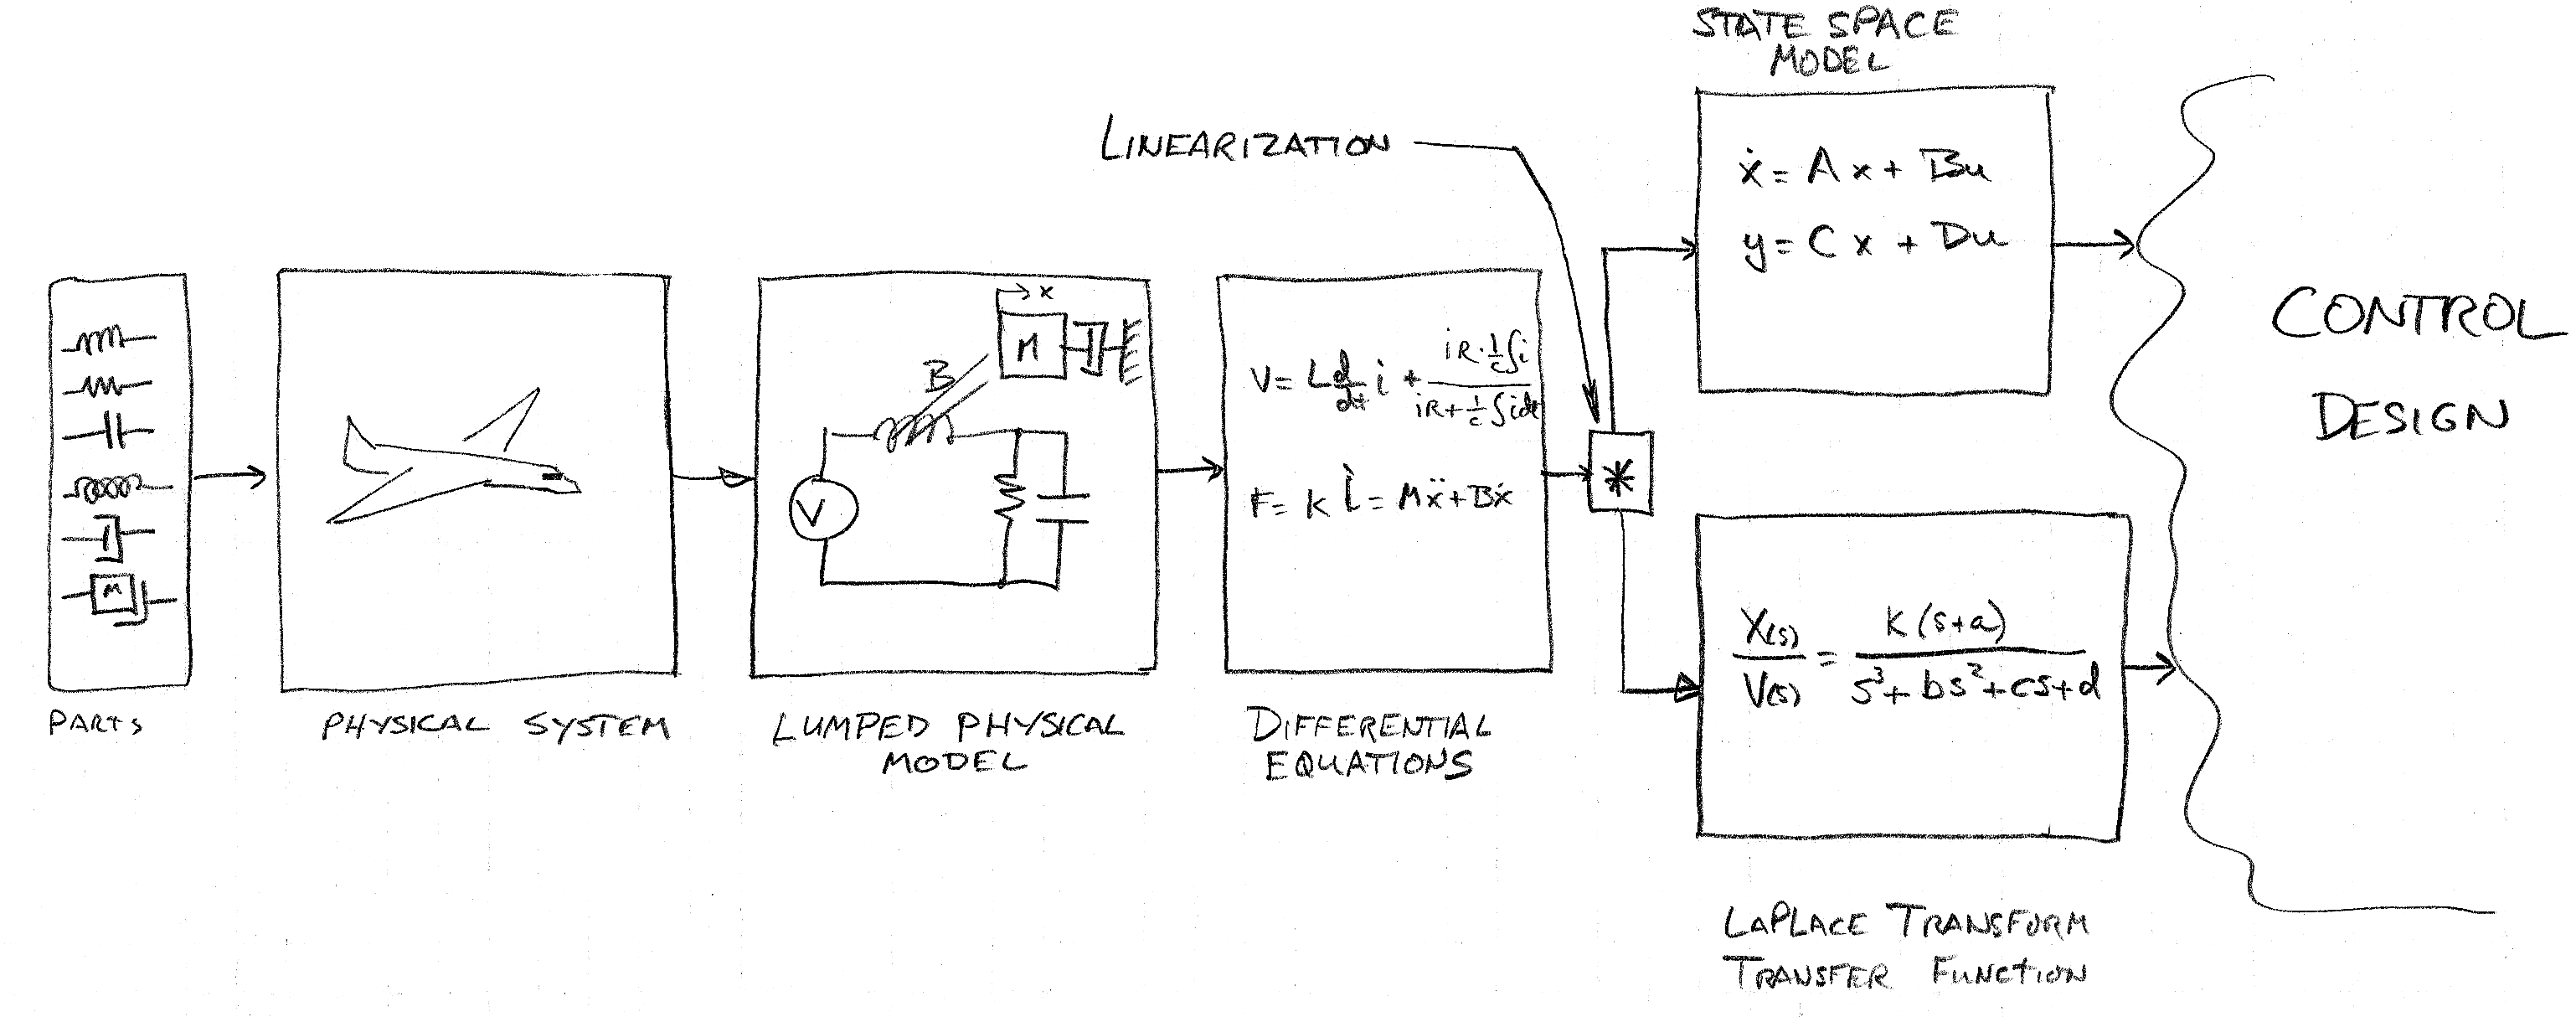
\includegraphics[width=6.45in]{figs01/01115.png}
\caption{Conceptual flow of system analysis preceding control system design.s}\label{fig_control_design_flow}
\end{figure}


%%%%** Section 2
\section{LODE}
%%%%** Section 2.1
\subsection{Basic definition}

A Linear Ordinary Differential Equation (LODE) is an equation of the form
\[
f(t) = \sum_{i=0}^{N} a_i\frac{d^i}{dt^i}x(t)
\]
The highest derivative, $N$, is referred to as the {\it order} of the LODE.  For example,
\[
f(t) = 0.273\frac{d^3}{dt^3}x(t) + 6.73\frac{d^2}{dt^2}x(t) - 0.001\frac{d}{dt}x(t) + 14.7x(t)
\]
is a third-order LODE.   Often we introduce some shorthand by omitting the time dependence ``$(t)$", and by using the dot notation for time derivatives:
\[
\dot{x} = \frac{d}{dt}x(t)  \qquad \ddot{x} = \frac{d^2}{dt^2}x(t)
\]
So that the example above would be written
\[
f(t) =0.273\frac{d^3}{dt^3}x + 6.73\ddot{x} - 0.001\dot{x} + 14.7x
\]
(you can use three dots for $\frac{d^3}{dt^3}$ if you wish.)



%%%%** Section 2.2
\subsection{Solution of First Order LODE}

A very basic  first order LODE is
\[
\dot{x} + Px = 0
\]

If we guess the solution is
\[
x(t) = e^{pt} \qquad \dot{x}(t) = pe^{pt}
\]
we can easily check it by plugging in to the original LODE:
\[
pe^{pt} +Pe^{pt} = 0 \to pe^{pt} = -Pe^{pt}
\]
giving
\[
p = -P
\]
so the solution is
\[
x(t) = e^{-Pt}
\]

Because of the partial fraction expansion (covered below), this covers a very wide variety of real world LODEs.


%%%%** Section 3
\section{Laplace Transform Review}

We will extensively use Laplace Transforms to manipulate the differential equations of control systems.  As a review, the Laplace transform is
\[
\sL \{f(t)\} = F(s) =  \int_{0}^{\infty} e^{-st}f(t)dt
\]
where $s$ is a complex variable, $s=\sigma + j \omega$.  Technically this is the ``one sided" Laplace Transform because the integral extends only to positive $t$.
The inverse of the Laplace Transform is
\[
f(t) = \sL^{-1}F(s) = \frac{1}{2\pi j} \lim_{T\to\infty} \int_{\sigma - j T}^{\sigma + jT}F(s) e^{st}ds
\]

For this course, we will not need to evaluate these integrals, because all of the LODEs we study will result in just a few terms which have been worked out long ago and are widely available in tables (Table \ref{LaplaceTransformTable}).



%%%%** Table 1
\begin{table}\centering
\renewcommand\arraystretch{2.0}% Vertical Row size, 1.0 is for standard spacing)
\begin{tabular}{|c|c|}
\hline
$ f(t)$ { for} $t \geq 0$ &  $\sL(f)$\\
\hline
$1u(t)$      & $\displaystyle \frac{1}{s}$\\\hline
$e^{at}$ & $\displaystyle \frac{1}{s-a}$\\ \hline
$t^n$    & $\displaystyle \frac{n!}{s^{n+1}}$ ($n = 0,1, \ldots$)\\ \hline
$\sin at$ & $\displaystyle \frac{a}{s^2 + a^2}$\\ \hline
$\cos at$ & $\displaystyle \frac{s}{s^2 + a^2}$\\ \hline
$\dot{f}(t)$ & $s{\cal L}(f)-f(0)$\\ \hline
$\ddot{f}(t)$ & $s^2{\cal L}(f)-sf(0)-\dot{f}(0)$
\\ \hline
\end{tabular}

(Where
$u(t) = \{ 0, t\le 0; 1, t > 0$,
$\dot{f}(t) = \frac{df(t)}{dt}$, $\ddot{f}(t) = \frac{d^2f(t)}{dt^2}$)
\caption{Table of some commonly used Laplace Transform pairs.}\label{LaplaceTransformTable}
\end{table}


When using this table we need to keep in mind a few limitations and assumptions:

\begin{itemize}
  \item We are only considering $t>0$.   One way to do this is to consider functions to be multiplied by the Unit Step function, $u(t)$

\[
  u(t) = \left \{ \begin{array}{ll}  0 & t < 0 \\ 1 & t > 0 \end{array} \right .
\]

  \item When using the differentiation relationship (last two lines of Table \ref{LaplaceTransformTable}) we must be careful about the initial conditions ($f(0), \dot{f}(0)$).    Most often, we assume that all initial conditions are zero, but it is your responsibility to verify that this assumption applies to a given problem.
\end{itemize}



%%%%** Example 1
\begin{ExampleSmall}
Find the Laplace Transform of the following time functions:  in all cases, assume the function is $0$ for $t<0$ and that initial conditions are zero

\vspace{0.2in}

\[
\sL\{55e^{-1.2t}\}
\]
Consulting the table and using the linearity property of the Laplace Transform integral:

\[
\sL\{55e^{-1.2t}\} = \frac {55} {s+1.2}
\]

\vspace{0.2in}
and

\[
\sL\{ 3.2\sin(7.6t) \} = \frac {24.32}{s^2 + 57.76}
\]
\vspace{0.2in}


\[
\sL\{ 2.6\ddot{x} - 3.52\dot{x} + 120x \} =
\]
\[
= 2.6X(s)s^2-3.52X(s)s+120X(s)
\]
\[
= X(s) \left(2.6s^2 - 3.52s + 120 \right)
\]
Note that we have assumed that $x(0) = \dot{x}(0) = \ddot{x}(0) = 0$.   Although this might seem restrictive, we often consider physical systems starting from rest (think rocket launch!) and this situation is well modeled by such zero initial conditions.
\end{ExampleSmall}


%%%%** Example 2
\begin{ExampleSmall}
Find the inverse Laplace transform of the following functions

\vspace{0.2in}

\[
\sL^{-1}\{\frac{10}{s+3.7}  \}
\]
Consulting the table and using the linearity property of the Laplace Transform integral:


\[
\sL^{-1}\{\frac{10}{s+3.7}  \}  = 10e^{-3.7t}
\]
\vspace{0.2in}
similarly

\[
\sL^{-1}\{ \frac{144s}{s^2 + 144} \}  = 144\cos(12t)
\]

\vspace{0.2in}


\[
\sL^{-1}\{ X(s)(s^3 + as^2 + bs+c) \} = \frac{d^3}{dt^3}x + a\ddot{x} + b\dot{x} + cx
\]

Here we have implicitly assumed zero initial conditions.

\end{ExampleSmall}


Let's apply the Laplace Transform to the initial LODE above.  First, we will modify the LODE to include a ``Forcing Function" on the right hand side.  A forcing function is typically a physical input to the system such as an applied voltage or force.

\[
\dot{x} + Px = f(t)
\]
Assuming zero initial conditions and taking the Laplace Transform of both sides (see the second to last line of Table \ref{LaplaceTransformTable}).
\[
sX(s) + PX(s) = F(s)
\]
\[
X(s) (s+P) = F(s)
\]
\[
\frac{X(s)}{F(s)} = \frac {1}  {(s+P)}
\]
Here we have derived a ratio called the ``Transfer Function" between position and the forcing function.  Our solution to the LODE was
\[
x(t) =  e^{pt} =  e^{-Pt}
\]
If we rewrite this using the solution, $p = -P$, then our transfer function becomes
\[
\frac{X(s)}{F(s)} = \frac {1}  {(s-p)}
\]
We call $p$ the ``pole" of this transfer function because the transfer function goes to infinity when $s=p$.



%%%%** Section 4
\section{Partial Fraction Expansion}\label{partialfractionsection}

A very useful property of polynomials is the partial fraction expansion:

\[
\frac{\prod_j (s-z_j)}{\prod_i (s-p_i)}    =  \sum_i  \frac{A_i}{(s-p_i)}
\]

In the form on the left, we have terms called $zeros$ on the top because any time $s=z_j$ the ratio is zero.  We also have terms called $poles$ in the denominator, because any time $s=p_i$, the ratio is infinite.

The partial fraction expansion is very useful for ratios of polynomials in $s$
(such as the left side above which we will encounter frequently) because such a ratio
becomes a series of terms which have an easy inverse Laplace Transform
\[
\frac{A_i}{(s-p_i)}   \leftrightarrow  A_ie^{p_it}
\]



\subsubsection{Single Poles Case}
For example,
\[
G(s) = \frac{s+5}{s^3 + 6s^2+ 358s+400}
\]
does not have an obvious inverse Laplace transform.   However if we can factor it to get

\[
G(s) = \frac  {(s+5)}   {(s+2)(s+4)(s+50)}
\]
then we can use the Partial Fraction expansion to  get it into the form
\[
G(s) = \frac{A_1}{(s+2)}+\frac{A_2}{(s+4)}+\frac{A_3}{(s+50)}
\]
then we can immediately write
\[
g(t) = A_1e^{-2t} + A_2e^{-4t} + A_3e^{-50t}
\]





It is not obvious that the partial fraction expansion is always possible but we will derive a class of cases and then perform some examples.
Let's call the exponential time constants
\[
p_1 = -2, \;p_2=-4,\; p_3 = -50
\]
and assume
\[
G(s) = \frac  {(s-z)}   {(s-p_1)(s-p_2)(s-p_3)} =  \frac{A_1}{(s-p_1)}+\frac{A_2}{(s-p_2)}+\frac{A_3}{(s-p_3)}
\]

Here we write $(s-p_1)$ because we usually are dealing with $negative$ real poles.   In other words: $(s+5) = (s - -5)$.   The real pole is $-5$ and the
term we are writing is $(s-p)$, where $p=-5$.

Now we multiply through by $(s-p_1)$:

\[
G(s) = \frac  {(s-p_1)(s-z)}   {(s-p_1)(s-p_2)(s-p_3)} =  \frac{A_1(s-p_1)}{(s-p_1)}+\frac{A_2(s-p_1)}{(s-p_2)}+\frac{A_3(s-p_1)}{(s-p_3)}
\]
Now we do two things:  1) cancel terms where possible,  2) solve for the special case $s=p_1$

\noindent
1)
\[
\frac  {(s-z)}   {(s-p_2)(s-p_3)} =  \frac{A_1}{1}+\frac{A_2(s-p_1)}{(s-p_2)}+\frac{A_3(s-p_1)}{(s-p_3)}
\]
2)
let $s=p_1$:
\[
\left . \frac  {(s-z)}   {(p_1-p_2)(p_1-p_3)} \right |_{s=p_1} =  \frac{A_1}{1}+\frac{A_2(p_1-p_1)}{(p_1-p_2)}+\frac{A_3(p_1-p_1)}{(p_1-p_3)}
\]
We can eliminate the $A_2,A_3$ terms! Giving:
\[
\frac  {(p_1-z)}   {(p_1-p_2)(p_1-p_3)} =  {A_1}
\]

Since everything on the left hand side is known,
we have just solved $A_1$.    If we multiply through by each denominator in turn, we can get all the $A_i$.




%%%%** Example 3
\begin{ExampleSmall}
Expand
\[
G(s) = \frac         {50(s+1)}                      {(s+0.1)(s+14)(s+567)}
\]
by the Partial Fraction Expansion.

\vspace{0.2in}
Solution:
\[
G(s) = \frac{A_1}{(s+0.1)} + \frac{A_2}{(s+14)} + \frac{A_3}{(s+567)}
\]

\[
A_1 = \left . \frac {(s+0.1)50(s+1)}{(s+0.1)(s+14)(s+567)} \right |_{s=-0.1} = \left . \frac {50(s+1)}  {(s+14)(s+567)}\right |_{s=-0.1}
\]
\[
= \frac {50(0.9)}{13.9\times566.9} = 0.00571
\]

\[
A_2 = \left . \frac {(s+14)50(s+1)}{(s+0.1)(s+14)(s+567)} \right |_{s=-14} = \frac {50(-13)}{-13.9 \times 553} = 0.0846
\]
\[
A_3 = \left . \frac {(s+567)50(s+1)}{(s+0.1)(s+14)(s+567)} \right |_{s=-567} = \frac {50(-566)}{-566.9 \times -553} = -0.090
\]
\vspace{0.15in}
\[
G(s) = \frac{0.00571}{(s+0.1)} + \frac{0.0846}{(s+14)} + \frac{-0.090}{(s+567)}
\]
\end{ExampleSmall}

%%%%** Example 4
\begin{ExampleSmall}
Use the Partial Fraction Expansion to find the inverse Laplace Transform of
\[
G(s) =  \frac          {27}             {(s+50)(s+3000)}
\]


\[
A_1 = \left . \frac {(s+3000)27}{(s+50)(s+3000)} \right |_{s=-3000} = \frac {27}{-2950} = -0.00915
\]
\[
A_2 = \left . \frac {(s+50)27}{(s+50)(s+3000)} \right |_{s=-50} = \frac {27}{2950} = 0.00915
\]

\[
g(t) = 0.00915(e^{-50t}-e^{-3000t})
\]

\end{ExampleSmall}



Sometimes the poles are complex conjugates\footnote{Recall that complex poles always come in complex conjugate pairs if our
system parameters such as $M,B,K,J,$ etc are real numbers.}, there are further simplifications possible after the Partial Fraction Expansion.




%%%%** Example 5
\begin{Example}

Find
\[
\sL^{-1}\{G(s) = \frac{(s+5)}{(s+6)(s+2+j)(s+2-j)}\}
\]

\vspace{0.25in}

Using the techniques above we can get:

\[
A_1 = -1/17 = -0.059 \qquad A_2 = 0.029+0.38j \qquad A_3 = 0.029-0.38j
\]
(note that it is not necessary to compute $A_3$ because it will always be the case for complex conjugate poles that $A_{n+1} = A_n^*$.)
\[
G(s)  = \frac {-0.059} {(s+6)}  + \frac {0.029+0.38j} {(s+2+j)}  + \frac {0.029-0.38j} {(s+2-j)}
\]

Applying the inverse transform to each term:

\[
g(t) = -0.059e^{-6t} + (0.029+0.38j)e^{(-2-j)t}+ (0.029-0.38j)e^{(-2+j)t}
\]

First, let's approximate
\[
0.029\pm 0.38j \approx 0.38e^{\pm j \pi/2}
\]
by 1) ignoring the small real part and
2) converting to Magnitude-Angle form (see Appendix \ref{ComplexNumberReview}).

\[
g(t) = -0.059e^{-6t} + 0.38e^{j\pi/2}e^{(-2-j)t} + 0.38e^{-j\pi/2}e^{(-2+j)t}
\]
\[
g(t) = -0.059e^{-6t} + 0.38e^{-2t} \left ( e^{j(-t+\pi/2)}+e^{-j(-t+\pi/2)} \right )
\]
Where we used:
\[
e^{j\pi/2}\cdot e^{(-2-j)t} \to e^{(j\pi/2-2t-jt)} \to e^{(-2t+j(\pi/2-t))} \to  e^{(-2t)}\cdot e^{j(\pi/2-t))}
\]
Now we use Euler's famous equality
\[
e^{j\theta} = \cos(\theta) + j \sin(\theta)
\]
as follows:
\[
g(t) = -0.059e^{-6t} + 0.38e^{-2t} \left (
    \cos(-t+\pi/2) + j\sin(-t+\pi/2)+
    \cos(-t+\pi/2) - j\sin(-t+\pi/2)
    \right )
\]
Since $\cos(\theta) = -\cos(\theta)$, and $\cos(\theta-/pi/2) = \sin(\theta)$

\[
g(t) = -0.059e^{-6t} + 0.38e^{-2t} \left (
    2\cos(t-\pi/2)
    \right )
\]
\[
g(t) = -0.059e^{-6t} + 0.76e^{-2t} \left (
    \cos(t-\pi/2)
    \right )
\]
\[
g(t) = -0.059e^{-6t} + 0.76e^{-2t} \left (  \sin(t)  \right )
\]

\end{Example}



%%%%** Example 5
\begin{ExampleCont}
By throwing a few values of $t$ into the calculator,
we can generate a sketch of the second term as shown below:
$ 0.76e^{-2t} \left (  \sin(t)  \right )$

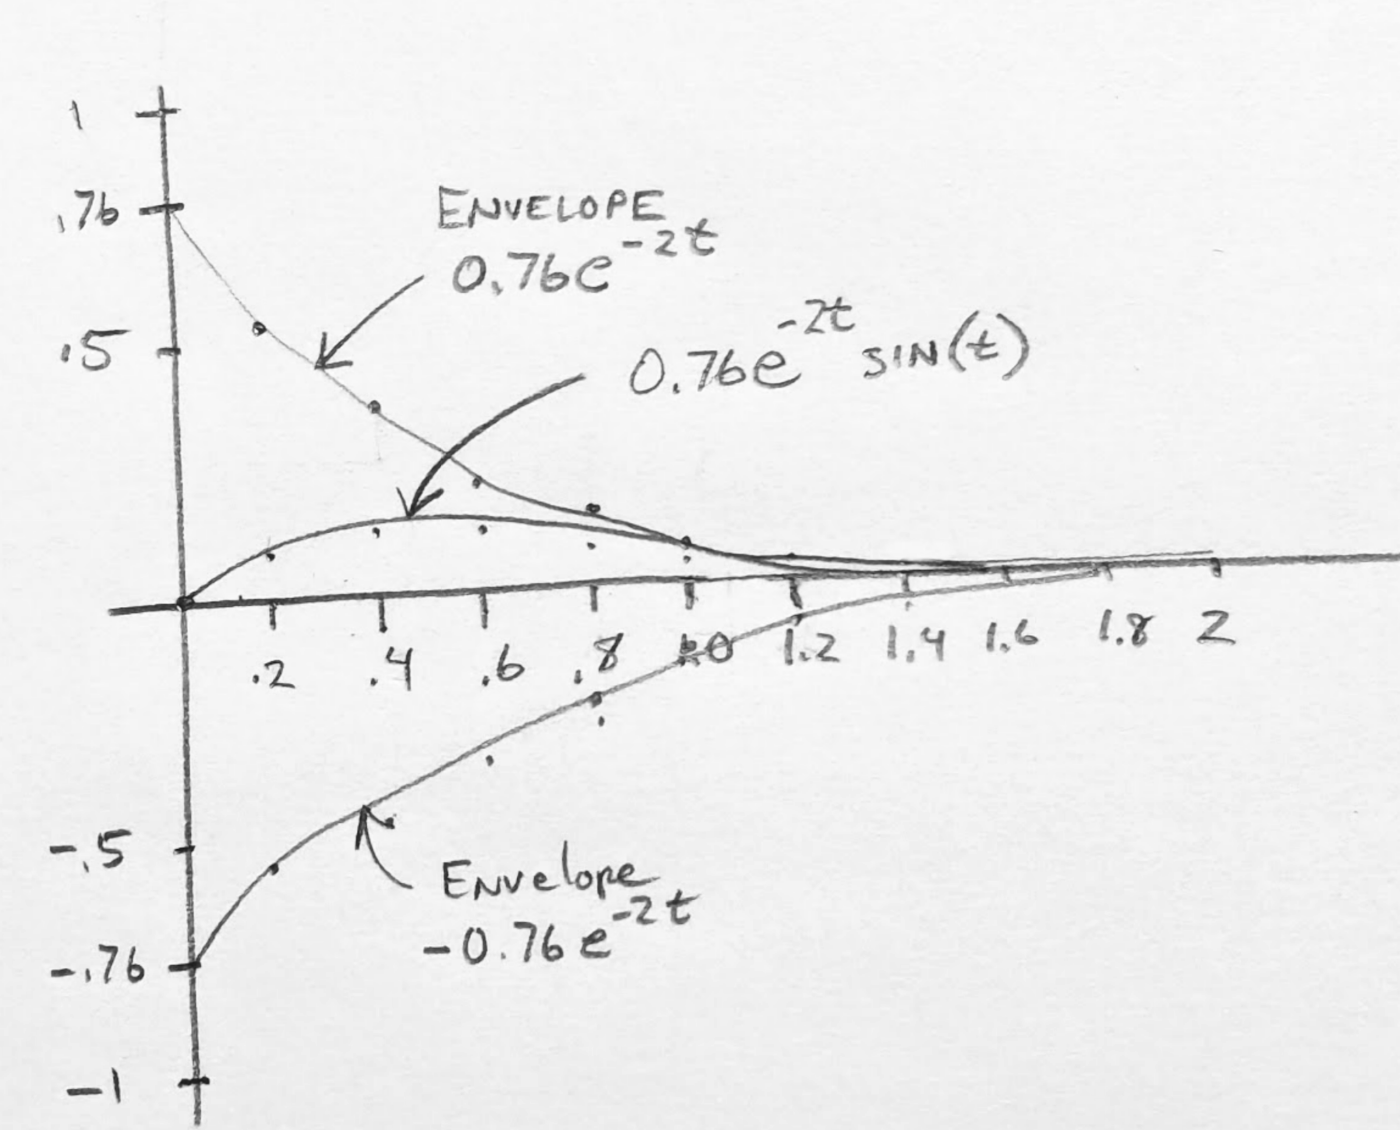
\includegraphics[width=82mm]{figs01/J55Q14.png}

For a more accurate plot, let's use the computer on the final result(including both terms):
\[
g(t) = -0.059e^{-6t} + 0.76e^{-2t} \left (  \sin(t)  \right )
\]

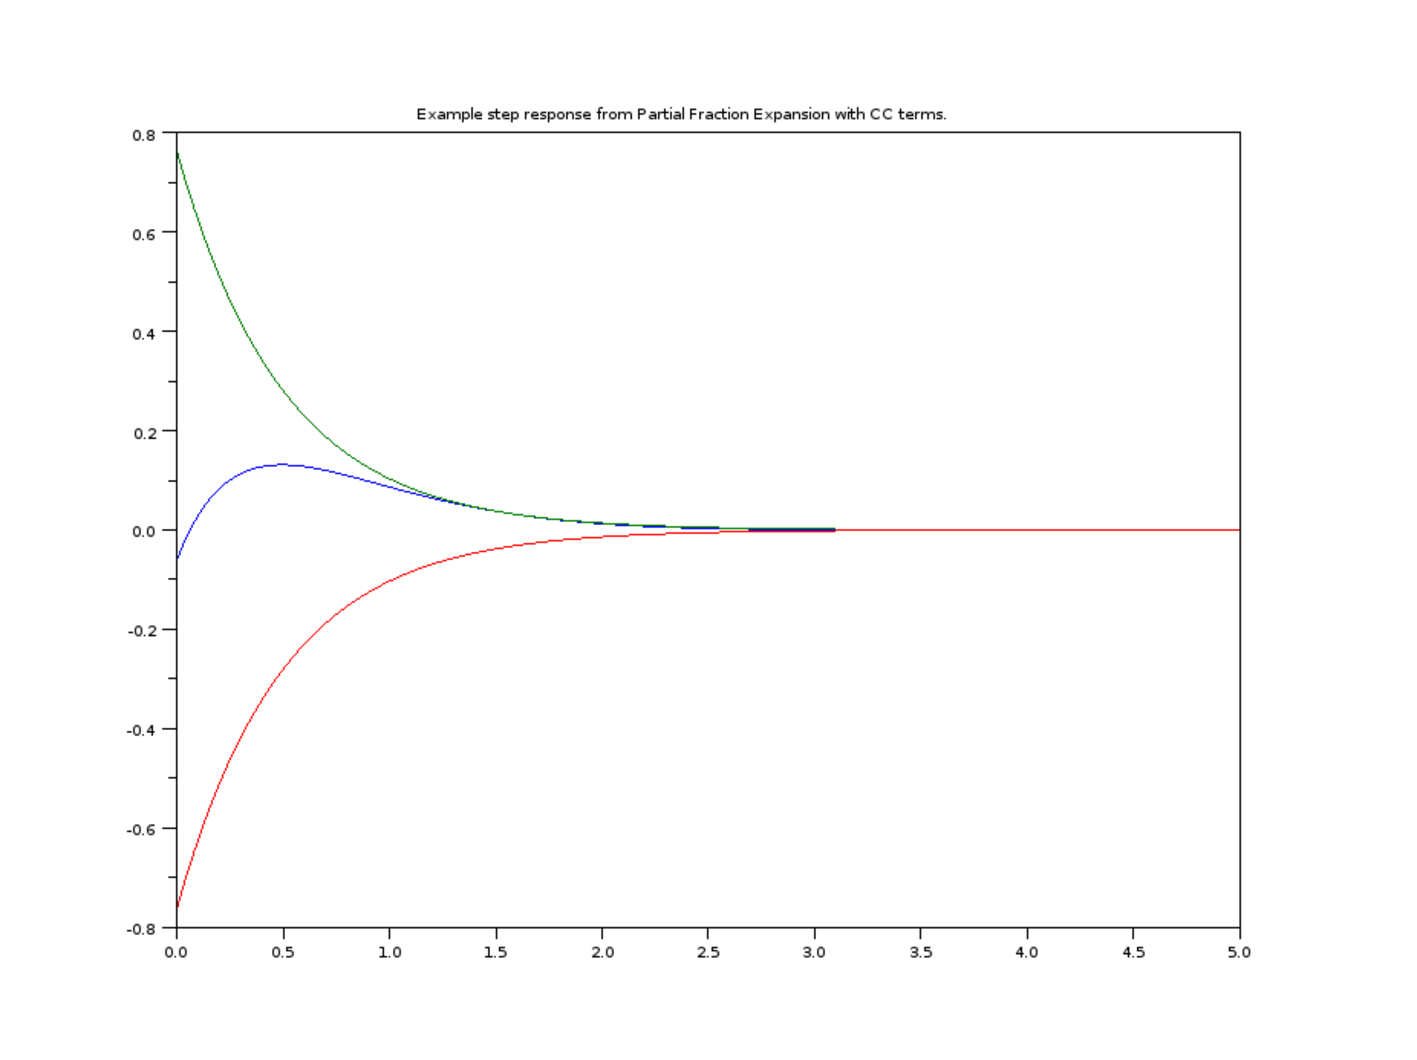
\includegraphics[width=120mm]{figs01/pf_compConja.png}


\end{ExampleCont}

\subsubsection{Repeated Poles}

Another situation comes when a pole is repeated (i.e. $\frac{1}{(s+2)^2}$).  In this case the trick we use for the partial fraction expansion no longer works!   But instead we can still solve for $A_i$ by differentiating the partial fraction expansion.

%%%%** Example 6
\begin{ExampleSmall}
Apply the Partial Fraction Expansion to
\[
G(s) = \frac {(s+5)}  {s^2(s+3)}
\]
(note that there is a repeated root  in the demoninator (repeated pole at $s=0$)).

We start by setting up the problem with two terms for the repeated pole:

\[
G(s) = \frac {A_1}{s^2} +  \frac {A_2}{s} +  \frac {A_3}{(s+3)}
\]
$A_1$:

\begin{equation}\label{eqn1Ex1p6}
\left . \frac{s^2(s+5)} {s^2(s+3)}\right |_{s=0}  = \frac {s^2A_1}  {s^2}   + \frac{s^2A_2} {s} + \frac {s^2A_3} {(s+3)}
\end{equation}
giving
\[
A_1 = 5/3
\]

$A_3$ is also straightforward, giving $A_3 = 2/9$. But working through $A_2$ we find:

\[
\left . \frac{s(s+5)} {s^2(s+3)}\right |_{s=0}  = \frac {sA_1}  {s^2}   + {A_2}  + \frac {sA_3} {(s+3)}
\]

We now have the problem that we cannot cancel the $s^2$ in the denominator of the $A_2$ term (which we need to do!).   Instead differentiate the $A_1$ expression (Eqn. \ref{eqn1Ex1p6} with respect to $s$:
\[
\frac{d}{ds}\frac{(s+5)}{(s+3)} = 0 + A_2 + \frac{d}{ds} \frac{s^2}{(s+3)}A_3
\]
Using an advanced differentiation rule (below) gives:
\[
\frac{-2}{(s+3)^2} = A_2 + \frac{s(s+6)}{(s+3)^2}A_3
\]
evaluating at $s=0$,
\[
A_2 = -2/9
\]
The tricks we used used:
\[
\frac{d}{dx}\frac{(x+a)}{(x+b)} = \frac{1}{(x+b)} - \frac{(x+a)}{(x+b)^2}
\]
and
\[
\frac{d}{dx} \frac{x^2}{(x+a)} = \frac{2x}{(x+a)} - \frac{x^2}{(x+a)^2}
\]

This gets even more unwieldy when the repeated pole is non-zero, but fortunately we rarely need this technique or can fall back on numerical
or AI-based symbolic methods.
\end{ExampleSmall}




%%%%** Section 5
\section{Linearization}

\subsection{Overview}
Laplace Transforms can only be used on linear equations.  In most of this course we focus on linear differential equations but often real world applications involve non-linear functions.   All is not lost if we can usefully {\it approximate} our non-linear function with a linear one.  Our approach to linearization is to model the original function with a straight line.


Consider a nonlinear function, $f(x)$.  The linearized version of $f(x)$, $\hat{f}(x)$,  can be constructed about a specific operating point, $x_0$.

\[
\hat{f}(x) = f(x_0) + \frac{d}{dx}f(x_0) (x-x_0)
\]

$\hat{f}(x)$ is a linear function of $x$ which is most accurate in the neighborhood of $x_0$.   It is also the  first two terms of a Taylor series expansion of $f(x)$.   It is very helpful to visualize this process graphically by plotting the linearized function on top of the original function (Figure \ref{locallinearizationSketch}).

\begin{figure}\label{locallinearizationSketch}
  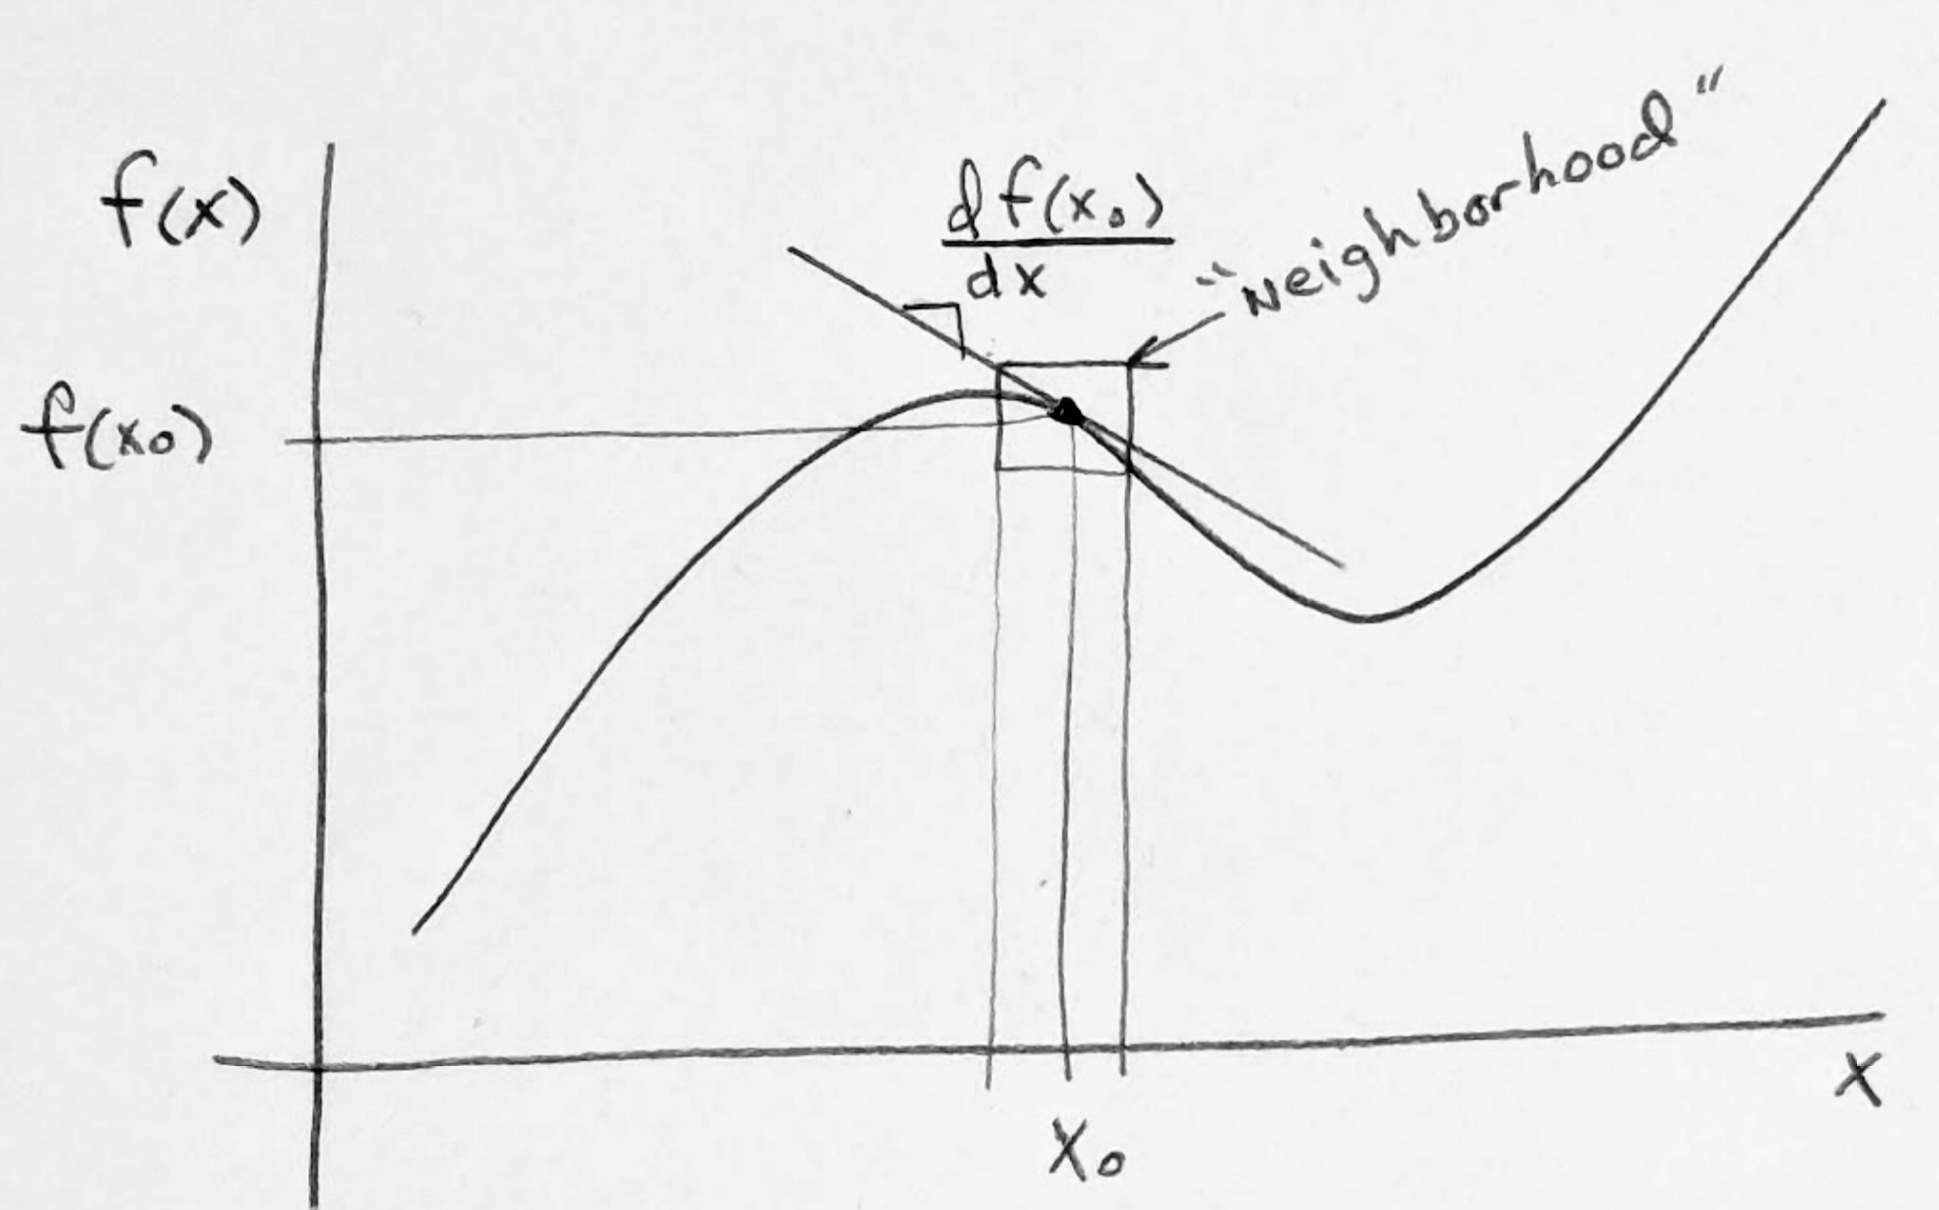
\includegraphics[width=105mm]{figs01/Q75B05.png}
  \caption{Illustration of a linearized version of a non-linear function at an operating point.}
\end{figure}
\clearpage



\subsection{Linearization Examples}
%%%%** Example 7
\begin{ExampleSmall}\label{twolinexamples}

Consider the nonlinear function
\[
f_1(x) = 0.4x^2 -0.1x^3 + 3\sin(x)
\]
and linearize twice, once about $x=-6$, and again about $x=1$ (we are using radians for $\sin(x)$).

\vspace{0.2in}

First evaluate $f_1(x)$ for the two linearization points:
\[
f_1(-6) = 36.84 \qquad  f_1(1) = 2.824
\]
Then let's get the derivative:

\[
\dot{f}(x) = 0.8x -0.3x^2 +3\cos(x)
\]
and evaluate it at the two points:

\[
\dot{f}(-6) = -12.72 \qquad \dot{f}(1) = 2.121
\]

Now we get:

\[
\hat{f}_{1a} = 36.84-12.72(x+6) = -39.48-12.72x \qquad \hat{f}_{1b} = 2.824+2.121(x-1) = 0.703+2.121x
\]

Plotting using the computer:
\begin{center}
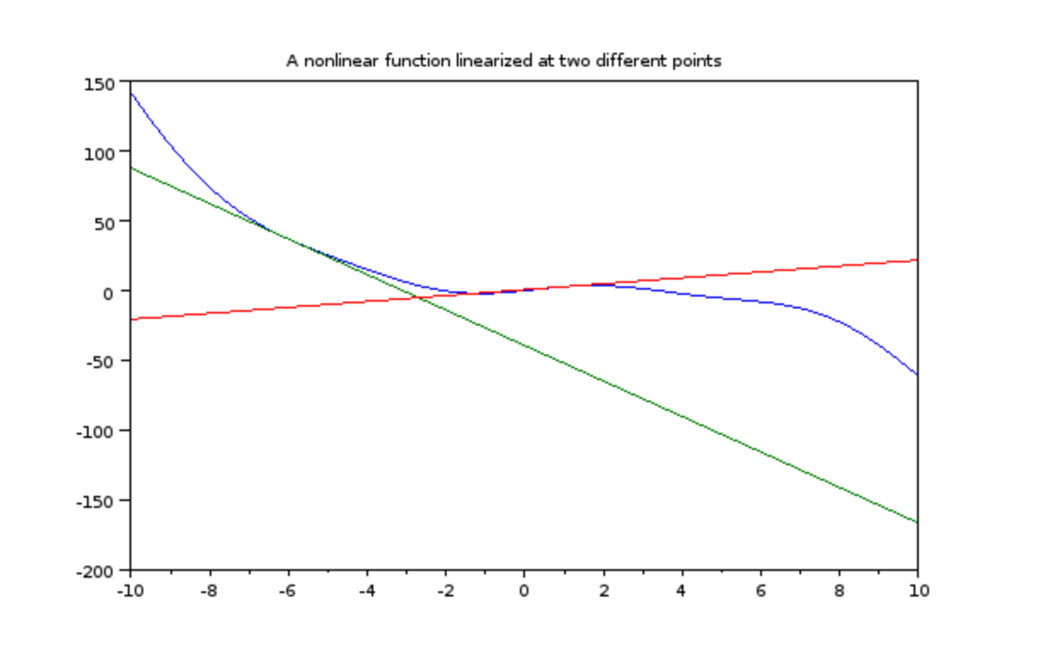
\includegraphics[width=3.5in]{figs01/linearizeattwopointsa.png}
\end{center}

The blue line is $f(x)$, the green line is $\hat{f}_{1a}(x)$ and the red line is $\hat{f}_{1b}(x)$.  The linear approxmations are reasonably accurate in the neighborhood of their operating points ($x = -6, +1$), but become very bad as we move away.  The size of the ``neighborhood" for which a degree of accuracy can be obtained depends on the function and the selected operating point.

\end{ExampleSmall}


Some combinations of functions and operating points are especially easy to linearize.

%%%%** Example 8
\begin{ExampleSmall}
Linearize
\[
f_2(x) = 0.723x^3 -4.37x^2 +67x
\]
about the point $x=0$
\vspace{0.2in}

\[
f_2(0) = 0
\]
\[
\frac{d}{dx}{f}_2(x) = 2.169x^2 - 8.74x + 67
\]
\[
\frac{d}{dx}{f}_2(0) = 67
\]
\[
\hat{f}_2(x) =  67x
\]
Note that we are simply taking the linear term of $f_2(x)$, $67x$.
However we only could get away with this because 1) we linearized about $x=0$ and 2) the function was a polynomial.
\end{ExampleSmall}

%%%%** Example 9
\begin{ExampleSmall}
Linearize $f_2(x)$ from the previous example about $x=5.7$
\vspace{0.2in}

\[
f_2(5.7) = 373.81
\]
\[
\frac{d}{dx}{f}_2(5.7) = 87.6521
\]
\[
\hat{f}_{2a}(x) = 373.81 + 87.6521(x-5.7)
\]
\[
\hat{f}_{2a}(x) = -125.81 + 87.6521x
\]
This is quite different from $\hat{f}_2(x)$.  So only if we carefully use the two rules of the previous example, we
can linearize by simply deleting all terms except the linear term.

\end{ExampleSmall}


When the equation to be linearized is a differential equation,
% we introduce a slightly strange notion: taking the derivative with respect to a derivative:
just

\begin{enumerate}
  \item isolate the non-linear part
  \item treat it like a simple function
  \item linearize the function
  \item plug the function back into the differential equation
\end{enumerate}

%%%%** Example 10
\newpage\begin{ExampleSmall}
Linearize the differential equation
\[
f_3(t) =   \ddot{x} - 0.42\dot{x} + 0.01(\dot{x})^3 + \sin(5\dot{x}) + 16x
\]
about $\dot{x} = 0$  (We have omitted $(t)$ from $\{x(t), \dot{x}(t),\ddot{x}(t)\}$ to simplify notation.)
$\dot{x}$ is often the velocity of a physical part.
Does a system do anything interesting if $\dot{x} = 0$?  It can.  Remember the linearization works
in the {\it neighborhood} of the operating point -- so we could say this linearization is valid for slow speeds
(velocities near zero).  That might be what we care about in our application.


\vspace{0.2in}
The nonlinear part of this differential equation can be taken out as a simple function, $Fn()$:
\[
Fn(y) = 0.01y^3+\sin(5y)
\]
where we are using the variable $y$ just to avoid confusion with $x,\dot{x}$.   Now we linearize $Fn(y)$ about $y=0$:
\[
\frac{d} {dy}Fn(y)  = 0.03y^2+5\cos(5y)
\]
\[
\hat{F}n(y) = Fn(0) + \left . \frac{d} {dy}Fn(y) \right|_{y=0} (y-0) = 0 + 5\cos(0)y = 5y
\]\[
\hat{F}n(y) = 5y
\]
Plugging the linearized function back into the differential equation:
\[
f_3(t) =   \ddot{x} - 0.42\dot{x} + \hat{F}n(\dot{x}) + 16x
\]
\[
f_3(t) =   \ddot{x} - 0.42\dot{x} + 5\dot{x} + 16x = \ddot{x} + 4.58\dot{x} + 16x
\]
This LODE is a linearized version of our system which is valid in the neighborhood of $\dot{x}=0$ (i.e. for low velocities).
\end{ExampleSmall}


\subsection{Range of Approximation}
We have seen that linearization ``works" ``in the neighborhood" of the linearization point.   Here we will dive deeper into what
we mean by ``works" and ``neighborhood".

First we must define our requirement for accuracy (i.e. how much error we can have while the approximation still ``works").
Often this is dictated by some external requirement.  For example,
\begin{quotation}
The linearized model shall have less than 10\% error.
\end{quotation}
By this we mean that if we define a linear function $\hat{f}(x)$ which is a linear approximation of a non-linear function,
$f(x)$, about the point $x = x_0$ then
\[
\frac   {|f(x)-\hat{f}(x)| } {f(x)} < 0.10
\]
% We choose $f(x_0)$ as the denominator since it defines the scale for our local function.

Second, we must define ``neighborhood".    By this we mean the range of $x$ values for which the approximation is good enough (i.e. ``works").   Suppose we have
\[
x_{min} < x_0 < x_{max}
\]
such that

\[
\frac   {|f(x_{min})-\hat{f}(x_{min})| } {f(x_{min})} = 0.10
\]
and

\[
\frac   {|f(x_{max})-\hat{f}(x_{max})| } {f(x_{max})} = 0.10
\]

Assuming that $f(x)$ changes slowly, we can call the ``neighborhood"
\[
x_{min} < x < x_{max}
\]
the region where the approximation is sufficient.



\begin{Example}
Consider the system of Example \thechapter.\ref{twolinexamples}.  The equations were:

\[
f_1(x) = 0.4x^2 -0.1x^3 + 3\sin(x)
\]
 linearized twice, once about $x=-6$ radians, and again about $x=1$ radian.


\[
\hat{f}_{1a} =  -39.48-12.72x \qquad \hat{f}_{1b} =  0.703+2.121x
\]

If the accuracy requirement is 5\%, which linearization $a$ or $b$ has a bigger ``neighborhood"?


Our approach will be to compute numerically values of $f(x)$ and $\hat{f}(x)$ and look for the error dropping below 5\%
We'll define our error percentage as:
\[
E_j = \left| \frac {f(x) - f_j(x)} {f(x)}  \right |
\]

Let's make a spreadsheet for them both.  We'll generate columns as follows:

\begin{tabular}{|c|c|c|c|c|c|}\hline
A & B & C & D & E & F \\ \hline
$x$  & $f_1(x)$ & $f_{1a}(x) $  &  $E_a$ & $f_{1b}(x) $ &  $E_b$ \\
\hline
\end{tabular}


\begin{tabular}{cp{0.4\textwidth}}
\begin{minipage}{0.45\textwidth}
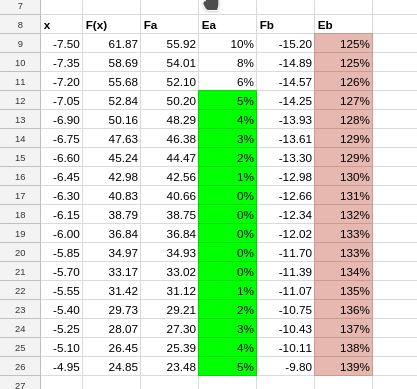
\includegraphics[width=\textwidth]{figs01/lin_sheet_01.png}
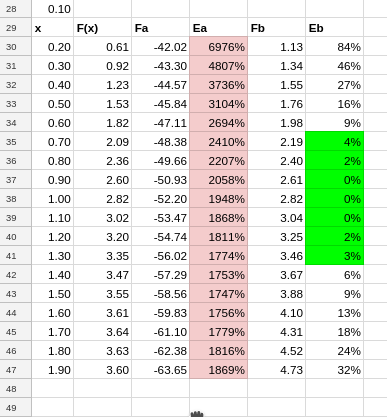
\includegraphics[width=\textwidth]{figs01/lin_sheet_02.png}
\end{minipage}

&

\begin{minipage}{0.45\textwidth}
\begin{center}
{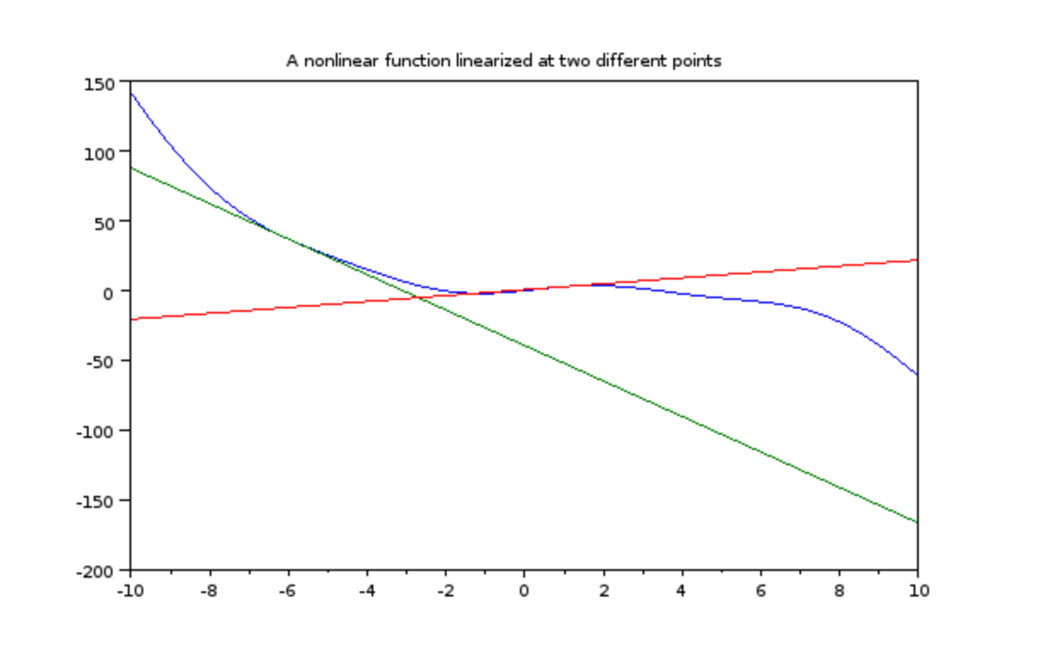
\includegraphics[width=\textwidth]{figs01/linearizeattwopointsa.png}}
\end{center}

There are two sets of rows, one centered around each linearization point ($x=-6$, and $x=1$).
Colors indicate good and bad accuracy.  The green box shows the $\pm5\%$ zone.  Note how
$f_{1a}$ is accurate near $x=-6$ and $f_{1b}$ is accurate near $x=1$.

Answering our specific question, the range for $f_{1a}$ is
\[
-7.04 < x < -4.95 =  2.09
\]
and for $f_{1b}$
\[
0.70 < x < 1.30 = 0.6
\]
So $f_{1a}$ has a bigger ``neighborhood".    However we are usually forced to pick the linearization point from
an application requirement so in the real world we can't just choose our linearization point according to how well linearization fits. For example, if a model of room climate control requires linearization, we MUST linearize about $T=70^\circ F$ or something close to that because we have to operate in the range of human comfort.
\end{minipage}

\vspace{0.35in}



\end{tabular}

\end{Example}





























% \section{Summary of Notation}

   % Introduction: LODE & LT  review
% %
%
%

\chapter{Translational Dynamical Systems}

\section{Problem Statement and Learning Objectives}
Be able to
\begin{itemize}
  \item Name system elements and write and graph constitutive relations for the basic elements
  of a translational mechanical system.
  \item Write the Equations of Motion for a translational system with any number of masses, springs, and dampers.
  \item Convert from Equations of Motion to a Transfer Function
\end{itemize}

\section{System Elements}

Translation refers to motion in a straight line.   We will first consider systems which only contains elements moving along a single direction.  Sometimes it is useful to think of this direction as a set of different but parallel axes, but this distinction does not change the physics. We only consider such systems which operate in an inertial frame such as the surface of the earth (to a good approximation at least) or inside
a vehicle moving at constant speed and direction.

% We will view the system as consisting of two types of elements:  ``active" and ``passive".  The passive elements can store or dissipate energy but cannot generate any.   The active

We will analyze systems consisting of
\begin{itemize}
  \item {\bf Mass}        The property of matter which resists acceleration, is acted on by gravity, and which stores kinetic energy.
  \item {\bf Stiffness}   The property of matter which resists displacement, and which stores potential energy.
  \item {\bf Damping}     The property of matter or interactions of matter which converts motion to heat.
\end{itemize}

Some properties of the various elements are summarized in Table \ref{TransElementsTable}.

% \setlength\extrarowheight{0.75in}
\begin{table}
\begin{tabular}{|l|l|l|l|p{2.0in}|} \hline
 Name             &  Physical Realization     &   Symbol    &  Equation              & Units and Notes   \\ \hline
  Inertia         &  Point Mass               &   $M$ \raisebox{-\totalheight}{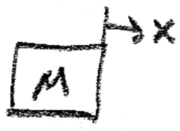
\includegraphics[width=0.6in]{figs02/00728aa.png}}     &  $f(t) = M\ddot{x}$    & $kg$, $\ddot{x}$ is with respect to the inertial frame.  \\ \hline
  Stiffness       &  Massless Spring          &   $B$ \raisebox{-\totalheight}{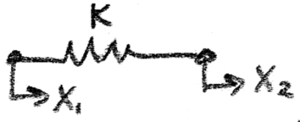
\includegraphics[width=1.0in]{figs02/00728ba.png}}    &  $f(t) = K{x}$         & $N\;m^{-1}$, $f$ is same on both sides.  Assume zero rest length \\ \hline
  Damping         &  Shock Absorber           &   $K$ \raisebox{-\totalheight}{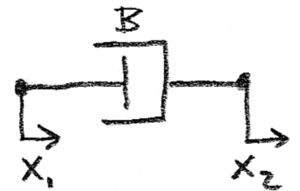
\includegraphics[width=1.0in]{figs02/00728ca.png}}   &  $f(t) = B\dot{x}$     & $N\;sec^{-1}\;m^{-1}$, This is a linear model for friction.     \\ \hline
\end{tabular}\caption{}\label{TransElementsTable}
\end{table}


\subsection{Displacements and Derivatives}

We shall analyze the state and the motion of translational systems in terms of

Position, $x(t)$, Velocity, $\dot{x}(t)$, and Acceleration, $\ddot{x}(t)$.
Where each dot represents a time derivative:
\[
\dot{x} = \frac{d}{dt}x(t) \qquad \ddot{x} = \frac{d^2}{dt^2}x(t)
\]

Often we will omit the time dependence, i.e. $\dot{x} = \dot{x}(t)$.



\subsection{Forces}

Each system element generates forces according to well known physical laws:

\begin{itemize}
  \item Mass:  $F=m\ddot{x}$.
  \item Stiffness:  $F= K(x_2-x_1)$
  \item Damping:    $F= B(\dot{x}_2- \dot{x}_1)$
\end{itemize}

In the case of stiffness and damping, the force is generated by the {\it difference} of two displacements or velocities.   In the case of Mass undergoing translational motion in an inertial frame, the force is generated only by accelerations with respect to the inertial frame.   An inertial frame is one which is not accelerating.


\subsection{Mechanical Network Schematic Diagram}

We must usually simplify the mechanical system into a purely translational one to apply the analyis of this chapter.   To do so, we identify the mass for each moving part and draw it as a box labeled $M_i$ (Figure \ref{masses}).   What each box actually represents is a point mass.  Each point mass has a displacement, $x_i$ which indicates its location along the axis of linear motion.



\begin{figure}\centering
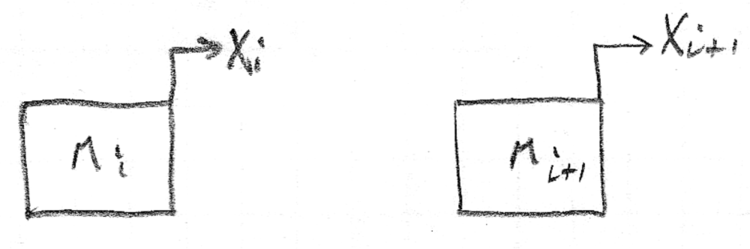
\includegraphics[width=2.5in]{figs02/00720a.png}
\caption{Each mass has an associated displacement.}\label{masses}
\end{figure}


Springs and dampers are then connected between the moving parts.   Alternatively, one end of a spring or damper may be connected to ground (a point at which $x = \dot{x} = \ddot{x} = 0$).

\begin{Example}\label{ExampleCarSuspension}

Convert the tire, wheel, and suspension elements of a typical car to a linear mass-spring-damper model.


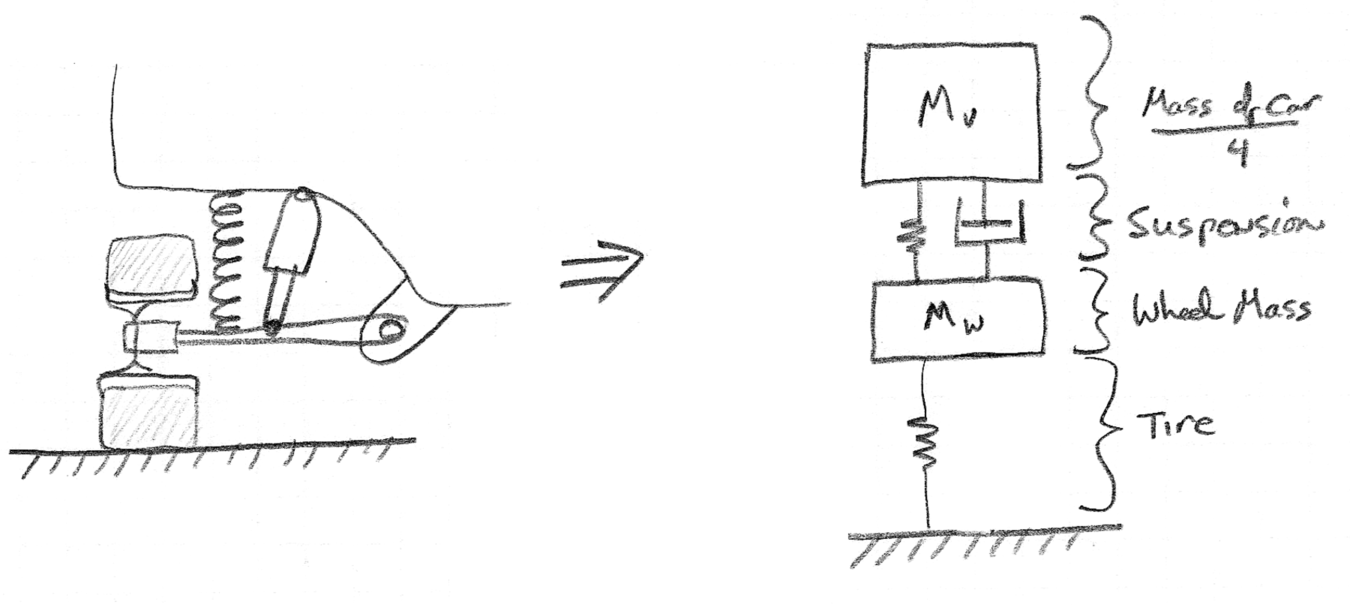
\includegraphics[width=4.5in]{figs02/00719a.png}


In this conversion we have used lots of knowledge about cars including the following facts:


 \begin{itemize}
   \item Tires are elastic and filled with a low mass material (air) and thus could plausibly be approximated by a spring.
   \item The weight of the wheel and tire can be combined into a mass.
   \item The suspension spring goes between the suspension beam and the car's body.
   \item Cars have four wheels so the mass of the body should be approximated by 1/4 of the car's total mass.
   \item The shock absorber is a damper which connects between the suspension arm and the car body (in parallel with the spring)
   \item The suspension arm is long enough compared to the tire's motion such that we can approximate the tire's motion as a straight vertical line.
 \end{itemize}


None of this knowlege is required to excel at control systems design with one exception, {\it The control system designer must have enough knowlege of the application system or access to enough model validation data to make sure that the simplified model is good enough for all application requirements. } To the extent that these ``facts" are true, our model is accurate, and to the extent that this model is an oversimplification, our model will not work.


\begin{quotation}``It can scarcely be denied that the supreme goal of all theory is to make the irreducible basic elements as simple and as few as possible without having to surrender the adequate representation of a single datum of experience." \\
{\it Albert Einstein}
\end{quotation}

\end{Example}


\section{Constitutive Relations}
Constitutive Relations are basic equations that define our system components by relating one variable to another.  For example,
a resistor relates voltage to current by Ohm's Law, $V=IR$ or a damper relates force to velocity, $F=B\dot{x}$.   Using the
analogy between force and voltage, and velocity to current, we can classify variables as ``through" or ``across" types.  Specifically

\vspace{0.25in}
\begin{tabular}{l|c|l}
           & through & across\\ \hline
Electric   & current  & voltage \\
Translation & velocity & force \\
Rotation   & angular vel.  & torque
\end{tabular}

Constitutive Relations are conventionally famous linear  functions such as
 \[
 V=IR, \; F= B\dot{x},\; F=M\ddot{x}, \quad \mathrm{etc.}
 \]
as such they are always the same graph!

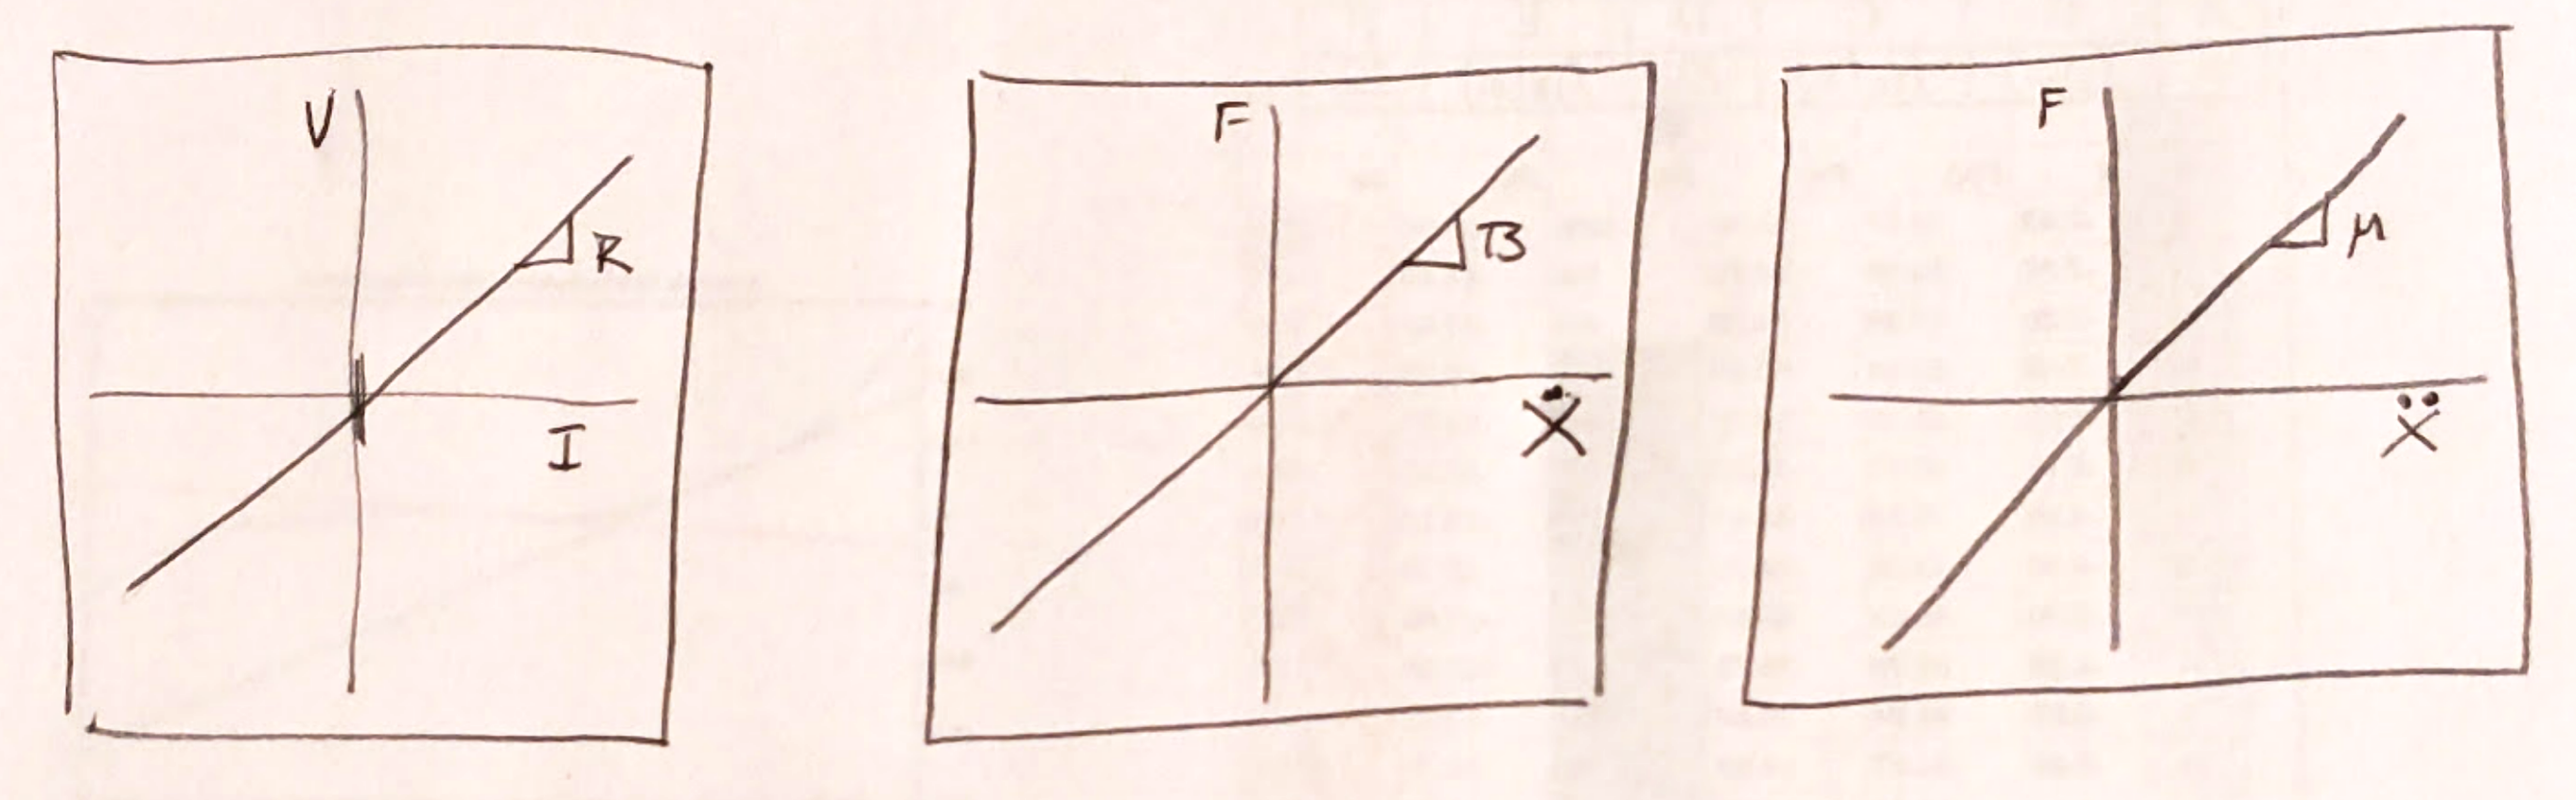
\includegraphics[width=150mm]{figs02/Q68B24.png}



\section{Equations of Motion}

Let's assume a system componsed of multiple masses connected by springs and dampers among each other.   A force $F_i$ acts on each mass, $M_i$.   D'Alembert's Principle equates the famous inertial force $f=m\ddot{x}$ to all the other forces acting on a body.   In a form that we will use:

\bq\label{D'Alembert}
M_i \ddot{x} + \sum_j B_j(\dot{x}_i - \dot{x}_j) + \sum_k K_k(x_i - x_k) = F_i
\eq

where there are several damping components connected between the mass $M_i$ and other masses indicated by $j$, and there are several
spring components connected to some other masses indicated by $k$.  We write this equation for each mass in the system.

Equation \ref{D'Alembert} is refered to as an Equation of Motion (EOM).

$F$ indicates external forces imposed on the mass from sources other than springs and dampers in the system such as an actuator.  If the translational system is vertical, the force of gravity would be one such force, $F=Mg$.

The signs in equations of motion can be tricky.   There is really no ``correct" sign for each term, because the equation is valid if you multiply both sides by $-1$.   However if we stick with the following rules, we can write equations of motion in a consistent way so that we can easily keep signs straight:

\begin{itemize}

  \item The positive term in each subtraction associated with $B$ and $K$ must be the displacement of the mass for which the current EOM is being written.
  \item Keep all position sign conventions consistent.  For example, all displacments positive ``to the right" or positive ``facing up".
  \item Keep the sign convention of the external applied force the same as for the displacements and keep it alone on the right-hand-side.

\end{itemize}






\begin{ExampleSmall}

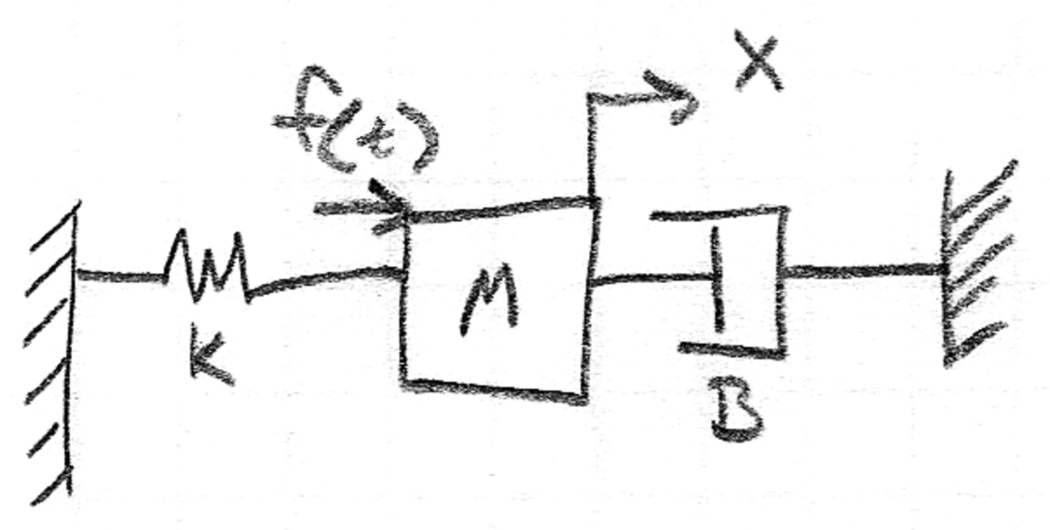
\includegraphics[width=3.0in]{figs02/00721a.png}

writing the EOM for this one mass:

\[
M\ddot{x} + B(\dot{x} - 0) + K(x-0) = f(t)
\]

The spring and damper are each connected to ground.  Ground is a point defined by $x=0$, and $\dot{x}=0$.   Here we have shown $-0$ in the EOM damping and stiffness terms for completeness.
Normally when we have springs and dampers grounded we can skip the subtraction step and the EOM is simply:

\[
M\ddot{x} + B\dot{x} + Kx = f(t)
\]

\end{ExampleSmall}





\begin{ExampleSmall}\label{example2dampers}
Here we have still a single mass, but multiple dampers are connected.   Note that it makes no difference if the ``ground" symbol is located to the left or right of the mass, it still represents $x=0, \dot{x}=0$.



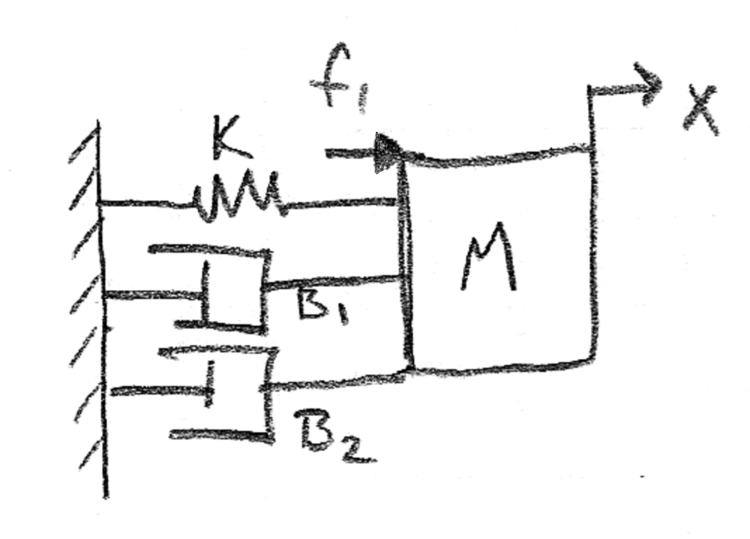
\includegraphics[width=2.5in]{figs02/00722a.png}


EOM:
\[
M\ddot{x} + B_1(\dot{x}-0)+B_2(\dot{x}-0)+K(x-0) = f(t)
\]
Simplifying

\[
M\ddot{x} + (B_1+B_2)\dot{x}+Kx = f(t)
\]
\end{ExampleSmall}


\subsection{Parallel and Series Combinations}
We were able to simplify the EOM in Example \thechapter.\ref{example2dampers} in a way which added the two dampers together.   If you think about a simple modification to Example \thechapter.\ref{example2dampers}, you can see that the same could be done with springs as well.
The general principle is that springs and dampers combine (like capacitors in electric circuits) (Figure \ref{seriessprings}) as follows:

Springs and dampers in {\it parallel} can be combined by addition.

Springs and dampers in {\it series}   can be combined like parallel resistors:

\begin{figure}[h]\centering
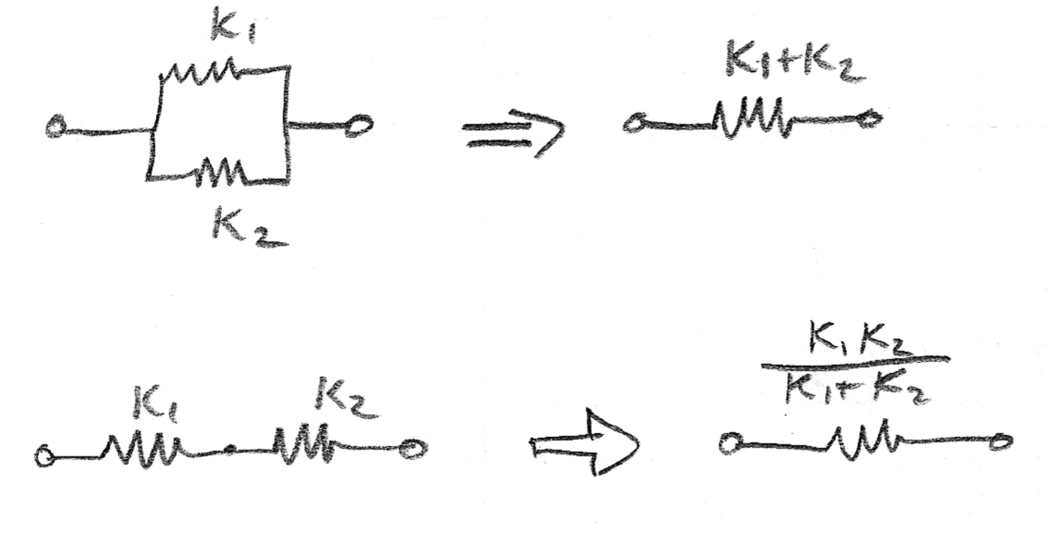
\includegraphics[width=3.5in]{figs02/00723a.png}
\caption{Springs in parallel and series can be combined (like capacitors).}\label{seriessprings}
\end{figure}


\hrule
{\it Proof:}
Consider two springs in series.
The force, $f$ is the same throughout all elements of a serial chain, and both springs independently obey Hooke's Law:

\[
f = K_1\Delta x_1 = K_2\Delta x_2
\]
The total change in length due to the applied force, $f$, is
\[
\Delta x = \Delta x_1 + \Delta x_2
\]

\[
\Delta x = \frac{f}{K_1} + \frac{f}{K_2}
\]

\bq
K_T = \frac{f}{\Delta x} = \frac {1}  {1/K_1 + 1/K_2} = \frac  {K_1K_2} {K_1+K_2}
\eq
\hrule

An almost identical proof can be made for series connected dampers.

However, Mass, $M$ is different (Figure \ref{addtwomasses}) because of the unique property that the force on a mass depends on the acceleration only with respect to the inertial frame:

\[
f = m\ddot{x}, \quad \mathrm{NOT} \quad f = m(\ddot{x}_i - \ddot{x}_j)
\]
Thus


\begin{figure}[h]\centering
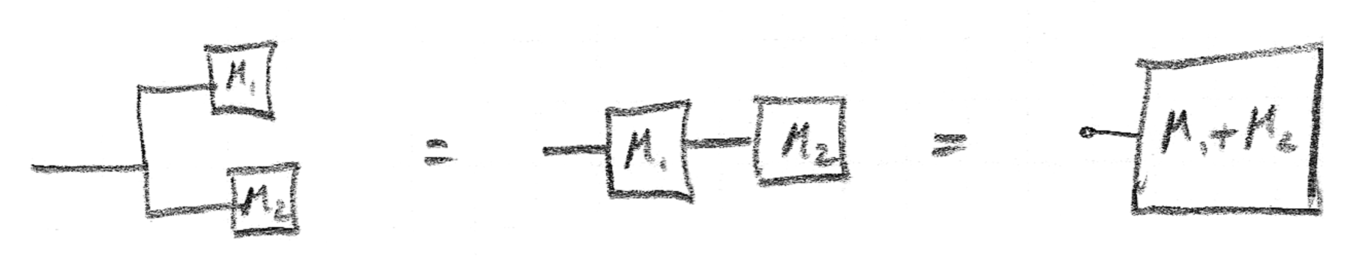
\includegraphics[width=4.5in]{figs02/00724a.png}
\caption{Add two masses which ever way they are combined.}\label{addtwomasses}
\end{figure}

What about the case where a spring and damper are connected in series (Figure \ref{springseriesdamper})?


\begin{figure}\centering
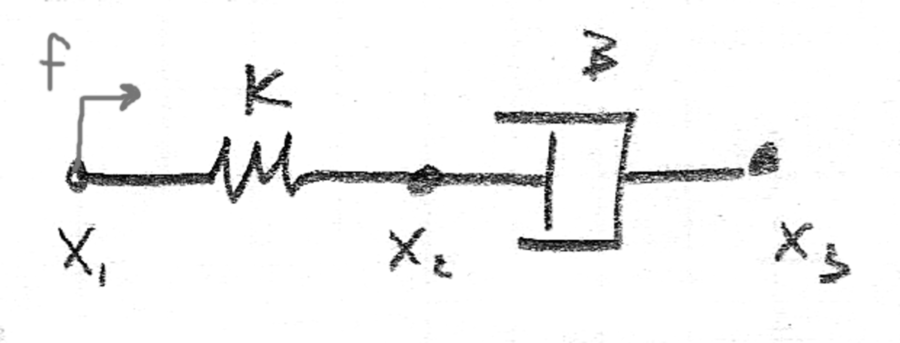
\includegraphics[width=3.0in]{figs02/00725a.png}
\caption{If a spring and damper are connected in series, a new EOM must be constructed for the node in between ($x_2$).}\label{springseriesdamper}
\end{figure}

Using a similar analysis based on the fact that $f$ is the same in both elements of a serial chain:
\[
f = K(x_1-x_2) = B(\dot{x}_2-\dot{x}_3)
\]

The difference here is that we have a new unknown $x_2$.    This new unknown requires a new EOM however $m_2 =0$.   The EOMS for the system of Figure \ref{springseriesdamper} are thus:
\[
K(x_1-x_2) = f
\]
\[
0\ddot{x_2} + K(x_2-x_1) + B(\dot{x}_2-\dot{x}_3) = 0
\]
\[
B(\dot{x}_3-\dot{x}_2) = 0
\]






\subsection{Multiple Masses and EOMs}
When there are multiple independent masses (who's displacements, $x_i$ are not the same) then we need a separate EOM for each mass (Example \thechapter.\ref{MultipleEOMs}).
In a general system with multiple masses, dampers or springs can be connected between any two of the masses.  This is why we used the subscripts and the subtractions in Equation \ref{D'Alembert}.



\begin{ExampleSmall}\label{MultipleEOMs}


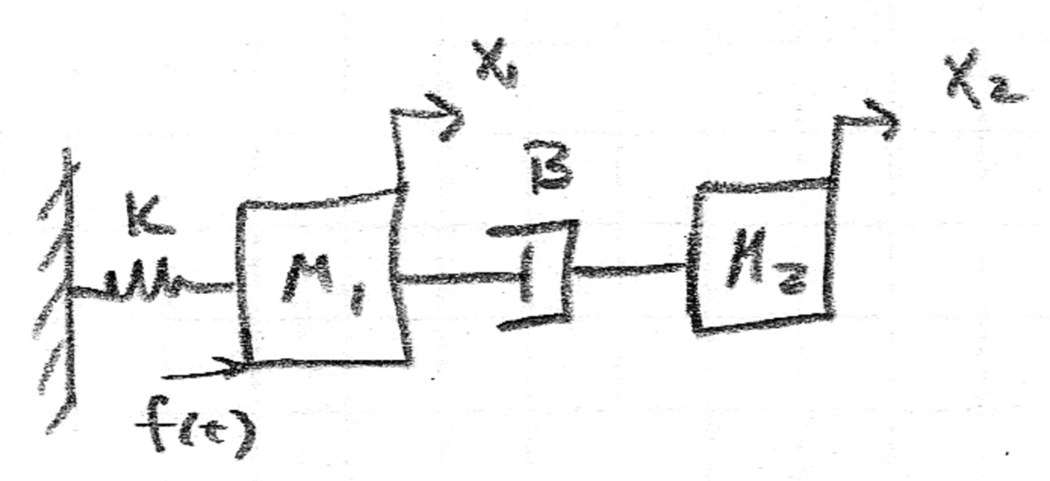
\includegraphics[width=3.5in]{figs02/00726a.png}



By applying Equation \ref{D'Alembert} to each mass,
\[
(M_1) \qquad M_1\ddot{x}_1 + B(\dot{x}_1 - \dot{x}_2) + Kx_1 = f(t)
\]
\[
(M_2) \qquad M_2\ddot{x}_2 + B(\dot{x}_2-\dot{x}_1)  = 0
\]

Note that each EOM for mass $i$ always begins with $M_i\ddot{x}_i$ and that in the $B,K$ terms of EOM$_i$, $x_i$ is always taken positive.
\end{ExampleSmall}





\section{Conversion to Transfer Function}

EOMs are {\it Linear Ordinary Differential Equations}, LODEs.  As such, we can easily apply the Laplace Transform.
Using the EOMs of Example \thechapter.\ref{MultipleEOMs},
\[
M_1X_1(s)s^2 + BX_1(s)s - BX_2(s)s + KX_1(s) = F(s)
\]
\[
M_2X_2(s)s^2 + BX_2(s)s - BX_1(s)s = 0
\]
Note that we have assumed zero initial conditions.   What does this assumption mean?  Mathematically it means
\[
x_i(t=0) = 0, \quad \dot{x}_i(t=0) = 0, \quad \ddot{x}_i(t=0) = 0
\]
and physically this corresponds to the system being at rest and having no kinetic or potential energy.

We will use the Laplace transform to solve for a {\it Transfer Function}.   Transfer functions are ratios between the Laplace Transforms of two physical variables.  Examples:

\[
\frac{X_2(s)}{F(s)} \qquad
\frac{X_1(s)}{X_2(s)} \qquad \mathrm{etc.}
\]

Often we need to analyze a system when we know its input (say $X(s)$) but do not know its output (say $Y(s)$).  If we can obtain the transfer function
\[
G(s) = \frac{Y(s)}{X(s)}
\]

then we can get the Laplace transform of the output by
\[
Y(s) = G(s)X(s)
\]

The transfer function is obtained by algebraically manipulating the Laplace transform of one or more EOMs.
Sometimes multiple EOMs have to be solved simultaneously to get the transfer function.

\begin{ExampleSmall}\label{TransferFunctionExample}
For the system of Example \thechapter.\ref{example2dampers}, let's find the transfer function
\[
G(s) = \frac {X(s)}{F(s)}
\]
Using this transfer function we could compute the displacement as a function of the input force.


There is only one mass and thus only one EOM.  Starting with the EOM

\[
M\ddot{x} + (B_1+B_2)\dot{x}+Kx = f(t)
\]

First take the Laplace Transform:
\[
(LT) \qquad   MX(s)s^2 + (B_1+B_2)X(s)s + KX(s) = F(s)
\]
then we factor out $X(s)$ from each term giving
\[
X(s)\left( Ms^2 +(B_1+B_2)s + K \right) = F(s)
\]
dividing through we get the transfer function
\[
G(s) = \frac {X(s)}{F(s)} = \frac {1}{Ms^2 + (B_1+B_2)s + K }
\]

\end{ExampleSmall}


We will find it useful to {\it normalize} each transfer function before further analysis.   This means that we will manipulate each polynomial in $s$ so that the coefficient of  highest power of $s$ is 1\footnote{Known as a ''monic" polynomial.}.    This is accomplished by just dividing through by the coefficient of the highest power of $s$ as a final step.


\begin{ExampleSmall}
Normalize the transfer function of Example \thechapter.\ref{TransferFunctionExample}.

Dividing through top and bottom by $M$,

\[
G(s) = \frac {X(s)}{F(s)} = \frac {1/M}{s^2 + \frac{B_1+B_2}{M}s + \frac{K}{M} }
\]
\end{ExampleSmall}


\section{Examples}

%%%%%%%%%%%%%%%%%%%%%%%%%%%%%%%%%%%%%%%%%%%%%%%%%%%%%%%%%%%%%%%%%%%%%%%%%%%%%%%%%%%%%%%%%%%%%%%%%%%%%%%%%
\begin{Example}\label{3MassExample}
Two sliding masses.


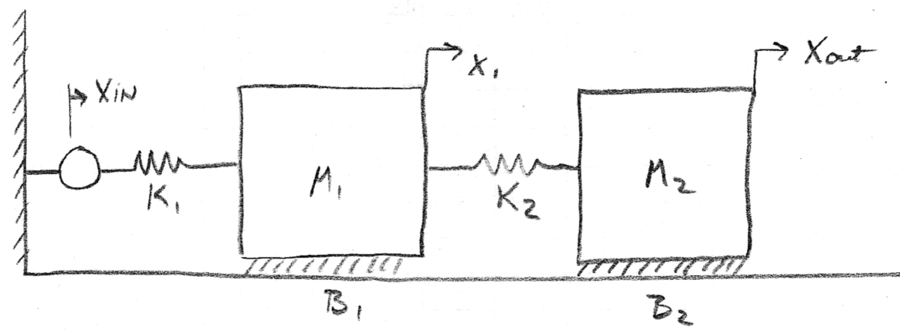
\includegraphics[width=3.0in]{figs02/00727a.png}

(Note that in this diagram, we used hatching between the mass and ground to indicate damping ($B_1, B_2$).  This symbol is commonly used because it visually suggests sliding friction.

Find
\[
G(s) = \frac{X_{out}(s)}{X_{in}(s)}
\]
Normalize the Denominator of the solution.

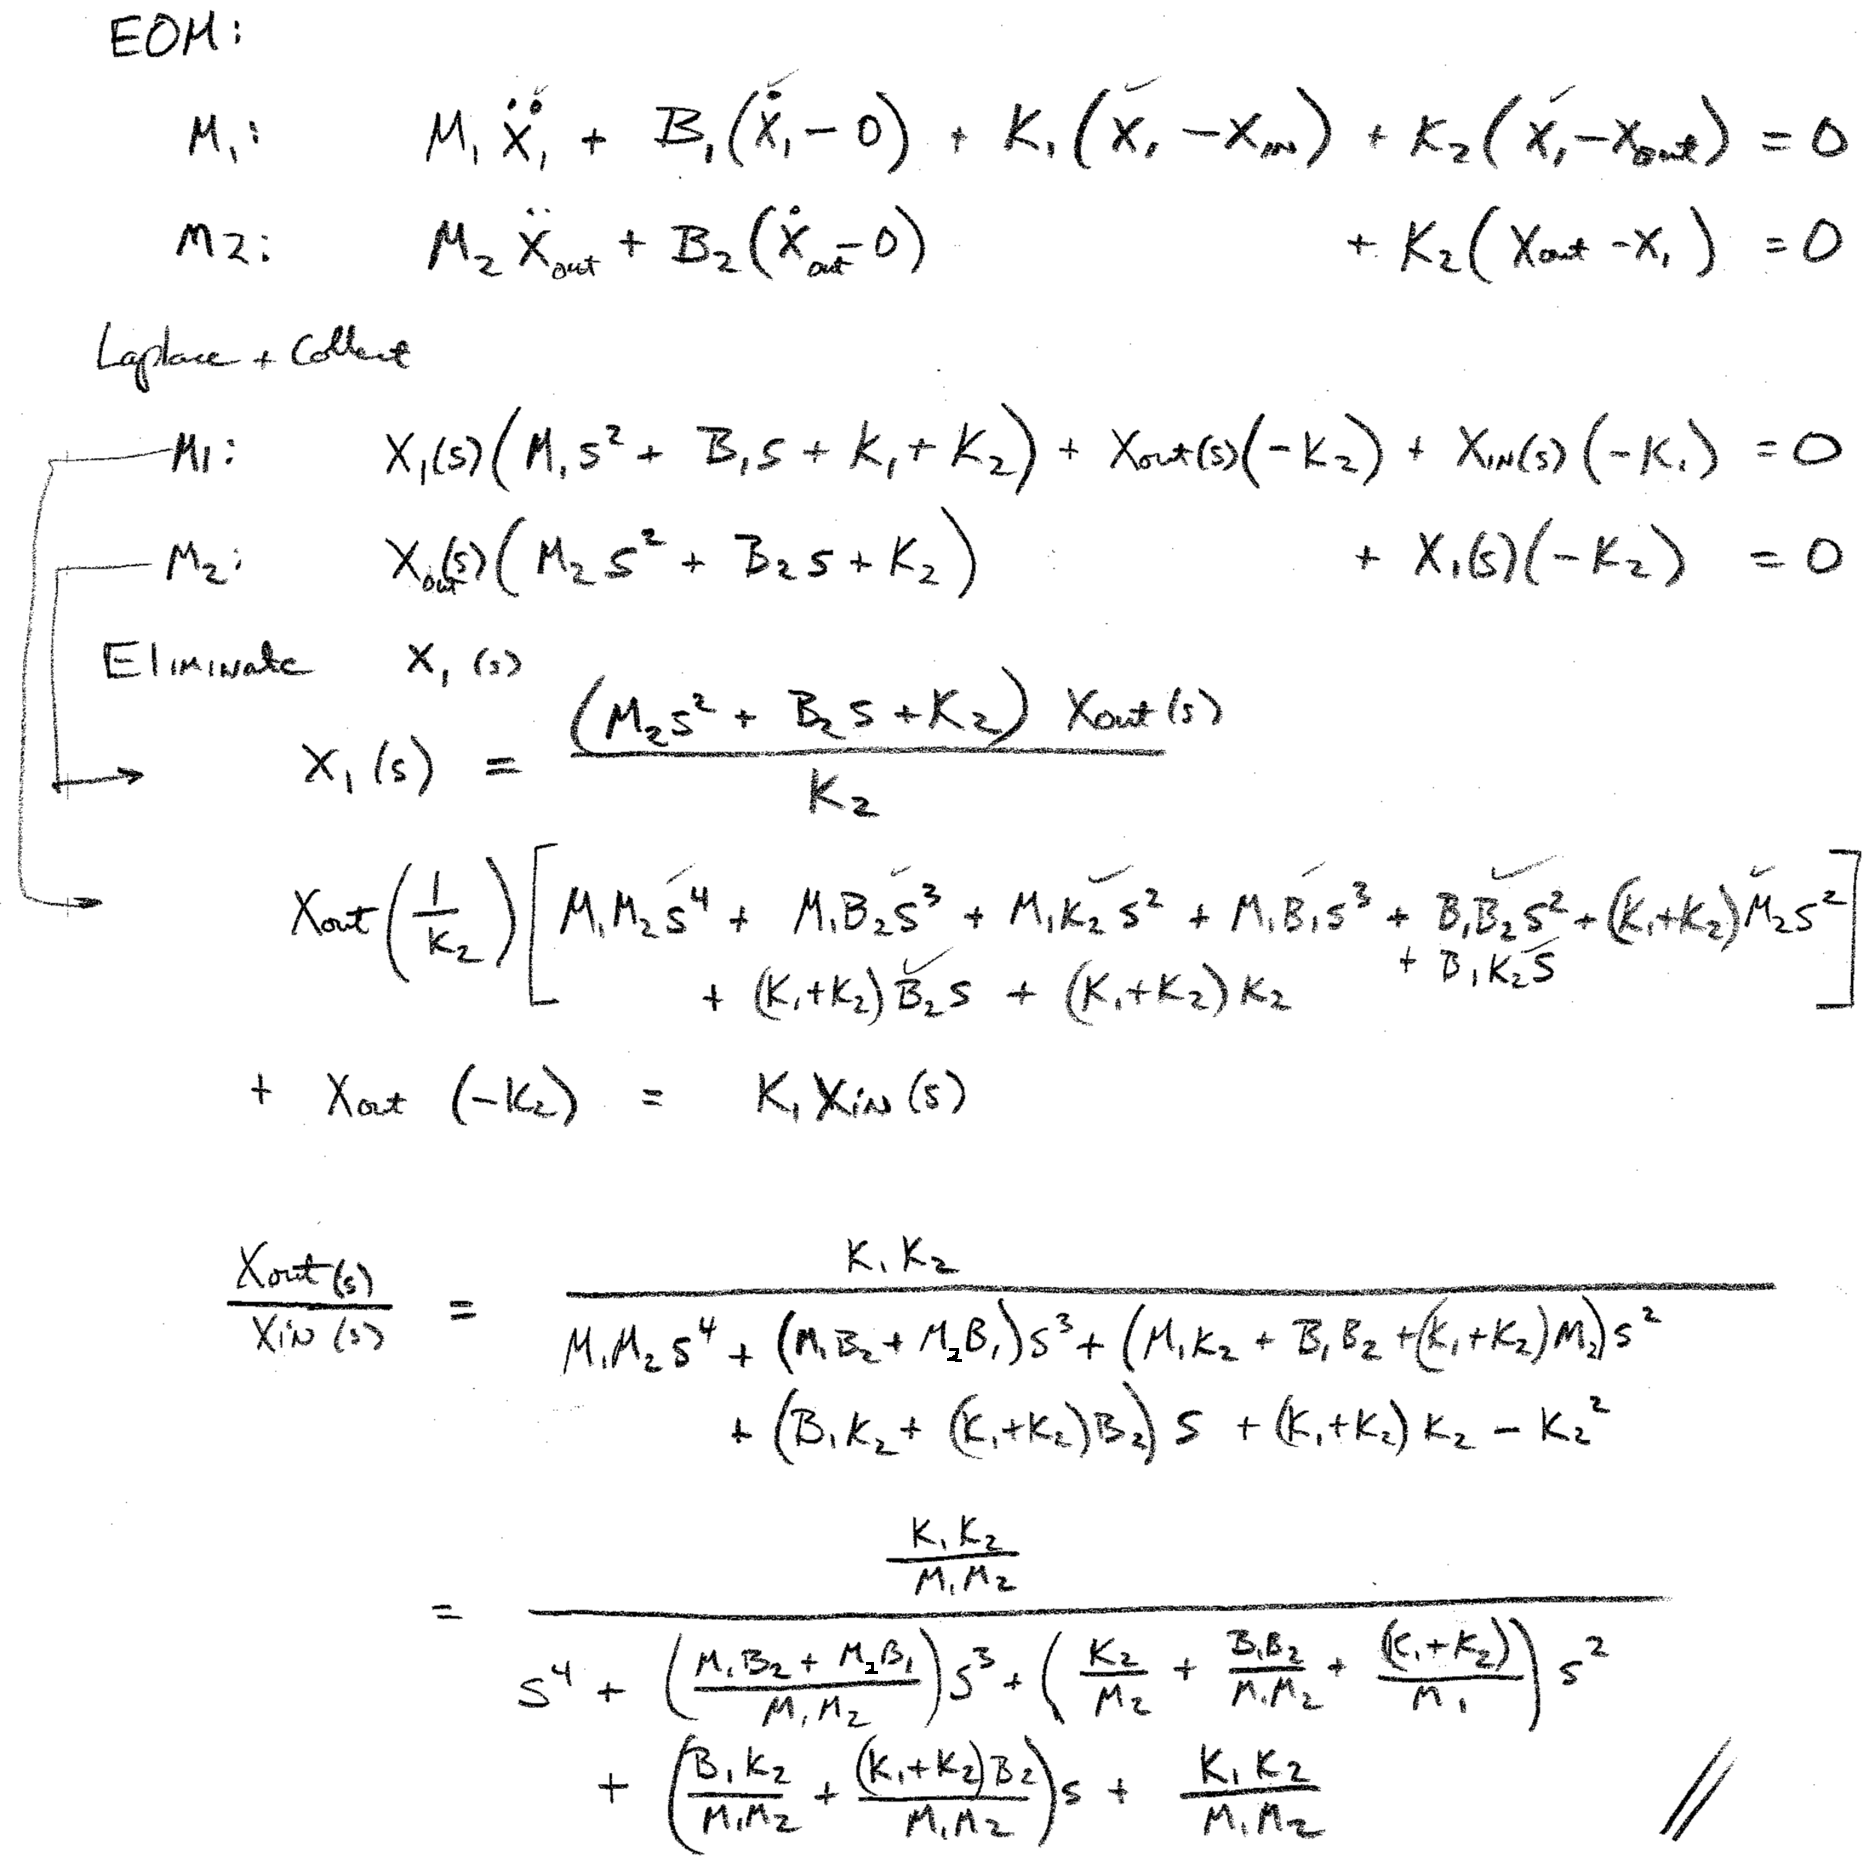
\includegraphics[width=6.25in]{figs02/00729a.png}

\end{Example}



%%%%%%%%%%%%%%%%%%%%%%%%%%%%%%%%%%%%%%%%%%%%%%%%%%%%%%%%%%%%%%%%%%%%%%%%%%%%%%%%%%%%%%%%%%%%%%%%%%%%%%%%%

\begin{Example}\label{ExampleCarSuspensionTF}   %2.8
Car Suspension Example

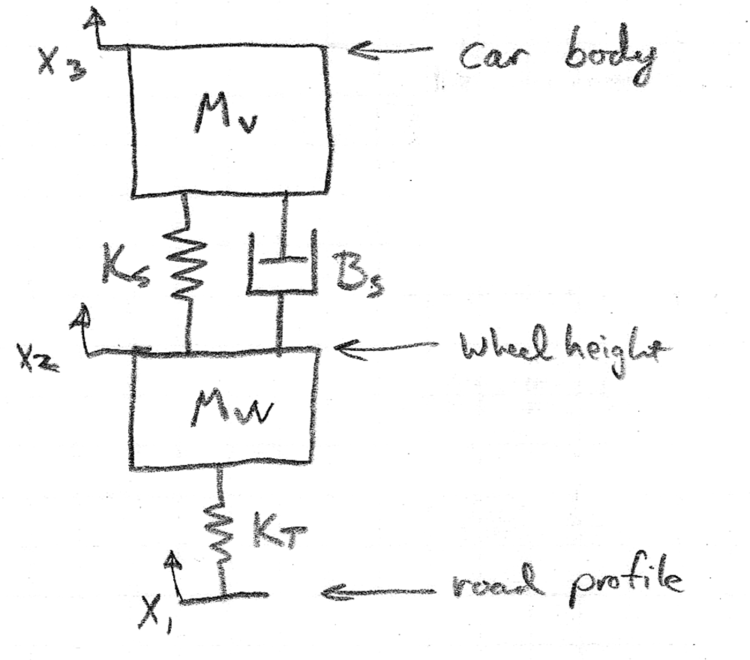
\includegraphics[width=2.5in]{figs02/00730a.png}    Find the transfer function from road ($x_1(s)$) to body ($x_3(s)$).
Normalize the denominator.


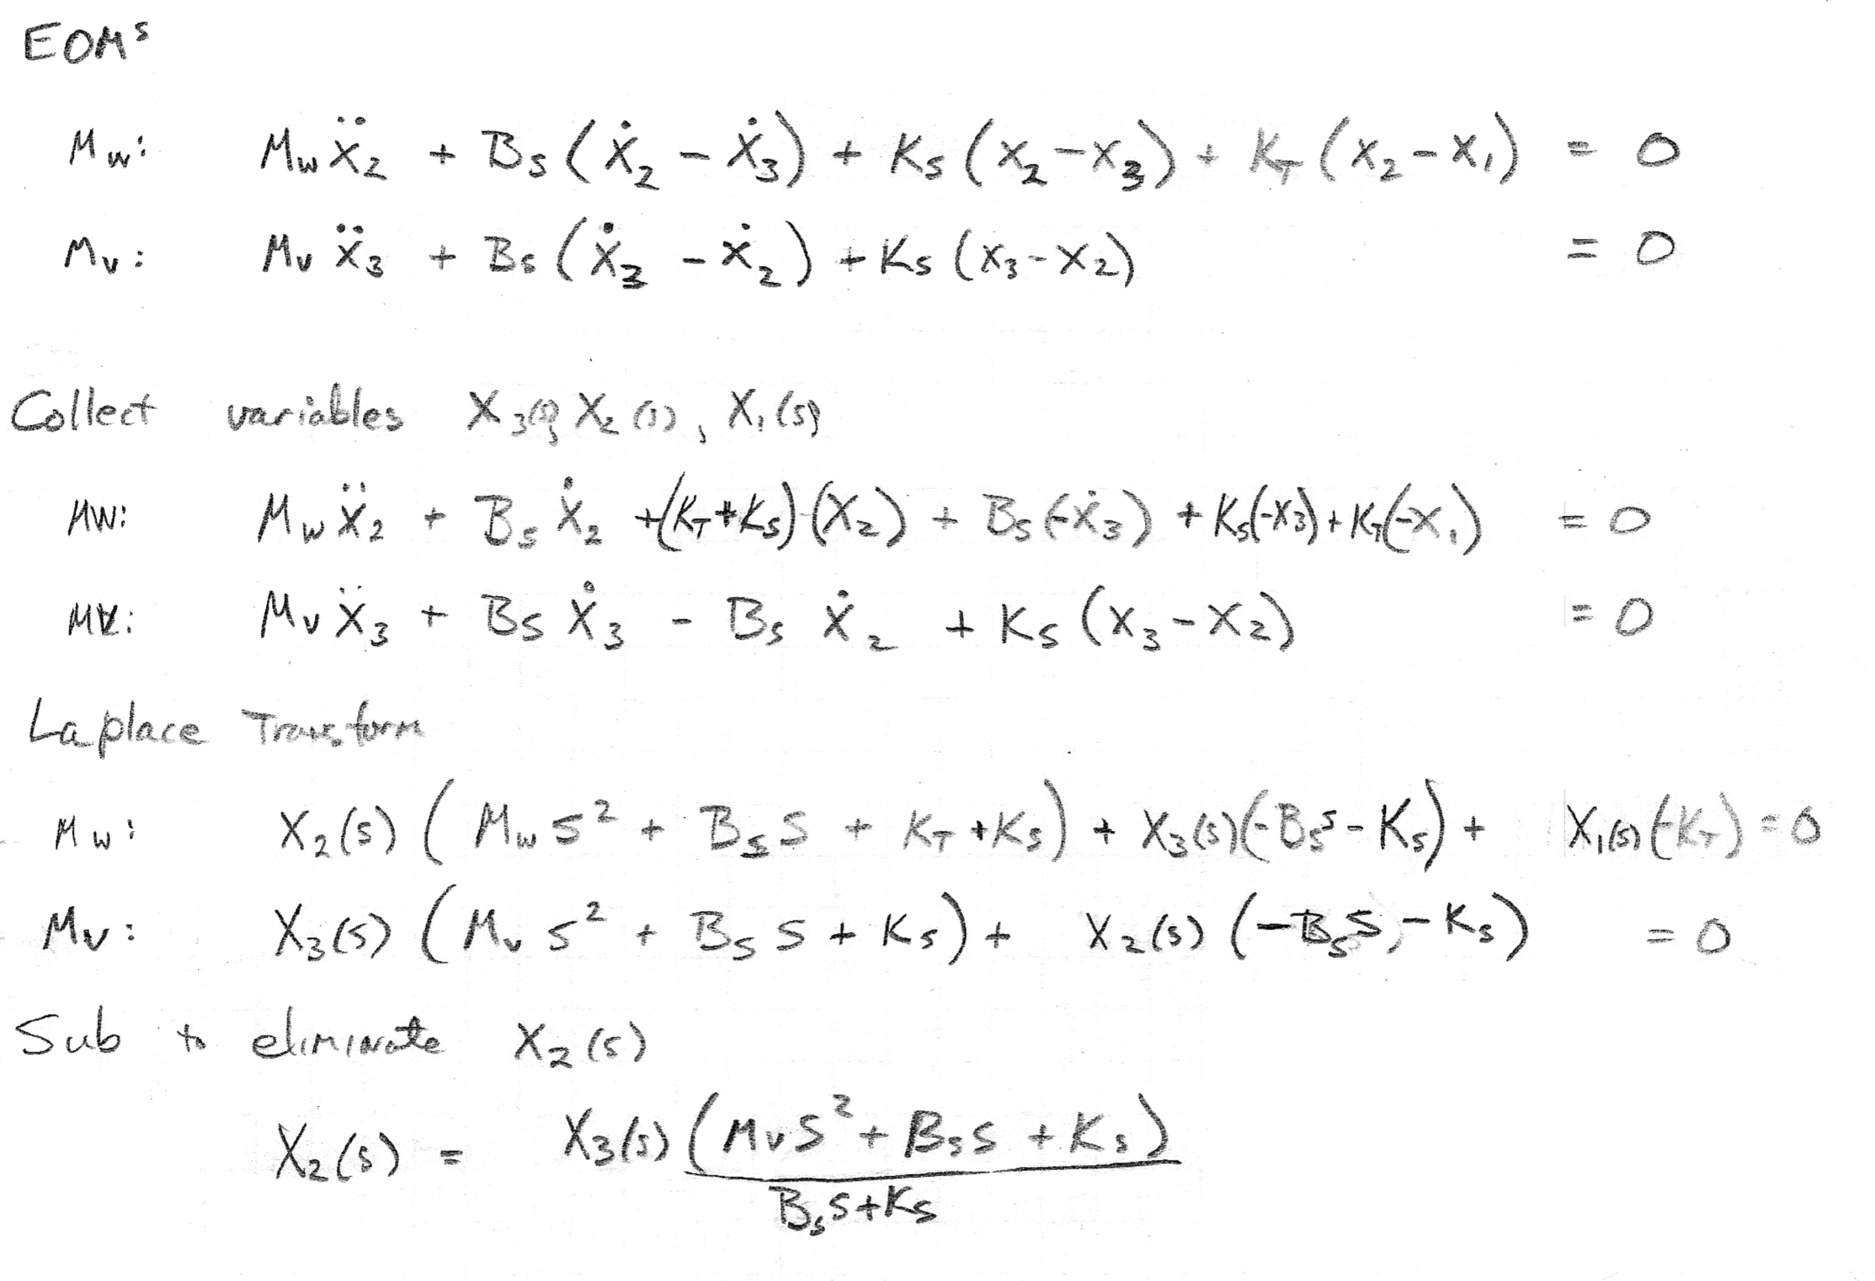
\includegraphics[width=6.25in]{figs02/00731a.png}

\end{Example}

%
\begin{ExampleCont}
  %
Note what we have done under ``Collect Variables" above is to simply collect terms according to the motion variables in a systematic
way.  Specifically we can stay organized by filling
out a table re-arranging the EOMs as follows:\vspace{0.3in}



% Make table rows deeper
\renewcommand\arraystretch{1.5}% Vertical Row size, 1.0 is for standard spacing)


\begin{tabular}{|p{0.35in}|p{0.55in}|p{0.55in}|p{0.55in}|p{0.35in}|p{0.65in}|p{0.55in}|p{0.55in}|p{0.35in}|}\hline
  Eqn\# & $\ddot{x_j}$ & $\dot{x_1}$ & $x_1$  & $\dot{x_2}$ & ${x_2} $& $\dot{x_3}$ & ${x_3} $ &  = \\ \hline
  (1)   & $M_w\ddot{x}_2$ & 0 & $(-K_T)$ & $B_S$    & $(K_T+K_S)$ & $(-B_S)$ & $(-K_S)$ & 0  \\ \hline
  (2)   & $M_v\ddot{x}_3$ & 0 & 0        & $(-B_S)$ & $(-K_S)$    & $B_S$    & $K_S$    & 0 \\ \hline
\end{tabular}

Note that our system equations seem to lack an input (which would be on the right-hand-side i.e. the
last column of our tabular form).  Thinking back to cars, the input would be changes in road height,
$x_1$ (which is not attached to a mass).  We can thus re-do the table to move $x_1$ terms to
the right hand side:

\begin{tabular}{|p{0.35in}|p{0.55in}|p{0.55in}|p{0.55in}|p{0.35in}|p{0.65in}|p{0.55in}|p{0.55in}|p{0.35in}|}\hline
  Eqn\# & $\ddot{x_j}$ & $\dot{x_1}$ & $x_1$  & $\dot{x_2}$ & ${x_2} $& $\dot{x_3}$ & ${x_3} $ &  = \\ \hline
  (1)   & $M_w\ddot{x}_2$ & 0 & $0$ & $B_S$    & $(K_T+K_S)$ & $(-B_S)$ & $(-K_S)$ & $K_Tx_1$ \\ \hline
  (2)   & $M_v\ddot{x}_3$ & 0 & 0        & $(-B_S)$ & $(-K_S)$    & $B_S$    & $K_S$    & 0 \\ \hline
\end{tabular}

This tabular method will be useful later when we derive state space system equations.

Getting back to the transfer function:

%  \includegraphics[width=6.25in]{figs02/00961a.png}
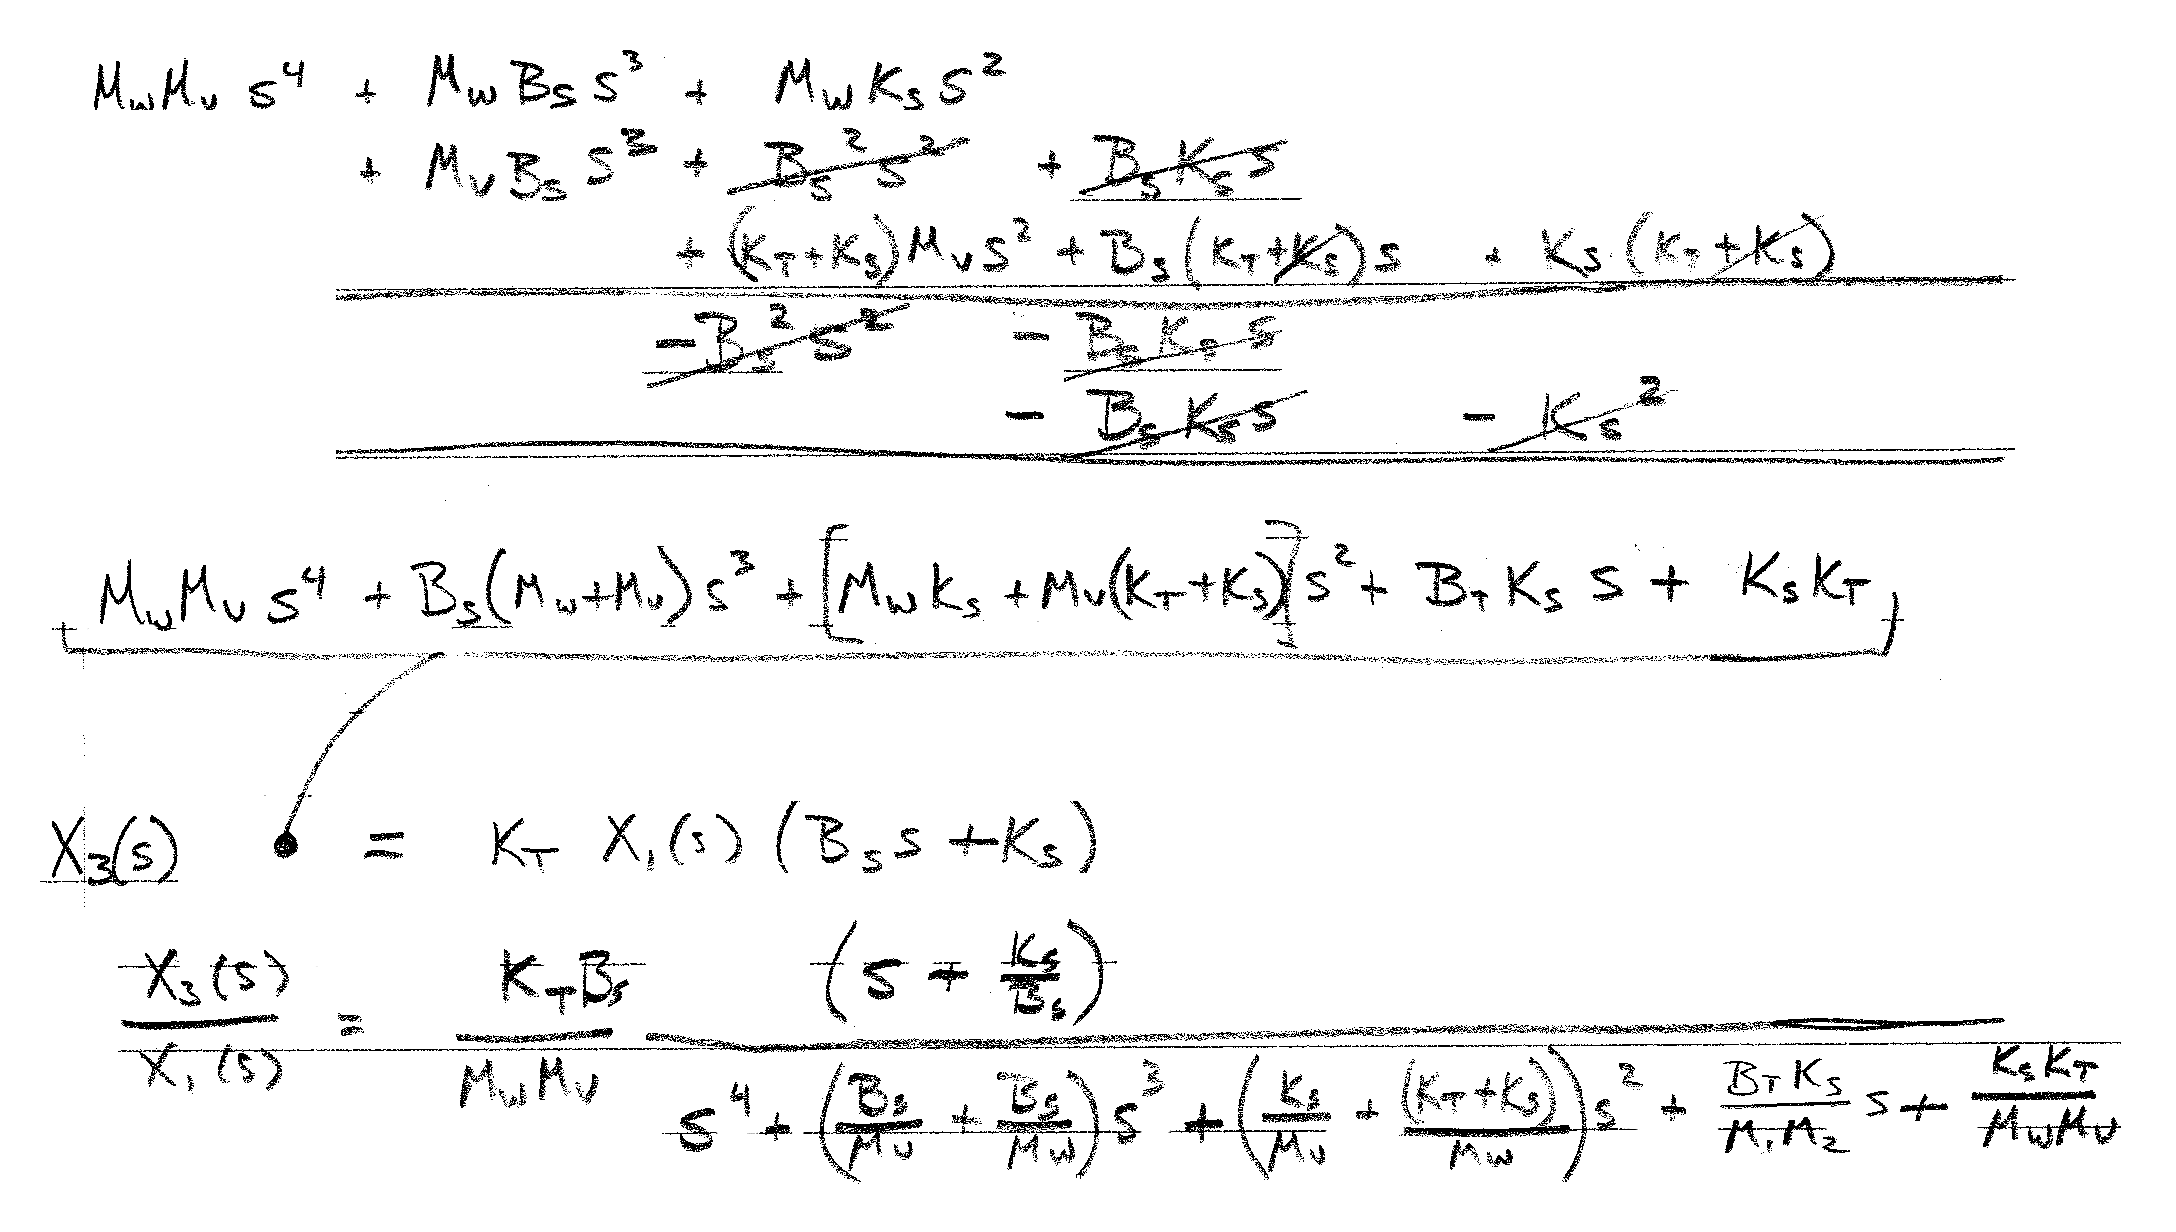
\includegraphics[width=6.0in]{figs02/00961.png}

\end{ExampleCont}



\section{Finding Errors through Dimensional Analysis}

Once the numerator and denominator of the transfer function are normalized, we can exploit dimensional analysis to check our work for errors.   We rely on the fact that for quantities to be added together they must have the same units.  What are the units of $s$?

$s$ represents frequency and so has the units of inverse seconds, $\mathrm{sec}^{-1}$.  Also each physical parameter has units.  The MKS system has only three {\it fundamental units}, meters, kg, and seconds. Assuming the MKS system, each physical parameter has the units given in Table \ref{unitstable}.

\begin{table}[h]\centering
\renewcommand{\arraystretch}{1.5} %<- modify value to suit your needs
\begin{tabular}{c|l||c|l}
Name	& Fundamental Units & Name	& Fundamental Units \\ \hline
$s$	& $\mathrm{sec}^{-1}$      & $B$	& $\frac{kg}{\mathrm{sec}}$  \\
$s^n$   & $\mathrm{sec}^{-n}$  & $K$	& $\frac{kg}{\mathrm{sec}^2}$  \\
& & $M$	& $kg$ \\
\end{tabular}
\caption{Fundamental MKS units for $s$ and the physical parameters.}\label{unitstable}
\end{table}

Now suppose the denominator of a transfer function has been normalized and then begins with $s^4$.   Then through dimensional analysis, we know that all the subsequent terms in the polynomial must have the same units, namely sec$^{-4}$.  This can often be an easy way to find an error in the transfer function without checking each step. Note that you can also apply this to the tabular version of
Example 2.\ref{ExampleCarSuspensionTF}
by making sure all entries in each column have the same units.




\begin{Example}\label{DimensionalAnalysisExample}

We have derived the following transfer function:

\[
G(s) = \left( \frac {B} {M_1M_2}\right) \frac{s+K/M}
 {s^4 + \frac{M_1+M_2}{M_1M_2}Bs^3+(1/M_1+1/M_2)2BKs^2+\frac{2BK}{M_1M_2}s+\frac{3K^2}{M_1M_2}}
\]

Check for errors using dimensional analysis:
We  ignore the normalizing term $\frac{B}{M_1M_2}$ because it is outside the additions.  It could be right or wrong, but
dimensional analysis won't help us with this particular term.


{\bf Numerator:}
\[
s+K/M
\]
First, we have $s$.  The units of $s$ are sec$^{-1}$.  Checking the next term $\frac{K}{M}$, we convert each term into its fundamental units and multiply them:

\begin{tabular}{c|c|c}
$K$ 	&	$1/M$  &	\\ \hline
$\frac{kg}{\mathrm{sec}^2}$ & $1/kg$ & $= \frac{1}{\mathrm{sec}^2} \neq \mathrm{sec}^{-1}$ \\
\end{tabular}

The units do not agree with sec$^{-1}$ so this is an \hspace{0.25in}  {\bf ERROR!}


\vspace{0.15in}

{\bf Denominator: }
\vspace{0.2in}
The first term is $s^4$.  Therefore, all terms in demoninator must have net units of $\mathrm{sec}^{-4}$.  The next term is
\[
\frac{M_1+M_2}{M_1M_2}Bs^3
\]
In the $\frac{M_1+M_2}{M_1M_2}$ term, the units reduce to $1/M$ by cancellation.   Therefore we can break it down as

\begin{tabular}{c|c|c|c}
$1/M$	& $B$      & $s^3$ & \\ \hline
$1/kg$  & $kg/sec$ & $\mathrm{sec}^{-3}$ & $= \mathrm{sec}^{-4}$
\end{tabular}
\hspace{0.25in}  {\bf CORRECT}



Continuing in this manner:
\[
(1/M_1+1/M_2)2BKs^2
\]

\begin{tabular}{c|c|c|c|c}
$1/M$	& $2B$	& $K$	& $s^2$ & \\ \hline
$1/kg$  & $kg/\mathrm{sec}$	& $kg/\mathrm{sec}^2$	& $1/\mathrm{sec}^2$	& $= \frac{kg}{\mathrm{sec}^5} \neq \mathrm{sec}^{-4}$
\end{tabular}
\hspace{0.25in}{\bf ERROR!}


\[
\frac{2BK}{M_1M_2}s
\]


\begin{tabular}{c|c|c|c|c}
$1/M^2$	  & $2B$		& $K$	& $s$ & \\ \hline
$1/kg^2$  & $kg/\mathrm{sec}$	& $kg/\mathrm{sec}^2$	& $1/\mathrm{sec}$	& $= \frac{1}{\mathrm{sec}^4} = \mathrm{sec}^{-4}$
\end{tabular}
\hspace{0.25in}  {\bf CORRECT}



\[
\frac{3K^2}{M_1M_2}
\]

\begin{tabular}{c|c|c}
$1/M^2$	& $3K^2$   & \\ \hline
$1/kg^2$  & $kg^2/\mathrm{sec}^4$	& $= \frac{1}{\mathrm{sec}^4} = \mathrm{sec}^{-4}$
\end{tabular}\hspace{0.25in}  {\bf CORRECT}

\end{Example}

\section{More complex problems}
The structure we have added to the EOMs in Example 2.\ref{ExampleCarSuspensionTF}, as well as the
use of dimensional analysis for easy debugging of your equations, makes it easier than you
might expect to analyze a more complex system (or break a system down into a more detailed model).
For example, let's write down equations of motion for a kind of intimidating
system with 4 masses and many springs and
dampers as in Figure \ref{complexDynSystem}.


\begin{figure}\centering
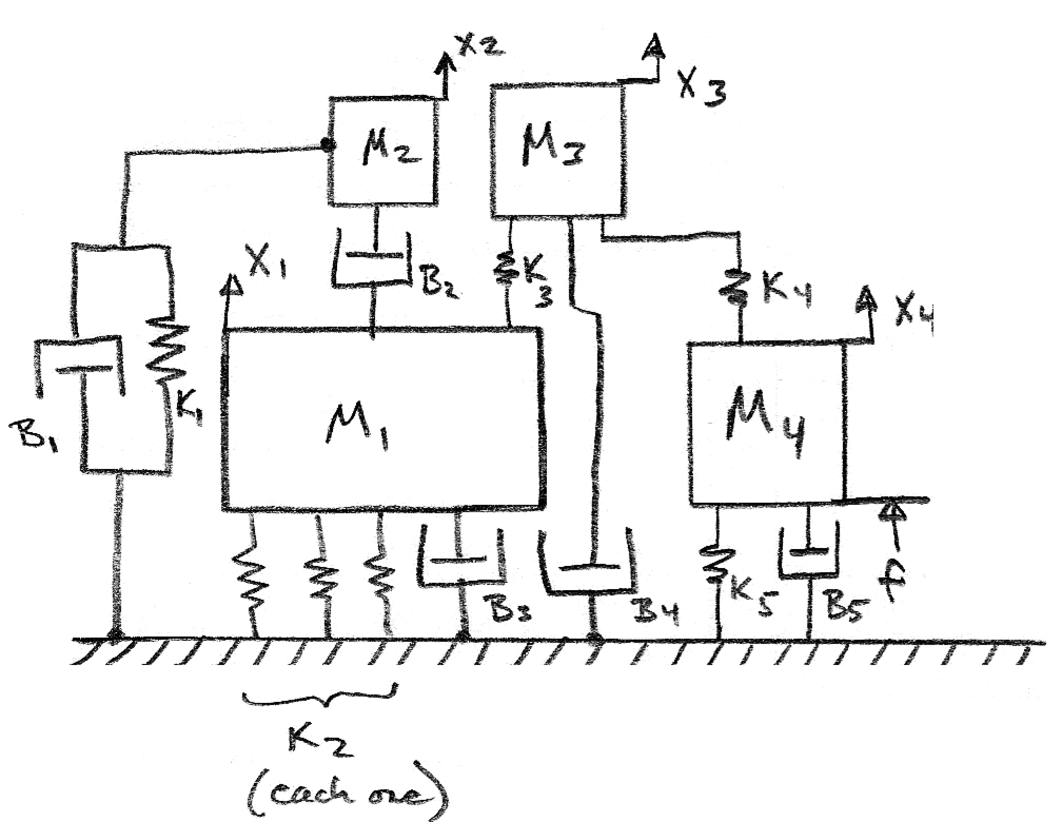
\includegraphics[width=90mm]{figs02/00933a.png}
\caption{A system with 4 masses and numerous springs and dampers connecting them.}
\label{complexDynSystem}
\end{figure}

\begin{Example}
  Write the 4 EOMs for the system of Figure \ref{complexDynSystem}.

Summing forces on each mass:
\[
M_1\ddot{x}_1 + B_3\dot{x}_1+B_2(\dot{x}_1-\dot{x}_2) +3K_2x_1+K_3(x_1-x_3)  = 0
\]
\[
M_2\ddot{x}_2 + B_2(\dot{x}_2-\dot{x}_1)+B_1\dot{x}_2+K_1x_2 = 0
\]
\[
M_3\ddot{x}_3 + B_4\dot{x}_3+K_3(x_3-x_1)+K_4(x_3-x_4)=0
\]
\[
M_4\ddot{x}_4+B_5\dot{x}_4+K_4(x_4-x_3)+k_5x_4 = f(t)
\]


Now re-organize the equations into tabular form as above (but changing to a vertical table).   Each equation (column) is a sum and each row is the coefficient of
each variable in the first column.

\begin{tabular}{|c|c|c|c|c|c|}\hline
  Var           & EOM1 & EOM2 & EOM3 & EOM4\\\hline
  $M_j\ddot{x}_j$  & $M_1\ddot{x}_1$&$M_2\ddot{x}_2$&$M_3\ddot{x}_3$ &$M_4\ddot{x}_4$ \\ \hline
  $\dot{x}_1$   & $(B_2+B_3)$ &$(-B_2)$  & 0           & 0 \\ \hline
        $x_1$   & $(3K_2+K3)$ &0         & 0           & 0 \\ \hline
  $\dot{x}_2$   & $-B_2$      & $B_2$    & 0           & 0 \\ \hline
        $x_2$   & 0           & $K_1$    & 0           & 0 \\ \hline
  $\dot{x}_3$   & 0           & 0        & $B_3$       & 0 \\ \hline
        $x_3$   & $(-K_3)$    & 0        & $(K_3+K_4)$ & $(-K_4)$ \\ \hline
  $\dot{x}_4$   & 0           & 0        & 0           & $B_5$    \\ \hline
        $x_4$   & 0           & 0        & $(-K_4)$    & $(K_4+K_5)$ \\ \hline\hline
        =       & 0  & 0  & 0 & $f(t)$ \\ \hline
\end{tabular}


Remember, each vertical column is an equation.  the last line is the right
hand side and the first 9 lines are added to form the right hand side.
Taking the first column as an example:
\[
M_1\ddot{x}_1+(B_2+B_3)\dot{x}_1+(3K_2+K_3)x_1-B_2\dot{x}_2 -K_3x_3 = 0
\]

\end{Example}

Although it is sometimes possible to derive useful transfer functions from
this point, systems of this complexity have many possible transfer functions
(based on selecting different input and output points).
Arranging a complex
system into tabular form like this makes it simple to transition to
the matrix-based State Space form which we will introduce in Chapter
\ref{BasicsStateSpaceChapter}.

Also, let's check our work.   First, since each equation is 2nd order
and $\dot{x} \to sX(s), \; x \to X(s)$, then each row must have the same
units in cols 2-5.   Also all the ``dot'' rows must have $B$ units
and all the $x_j$ rows must have $K$ units.   By these rules  our work
above checks out (but remember, it still could contain some errors!).

Finally,  we used the column form here
to fit on the page but the row form (as in Example
2.\ref{ExampleCarSuspensionTF}) will be a closer match to the matrix equations
we will use.
   % Translational Dynamics
% %
%
%


\chapter{Rotational Dynamical Systems}

%%%%** Section 1
\section{Problem Statement and Learning Objectives}
Be able to
\begin{itemize}
  \item Name system elements, write, and graph constitutive relations for the basic elements
  of a rotational mechanical system.
  \item Write the Equations of Motion for a rotational system with any number of masses, springs, and dampers.
  \item Write EOMs for rotational systems containing gears
\end{itemize}

%%%%** Section 2
\section{System Elements \& constitutive relations.}

Rotation is a different type of motion than translation which  makes subtle differences in dynamic analysis.   One of the most prominent differences is that if a body is rotating, every point in the body has a different velocity and acceleration.   This complex situation can be considerably simplified by assuming a single axis of rotation, and representing a body by its {\it inertia} instead of its mass.   The axis of rotation is a line along which points in a rigid body do not move when it is rotated.

Computation of the inertia of a rigid body is beyond the scope of this book, but it is a quantity which can be measured by rotational tests, or calculated from information such as a CAD model.

%%%%** Section 2.1
\subsection{Torque}

{\it Torque} (also called {\it moment}) is a vector quantity relating a force and an associated {\it moment arm} through which the force acts to rotate a body around an axis.   The simplest case is a force which is perpendicular to both the axis of rotation and a radius connecting the axis and the point through which the force is acting on the rigid body (Figure \ref{forceradisutorque}, Left). In this case, the magnitude of the torque is
\[
|\tau| = |r||F|
\]
and the full magnitude and direction of the torque vector will be obtained by the right hand rule
\[
\tau = r \times F
\]
(where $\times$ indicates the vector cross product).

If the force vector is not applied at a right angle (Figure \ref{forceradisutorque}, Right), it must be resolved into  perpendicular and radial components, $F_p, F_r$, and then the torque magnitude is
\[
|\tau| = |r||F_p|
\]
the full torque vector can still be obtained by the vector cross product above.   When the axis of rotation is fixed, for example by a shaft mounted in bearings, then only the component of the torque vector which is parallel to the axis causes rotation about the axis.

In most of the problems we will study however, we will assume that a torque value is a known or measured quantity and not worry about the radius or moment arm.  In a very common control system application, a DC electric motor is applied to a shaft and the torque is simply proportional to the current
\[
\tau(t) = K_m i(t)
\]

%%%%** Figure 1
\begin{figure}\centering
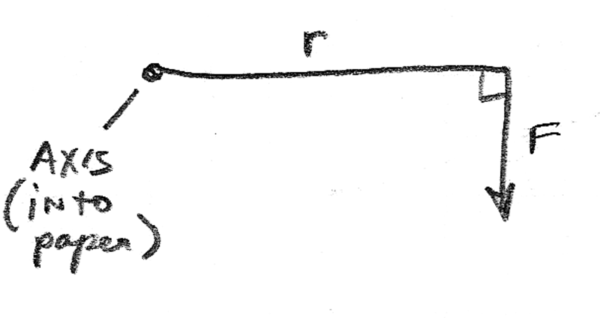
\includegraphics[width=2.0in]{figs03/00749a.png} \hspace{0.75in}
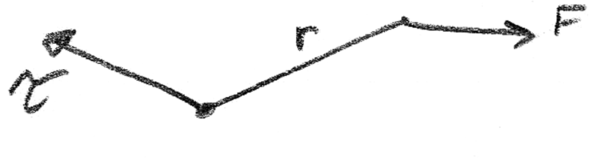
\includegraphics[width=2.0in]{figs03/00750a.png}
\caption{An applied force $F$ generates a torque if it acts through a point having a radius, $r$ from the axis of rotation. Left: force is applied perpendicular to the moment arm. Right: force is appled in a general direction. (see text).}\label{forceradisutorque}
\end{figure}


















%%%%** Section 2.2
\subsection{Elements of Rotational Dynamical Systems}
We will analyze systems consisting of
\begin{itemize}
  \item {\bf Inertia}     The property of a rigid body which resists angular acceleration, and which stores kinetic energy.
  \item {\bf Stiffness}   The property of a rigid body which resists angular displacement, and which stores potential energy.
  \item {\bf Damping}     The property of a rigid body which resists change in angular displacement and which converts motion to heat.
\end{itemize}


Some properties of the various elements are summarized Table \ref{RotElementsTable}.


%%%%** Table 1
\begin{table}
\begin{tabular}{|l|l|l|l|p{2.0in}|} \hline
 Name             &  Physical Realization      &   Symbol    &  Equation              & Units and Notes   \\ \hline
  Inertia         &  Flywheel                    &   $J$ \raisebox{-\totalheight}{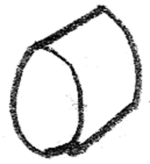
\includegraphics[width=0.5in]{figs03/00740aa.png}}    &  $\tau(t) = J\ddot{\theta}$   & $kg\; m^2$  \\ \hline
  Stiffness       &  Coil  Spring                &   $K$ \raisebox{-\totalheight}{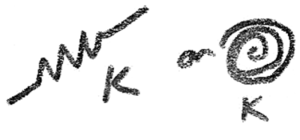
\includegraphics[width=1.0in]{figs03/00740ba.png}}   &  $\tau(t) = K{\theta}$         & $N\; m\; rad^{-1}$, $\tau$ is same on both sides.  Assume zero rest length \\ \hline
  Damping         & Fan, rotary damper, friction &   $B$ \raisebox{-\totalheight}{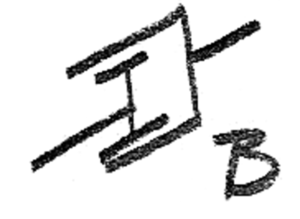
\includegraphics[width=1.0in]{figs03/00740ca.png}}   &  $\tau(t) = B\dot{\theta}$     & $N\; m\;sec^{-1}\;rad^{-1}$, This is a linear model for friction.     \\ \hline
\end{tabular}\caption{}\label{RotElementsTable}
\end{table}



%%%%** Section 3
\section{Equations of Motion}
Similarly to translational motion (see Equation \ref{D'Alembert}), there is an Equation of Motion (EOM) for each inertia in the system:
\[
J\ddot{\theta} + \sum_j B_j(\dot{\theta} -\dot{\theta}_j) + \sum_kK(\theta-\theta_k)
\]

The use of this EOM is similar to that of translational dynamical systems as illustrated in the following examples

\begin{ExampleSmall}
Find the equation or equations of motion for the following system

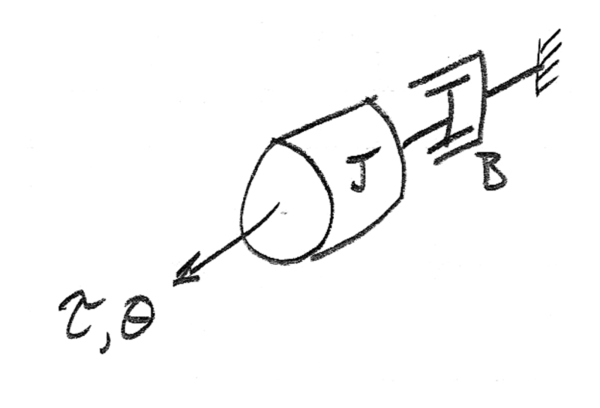
\includegraphics[width=2.0in]{figs03/00741a.png}

There is one inertia ($J$) so there is only one EOM:
\[
J\ddot{\theta} + B(\dot{\theta}-0) = \tau(t)
\]
or
\[
J\ddot{\theta} + B\dot{\theta} = \tau(t)
\]
\end{ExampleSmall}


\begin{ExampleSmall}
Find the equation or equations of motion for the following system

\begin{tabular}{p{2.5in}p{3.25in}}
\vtop{\vskip-2ex \hbox{ 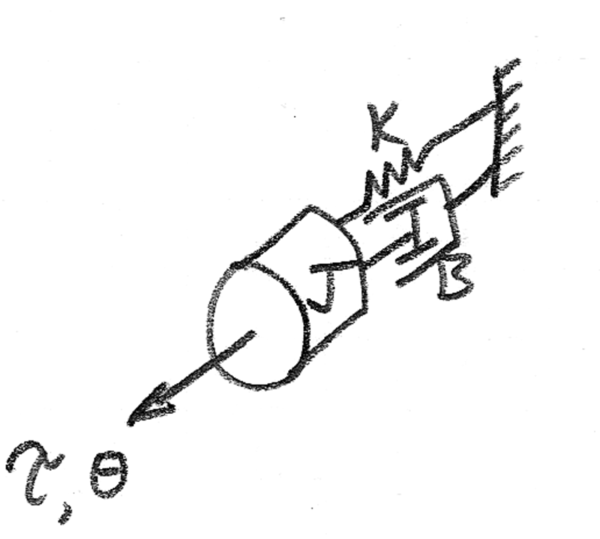
\includegraphics[width=2.0in]{figs03/00742a.png}  }} &
\vspace{0.25in}
(Note: the schematic looks non-physical in this example (``do the damper and spring get wound around each other?''))
but is just a schematic representation representing a rotational spring and damper about the single rotation axis which
is easier to draw).
\end{tabular}
There is still only one EOM but it has the  additional spring element:

\[
J\ddot{\theta} + B(\dot{\theta}-0) + K(\theta-0) = \tau(t)
\]
or
\[
J\ddot{\theta} + B\dot{\theta} + K\theta = \tau(t)
\]

\end{ExampleSmall}


\begin{ExampleSmall}
Find the equation or equations of motion for the following system

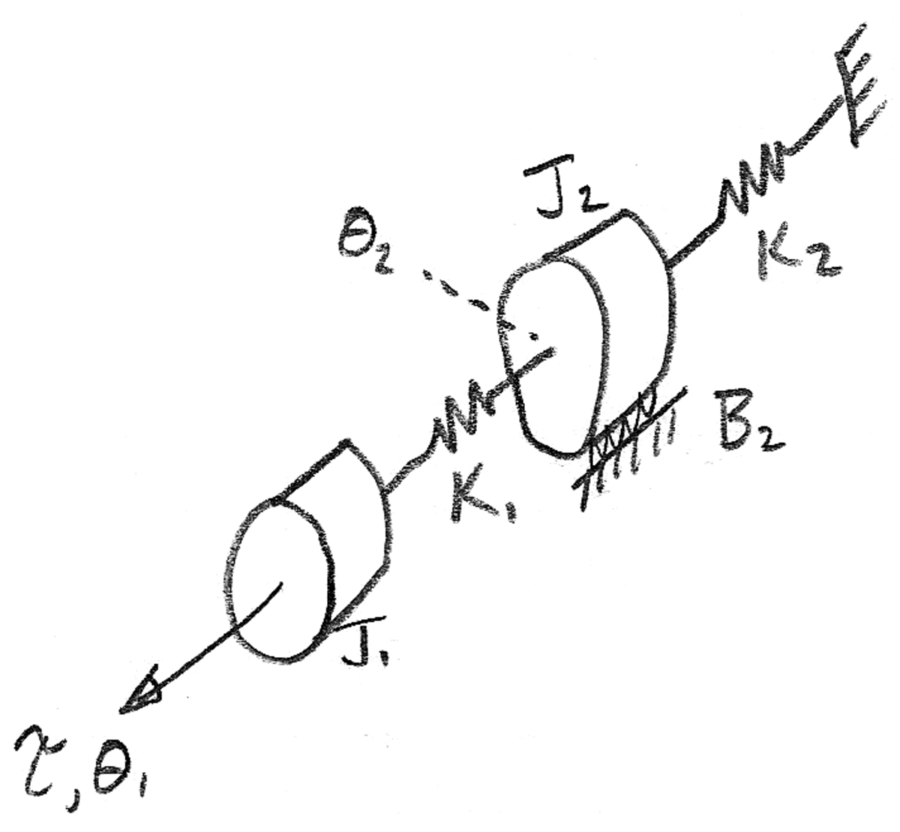
\includegraphics[width=3.0in]{figs03/00743a.png}

This system has two masses.  Although they appear to be on the same axis, they are separated by a spring and thus they can have different displacements depending on the deflection of the spring.  As a result we have two EOM:

\[
J_1\ddot{\theta_1} + K_1(\theta_1 - \theta_2) = \tau(t)
\]
\[
J_2\ddot{\theta_2} + K_1(\theta_2 - \theta_1) + K_2\theta_2 + B_2\dot{\theta_2} = 0
\]
These usually need to be solved simultaneously as with translational systems.

\end{ExampleSmall}

Once the EOMs are available, transfer functions can be derived in the same way as with translational systems.

%%%%** Section 4
\section{Gears}
%
% %%%%** Figure 2
% \begin{figure}[h]\centering
% \includegraphics[width=2.5in]{figs03/gear-spur_Emersona.jpg}
% \caption{Meshing spur gears ({\tt http://www.emersonindustrial.com/}). The large gear has 40 teeth and the small has 16.}\label{RealMeshedGears}
% \end{figure}

%%%%** Section 4.1
\subsection{Gear Kinematic Relationships}\label{gearkinematics}

A common system element in rotary systems is gears.
% (\ref{RealMeshedGears}).
The corresponding element in translational systems, levers, seem to appear less often in control systems.

Consider two meshed gears, gear 1 and gear 2 (Figure \ref{2meshedgears}).
Each gear has $N_i$ teeth.
The size of each tooth is $2\pi r_i/ N_i$.  The number of teeth which pass when a gear is rotated by $\theta_i$ is $N_i\frac{\theta_i}{2\pi}$.
Since the teeth must be the same size for the gears to mesh, we can write
\[
\frac{N_1\theta_1}{2\pi} = \frac{N_2\theta_2}{2\pi}
\]
or
\[
\frac {\theta_1}{\theta_2}  =  \frac{N_2}{N_1}
\]
differentiating we also have
\[
\frac { \dot{\theta}_1}{ \dot{\theta_2}}  =  \frac{N_2}{N_1} \qquad
\frac {\ddot{\theta}_1}{\ddot{\theta_2}}  =  \frac{N_2}{N_1}
\]

%%%%** Figure 3
\begin{figure}\centering
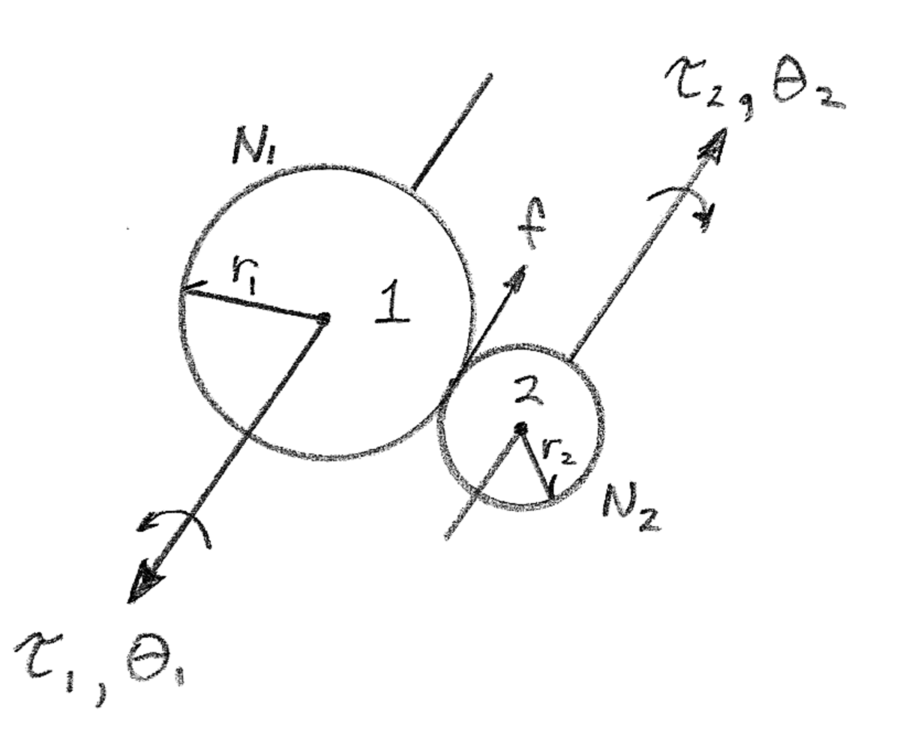
\includegraphics[width=3.0in]{figs03/00744a.png}
\caption{Two meshed gears.}\label{2meshedgears}
\end{figure}

Commonly we define $n  = N_1/N_2$.   Thus
\[
\dot{\theta_2} = n \dot{\theta_1}
\]
etc.


There is a force exerted by one tooth on the other in the tangential direction, $f$ (Figure \ref{2meshedgears}).  Since it is tangential, we can relate it easily to the torques:
\[
\tau_1 = r_1f \qquad \tau_2 = r_2f
\]
This gives
\[
\tau_1 = \frac{r_1}{r_2}\tau_2 = n\tau_2
\]
\[
\tau_2 = \frac{1}{n} \tau_1
\]

%%%%** Section 4.1
\subsection{Simplification of Geared Systems}

We can use the properties of gear transmission of rotation and torque to simplify the process of writing EOM.

Consider a damper driven by a set of gears (Figure \ref{dampergears})

%%%%** Figure 4
\begin{figure}\centering
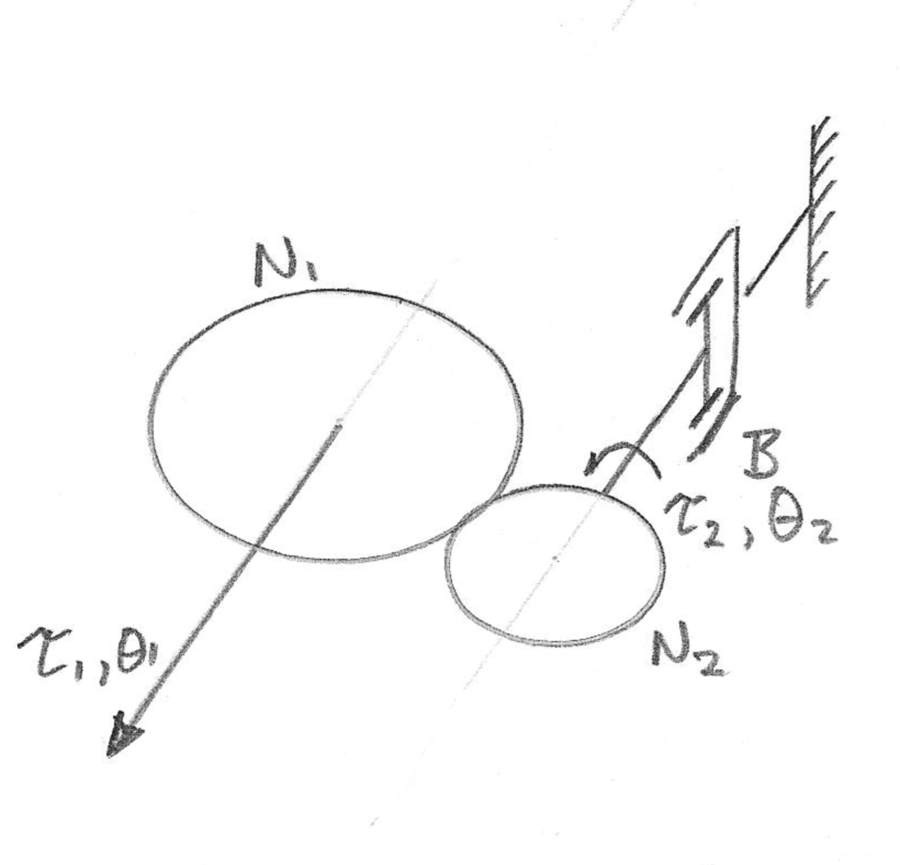
\includegraphics[width=3.0in]{figs03/00745a.png}
\caption{A viscous load (damper) driven by a set of gears.}\label{dampergears}
\end{figure}

We have
\[
\tau_2 = B \dot{\theta_2}
\]
Using the relationships above we have
\[
\frac{1}{n}\tau_1 = Bn\dot{\theta}_1
\]
or
\[
\tau_1 = Bn^2\dot{\theta}_1
\]


%%%%** Figure
\begin{figure}\centering
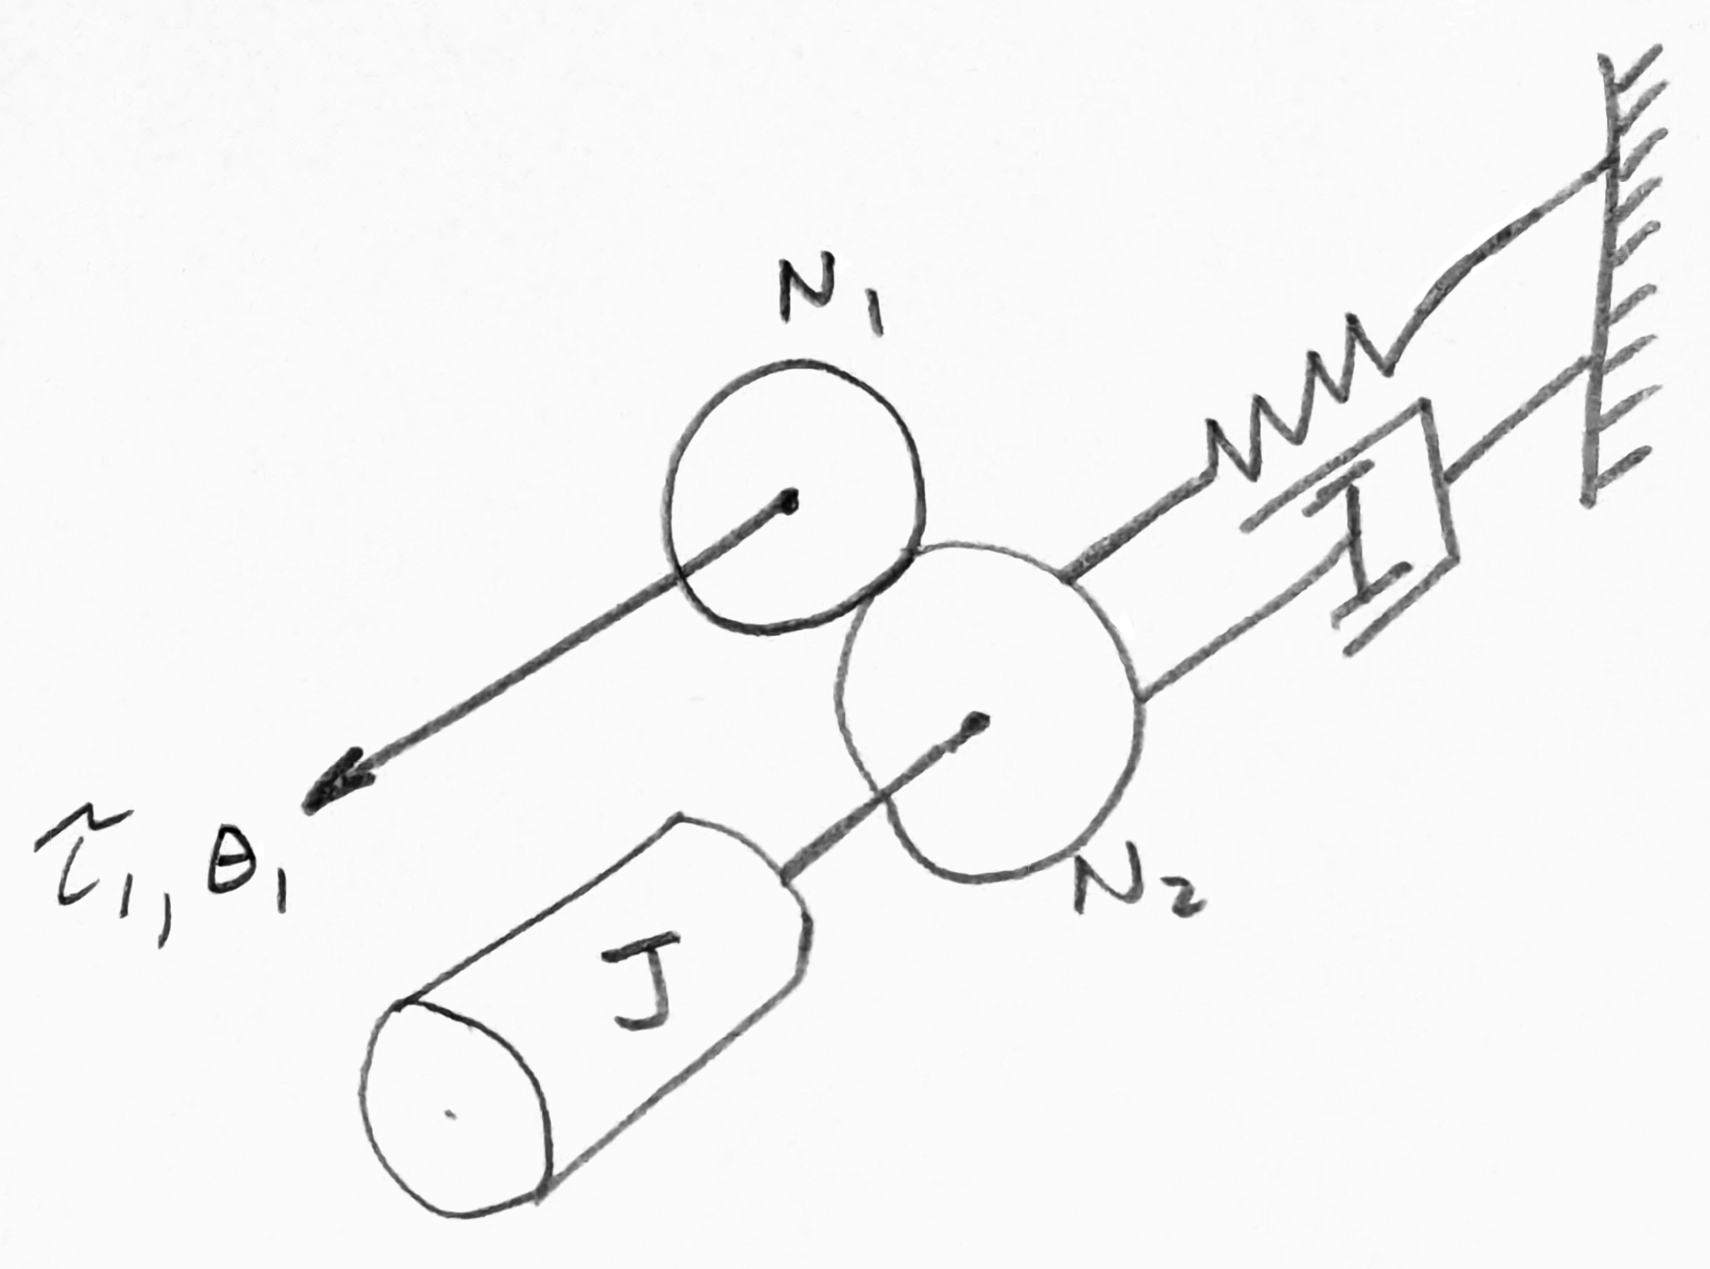
\includegraphics[width=3.0in]{figs03/J14R59.png}
\caption{A mass, spring, and damper driven by a set of gears.}\label{dampermassspringgears}
\end{figure}


Suppose the system ``beyond'' the gears had some mass and spring in addition to the damper of Figure \ref{dampergears} as shown in Figure \ref{dampermassspringgears}. The argument above would be very similar:

We have
\[
\tau_2 = J \ddot{\theta}_2 + B \dot{\theta}_2 + K \theta_2
\]
Using the relationships above we have
\[
\frac{1}{n}\tau_1 =J n \ddot{\theta}_1 + B n\dot{\theta}_1 + K n\theta_1
\]
or
\[
\tau_1 =J n^2 \ddot{\theta}_1 + B n^2\dot{\theta}_1 + K n^2\theta_1
\]

Let
\[
\hat{J} = n^2J \qquad \hat{B} = n^2B \qquad \hat{K} = n^2 K
\]
The EOM becomes
\[
\tau_1 =\hat{J}\ddot{\theta}_1 + \hat{B} \dot{\theta}_1 + \hat{K} \theta_1
\]
This is the EOM of a simpler system (Figure \ref{simplifiedgearsys}).

%%            TBD:   new modified system for this

%%%%** Figure 4
\begin{figure}\centering
  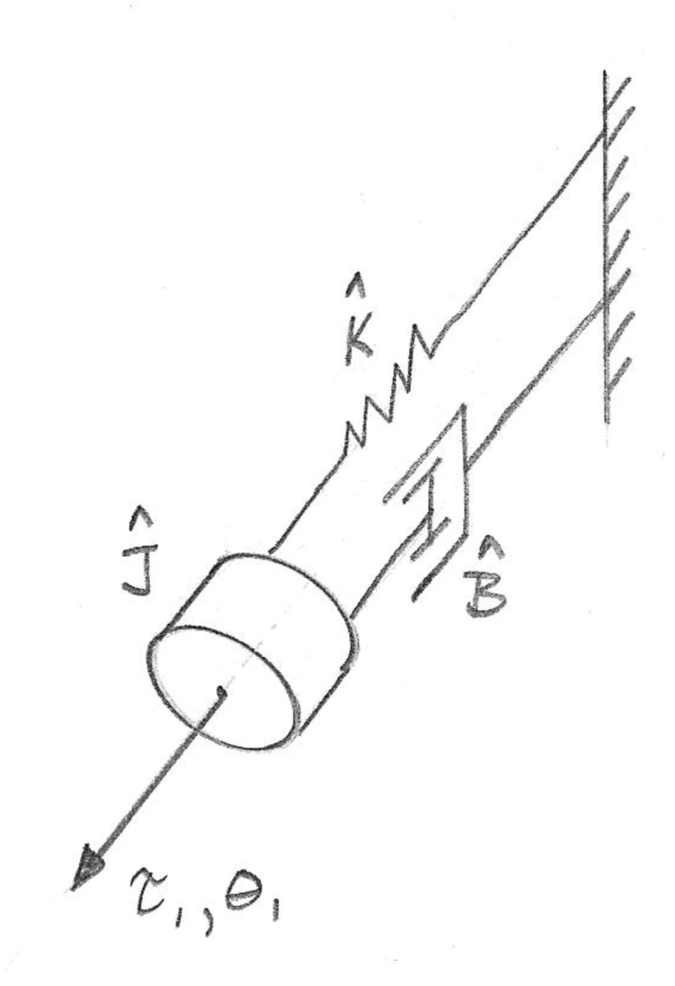
\includegraphics[width=2.25in]{figs03/00746a.png}
  \caption{Simplified equivalent system of a system modified from  Figure \ref{dampergears}}\label{simplifiedgearsys}
\end{figure}





\begin{ExampleSmall}
Transform the following geared system into an equivalent non-geared system and write the EOM.

\begin{tabular}{p{2.5in}p{2.5in}}
\vtop{\vskip-2ex \hbox{ 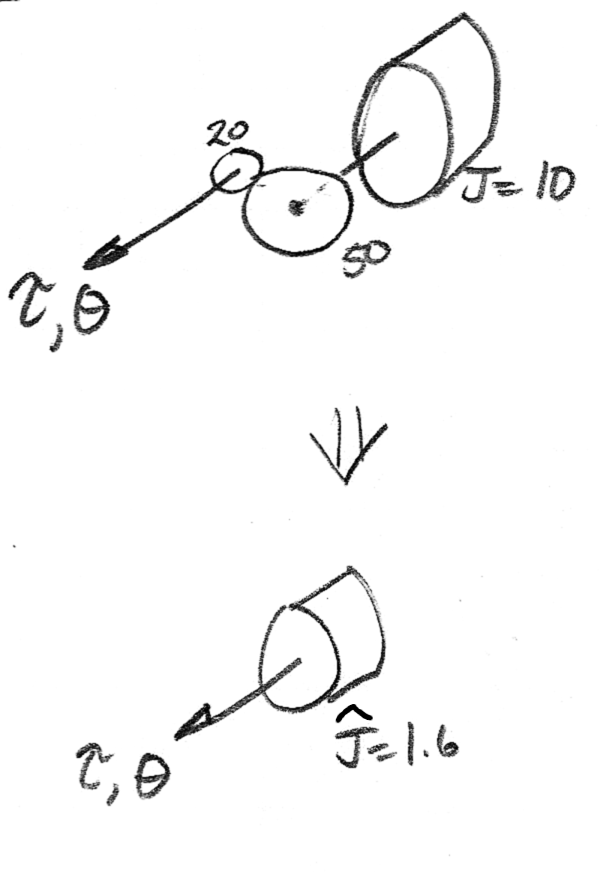
\includegraphics[width=2.0in]{figs03/00747a.png}  }}
&
\[
n = \frac {20}{50} = 0.4
\]
\[
\hat{J} = 0.4^2J = 0.16\times 10 = 1.6
\]
\[
\tau = 1.6\ddot{\theta}
\]
\end{tabular}

\end{ExampleSmall}


\begin{ExampleSmall}
Transform the following system into an equivalent system without gears

\begin{tabular}{cp{2.5in}}
\vtop{ \vskip-2ex  \hbox{  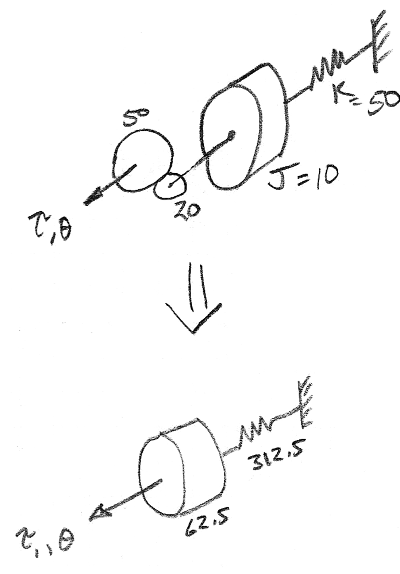
\includegraphics[width=2.0in]{figs03/00748a.png}  }}
&
\[
n = \frac {50}{20} = 2.5
\]
\[
\hat{J} = 2.5^2\times 10 = 62.5
\]
\[
\hat{K} = 2.5^2\times 50 = 312.5
\]

\[
\tau = 62.5\ddot{\theta} + 312.5\theta
\]
\end{tabular}

\end{ExampleSmall}


\begin{Example}
Transform the following system with two rotational inertias and gears to eliminate the gears, and then write and solve EOMs to get the transfer function
\[
G(s) = \frac {\theta_2(s)} {\tau(s)}
\]

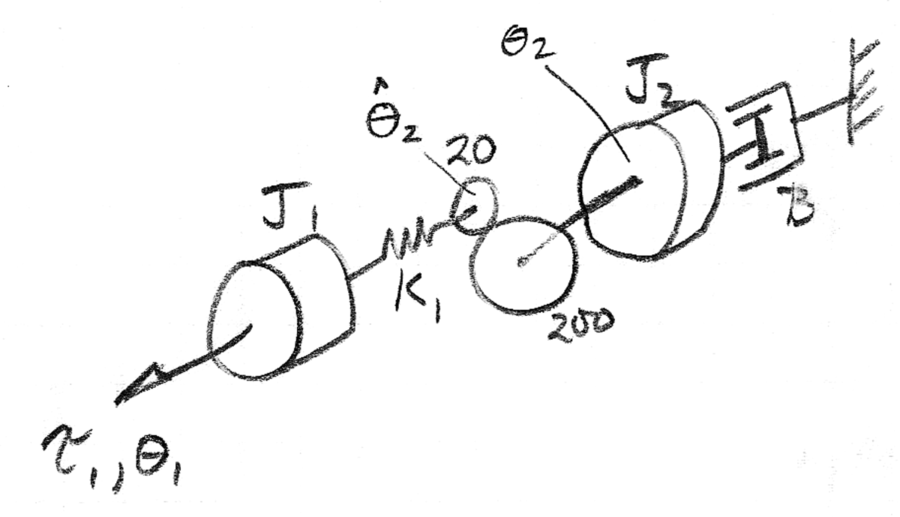
\includegraphics[width=3.0in]{figs03/00751a.png}

First, develop the transformations (by $n^2$) to change $J_2$ and $B_2$ so as to eliminate the gear set:
\[
n = \frac{20}{200} = 0.1, \quad n^2 = 0.01
\]
\[
\hat{J}_2 = 0.01 J_2 \qquad  \hat{B} = 0.01B
\]
Also, the displacement of the second inertia is changed by
\[
\hat{\theta}_2 = \frac{1}{n}\theta_2 = 10 \theta_2
\]
Note that the displacement $\theta_2$ is transformed differently from the elements $J_2,B_2$ according to the derivations in Section \ref{gearkinematics}.
Also note that $\hat{\theta}_2$ is not the same as $\theta_1$ because the spring $K_1$ can have an arbitrary deformation.

The transformed system is

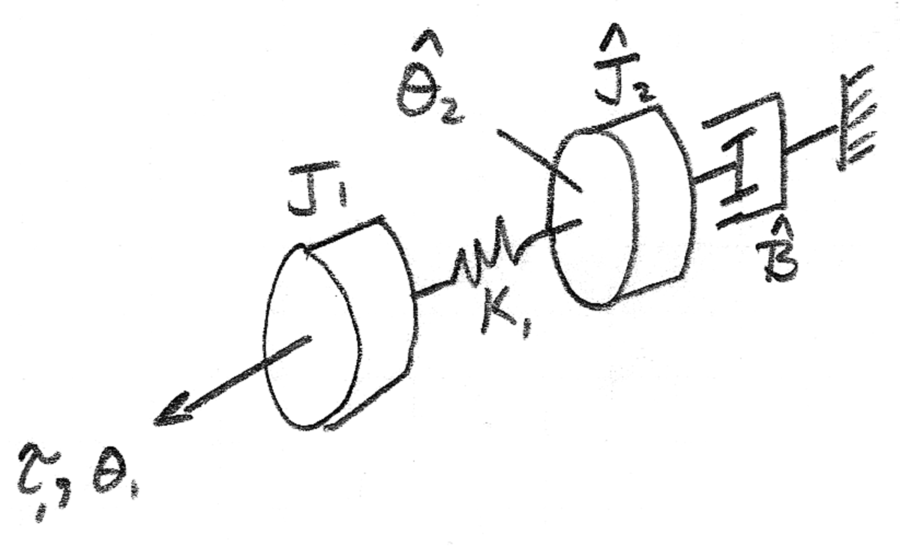
\includegraphics[width=3.0in]{figs03/00752a.png}


\end{Example}

\begin{ExampleCont}

Solving, using the techniques in Chapter 2:

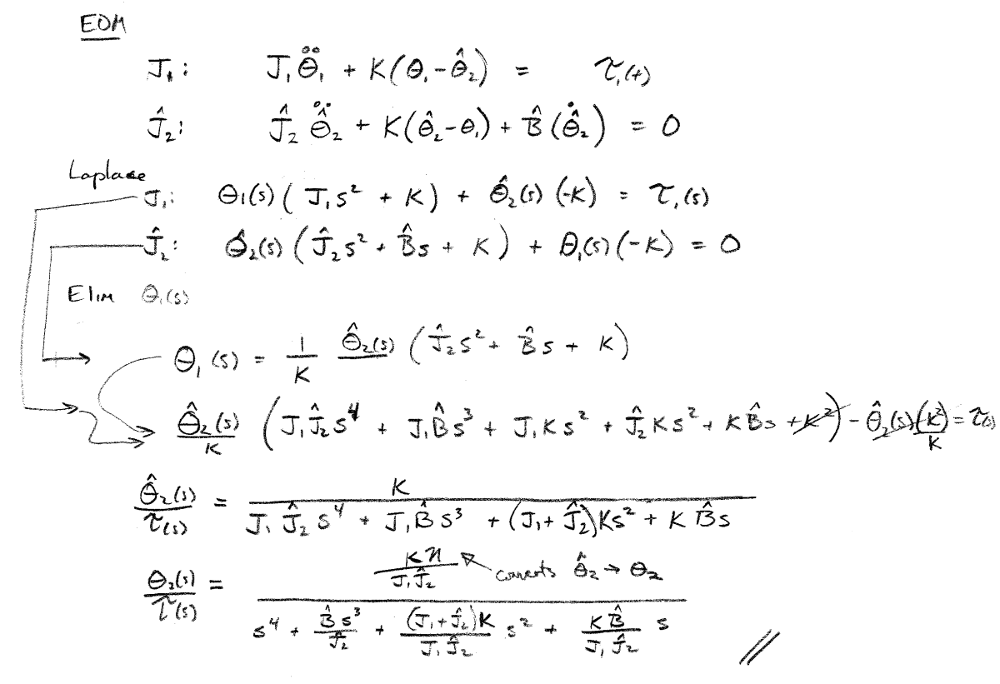
\includegraphics[width=6.0in]{figs03/00753a.png}

\end{ExampleCont}


% Problem 447 M17 P3 Sp25

\begin{Example}\label{GearTransformV1}

Consider this geared system:

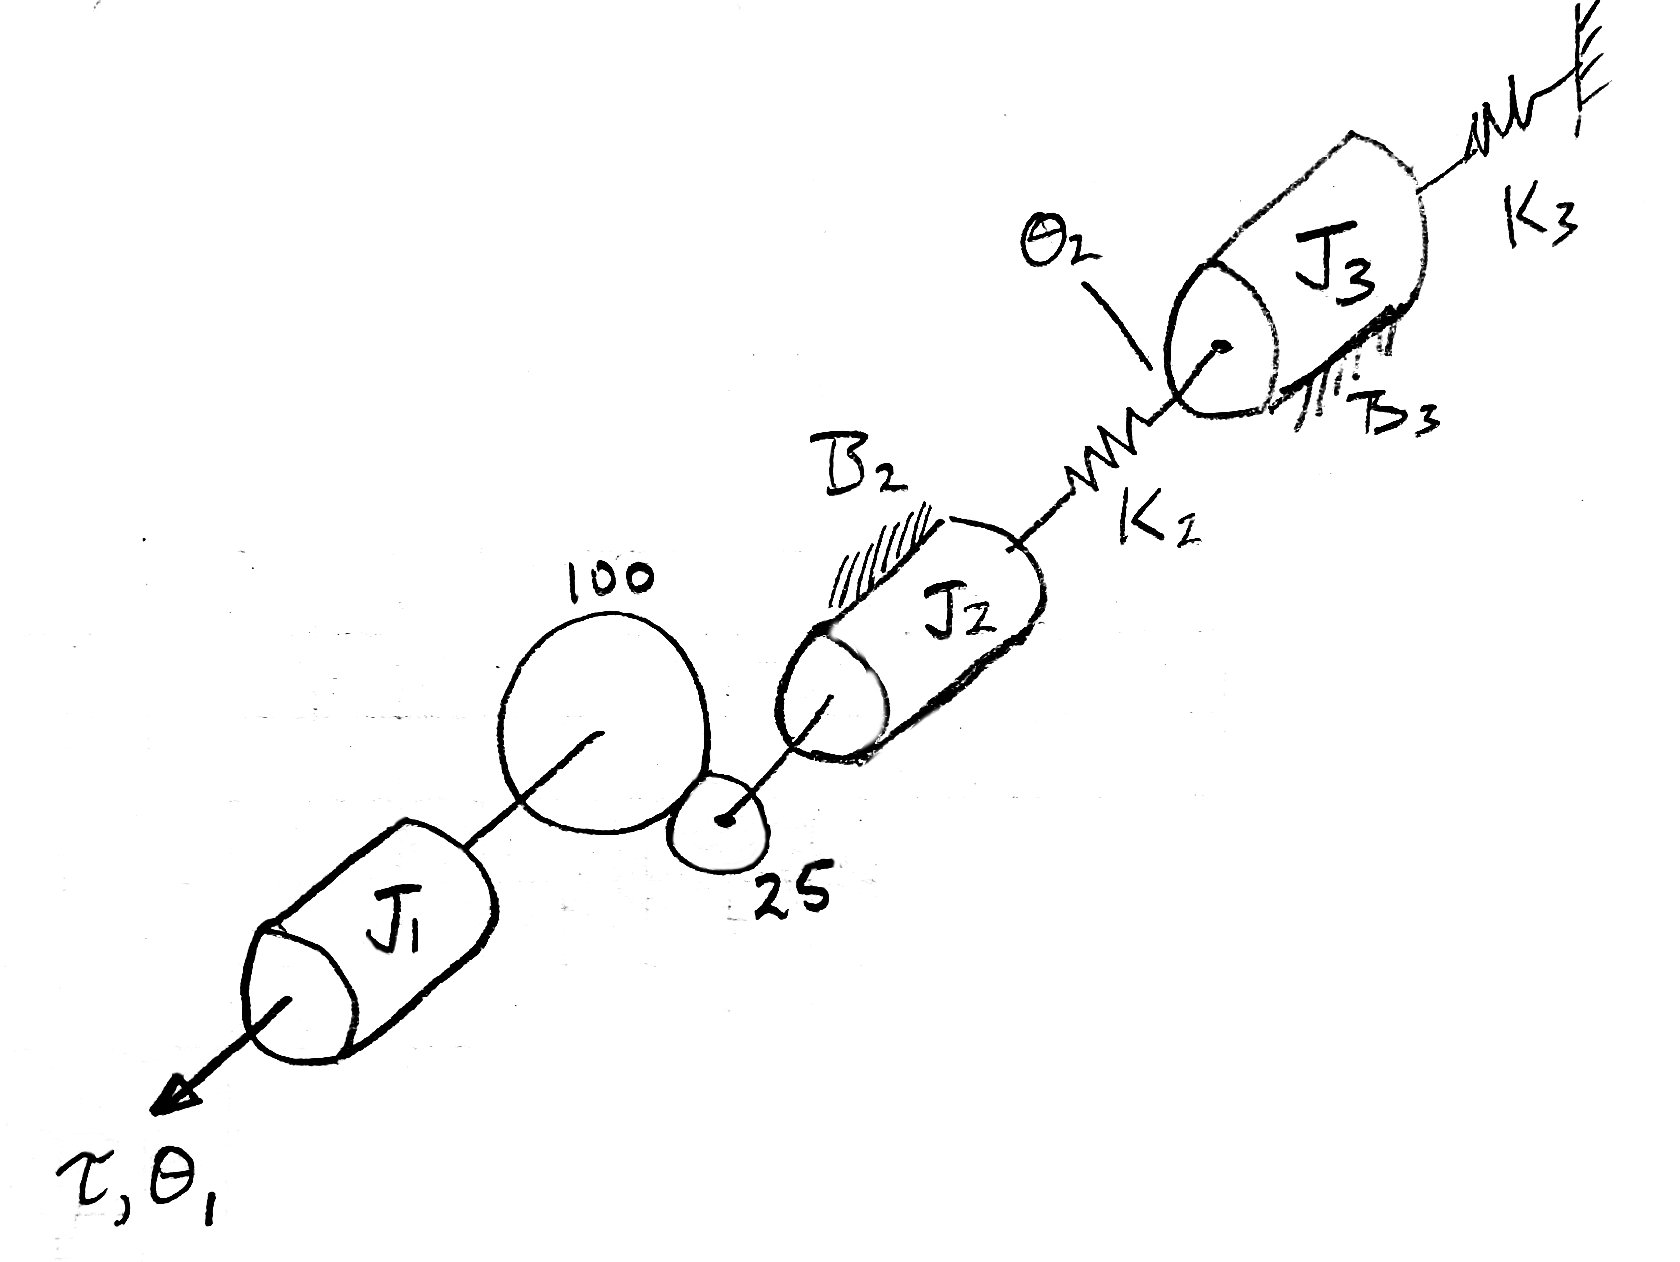
\includegraphics[width=4.0in]{figs03/R21J34.png}

We note that our gear ratio, $N= 100/25 = 4$.


\noindent
{\bf Part 1:}
Eliminate the gears and draw the transformed system:

\noindent {\bf Solution: }  Eliminating the gears and changing parameter values {\it after} the gears we get:

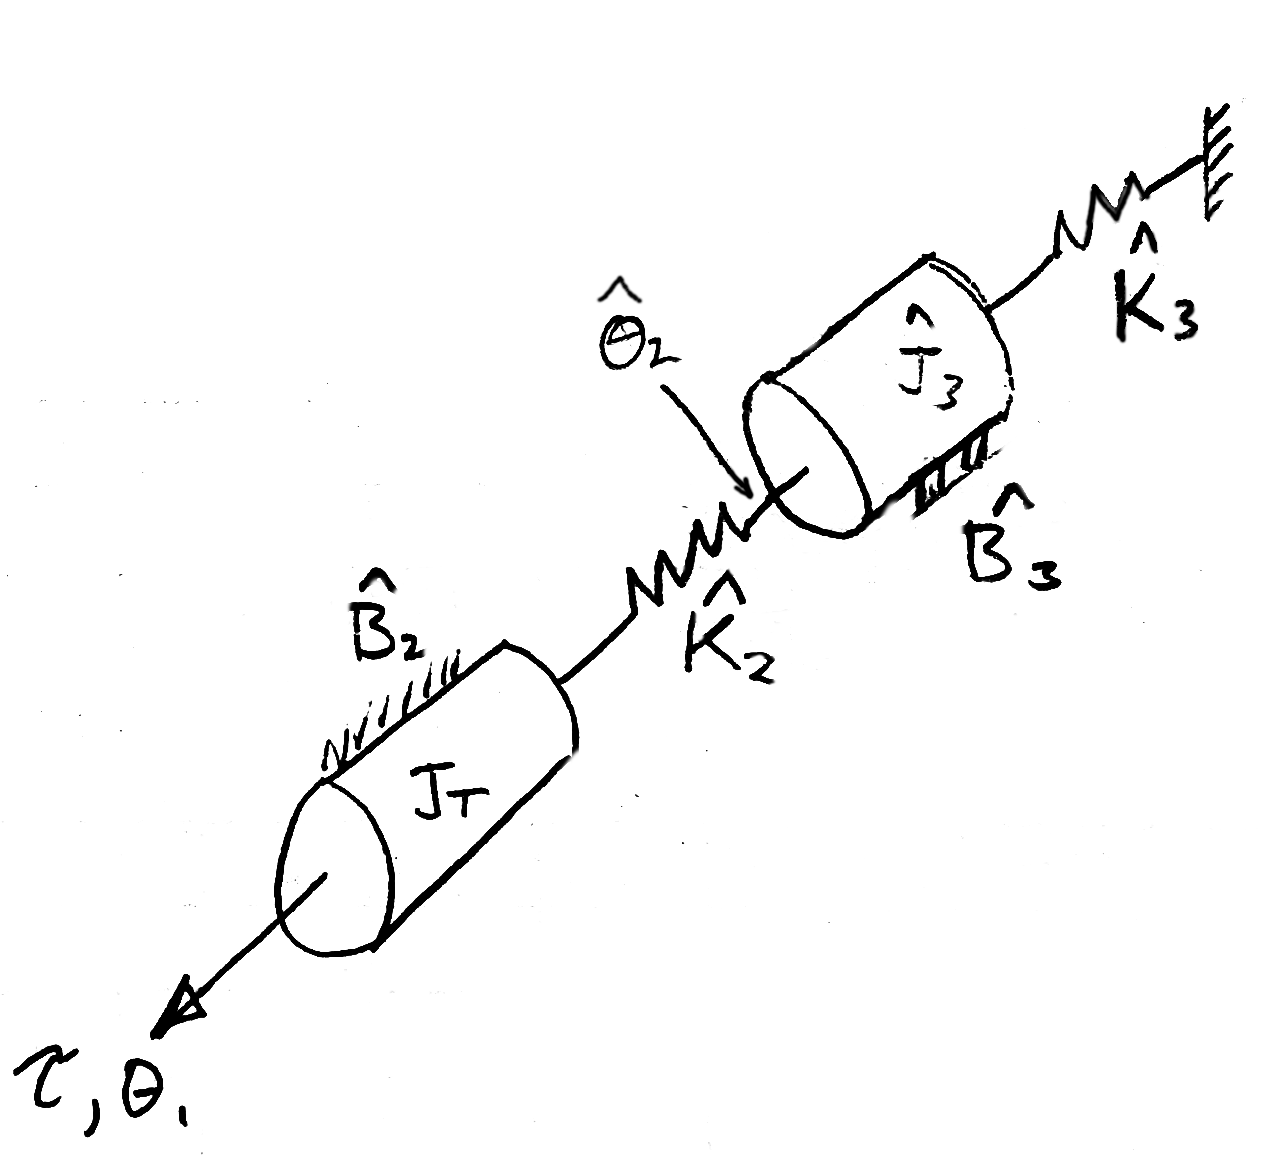
\includegraphics[width=4.0in]{figs03/R21J35.png}

where
\[
\begin{array}{rl}
N =& \frac{100}{25} = 4\\
J_T = & J_1+\hat{J}_2 = J_1+N^2J_2 \\
\hat{B}_2 =& N^2B_2\\
\hat{K}_2 =& N^2K_2\\
\hat{J}_3=&N^2J_2\\
\hat{B}_3=&N^2B_3\\
\hat{K}_3=&N^2K_3\\
\hat{\theta}_2 =& N^{-1}\theta_2 = \theta_2/4
\end{array}
\]

\end{Example}

\begin{ExampleCont}

\noindent
{\bf Part 2:}
Write the EOM(s)

\noindent {\bf Solution: }

EOM1:
\[
J_T\ddot{\theta}_1 + \hat{B}_2\dot{\theta}_1+\hat{K}_2(\theta_1-\hat{\theta}_2) = \tau
\]
EOM2:
\[
\hat{J}_3\ddot{\hat{\theta}}_2+\hat{B}_3 \dot{\hat{\theta}}_2 + \hat{K}_2(\hat{\theta_2}-{\theta}_1)+\hat{K}_3(\hat{\theta}_2)=0
\]


\noindent
{\bf Part 3:}
Substitute to eliminate all ``hats", and $N$'s in your answer
% (in other words, substitute numbers for hats and $N$ terms.)


\noindent {\bf Solution: }

EOM1:
\[
(J_1+16J_2)\ddot{\theta}_1 + 16B_2\dot{\theta}_1 + 16K_2(\theta_1-\frac{1}{4}\theta_2) = \tau
\]
EOM2:
\[
16J_3\frac{1}{4}\ddot{\theta}_2+16B_3\frac{1}{4}\dot{\theta}_2
+16K_2(\frac{1}{4}\theta_2-\theta_1) + 16K_3(\frac{1}{4}\theta_2) = 0
\]
or equivalently (for EOM2):
\[
J_3\ddot{\theta}_2 + B_3\dot{\theta}_2+K_2\theta_2-4K_2\theta_1 +K_3\theta_2= 0    % divide through by 4
\]

(a similar simplification is of course possible for EOM1.)
\end{ExampleCont}



\begin{Example}

Nick Baroody (Sp25) proposed an alternate method, which can be easier in some problems.

Consider the same system as the first diagram in Example \thechapter.\ref{GearTransformV1}.

\noindent
{\bf Part 1:}
Eliminate the gears and draw the transformed system. As an alternate transformation-based method,
leave $J_2, K_2, B_2, J_3, K_3, B_3$ as they are and transform only $J_1$ into the $\theta_2$ variables!

\noindent {\bf Solution:}
This time our gear ratio is inverted:
\[
N = 25/100 = 1/4
\]
and we have only one transform,
\[
\hat{J_1} = n^2 J_1 = \frac{1}{16} J_1
\]
We also need to transform $\tau_1, \theta_1$ according to
\[
\hat{\tau}_1 = n\tau_1 = \tau_1/4    \quad \mathrm{and} \quad  \hat{\theta}_1 = 1/n\theta_1 = 4\theta_1
\]

Our first mass is therefore
\[
J_T = J_2 + \hat{J}
\]

and the transformed system is

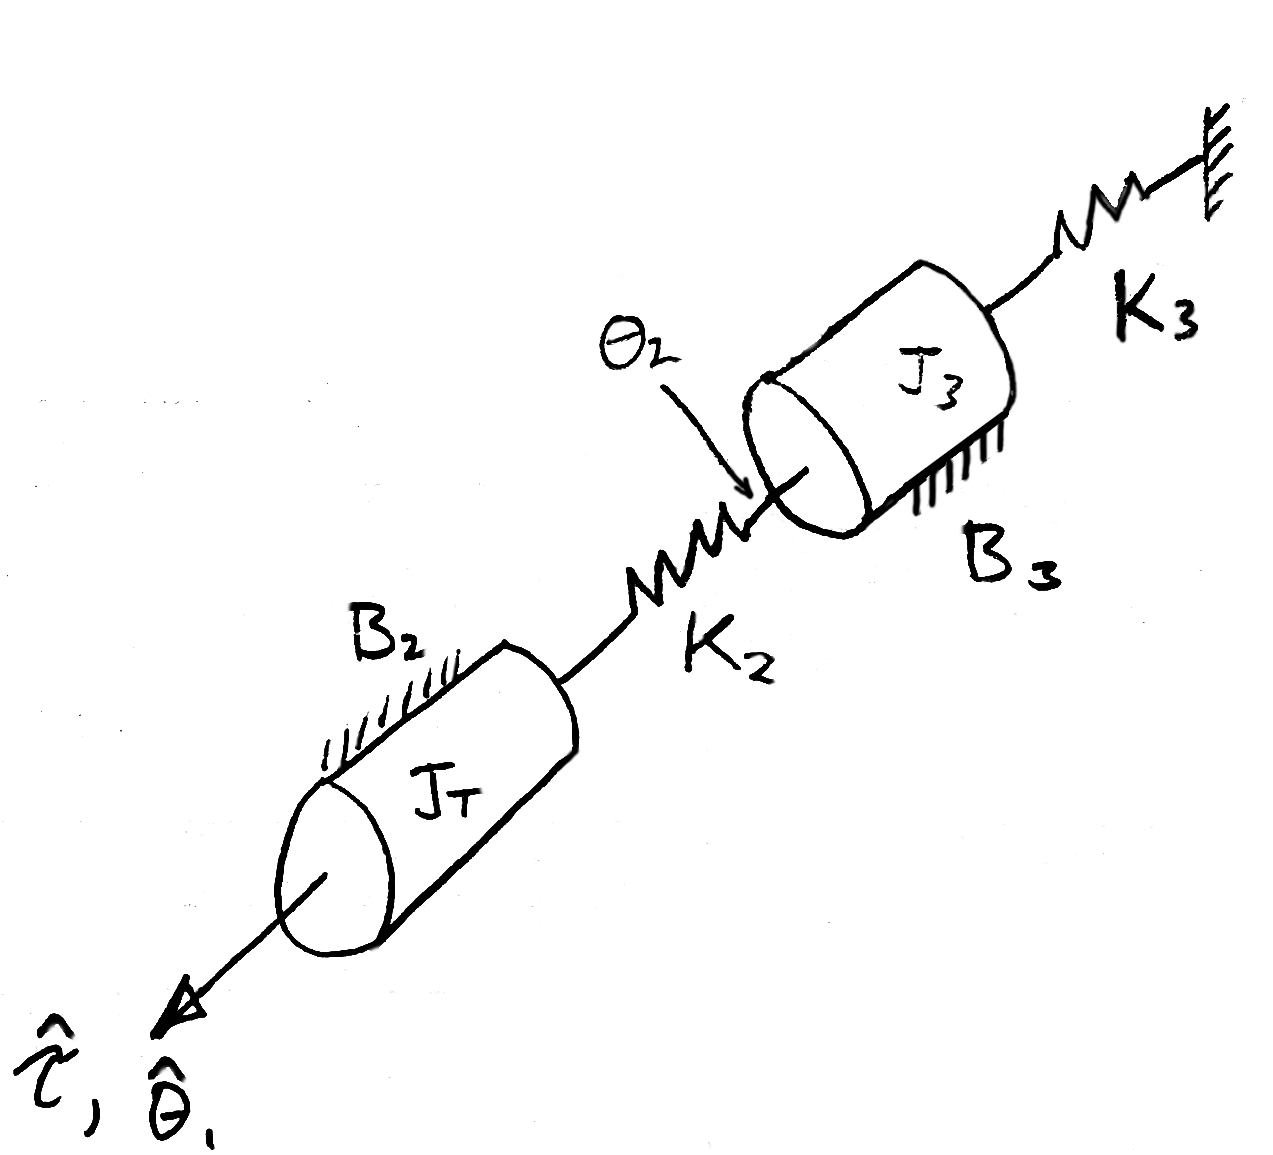
\includegraphics[width=4.0in]{figs03/R21J35rev.png}


\noindent
{\bf Part 2:}
Write the EOM(s)
\noindent Writing the  EOM's for the above figure,




\noindent {\bf Solution: }

\noindent Inertia $J_T$:
\[
J_T \ddot{\hat{\theta}}_1 + B_2 \dot{\hat{\theta}}_1 + K_2(\hat{\theta}_1 - \theta_2) = \hat{\tau}
\]

\noindent Inertia $J_3$:
\[
J_3 \ddot{\theta}_2 + B_3 \dot{\theta}_2 + K_2(\theta_2 - \hat{\theta_1}) + K_3 \theta_2 = 0
\]


\noindent
{\bf Part 3:}
Substitute to eliminate all ``hats", and $N$'s in your answer




\noindent {\bf Solution: }

\noindent $J_T$:
\[
\left(\frac{1}{16} J_1 + J_2\right)  4 \ddot{\theta}_1 + B_2  4 \dot{\theta}_1 + K_2\left(4 \theta_1 - \theta_2\right) = \frac{1}{4} \tau
\]
\[
\left(  J_1 + 16J_2\right)\ddot{\theta}_1 + 16 B_2  \dot{\theta}_1 + 16 K_2\left( \theta_1 - \frac14 \theta_2\right) =  \tau
\]
%
% \[
% \left(J_1 + 16 J_2\right) \ddot{\theta}_1 + 16 B_2 \dot{\theta}_1 + 16 K_2\left(\theta_1 - 4\theta_2\right) = \tau
% \]


\noindent $J_3$:
\[
J_3 \ddot{\theta}_2 + B_3 \dot{\theta}_2 + K_2(\theta_2 - 4\theta_1) + K_3 \theta_2 = 0
\]

Note: These are the same EOMs as the earlier method of Example \thechapter.\ref{GearTransformV1}

\end{Example}


%%%%** Section 5
\section{Rotary to Linear Motion}

% %%%%** Figure 6
% \begin{figure}\centering
% \includegraphics[width=2.5in]{figs03/stober_rack_piniona.jpg}
% \caption{Rack and Pinion drive system (Stober, {\tt www.stober.com})}\label{stoberrackpinion}
% \end{figure}

Sometimes the second gear in a chain is straightened out to $r_2 = \infty$.  The case of infinite radius corresponds to what is called a {\it rack} - a set of gear teeth arrayed in a straight line.  The gear which meshes with a rack is called a {\it pinion}.
% (Figure \ref{stoberrackpinion}).
Such systems contain a combination of rotating and translating elements and they can be analyzed by careful application of the principles developed in this and the previous chapters.

%%%%** Figure 7
\begin{figure}\centering
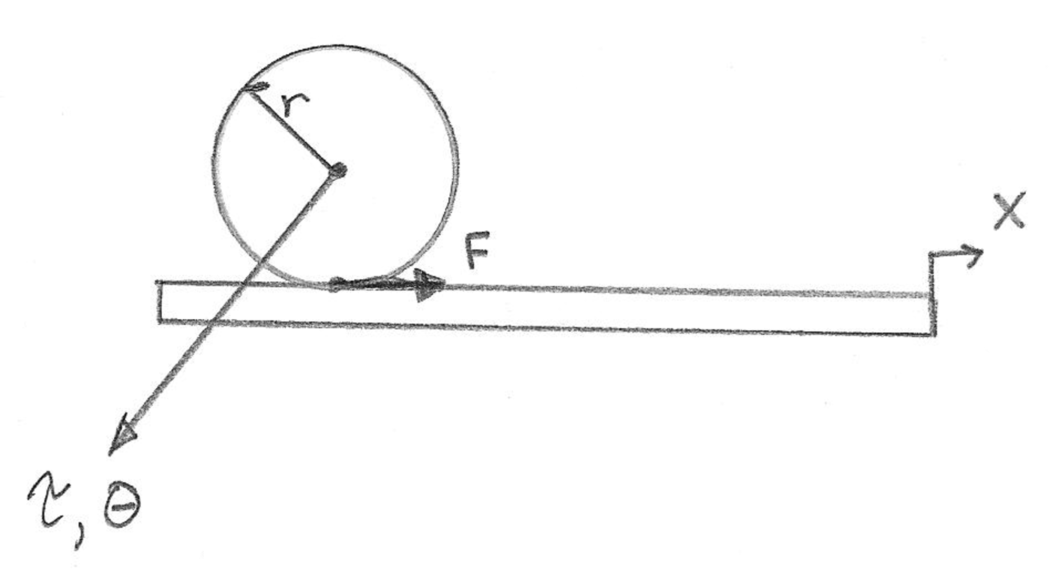
\includegraphics[width=3.5in]{figs03/00755a.png}
\caption{Rack and Pinion gear system converts rotary to linear motion and force to torque (and vice versa).}\label{basicrotarylinear}
\end{figure}


Consider the rack and pinion shown in Figure \ref{basicrotarylinear}.  Assume the gear can rotate about
its fixed axis and the rack is free to slide back and forth in the $x$ direction.
The force applied by the rack to the gear must be
\[
F = \tau/r
\]
because of the tangential contact constraint.   The displacements are related by
\[
x = r\theta
\]
by the basic geometry of circles.

In a combined system we write translational EOM(s) for the sliding components and rotational EOM(s) for the rotating components, but by substituting the relationships above, we can transform one of the EOMs so that both are in terms of rotary (or translational) variables.

When a component lies after a rotary to linear transformation, the net effect is a transformation from linear to rotary by $r^2$.   Consider the rotary-linear system shown in Figure \ref{rackpinionmasses}. Writing equations of motion:

\[
\tau = Fr + J\ddot{\theta}
\]
\[
F = M\ddot{x}
\]
Applying $x = r\theta$,
\[
F = Mr\ddot{\theta}
\]
substituting
\[
\tau = r(Mr\ddot{\theta}) + J\ddot{\theta}
\]
\[
\tau = (J+r^2M)\ddot{\theta}
\]
Note that the mass has been transformed to a rotational inertia by $r^2$.

%%%%** Figure 8
\begin{figure}\centering
\includegraphics[width=3.5in]{figs03/00822a.png}
\caption{A system containing a rack and pinion coupled to  rotary and linear masses.}\label{rackpinionmasses}
\end{figure}




%%%%%%%%%%%%%%%%%%%%%%%%%    Examples

\begin{Example}
For the system below, find  $\frac{\theta_1(s)}{\tau_1(s)}$

\includegraphics[width=3.5in]{figs03/00754a.png}

The initial EOMS are
\[
J_1\ddot{\theta}_1 + rF = \tau_1
\]
\[
M_1\ddot{x}_1 + K(x_1-x_2) = F
\]
\[
M_2\ddot{x}_2+K(x_2-x_1)  = 0
\]

\includegraphics[width=6.0in]{figs03/00756aa.png}
%
% \end{Example}
%
% \begin{ExampleCont}

\includegraphics[width=6.0in]{figs03/00756ba.png}

Note that the system has no dampers and also it has two poles at $s=0$.

\end{Example}

% \end{ExampleCont}

   % Rotational Dynamics
% 

\chapter{Basics of State Space}\label{BasicsStateSpaceChapter}


\section{Problem Statement and Learning Objectives}

Most of this course will cover control system design using system transfer functions (rational polynomials in $s$ which describe the input-output relationships of system blocks).  However when we write the equations of motion, it is an ideal time to introduce a couple of concepts from the ``modern control theory'' introduced in the 1960's which has supplanted the $s$ domain methods in some applications.

\paragraph{Learning Objectives}
Be able to
\begin{itemize}
    \item Understand the basic system equations to represent a linear
    dynamic system in state space.
    \item Convert equations of motion (EOMs) into state space
    representation.
    \item Use the computer to plot step response and state trajectories from
    the state space model.
\end{itemize}

\section{Introduction}
In ``modern'' control theory, the system is represented as a first order linear differential equation in a high dimensional space known as state space.  Each point in state space represents a unique dynamical state of the system.   For example, a system with one mass could be described by a 2-dimensional state space consisting of the position, $x$ and the velocity, $\dot{x}$ (Figure \ref{2Dstatespace}).

\begin{figure}\centering
\includegraphics[width=65mm]{figs04/01069.png}   \hspace{0.25in}
\includegraphics[width=45mm]{figs04/01075.png}
\caption{Translational dynamic system for state space example.}\label{2Dstatespace}
\end{figure}

One way to define the dimensionality of a system's state space is to identify all system variables which describe an energy.  Each one is a dimension of state space.   In our single mass example, energy is stored in the spring and mass:
\[
E_K = \frac{1}{2}(K_1 + K_2)x^2 \qquad E_M = \frac{1}{2}M{\dot{x}}^2
\]
So for this system we would use $x$ and $\dot{x}$ as state variables.
We use a vector, $X$, to define a point in state space such as:
\[
X = \begin{bmatrix} x \\ \dot{x} \end{bmatrix}
\]
Then the dynamics of the system are represented in a matrix first order LODE:
\[
\dot{X} = AX+BU
\]
Where $X$ is the state vector, $\dot{X}$ is the first derivative of the state vector,
\[
\dot{X} = \begin{bmatrix}\dot{x} \\ \ddot{x} \end{bmatrix}
\]
$A$ is a matrix of constant coefficients,
$U$ is the system input (like an applied force, $f(t)$), and
$B$ is another matrix.  This form can represent systems with multiple inputs (the elements of $U$), but here we will restrict ourselves to a single input so only one element of $U$ is non-zero.

Sometimes the output of the system, $Y$, is not one of the state variables, but instead a linear
combination of the state variables and possibly the input.  In this case there is another equation
\[
Y = CX+DU
\]
where $C,D$ are additional matrices of constant coefficients.
There is no Laplace transform and the
equations come directly from the equations of motion. In many realistic systems,
many  elements of these matrices are zero.



\section{System Matrices from Equations of Motion}\label{SecSystemMatricesFromEOMs}
Let's see how EOMs turn into the State Space representation using the example system of Figure \ref{2Dstatespace}.  Writing the EOM:
\[
M\ddot{x}+B\dot{x}+(K_1+K_2)x = f(t)
\]
rearranging to solve for $\ddot{x}$:
\[
\ddot{x} = \frac{1}{M}\left[ -B\dot{x}-(K_1+K_2)x+f(t)\right ]
\]
\[
\ddot{x} = -\frac{B}{M}\dot{x} - \frac{K_1+K_2}{M}x + \frac{1}{M}f(t)
\]
Converting this to a matrix equation is just rearranging according to
\[
       \dot{X} = \begin{bmatrix}\dot{x} \\ \ddot{x} \end{bmatrix}
\qquad      X  = \begin{bmatrix} x \\ \dot{x} \end{bmatrix}
\qquad U       = \begin{bmatrix}0\\f(t)\end{bmatrix}
\]
%  \begin{bmatrix}\end{bmatrix}
then we have
\[
\dot{X} =
\begin{bmatrix}\dot{x} \\ \ddot{x} \end{bmatrix} =
\begin{bmatrix}0&1\\\frac{-(K_1+K_2)}{M}&\frac{-B}{M}\end{bmatrix}
\begin{bmatrix}x\\ \dot{x}\end{bmatrix}+
\begin{bmatrix}0&0\\0&\frac{1}{M}\end{bmatrix}
\begin{bmatrix}0\\f(t)\end{bmatrix}
\]
The top row is sort of a trivial equation, and the second row is the rearranged equation of motion.
This is the state space description for the system of Figure \ref{2Dstatespace}.


\begin{Example}\label{suspensionstatespace}
Consider the car suspension
Example 2.\ref{ExampleCarSuspension} and Example 2.\ref{ExampleCarSuspensionTF}.
\vspace{0.2in}
Derive the state space representation.

The EOMs were:
\begin{align*}
&M_w\ddot{x}_2+B_s(\dot{x}_2-\dot{x}_3)+K_s(x_2-x_3)+K_t(x_2-x_1) =0 \\
&M_v\ddot{x}_3+B_s(\dot{x}_3-\dot{x}_2)+K_s(x_3-x_2) = 0
\end{align*}
Note that the input to this system is $x_1$, the displacement of the road.  We  can
re-write the EOMS to put the input on the RHS:
\begin{align*}
&M_w\ddot{x}_2+B_s(\dot{x}_2-\dot{x}_3)+K_s(x_2-x_3)+K_tx_2 = K_tx_1 \\
&M_v\ddot{x}_3+B_s(\dot{x}_3-\dot{x}_2)+K_s(x_3-x_2) = 0
\end{align*}
Let the state vector be:
\[
X = \begin{bmatrix}x_2 & \dot{x}_2 & x_3 & \dot{x}_3\end{bmatrix}^T
\]
(where T indicates transpose to make $X$ a column vector)
and its derivative is
\[
\dot{X} = \begin{bmatrix}\dot{x}_2 & \ddot{x}_2 & \dot{x}_3 & \ddot{x}_3\end{bmatrix}^T
\]
Rearranging the EOMS:

\begin{align*}
\ddot{x}_2  &= \frac{1}{M_w}\left [-(K_T+K_s)x_2-B_s\dot{x}_2+K_sx_3+B_s\dot{x}_3\right]\quad+\quad \frac{1}{M_w}K_tx_1 \\
\ddot{x}_3 &= \frac{1}{M_v}\left[+K_sx_2+B_s\dot{x}_2 -K_sx_3-B_s\dot{x}_3\right]
\end{align*}

We then have the 4x4 matrix state equations:
\[
\dot{X} = \begin{bmatrix}\dot{x}_2 \\ \ddot{x}_2 \\ \dot{x}_3 \\ \ddot{x}_3\end{bmatrix}
=
\begin{bmatrix} 0&1&0&0\\
-\frac{(K_T+K_s)}{M_w}&\frac{-B_s}{M_w}&\frac{K_s}{M_w}&\frac{B_s}{M_w}\\
0&0&0&1 \\
\frac{K_s}{M_v}&\frac{B_s}{M_v}&\frac{-K_s}{M_v}&\frac{-B_s}{M_v}\\
\end{bmatrix}
\begin{bmatrix}x_2\\\dot{x}_2\\x_3\\\dot{x}_3 \end{bmatrix}+
\begin{bmatrix}
    0&0&0&0&\\
    0&\frac{K_t}{M_w}&0&0&\\
    0&0&0&0&\\
    0&0&0&0&\\
\end{bmatrix}
\begin{bmatrix} 0 \\x_1\\0\\ 0\end{bmatrix}
\]
Note that we have two trivial equations: rows 1 and 3:
\[
\dot{x}_2 = \dot{x}_2 \qquad \dot{x}_3 = \dot{x}_3
\]
Once your parameter values are known, you can plug them in and it is easy to evaluate the response to any input using the computer.
\end{Example}

%
% To see that there are infinitely many SS representations of a linear system, consider a
% rotation matrix such as
% \[
% R = \begin{bmatrix}1 & \cos{\theta} \\ -\sin{\theta} & 1\end{bmatrix}
% \]
% (such a matrix is called ``orthonormal'' and has eigenvalues of unit magnitude).   The key point
% is that multiplying a matrix by a rotation matrix does not change its eigenvalues at all.   Therefore,
% if $R$ is orthonormal we can write
% \[
% RY = RAX+RBU
% \]
% and we have a new system matrix  $RA$ which represents the same system as $A$.
%


\subsection{Sources}
For Toyota Camry Suspension Parameters:
\begin{itemize}
    \item R.K. Taylor, L.L. Bashford, M.D. Schrock, ``Methods for Measuring Vertical Tire Stiffness,''
    Transactions of ASAE, vol 34, p 1415-1419, 2000
    \item M.D. Rao, S.Gruenberg, ``Measurement of Equivalent Stiffness and Damping of Shock Absorbers,''
    \item J. Iwaniec, ``Identification Of Car Suspension System Parameters On The Basis Of Exploitational Measurements,'' Diagnostyka, V14, N2, 2013
\end{itemize}

     % State Space Intro
% %
%
%

\chapter{Transient Response and Frequency Response}\label{2ndOrderTransientChapter}

This chapter starts with fairly detailed analaysis of second order linear systems and the concepts of magnitude and frequency of steady state sinusoidal response.  Computer techniques easily create highly accurate frequency response plots.   We then develop   techniques for hand drawing reasonably accurate frequency responses.   While the hand techniques initially seem rather involved, after performing a few practice problems (and checking the results on the computer) they can be executed very rapidly with low effort.

\section{Problem Statement and Learning Objectives}
Be able to
\begin{itemize}
    \item Use the partial fraction expansing and basic Laplace Transform pairs to
    solve the step response of a 2nd order system.
    \item Explain how the location of poles of a 2nd order system in the $s$-plane
    affects the envelope and oscillation frequency of the step response.
    \item Explain the meaning of ``steady state sinusoidal response".
    \item Evaluate the steady state sinusoidal response magnitude of a transfer function
    at a specified frequency $\omega$.
    \item Evaluate the steady state sinusoidal response phase of a transfer function
    at a specified frequency $\omega$.
    \item Express a positive quantity in decibels (dB) and rapidly perform basic manipulation of
    logarithmic quantities.
    \item Use dB to rapidly compute  the steady state sinusoidal response magnitude of a transfer function
    at a specified frequency $\omega$.

    \item Hand sketch a Bode asymptotic magnitude plot with ``$\pm3dB$" corrections.
    \item Hand sketch a Bode asymptotic phase plot with smooth approximations,
    and explain relationships between the Bode magnitude and phase plots.
    \item Make detailed corrections to asymptotic Bode plots for systems containing complex conjugate poles and zeros.

\end{itemize}


\section{Introduction}
This chapter will introduce calculation of the response of systems which we have described
by transfer functions.   First we consider step response of a 2nd order system in the time
domain.   Step response of higher order systems requires numerical evaluation but we can
build much intuition from considering 2nd order systems.   Secondly,  we will study steady
state output corresponding to constant sinusoidal inputs and develop methods to
hand-sketch magnitude and phase of the output response for a system of any order.

Although it is easier to do both of these computations with the computer, basic hand skills
are studied because they develop better intuition and understanding of systems and system response
results.  The basic analytical approach is to understand the big picture by hand sketching
these responses first, to a practical level of accuracy, and then easily
create very accurate plots with the computer for detailed analysis.

\section{The basic 2nd order dynamical system}

A dynamical system is said to be ``second order" if the highest power of $s$ in its denominator  is 2.  An example of such a system is

\[
G(s) = \frac1{(s-a)(s-b)} = \frac {1}{s^2 -(a+b)s+ab}
\]


$a$ and $b$ are roots of the polynomial in the denominator.  When $s$ equals a root, the denominator = 0 and
\[
G(a) = G(b) = \infty
\]

Because $G(s)$ goes up to infinity at these locations, $a,b$,  in the complex plane, we call $a$ and $b$ ``poles" of the transfer function
$G(s)$.

\newpage

\begin{ExampleSmall}

Find the poles of the transfer function
and use the partial fraction expansion and the computer to evaluate the step response output, $Y(s)$.
\[
G(s) = \frac{Y(s)}{X(s)} = \frac {1}{(s^2 + 13s + 30)}
\]
By either simple factoring or use of the quadratic formula,
\[
G(s) = \frac{1}{(s+3)(s+10)}
\]
Thus the poles of G(s) are $s=\{-3,-10\}$.   To add a step input to the system, we multiply by
\[
U(s) = 1/s
\]
giving the output $Y(s)$:
\[
Y(s) = U(s)G(s) =  \frac{1}{s(s+3)(s+10)}
\]


The partial fraction expansion is
\[
G(s) = A_1/s + A_2 /  (s+3) + A_3/ (s+10)
\]
Solving for $A_1,A_2, A_3$,
\[
A_1 = 1/30   \qquad A_2 = -1/21 \qquad A_3 = 1/70
\]
Applying the inverse transforms for $\frac{1}{s}$ and $\frac{A}{(s+a)}$,
\[
g(t) = 0.0333u(t) - 0.0476 e^{-3t} + 0.0143e^{-10t}
\]
Plotting the function $g(t)$ by computer (Left):

\begin{tabular}{cc}
\includegraphics[width=3.0in]{figs05/realstepa.png}
&
\includegraphics[width=3.0in]{figs05/step_components.png}
\end{tabular}

Note that g(t) has three components,  $0.0333u(t)$, $ - 0.0476 e^{-3t}$, $ +0.0143e^{-10t}$.   Plotting
them separately (Right), we see how they combine to create the response


\end{ExampleSmall}


\begin{ExampleSmall}
Find the poles of the transfer function,
\[
G(s) = \frac{400}{12.7s^2 + 304.8s + 2641.6}
\]
and plot the step response by computer.

\vspace{0.25in}
Applying the quadratic formula to get the roots of the denominator:

\[
\{a,b\} = \frac {-304.8 \pm \sqrt{304.8^2 -4\times12.7\times2641.6}}{2\times 12.7}
\]
\[
\{a,b\} = \{(-12+j8),(-12-j8)\}
\]
In this case the poles are complex numbers.

Note that these numbers were kind of messy. This illustrates a good reason to normalize the denominator polynomial.   Lets do the problem again but with a normalized denominator:

\[
G(s) = \frac{3.15}{s^2 + 24s + 208}
\]
Applying the quadratic formula to get the roots of the denominator:

\[
\{a,b\} = \frac {24 \pm \sqrt{24^2 -4\times208}}{2}
\]
This is simplified because the $s^2$ coefficient (`$a$' in the quadratic formula) is one.  The result is the same.
\[
\{a,b\} = \{(-12+j8),(-12-j8)\}
\]

Plotting the step response by computer:

\includegraphics[width=3.5in]{figs05/cplxstepa.png}
\end{ExampleSmall}


There are lots of ways we could express the simple polynomial in the denominator of $G(s)$ and we'll play around with a few:

\[
G(s) = \frac{1}{s^2+us+v} \qquad (u = -(a+b),\quad v= ab)
\]
Now let's introduce a parameter $\omega_n$ (pronounced ``omega-n"):
\[
\omega_n  = \sqrt{v} = \sqrt{ab}
\]
and another one, $\zeta$ (``zeta"):
\[
\zeta = \frac{u}{2\sqrt{v}} = \frac{-(a+b)}{2\sqrt{ab}}
\]

if we make these substitions, our transfer function becomes
\[
G(s) = \frac{1}{s^2 + 2\zeta\omega_n s+\omega_n^2}
\]

So far this is just playing around with notation.  The point  however is that $\zeta$ and $\omega_n$, called the {\it damping ratio} and {\it natural frequency} respectively, give important insights not obvious from the poles ($a,b$) themselves.

If the poles are complex, we know that they must  be complex conjugates of each other. In other words,
\[
Re(a) = Re(b) \qquad Im(a) = -Im(b)
\]

Using the properties of complex numbers, and the fact above, it is simple to show

\[
\omega_n = \sqrt{Re(a)^2 + Im(a)^2} = |a| = |b|
\]
\[
\zeta = -Re(a)/\omega_n = \cos\left(\arctan\left(\frac{Im(a)}{-Re(a)}\right)\right)
\]

If we plot these points on the complex plane (Figure \ref{ccpoleszeta}) we can see why these parameters give a different view from the poles:
they represent the poles $e.g. p$ in polar coordinates.

\[ \angle p = \cos^{-1}(\zeta) \quad |p| = \omega_n
\]


\begin{figure}\centering
 \includegraphics[width=4.25in]{figs05/00733a.png}
\caption{Complex conjugate poles in the complex plane can be represented in Cartesian Coordinates ($r+jm$) or polar coordinates $\{\zeta, \omega_n\}$}\label{ccpoleszeta}
\end{figure}

\subsection{Pole Location and Step Response}

The location of poles in the complex plane determines the characteristics of the dynamic response to system inputs.  One input which we care about a lot is the step function

\[
u(t) = \left \{ \begin{array}{cc} 0 & t< 0 \\ 1 & t >= 0 \end{array} \right .
\]

The Laplace transform of the step input is $U(s) = \frac{1}{s}$.

The response to  a step input determines what the system will do when we ``change our minds" about what the output should be.  For example, you walk into a room and turn the thermostat from $50^\circ$ to $68^\circ$ or you press ``Resume" on your cruise control.


When we take a 2nd order transfer function of the form $G(s) = \frac{M}{(s+a)(s+b)}$, and multiply it by the step input, we get the output
\[
Y(s) = \frac{1}{s}\frac{M}{(s+a)(s+b)},
\]
we can expand it using the partial fraction expansion (Section \ref{partialfractionsection}) into the form
\[
Y(s) = \frac{A_0}{s} + \frac{A_1}{(s+a)}+  \frac{A_2}{(s+b)},
\]

and further,  the inverse transform of each term in the partial fraction expansion is

\bq\label{dampedexponentialsolution}
y(t) = A_0 +  A_1e^{at} + A_2e^{bt}   \qquad (t>= 0)
\eq

It can be shown that for a 2nd order system with a pair of complex conjugate poles, $\{a,b\}$, this solution takes the form

\bq\label{eqnDampedSinStep}
y(t) = A_0-|A_1|e^{-\zeta\omega_n t} (\cos({\omega_dt +\phi}))
\eq

In this response, the exponential term {\it multiplies } the sinusoid term.  Since the sinusoid cannot exceed the range $-1<=sin(\omega t)<=1$, the response will be bounded by the exponential and we will call it the ``envelope" since it ``contains" the sinusoidal part of the response.
Let's look at some examples of this function.  For $\omega_n = 0.4$, and $\zeta=.124$ (corresponding to the poles: $s = -0.05\pm0.4j$), we get the step response shown in Figure \ref{typicalstep}



\begin{figure}\centering
\includegraphics[width=3.5in]{figs05/typical_stepa.png}
\caption{Step response of a typical system ($\omega_n = 0.4, \zeta=.124$ ) with complex conjugate 2nd order poles. The envelopes (red and green) are also shown.}\label{typicalstep}
\end{figure}



Now, let's place these responses according to the location of their complex poles.  Figure \ref{splaneresponse} represents the top half of the complex plane.   Each plot is the response of a 2nd order system having one of its complex conjugate poles in its rough location.  Note that the last two columns have positive real parts to their poles.



\begin{figure}\centering
  \includegraphics[width=6.5in]{figs05/s_plane_responsesa.png}
  \caption{Step responses of 2nd order systems with the pole locations labeled above each plot. The array of sub-plots represents part of the upper half of the complex plane.}\label{splaneresponse}
\end{figure}


Looking at Figure \ref{splaneresponse} there are two key patterns.  First, the frequency of the sinusoid increases as the imaginary part of the pole increases.  Second the envelope grows with time when the real part is positive, and shrinks over time when the real part is negative.   The larger the magnitude of the real part, the faster the envelope changes.



\begin{Example}
  Test yourself on your knowledge of pole location's effect on step response with these questions:
  \begin{enumerate}
    \item  Which system takes longer for the step response transient to die down?
    \[
    G_1(s) = \frac{10}{(s+5+10j)(s+5-10j)} \quad G_2(s) = \frac{10}{(s+10+5j)(s+10-5j)}
    \]
    \item  Which system has a higher oscillation frequency in the step response transient?
    \[
    G_3(s) = \frac{10}{(s+5+10j)(s+5-10j)} \quad G_4(s) = \frac{10}{(s+10+5j)(s+10-5j)}
    \]

    \item Which system has higher overshoot?
    \[
    G_5(s) = \frac{10}{(s+10+10j)(s+10-10j)} \quad G_6(s) = \frac{10}{(s+10+5j)(s+10-5j)}
    \]
  \end{enumerate}


  \subsubsection*{Answers:}
  \begin{enumerate}
    \item $G_1(s)$  Takes longer because the envelope time constant is determined by the magnitude of
    the real part of the CC poles.   $e^{-10t}$ dies down faster than $e^{-5t}$.

    \item Trick question!   For CC poles: $\sigma \pm j\omega$, the oscillation frequency depends on $\omega_n = \sqrt{\sigma^2+\omega^2}$
    which is the same for both systems! (see Eqn. \ref{eqnDampedSinStep})

    \item $G_5(s)$ Overshoot depends on the angle between the CC poles and the negative real axis ($\theta = \cos^{-1}{\zeta}$).
    The greater the angle, the higher the overshoot (See Chapter 9).
  \end{enumerate}
\end{Example}


\section{Frequency Response}\label{FrequencyResponseSection}

Another important way to analyze systems is in the frequency domain.   In particular, we are interested in the steady state response when the system is driven by  sinusoids of differing frequencies.

Drawing frequency response plots by hand is still an important skill for control engineers.  Hand drawing skill enables much deeper engineering insight into the behavior of systems and enables design work in a meeting or at the white-board.  A hand sketch done prior to a computer plot gives you confidence that you entered everything correctly to generate the plot.  Of course, our emphasis in hand drawing  is   a balance favoring quick results which accurately plot the major qualitative features of the system.  When detailed accuracy is required (later in the engineering cycle) we rely on the computer.

When a system is driven by a sinusoidal input, the output is derived by multiplying the Laplace transform of the sinusoid with the transfer function.  For example:


\[
x(t) = \sin(\omega t)   \Leftrightarrow X(s) = \frac{\omega}{s^2 + \omega^2}
\]
\[
Y(s) =  \frac{\omega}{s^2 + \omega^2} G(s)
\]

The pole corresponding to the sinusoidal input is the root of $s^2+\omega^2$ which is $s=j\omega$.  Since the magnitude of $\sin(\omega t)$ is always 1 (i.e. does not vary with frequency, $\omega$), the key quantity of interest  is the magnitude of the  transfer function, $|G(j\omega)|$(which does vary with frequency).  If the amplitude of the input sinusoid changes from
\[
\sin(\omega t) \to A\sin(\omega t)
\]
The frequency response can simply be scaled by $A$ due to the linearity property.
\[
|Y(j\omega)| = |G(j\omega)| \to |Y(j\omega)| =|AG(j\omega)|=A|G(j\omega)|
\]

Thus we can focus on $|G(j\omega)|$ and get the response for any amplitude or frequency sinusoid.

We can show that the steady state output is also a sinusoid using the partial fraction expansion as we did above with the step response.   Suppose

\[
Y(s) = \frac{\omega}{s^2 + \omega^2} \frac  {M}   {(s+p_1)(s+p_2)(s+p_3)}
\]
Then the partial fraction expansion would be
\[
Y(s) =  \frac{A_0} {s^2+\omega^2} +  \frac{A_1} {(s+p_1)} +  \frac{A_2} {(s+p_2)} +  \frac{A_3} {(s+p_3)}
\]

The last three terms each transform into exponentials like Equation \ref{dampedexponentialsolution}.
We assume that the real part of each pole is negative so that the exponentials decay with time.   We can thus neglect those terms since we are focused only on the steady state solution:


\[
Y(s) =  \frac{A_0} {s^2+\omega^2}
\]

\[
y(t) = \frac{A}{\omega}  \sin(\omega t + \phi)
\]
Where $A$ and $\phi$ are quantities to be determined.   This section is about efficient ways to determine how $A$ and $\phi$ change as a function of $\omega$.


\begin{ExampleSmall}
Use your computer  to get the steady state response of  the following system

\[
G(s) = \frac{50}{(s+0.05+j0.4)(s+0.05-j0.4)}
\]
to a sinusoidal input of the form:
\[
X(t) = \sin(\omega t)u(t)
\]
for $\omega = 1.25$ (the units of $\omega$ are radians per second).


\includegraphics[width=3.5in]{figs05/sinusoid_contina.png}

There is a substantial transient response, but for $t>80$ or so we see the steady state response.

\end{ExampleSmall}





\begin{Example}
  The system
\[
G(s) = \frac{50}{(s+0.05+j0.4)(s+0.05-j0.4)}
\]
is driven by an interrupted  sinusoidal function
\[
x(t) = \sin(1.25t)(u(t)-u(t-100))
\]

Recall that $u(t)$, is the unit step function we learned when studying single sided Laplace Transform analysis with zero initial conditions.  The second term, $-u(t-100)$, when combined with $u(t)$, ``Turns off" the sinusoid at $t=100$ because for $t>100$, $u(t)-u(t-100) = 0$.
Numerically solving this system on the computer gives a response (below, right) which changes amplitude dramatically at both the turn ON transient ($t=0$) and the turn OFF transient ($t=100$), but settles to a constant sinusoidal output (the {\it steady state} response) for $80< t < 100$.  Note that if the input sinusoid continued forever instead of shutting off at $t=100$, the steady state response would also continue forever.

It is also worth noting that the frequency of the response changes when the input turns off.   This is because the steady state response is a ``forced" response (i.e. of the same mathematical form as the input), while the turn off transient is a ``natural" response, i.e. determined by the $\omega_n, \zeta$ of the system.


\includegraphics[width=3.in]{figs05/sinusoid_input_stepa.png}
\includegraphics[width=3.in]{figs05/sinusoid_transienta.png}

Left:  Input signal. Right: System response includes transients both when the sinusoid turns ON ($t=0$)and when it turns OFF ($t=100$).
Eventually the ON transient dies out to a steady state response ($75<t<100$).

\end{Example}

Frequency response analysis ignores the transient response (both ON and OFF type) and focuses entirely on the forced, steady state response.  Since the steady state response is always of the same mathematical form as the input, we need only concern ourselves with differences in amplitude and phase (between the input and output sinusoid).



Each root of the denominator of a transfer function is called a pole.  Each root of the numerator is called a zero.  Each pole and zero is a real or complex number which affects how the system
responds to both transient and steady state inputs.

\subsection{Magnitude}

The first task of frequency response analysis of a system described by $G(s)$ is to compute $|G(j\omega)|$ over some frequency range of interest, $\omega_{min} < \omega < \omega_{max}$.
$|G(j\omega)|$ is computed by 1) plugging in $s=j\omega$ and 2) evaluating the magnitude of each pole and zero term, and 3) combining the terms.


\begin{ExampleSmall}\label{examplemagnitude}
Compute the magnitude of
\[
G_1(j\omega) = \frac{10^5(s+12.7)}{(s+0.1)(s+10)(s+5000)}
\]
for $\omega = 100$ rad/sec.  Express the magnitude in $dB$.
\vspace{0.25in}

Plugging in
\[
|G_1(j100)| = \frac {10^5(12.7 + j100)}     {(0.1+j100)(10+j100)(5000+j100)}
\]
Evaluating the magnitude of each term:
\[
|G_1(j100)| = \frac {10^5(\sqrt{12.7^2 + 100^2})}     {(\sqrt{0.1^2+100^2})(\sqrt{10^2+100^2})(\sqrt{5000^2+100^2})}
\]

\[
|G_1(j100)| = \frac {10^5(100.8)}     {(100.000005)(100.5)(5001)}
\]
Combining

\[
|G_1(j100)| = 0.20056
\]

Some observations about this computation follow:


\begin{enumerate}
  \item  The computations have been carried out to excessive precision.   Practical control plants are rarely known to even 1\% accuracy.
  \item  Another reason for excessive precision above is that we did not neglect any terms.   In practice, a term like $|0.1+j100|$ can be instantly replaced with $100$ since we know the $0.1^2$ is going to be insignificant.  (Don't do this when the real and imaginary parts are close in magnitude!)
  \item  In an application where highly accurate numerical values must be obtained, we can use computer software.
 In modern engineering, hand calculations (even with a calculator) should only aim at quick approximate results.
\end{enumerate}

\end{ExampleSmall}


\subsection{Phase}

Phase shift between the input and the output is represented by the angle of the complex transfer function evaluated at frequency $\omega$.   Phase is computed by a similar procedure to magnitude:
1) plugging in $s=j\omega$ and
2) evaluating the phase of each pole and zero term, and
3) combining the terms.




\begin{ExampleSmall}\label{examplephase}
Compute the phase angle of
\[
G_1(j\omega) = \frac{10^5(s+12.7)}{(s+0.1)(s+10)(s+5000)}
\]
for $\omega = 100$ rad/sec.  Express the angle  in degrees.
\vspace{0.25in}

Plugging in
\[
\angle G_1(j100) = \angle \frac {10^5(12.7 + j100)}     {(0.1+j100)(10+j100)(5000+j100)}
\]
Evaluating the angle of each term and subtracting denominator angle from numerator angle:
\[
\angle G_1(j100) = \left( {\tan^{-1}({0/10^5})+(\tan^{-1}(100/12.7)}\right) - \left(     {(\tan^{-1}(100/0.1))+(\tan^{-1}(100/10))+(\tan^{-1}(100/5000))} \right)
\]

\[
\angle G_1(j100) = 0^\circ + 82.76^\circ  -   89.94^\circ - 84.30^\circ - 1.146^\circ  = -92.626^\circ
\]

The observations of Example \thechapter.\ref{examplemagnitude} apply almost exactly to the phase computation as well.

\end{ExampleSmall}






\subsection{Decibels}

Decibels are a logarithmic\footnote{Take the quiz and review logs if necessary: Section \ref{LogReview}} unit which are widely used for the analysis of frequency response.   If we have a quantity, $x$, then
\[
dB(x) = 20\log_{10}(x)
\]
where $dB(x)$ represents the decibel representation of $x$.


Because decibels are logarithmic units, we will make frequent use of the following properties (which are easily proved using basic properties of logarithms)

\[
dB(ab) = dB(a)+ dB(b)
\]
\[
dB(a/b) = dB(a) - dB(b)
\]
\[
dB(\sqrt{a}) = \frac {dB(a)}{2}
\]
etc.

Some handy {\it approximate} $dB$ values, when  memorized, give you very quick and accurate (within 5\%) hand calculation results:

\[
3.16 = \sqrt{10} = 10dB ,\quad 10 = 20dB, \quad 100 = 40dB
\]
\[
2 = 6dB, \quad   \sqrt{2} = 3dB
\]
\[
1/2 = -6dB, \quad \frac{1}{\sqrt{2}} = \frac{\sqrt{2}}{2} = -3dB
\]
etc.


\begin{ExampleSmall}
Convert the following quantities to $dB$.

\[
dB(1000) = 20\log(1000) = 20*3 = 60dB
\]
\[
dB(6000) = dB(1000\times6) = dB(1000) + dB(6)  = 60 + 15.6 = 76.6dB
\]
\[
dB(X/100) \quad (\mathrm{where }\quad dB(X)=40dB) = 40 - 20\log(100) = 40-40 = 0dB
\]

\end{ExampleSmall}


\begin{ExampleSmall}\label{quickmagwithdb}
Taking into account the points raised in Example \thechapter.\ref{examplemagnitude}, Let's redo the magnitude computation and get a quick approximate answer:


Plugging in
\[
|G_1(j100)| = \frac {10^5(12.7 + j100)}     {(0.1+j100)(10+j100)(5000+j100)}
\]
Quickly evaluating the magnitude of each term by neglecting the small parts :
\[
|G_1(j100)| \approx \frac {10^5(100)}     {(100)(100)(5000)}
\]
Converting to $dB$


\[
|G_1(j100)| = 100dB + 40dB - 2*40dB - 60dB - 20\log(5) = -14dB
\]


\end{ExampleSmall}


\begin{ExampleSmall}
Convert the magnitude calculation of Example \thechapter.\ref{examplemagnitude} to $dB$ and compare it with Exercise \thechapter.\ref{quickmagwithdb}.


Converting to $dB$:
\[
dB(2.0056) = -14dB
\]
which is the same result.
\end{ExampleSmall}

\subsection{Bode Plot Sketching}\label{BodePlotAsymptoticApprox}

The Bode asymptotic magnitude plot (named after famous Bell Labs engineer Hendrik Bode, 1905-1982)
is a log-log plot of magnitude vs. freqency, and is usually used with the Bode asymptotic phase plot which is a linear-linear plot of phase vs. frequency.  Bode's key contribution was to understand that the key properties of $|G(j\omega)|$ and $\angle G(j\omega)$ can be obtained by sketching straight line asympotes which are easily identified from the transfer function.   In the 1930s, this replaced hours of tedious hand calculation.   Today, we get an accurate Bode plot from the computer in seconds, but the asymptotic hand sketch has two key remaining insights:


\begin{enumerate}
  \item  We can quickly estimate frequency response on the back of an envelope or at the white-board during group work.
  \item  We gain key insights about which parameters of the transfer function are responsible for which features of the frequency response.
\end{enumerate}


\subsubsection{Bode Asymptotic Magnitude Plot (BAMP)}


\paragraph{Single Pole}

We start by looking at a simple transfer function consisting of one pole:

\[
G(s) = \frac{1}{(s+a)}\quad ()\mathrm{here, our pole is }p=-a)
\]

In all frequency response analysis we assume that $Re(p) < 0$.  For now we assume $Im(p) = 0$.

We consider $s=j\omega$ and there are three values of $\omega$ which are relevant.

\begin{enumerate}
  \item  $\omega << |p|$
  \item  $\omega = |p|$
  \item  $\omega >> |p|$
\end{enumerate}

Ranges 1 and 3 are ``asympotic" because they become more and more true as $|\omega| \to 0$ or $|\omega| \to \infty$. Value 2 is an exact value  so we can easily compute an ``anchor point" for the graph.
For each region, as we plug in $s=j\omega$, we can approximate $|G(j\omega)|$ as

\begin{enumerate}
  \item  $|G(j\omega)| = \left | \frac{1}{j\omega+a} \right |  \approx 1/a$
  \item  $|G(j\omega)| = \left | \frac{1}{a+ja}    \right |       =    \frac {1} {\sqrt{a^2+a^2}} = \frac{1}{a}\frac{1}{\sqrt{2}}$
  \item  $|G(j\omega)| = \left | \frac{1}{j\omega+a} \right |  \approx \left | \frac{1}{j\omega} \right | = \frac{1}{\omega}$
\end{enumerate}

Importantly, the Bode Magnitude plot is logarithmic in the Magnitude and we express Magnitude in $dB$.
Therefore we can re-write the  approximations  as

\begin{enumerate}
  \item  $|G(j\omega)| \approx -dB(a)$
  \item  $|G(j\omega)| = \left | dB(\frac{1}{a+ja})    \right | = dB(\frac{1}{\sqrt{a^2+a^2}) =
    dB(a^-1}+dB(\frac{1}{\sqrt{2}}_ = -dB(a) - dB(\sqrt{2}) = -dB(a) -3dB$
  \item  $|G(j\omega)| \approx \left | dB(\frac{1}{j\omega}) \right | = -dB(\omega)$
\end{enumerate}

If we plot this on a log-log scale, we get Figure \ref{BodeMagOnePole}.
It's important to note a couple of things.

\begin{enumerate}
  \item The low frequency asymptote is horizontal because it is constant with respect to $\omega$, ($-dB(a)$).
  \item The high frequency asymptote ( $-dB(\omega)$) intersects
         the low frequency asymptote ( $-dB(a)$) at $\omega = a, |G(ja)| = -dB(a)$.
  \item The actual curve is smooth and intersects the point
  $\{\omega=\log(a), |G| = -dB(a)-3dB\}$ in accordance with
  the calculation for  $\omega = a$.

  \item As $\omega$ gets greater than $a$, the magnitude drops with frequency according to
  $$ M = -dB(\omega) $$

In log-log coordinates, $-dB(\omega)$ is a straight line with a slope of -1.  When we say ``slope of -1", we mean the magnitude drops a factor of 10 for every factor of 10 increase in $\omega$.   We express this slope as $\frac{-20dB}{\mathrm{decade}}$. The term ``decade" refers to an order of magnitude change of frequency.

\end{enumerate}


\begin{figure}\centering
\includegraphics[width=4.0in]{figs05/00734a.png}
\caption{Bode Magnitude Plot of a single pole.}\label{BodeMagOnePole}
\end{figure}


\paragraph{Single Zero}
Now we consider the case of a system represented by

\[
G(s) = \frac{(s+a)}{1}
\]

As before, we assume $Re(p) < 0$.  For now we assume $Im(p) = 0$.

The same three ranges of $\omega$ are relevant:

\begin{enumerate}
  \item  $\omega << |a|$
  \item  $\omega = |a|$
  \item  $\omega >> |a|$
\end{enumerate}

For each region, as we plug in $s=j\omega$, we can approximate $|G(j\omega)|$ as

\begin{enumerate}
  \item  $|G(j\omega)| \approx a$
  \item  $|G(j\omega)| \approx \left | a+ja \right | = a\sqrt{2}$
  \item  $|G(j\omega)| \approx \left | j\omega \right | = \omega$
\end{enumerate}

Again, the Bode Magnitude plot is logarithmic in the Magnitude and we express Magnitude in $dB$.
Therefore we can re-write the  approximations  as

\begin{enumerate}
  \item  $|G(j\omega)| \approx dB(a)$
  \item  $|G(j\omega)| \approx \left | dB(\frac{1}{a+ja})    \right | = dB(a)+3dB$
  \item  $|G(j\omega)| \approx \left | dB(\frac{1}{j\omega}) \right | = dB(\omega)$
\end{enumerate}

If we plot this we get Figure \ref{BodeMagOneZero}.

The zero plot is identical to the pole plot except inverted (reflected around the line $|G| = 0dB$).
The slope of the high-frequency asymptote is now +1 or $+20dB/\mathrm{decade}$.


\begin{figure}\centering
\includegraphics[width=4.0in]{figs05/00735a.png}
\caption{Bode Magnitude Plot of a single zero.}\label{BodeMagOneZero}
\end{figure}


Note that these graphs are generic for any value of $a$.   If they are multiplied by any different amplitude, $A$, then they can be decomposed as follows:

\[
|G_A(s) | = \left | \frac {A} {(s+a)} \right | =  |A|  \left | \frac {1} {(s+a)} \right | = dB(A) + dB \left ( \left | \frac {1} {(s+a)} \right | \right)
\]

In other words they are shifted up or down by $dB(A)$.




\begin{ExampleSmall}
Plot the Bode Asymptotic Magnitude Plot for the following single-pole transfer function:
\[
G_2(s) = \frac  {2000} {(s + 200.0)}
\]

As above we can decompose this into
\[
\mathrm{dB}(|G_2(s)|)  = dB(2000) - dB(|(s+200)|)
\]

Thus the Bode plot of Figure \ref{BodeMagOnePole} directly applies as long as we add $dB(2000) = 66dB$ and we have


\begin{enumerate}
  \item The intersection of the two asymptotes is at $\omega=200$.
  \item The low frequency (horizontal) asymptote is at
  \[
   |G_2(j\omega)| = 66dB + (-46dB) = 20dB
  \]
  Where $66dB$ comes from the factor of 2000, and $-46dB$ comes from $20\log(1/200)$.    Drawing the asymptotes and drawing the smooth curve through $20dB - 3dB$ at $\omega=\log(200)$.

  \includegraphics[width=4.0in]{figs05/00736a.png}
\end{enumerate}




\end{ExampleSmall}



\subsection{Combining Magnitude Plots}

Consider the more realistic transfer function which has one zero and two poles:

\[
G_3(s) = \frac    {(s+b)} {(s+a)(s+c)}
\]

We will define the {\it features} of the transfer function to be the  poles and zeros.
In $G_3$ for example,
\[
\frac {1} {(s+a)} \qquad {(s+b)} \qquad\frac {1} {(s+c)}
\]
which we may just call $a,b,c$ for short, are all {\it features} of $G_3(s)$.

To make a Bode Asymptotic Magnitude plot of this more interesting function, we recognize that it is the product of two poles and one zero:

\[
G_d(s) = \frac {1} {(s+b)}  \frac {(s+a)} {1}  \frac {1} {(s+c)}
\]
and since we are plotting in a $dB$ scale that
\[
dB(|G_3(s)|) =  dB(\left |\frac {1} {(s+b)}\right |) +   dB(\left |\frac {(s+a)} {1}\right | ) +  dB( \left | \frac {1} {(s+c)}\right |  )
\]
In other words, we can just add the three Bode plots together.   This is a valid way to do it but is still a bit time consuming because four total plots have to be made.   To find a simpler way let's constrain the first asympotic frequency range slightly so that it is below the lowest feature, i.e.

\[
\omega <<  \mathrm{min}(a,b,c)
\]

For this case
\[
|G_3(\omega)| = dB(a) - dB(b)  - dB(c)
\]
at this point we know where the low frequency (horizontal) asymptote intersects the $dB$ axis.
Assume that in $G_3(s)$ the smallest feature is $a$.
An important way to look at the basic plots of Figures \ref{BodeMagOnePole} and \ref{BodeMagOneZero} is that they are horizontal for $\omega < $ the lowest feature, and sloped (either down for poles or up for zeros) for $\omega > $ the lowest feature.
Thus, the quickest way to draw the Bode Asymptotic Magnitude plot is to start from the horizontal asymptote and then,
as log frequency increases, to add in a component of slope as $\omega$ gets to each pole or zero.


\subsection{``Cartoon" Bode Magnitude Plot}
It is useful at this stage to make a cartoonish version of the Bode Magnitude plot using only
our knowledge of the order of the features (from low to high frequency). This can be done in
seconds.  Suppose
\[
G_4(s) = \frac  {(s+1)}  {(s+50)(s+1000)}
\]
in frequency order we have:
\begin{enumerate}
  \item A zero at $s=1$
  \item A pole at $s=50$
  \item A pole at $s=1000$
\end{enumerate}

Without worrying about precise locations in the $\omega$---Magnitude plane we can immediately
draw:

\includegraphics[width=80mm]{figs05/Q47M85.png}

This works because we are always adding the basic pole zero responses together (multiplication
 in a log axis) which have either
+1 or -1 slope {\it after} their pole/zero frequency but not before.
This gives us the basic idea of how the graph will look.

The quick cartoon Bode plot is useful for example, to
determine what range of $dB$s to use on our y axis and what frequencies to use on our x axis.


\begin{Example}\label{firstBodeMagexample}
Hand draw the Bode Asymptotic Magnitude Plot for

\[
G_4(s) = \frac  {(s+0.1)}  {(s+2)(s+25)}
\]
for the frequency range 0.01 --- 1000 rad/sec.  The order of poles and zeros here
is the same as described above so the cartoon version is the same!

{\bf Follow these steps:}

1) Find a flat part of the cartoon where it is easy to compute magnitude.   $s=0$ is the
easiest place to compute magnitude and our cartoon is flat for low frequencies.
Compute the magnitude for $\omega << \min(0.1, 2, 25)$ i.e. $\omega << 0.1$.
\[
|G_4(s)| = dB(0.1) - dB(2) - dB(25) = -20dB - 6dB - 28dB = -54dB
\]

2) Draw your log-log axes.

\includegraphics[width=6.5in]{figs05/00737a.png}

Notes about the axes:
\begin{itemize}
  \item It is {\it important } to make the scale (size of a factor of 10)
  the same on both horizontal and vertical axes.
  Verify that this property holds for the above axes (keeping in mind that $20dB = 20\log(10)$).

  \item Although they are given here, it can be tricky to choose the ranges of $dB$ and $\omega$ to plot.

  For $\omega$ start with $\omega_{min} = 0.1 \min(p_i, z_i)$ (where $p_i$ and $z_i$ are your poles and zeros) and $\omega_{max} = 10 \max(p_i,z_i)$.

  For $dB$ range, your cartoon tells you if your plot will slope upward (zeros first) or downward (zeros at higher frequencies than poles).  Then place your magnitude value obtained in step one near the bottom or top of the range respectively.
\end{itemize}


\end{Example}



\begin{ExampleCont}
\noindent
Continuing our steps:

3) Mark the zero and pole frequencies on the $\log(\omega)$ scale.   Don't forget to take the log of $\omega$ before you mark it down.

4) Starting from the left, draw the low frequency horizontal asymptote (at $-54dB$) to the left up through our first feature, $\omega = 0.1$.  At that frequency, the slope changes to +1 (+20dB/dec) due to the zero so draw an asymptote intersecting the horizontal at $\omega=0.1$ and extending up at $+45^\circ$.

Next at $\omega=2$, we encouter the second feature, the pole at $\omega=2.0$. This pole contributes a negative slope and thus cancels the positive slope.  Draw a new horizontal asymptote (slope =0) intersecting the upward line at $\omega=2$.   Finally, at $\omega = 25$, we have two negative slopes due to the two poles and still the one positive slope from the zero back at $\omega = 0.1$.  The net result is -1 slope for frequencies above 25.

\includegraphics[width=6.5in]{figs05/00738a.png}

5) Mark corrections:   $-3dB$ at each pole ( $\omega = p_i$),   $+3dB$ at  each zero ($\omega=z_i$)

6) Draw a smooth curve through each $3dB$ point.  For a pole, start at $p_i/10$, draw a smooth curve through the $-3dB$ correction, and merge smoothly back into the asymptote at $10p_i$.   Some artistic skill helps here.  When poles or zeros are closer than a factor of 10 apart, you have to blend the smooth curves.  See the range $2.0 < \omega < 25$ in the final plot below.
\end{ExampleCont}


\begin{ExampleCont}
The final plot looks like:

\includegraphics[width=6.5in]{figs05/00739a.png}


{\bf Important Note: }  We did not have to explicitly work out the approximations of Section \ref{BodePlotAsymptoticApprox},
and we did not add three Bode plots together.


\end{ExampleCont}




\subsection{Bode Asymptotic Phase Plot}

We will derive the Bode Asymptotic Phase Plot the same way as the magnitude: by considering three values of $\omega$ relative to the pole or zero.

\paragraph{Single Pole}

Again, we start by looking at a simple transfer function consisting of one pole:

\[
G(s) = \frac{1}{(s+a)}
\]

In all frequency response analysis we assume that $Re(p) < 0$.  For now we assume $Im(p) = 0$.
We consider $s=j\omega$ and there are three values of $\omega$ which are relevant.
The Bode phase  plot uses a linear vertical axis for the phase angle (but uses the same $\log(\omega)$ horizontal axis).

\begin{enumerate}
  \item  $\omega << |a|$
  \item  $\omega = |a|$
  \item  $\omega >> |a|$
\end{enumerate}

For each region of the three regions,
as we plug  $s=j\omega$ into $ \frac{1}{(s+a)}$, we   approximate $|G(j\omega)|$ as

\begin{enumerate}
  \item  $\angle G(j\omega)   \approx 0$
  \item  $\angle G(j\omega) = \angle \frac{1}{a+ja}   =  -45^\circ $
  \item  $\angle G(j\omega) \approx \angle  \frac{1}{j\omega}  = -90^\circ$
\end{enumerate}


If we plot this we get Figure \ref{BodePhaseOnePole}. The figure shows three increasingly accurate approximations to the true phase curve.  Based on the asymptotic approximations above, we get asymptotes which look like a step function which changes from $0^\circ$ to $-90^\circ$ as $\omega$ increases past $a$.
A better approximation is a linear relationship passing through the points
\[
\{\omega=0.1a, \phi = 0^\circ\}, \{\omega=a, \phi = -45^\circ\}, \{\omega=10a, \phi=-90^\circ\}
\]
Finally, by making a smooth curve first above, and then below the linear approximation we can get quite close to a numerically accurate phase curve.  In manual plotting, the intent is not high numerical accuracy, just quick insight.   For precise phase curves, the computer is better.

\begin{figure}\centering
\includegraphics[width=4.0in]{figs05/00757a.png}
\caption{Bode Phase Plot of a single pole. Three approximations of increasing accuracy are given.  1) Straight line (step) asymptotes.  2) linear approximation between $0.1a < \omega < 10a$, 3) Smooth curve passing through $-45^\circ$ at $\omega=a$.}\label{BodePhaseOnePole}
\end{figure}

\paragraph{Single Zero}
By very similar arguments, you can show that a zero such as

\[
G(s) = (s+a)
\]

Contributes the same type of phase curve except flipped above the $0^\circ$ horizontal axis.

\paragraph{Combining Phase Curves}

Just as we can add the Bode Asymptotic Magnitude plots of several poles and zeros (due to the log() nature of $dB$), we can add asymptotic phase curves from the different poles and zeros of a transfer function because the angles of two complex numbers add together when you multiply them.

\begin{Example}

Draw the Bode Asymptotic Phase Plot for the system of Example \thechapter \ref{firstBodeMagexample},
$G_4(s) = \frac  {(s+0.1)}  {(s+2)(s+25)}$

For $\omega < 0.1$ the two poles and  zero each contributes $0^\circ$.  The zero will begin first and contribute $+90^\circ$, then, as $\omega$ increases, the  poles will each contribute $-90^\circ$.   Starting from the left at $\phi=0^\circ$, and drawing only the ``step function" asymptotes,


\includegraphics[width=5.5in]{figs05/00758a.png}

Adding in the linear approximations

\includegraphics[width=5.5in]{figs05/00759a.png}

and finally, using a bit of artistic license, the smooth curves can be drawn in:

\includegraphics[width=5.5in]{figs05/00760a.png}


\end{Example}


\subsection{Poles or zeros at the origin}

It is slightly trickier to draw the Bode plots when there are one or more poles at $s=0$ because the first asymptotic approximation $\omega << a$ does not
apply.  In this case, there is a multiplicative term $1/s^n$, where $n$ is negative for poles at $s=0$ and positive for zeros at $s=0$.
For each value of $n$, the slope changes.  However, in all cases
\[
|s^n| = 1 \quad \mathrm{for} \;\omega=1 \quad\mathrm{and}\quad |s^n| = \omega^n
\]

Figure \ref{bodepolesatorigin} (Left) shows several Bode Magnitude plots of $s^n$.  Each plot is a straight line passing through the point, $\{0dB, \omega=1\}$.

\begin{figure}\centering
\includegraphics[width=3.0in]{figs05/00761a.png}
\includegraphics[width=3.0in]{figs05/00762a.png}
\caption{Bode Magnitude and Phase Plots of $G(s) = s^n$.  Left: The magnitude plots all pass through the point $\{1,0\}$. Right: Each term of $s^n$ contributes $n\times90^\circ$.}\label{bodepolesatorigin}
\end{figure}
%
% When a transfer function containing various poles and zeros also has poles or zeros at $s=0$, sketching the Bode Asympototic Magnitude Plot is slightly different because it does not begin with a horizontal asymptote at small values of $\omega$ ($\omega << \min(p_i, z_i)$).

For transfer functions containing poles or zeros at the origin, we need to choose a specific frequency (often $\omega=1$) at which to evaluate the magnitude of the transfer function.   We also compute the slope of the low-frequency asymptote at $\omega \approx 0$ by looking at the exponent of the pole or zero as $\omega\to 0$.  The phase contribution of poles or zeros at the origin (Figure \ref{bodepolesatorigin}, Right) is easier because it is just a constant $90^\circ$ for each power of $s$ in the numerator and $-90^\circ$ for each power of $s$ in the denominator.


\begin{Example}
Sketch the BAMP of the following transfer function
\[
G(s) = \frac      {(s+0.31)}       {s(s+10^{-2})(s+500)}
\]

First, we note that there is a single pole at $s=0$.    In order to find the vertical range of the plot, we need to compute the magnitude at some frequency below the non-zero poles and zeros.   Since the smallest feature is $s=0.01$, we choose $\omega=10^{-3}$.  Computing the magnitude  (to one or two significant figures)
\[
|G(j0.001)| \approx  \frac   {0.31}    {10^{-3}\times1.1\times10^{-2}\times500}
\]
\[
|G(j0.001)| \approx  {-10dB} + 60dB + 39dB - 54dB = 35dB
\]

The slope at this frequency is going to be $-20dB/$decade (Figure \ref{bodepolesatorigin}, Left) because the non-zero poles and zero do not contribute to the slope at $\omega = 10^{-3}$.    The magnitude will go down from there and the slope will change as the poles and zero become ``active".   Plotting from the point $\{0.001, 35dB\}$ with slope -20$dB$/dec, and continuing with increasing $\omega$ we get

\includegraphics[width=5.0in]{figs05/00966.png}

Since this transfer function has 3 poles and only one zero, it's magnitude drops sharply with frequency.

\end{Example}


\subsection{Complex Conjugate Poles}

The BAMPs above were restricted to real-valued poles and zeros.  In this section we consider the BAMP of transfer functions having at least one pair of complex conjugate poles:

\[
p_i = a \pm jb
\]

As before, we are only interested in the case where $a<0$ so that the response is stable (does not grow with time).  A more typical system has a mixture of real and complex poles and zeros such as
\[
G(s) =  \frac {(s+5)} {(s+0.1)(s+1+3j)(s+1-3j)}
\]
we will see that it is more convenient to do the BAMP as well as the phase plot when the complex conjugate poles are represented in polar form, that is in terms of $\omega_n$ and $\zeta$.  Multiplying the complex poles,
$(s+1+3j)$ and $(s+1-3j)$ together,
\[
G(s) = \frac  {(s+5)}  {(s+0.1) (s^2 + 2s + 10 )  }
\]

Using the standard polar form for the second order term in the demoninator we have

\[
G(s) = \frac  {(s+5)}  {(s+0.1) (s^2 + 2\zeta\omega_n s + \omega_n^2)}
\]

where $\omega_n = \sqrt{10} = 3.1$ and $2\zeta\omega_n = 2 \to \zeta = 1/\omega_n = \frac{1}{\sqrt{10}} $.

Let's focus in on the second order poles:
\[
P_2(s) =   \frac {1}{s^2 + 2\zeta\omega_n s + \omega_n^2 }
\]
The key idea is to analyze the asymptotes of the 2nd order poles, $P_2(s)$, as we did above,  considering the region $\omega = \omega_n$.

\begin{enumerate}
  \item $\omega << \omega_n$
  \item $\omega =  \omega_n$
  \item $\omega >> \omega_n$
\end{enumerate}

plugging in $s=j\omega$  gives us for the magnitude:

\begin{enumerate}
  \item $|P_2(j\omega)| \approx \frac {1}{\omega_n^2}$ (remember $0< \zeta < 1$)
  \item $|P_2(j\omega_n)| = \frac  {1}{|j^2\omega_n^2 + 2\zeta j \omega_n^2 + \omega_n^2|}  =
                               \frac{1}{|-\omega_n^2 + 2\zeta j \omega_n^2 + \omega_n^2|} =
                               \frac{1}{2\zeta \omega_n^2}$
  \item $|P_2(j\omega)| \approx \frac {1}{\omega^2}$
\end{enumerate}

For case 1 ($\omega << \omega_n$),

\[
dB(|\frac{1}{\omega_n^2}|) = -2dB(\omega_n) \quad \mathrm{(a\quad constant)}
\]

For case 2 ($\omega =  \omega_n$),

\[
|P_2(j\omega_n)| =  \frac {1}  {2\zeta \omega_n^2} \qquad \mathrm{(also\quad a\quad constant)}
\]

in $dB$
\[
dB(| \frac {1}  {2\zeta \omega_n^2} |) =  -dB(2) -dB(\zeta) -2dB(\omega_n)
\]

For case 3 ($\omega >>  \omega_n$),

\[
dB(|1/\omega^2|) = -2dB(\omega)
\]

Case 1 and case 3 correspond exactly to the system
\[
G(s) = \frac {1}{(s+\omega_n)(s+\omega_n)}
\]


The $\omega >> \omega_n$ asympotote (3) slopes down at a -2 (-40$dB$/dec) slope.


For case 2, The key is to realize that $0<\zeta<1$ and therefore $-dB(\zeta) > 0$.
Consider case (2) for different values of $\zeta$.  For $\zeta = 1$, ($db(\zeta)=0$),

\[
dB(|P_2(j\omega_n)|) =  -dB(2) -dB(\zeta) -dB(\omega_n^2) = -6dB -2 dB(\omega_n)
\]
This is exactly like two real poles:
\[
P_2(s) = \frac {1}{(s+\omega_n)(s+\omega_n)}
\]

but now consider for $\zeta= 0.001$

\[
dB(|P_2(j\omega_n)|) =  -dB(2) -dB(\zeta) -dB(\omega_n^2) = -6dB -(-60)db -2 dB(\omega_n) = 54db-2dB(\omega_n)
\]

The magnitude is increased by $54dB$.   Thus, while the complex conjugate pole pair has two asymptotes which act just like two real poles at $\omega_n$, the behavior at $\omega \approx \omega_n$ depends on $\zeta$.

\begin{ExampleSmall}

Use the computer to plot the BAMP of
\[
G(s) =  \frac{8.7\times10^4(s+0.1)}    {(s+1.0)(s^2 + 2\zeta100s + 10^4)}
\]
For $\zeta = \{0.05, 0.1, 0.25, 0.5, 0.75, 0.99\}$.  Make all the plots superimposed on the same axes.


\includegraphics[width=4.5in]{figs05/zetasbodea.png}

\end{ExampleSmall}

\begin{ExampleCont}
Observations:

\begin{enumerate}
  \item As $\zeta$ approaches zero (dark blue), the magnitude plot has a sharper and sharper peak near $\omega=\omega_n$.
  \item As $\zeta$ approaches 1.0 (magenta), the magnitude plot smoothly curves through the point 6$dB$ below the intersection of the two straight line asymptotes.
  \item The high frequency asymptote has a slope of $-40dB/$decade.
  \item The Phase plot goes from $0^\circ$ to $-90^\circ$ as $\omega$ increases beyond $\omega_n$.

  \item As $\zeta$ approaches zero, the phase plot has a sharper transition $0^\circ \to -90^\circ$.
  \item As $\zeta$ approaches 1.0,  the phase plot acts like two real poles at $\omega = \omega_n$.
  \item When plotting the magnitude peak by hand, just make the height roughly according to the table below (taken from these examples)

\begin{center}
\begin{tabular}{c|c}
  $\zeta$    & Peak ($dB$)   \\ \hline
  .001   &   +54$dB$    \\
  .05    &   +20$dB$    \\
   0.1   &   +12$dB$    \\
  .25    &   +6$dB$     \\
   .5    &    0$dB$     \\
   1.0   &   -6$dB$     \\
\end{tabular}\end{center}

  \item  Notice also that the location  of the peak on the log $\omega$ axis
  shifts a bit lower than $\omega_n$ when $\zeta \to 1$.

\end{enumerate}

\end{ExampleCont}

\subsection{Complex Conjugate Zeros}


A system can also have complex conjugate zeros.  For example
\[
G(s) = \frac  {s^2 + 40s + 40,000}   {(s+0.1)(s+1000)^2}
\]
This system with three poles and two zeros has complex conjugate zeros at
\[
z_1 = -20+j199 \quad z_2 = -20-j199
\]


Zeros can also be expressed in terms of $\omega_n$ and $\zeta$ which in this case are
\[
\omega_n = |z_i| = \sqrt{-20^2 + 199^2} = 200.0 \qquad \zeta = -Re(z_i)/ \omega_n = -(-20)/200 = -0.1
\]

The frequency response of a complex conjugate pair of zeros is the inverse of a complex conjugate pair of poles.   Instead of a peak, there is a dip in the magnitude response and instead of a phase change of $-180^\circ$, there is a phase change of $+180^\circ$.

\begin{ExampleSmall}
Use the computer to plot the BAMP of
\[
G(s) =  \frac   {(s^2 + 2\zeta100s + 10^4)}   {(s+10)(s+30)(s+500)}
\]
For $\zeta = \{0.05, 0.1, 0.25, 0.5, 0.75, 0.99\}$.   Choose a frequency range which shows all the features of $G(s)$ (all the poles and zeros).   Make all the plots superimposed on the same axes.


\includegraphics[width=4.5in]{figs05/zzetasbodea.png}

\end{ExampleSmall}




























% \section{Summary of Notation}

   % Frequency Response and 2nd Order Systems
% %
%
%

\chapter{Feedback}\label{FeedbackChapter}

\section{Problem Statement and Learning Objectives}
Be able to

\begin{itemize}
    \item Explain the difference between signal and energy flows in dynamical systems.
    \item Explain the precise meaning of a block in a signal flow block diagram and
    perform basic block diagram transformations.
    \item  Derive the end-to-end closed-loop gain of a system with negative feedback.
    \item Explain the ``loop gain" of a system with negative or positive feedback.
    \item Define Sensitivity Analysis and be able to numerical compute sensitivity of
    a defined performance parameter to a system parameter.
    \item Define Disturbance Rejection and explain how Disturbance Rejection depends on
    loop gain.
    \item Compute and Bode Plot  Disturbance Rejection for disturbances at various locations in the system.
    \item Numerically compute poles and zeros (with software) of the open and closed loop gains and determine whether or not the system is stable.
    \item Evaluate gain and phase in the frequency domain to determine system stability.
    \item Compute (graphically from hand drawn Bode plots) and explain significance of Gain and Phase Margin.
\end{itemize}

\section{Block Diagram Transformations}

\subsection{Signals vs. Energy Flows}

A key distinction in understanding systems is that between {\it signals} and {\it energy flows}.


\begin{itemize}
  \item  A {\it signal} is a variable which carries information but does not directly regulate the exchange of energy.

For example,  a voltage, $V(t)$ which varies with time, carries some information.   This voltage may be applied to a system component as an input but we will only call this a {\it signal} if the corresponding input current is zero (or negligible).  In this case the input power is always zero.

  \item  An {\it energy flow} is the case where a non-zero power flows into or out of the connection.
\end{itemize}

\begin{ExampleSmall}
Classify the following situations into signals vs. energy flows:

\begin{enumerate}
  \item  A voltage $V_1(t)$ is connected to a resistor of 50 $\Omega$.

  $V_1(t)$  is part of an energy flow since the current in general is non zero.

  \item A voltage $V_2(t)$ is connected to an amplifier with a high impedance input ($i_{in} \approx 0$).

  $V_2(t)$ can be considered a signal since there is no power flow ($P=V_2(t)\times i_2(t) = 0$).


  \item A force, $f_3(t)$ is applied to a translational dynamical system consisting of intertia, damping, and spring, and the system responds.

  $f_3(t)$ is part of an energy flow since the velocity, $\dot{x}(t)$ is non zero, and therefore the mechanical power,
  $P = f(t)\times \dot{x}(t) \neq 0$.

\end{enumerate}

\end{ExampleSmall}


While it is possible to simulate energy flows using signals and block diagrams, this case will not be considered further.



\subsection{Block Diagrams}
The basic idea of a block diagram is familiar to most people but there are a few subtleties.  A block maps one signal to another.  A single block (Figure \ref{singleblock}), has an equivalent equation

\bq\label{blockequation}
Y(s) = G(s)X(s) \qquad \mathrm{or} \qquad G(s) = \frac{Y(s)}{X(s)}
\eq
In other words, the block is a graphical representation of multiplication of a Laplace Transform of a signal by the Laplace Transform of a transfer function.


\begin{figure}\centering
\includegraphics[width=3.5in]{figs06/00764a.png}
\caption{A single block,}\label{singleblock}
\end{figure}


\begin{ExampleSmall}
Find the expression for $Y(s)$

\includegraphics[width=3.5in]{figs06/00765a.png}

\[
Y(s) = 5 X(s)
\]

\end{ExampleSmall}


\begin{ExampleSmall}
Find the expression for $B(s)$ and $b(t)$

\includegraphics[width=3.5in]{figs06/00766a.png}

\[
B(s) = \frac{A(s)(s+10)}{(s+0.1)(s+100)}
\]

\[
b(t) = \mathcal L^{-1} \left \{ \frac{A(s)(s+10)}{(s+0.1)(s+100)}  \right \}
\]
\end{ExampleSmall}

One consequence of these definitions, is that there is no influence of the output of a block on its input.
Put another way, there is no ``loading" of an output by any number of subsequent inputs.


\subsection{Transformations}

When blocks are combined into block diagrams, the definitions above can easily be applied to figure out the meaning of the particular combination.  Connections include (Figure \ref{serialparallelblocks}):

Series: the output of the first block is connected to the input of a second block.

Parallel:  The output is the sum of the outputs of two blocks with the same input.

\begin{figure}\centering
\includegraphics[width=3.5in]{figs06/00767a.png}
\caption{Series and parallel connections of blocks.}\label{serialparallelblocks}
\end{figure}

Some tranformations are slightly less obvious, but arise easily from Equation \ref{blockequation} as well as the properties of linearity.

The simple relationships
\[
A(s) \left ( x(s)+ y(s) \right) \Leftrightarrow A(s)x(s) + A(s) y(s)
\]

and
\[
y_1(s) = A(s) x(s), \quad y_2(s) = y_1(s)  \Leftrightarrow  y_1(s) = A(s)x(s), \quad y_2(s) = A(s)x(s)
\]

Can be used to manipulate block diagrams as shown in Figure \ref{blocktransforms}

\begin{figure}\centering
\includegraphics[width=3.5in]{figs06/00768a.png}
\caption{Block diagram transformations.}\label{blocktransforms}
\end{figure}

\section{Closed Loop Negative Feedback Gain}

\begin{figure}\centering
\includegraphics[width=3.5in]{figs06/00769a.png}
\caption{The closed loop negative feedback system.}\label{closedloopnegfeedbackblockdiag}
\end{figure}

One block diagram has supreme importance in control systems design (Figure \ref{closedloopnegfeedbackblockdiag}).  This is called the ``closed loop negative feedback system."   As implied by its name, the connections of the diagram form a loop, the loop contains a minus sign, and the output is ``fed back" to be subtracted from the input.

Even though this diagram is fairly simple, it is slightly more subtle to figure out an equivalent single block.  In other words, can we figure out an expression for $Y(s)/X(s)$ from the block diagram of Figure \ref{closedloopnegfeedbackblockdiag}?
The key is identifying the output of the summation and giving it the name, $E(s)$, which stand for error.  This term is called ``error" because it is the difference between input and output.  For example, if the closed loop negative feedback system were used to model a temperature control system, and the input was 68 degrees but the output (room temperature) was 72 degrees, then (with the frequently used assumption that $H=1$) the error would be -4 degrees.  Thus
\[
E(s) = X(s)-Y(s)H(s)
\]
Using block diagram relationships and dropping the $(s)$ for convenience
\[
Y = GE = G(X-YH)
\]
\[
Y = GX-GHY
\]
\[
Y(1+GH) = GX
\]
\bq\label{hsblackeqn}
\frac{Y}{X} = \frac {G} {(1+GH)}
\eq
This expression is called the closed loop transfer function.  It was discovered by H.S. Black of Bell Labs in 1927.

A common application of Figure \ref{closedloopnegfeedbackblockdiag} is a feedback control system in which $G(s)$ represents a combination of a controller and a plant.  The controller (typically implemented today with a microcontroller and associated I/O devices) generates a command signal to the plant which is the system to be controlled.  The feedback element $H$ is usually some kind of sensor which measures the output such as a temperature sensor or tachometer.  In many control systems $H=1$ since the objective is eliminating error betweeen the desired output ($X$) and the actual output ($Y$).


An important case is when $|GH| >> 1$.   Applying this to Equation \ref{hsblackeqn},
\[
\frac{Y}{X} \approx 1/H
\]
The quantity $GH(s)$ is called the {\it loop gain}.   In more complex block diagrams, the loop gain is the product of all blocks around the loop.
Expressed as a block diagram transformation, HS Black's equation (Eqn \ref{hsblackeqn}) is shown in Figure \ref{hsblacktransforms}.


\begin{figure}\centering
\includegraphics[width=4.0in]{figs06/00770a.png}
\caption{Equation \ref{hsblackeqn} expressed as a block diagram transformation.}\label{hsblacktransforms}
\end{figure}




\begin{ExampleSmall}
For the following system,

\includegraphics[width=3.5in]{figs06/00771a.png}

Find $\frac {Y}{X}$

\[
\frac{Y}{X} = \frac {G} {1+GH} =  \frac {50 }   {1+0.1\times 50} = 8.33
\]


\vspace{0.2in}
What if $G = \{100, 500, 10^5\}$ ?

\vspace{0.1in}
\begin{tabular}{|c|c|c|} \hline
$G$         & $Y/X$      &  $GH$   \\ \hline
 100        & $\frac{100}{1+0.1\times100 } = 9.09$      &  $10>1$        \\ \hline
 500        & $\frac{50}{51} = 9.80$                    &  $50 > 1$      \\ \hline
 $10^5$     & $\frac{10^5}{1+10^4} = 9.9999$            &  $10^4 >> 1$   \\ \hline
\end{tabular}

\vspace{0.05in}
As $GH$ gets larger in magnitude, $Y/X$ gets closer and closer to $1/H$.

In this example, $H<1$.  While $H=1$ is more typical for control systems, the situation
where $H<1.0$ is very often used in amplifiers such as audio amplifiers (HS Black's application).

\end{ExampleSmall}


As we will see in detail in the next sections, the behavior of closed loop negative feedback systems when $GH>>1$ has major engineering advantages including:


\begin{itemize}
  \item Reduced sensitivity to parameter variations.
  \item Ability to reject external disturbances.
\end{itemize}




\section{Sensitivity Analysis} The performance of a system depends on all of its
parts, but which parameters are most important in determining performance?
Sensitivity analysis is a way to answer that question.  Often a low precision
component costs much less than a high precision version of the same component.
If the sensitivity of performance to a parameter is low, then use of a low
precision component should have a small  effect on performance and cost can be
saved.  Conversely, if sensitivity of performance to a different parameter is
high, then a variation of its parameter value will make a big impact on
performance which might justify the additional cost of a precision component.

We will call some measure of system performance, $P$.   If a system has multiple
performance measures, we use $P_i$ to designate one of them.  The parameters of
a model of the system will be $p_i$.   With these definitions, we define
Sensitivity of performance measure $i$ to parameter $j$, about the current
values, ${p_{j0}},{P_{i0}}$, as

\begin{equation}
S_{ij} = \frac {\Delta P_i}{\Delta p_j } \frac{p_{j0}}{P_{i0}}
\end{equation}
This is like a derivative, but it is normalized by the values of the parameter and performance measure.
Qualitatively, sensitivity can be thought of as
\[
S_{ij} = \frac {\mathrm{\%\quad change\quad in\quad performance}_i}  {\mathrm {\%\quad change\quad in\quad parameter}_j}
\]

Although sensitivity can be derived analytically, we will concentrate here on using a numerical method.

\begin{ExampleSmall}\label{sensexample}
\includegraphics[width=3.5in]{figs06/00772a.png}

One aspect of performance is the gain or magnitude ratio, $\left |\frac{Y}{X} \right|$.  Find the sensitivity of $P_i = \left |\frac{Y}{X} \right|$ to the parameter $G$.   In other words, compute sensitivity for
\[
P_i = \left |\frac{Y}{X} \right| \qquad p_j = G
\]
Choose $\Delta = 10\%$.  We'll tabulate values of $G$, $H$, and $P_i$ in order to compute $S_{ij}$.

\vspace{0.2in}
\begin{tabular}{ccr} \hline
 $G$   &  $H$   &  $P_i$       \\ \hline
  80   &   4    & $\frac{80}{1+4\times80} = \frac{80}{321} = 0.24922$     \\ \hline
  88   &   4    & $\frac{88}{1+4\times88} = 0.24929$                      \\ \hline
\end{tabular}

\vspace{0.2in}
Now we compute $\Delta P_i$ by subtracting the numerical results (note that we need to use 6 significant figures to get a non-zero result).
\[
\Delta P_i = 0.24929 - 0.24922 = 0.00007 = 7.0\times10^{-5}
\]
Therefore,
\[
S_{ij} = \frac{7\times10^{-5}/0.24922}{8/80} = 2.81\times10^{-3} = 0.3\%
\]
Since sensitivity values are normalized by the nominal values of parameter and performance, we can judge them on an absolute scale where $S_{ij} =100\%$ indicates strong sensitivity.   In this case we can see that sensitivity of closed loop gain to $G$ is small.

\end{ExampleSmall}


\begin{ExampleSmall}
Find the sensitivity of the system of Example \thechapter.\ref{sensexample} to $H$


\vspace{0.2in}
\begin{tabular}{ccr} \hline
 $G$   & $H$  &  $P_i$       \\ \hline
  80   & 4    &  $\frac{80}{1+4\times80} =   0.24922$     \\ \hline
  80   & 4.4  &  $\frac{80}{1+4.4\times80} = 0.22662$                      \\ \hline
\end{tabular}
\vspace{0.2in}

\[
\Delta P_i = 0.22662 - 0.24922 =  -0.02259
\]
Therefore,
\[
S_{ij} = \frac{\frac{-0.02259}{0.24922}}{0.4/4} = -0.906 = -91\%
\]

This is a high degree of sensitivity.  A negative value for $S_{ij}$ means that the performance goes down when the parameter goes up.
\end{ExampleSmall}

 The important point of the previous two examples is that performance of the closed loop negative feedback system depends strongly on $H$ but weakly on $G$ (especially as $|GH| >>1$).


\section{Disturbance Rejection}

Another important aspect of control system performance is rejection of external disturbances.  External disturbances are unwanted inputs injected from the environment into a system.   {\it Disturbance rejection} is the amount by which a disturbance input to the system is reduced at the system output.

\begin{ExampleSmall}
Give two examples of disturbances in control systems.  Identify the inputs and outputs and explain what is the disturbance signal.

1) Consider an automatic pilot on a commercial aircraft.  The input to the automatic pilot is the desired heading in degrees relative to North. The output of the system is the plane's actual heading, for example as sensed by a compass.   Gusts of wind which blow the plane off its heading constitute an external disturbance.

2) Consider the temperature control system for a refrigerator.  The input is the desired temperature (such as a constant value of 38 deg F.). The system output is the actual temperature inside the refrigerator.   When the door is opened there is an input of warm air which increases the air temperature.  This increase in temperature is   a disturbance.
\end{ExampleSmall}


\begin{figure}\centering
\includegraphics[width=3.5in]{figs06/00773a.png}
\caption{A closed loop system with a disturbance.}\label{DisturbanceLoop}
\end{figure}


The block diagram of Figure \ref{DisturbanceLoop} is a representation of a closed loop negative feedback system with a disturbance, $d(t)$.
Let's calculate the output, $Y$.

\[
Y = D + EG
\]
\[
Y = D+ G(X-YH)
\]
\[
Y(1+GH) = D+GX
\]
\bq\label{disturbanceoutput}
Y = \frac{D}{(1+GH)} + \frac{G }{(1+GH)} X
\eq

 The output thus consists of two components, one due to the disturbance, $D$, and one due to the input, $X$.   Note what happens however when $GH>>1$. In that case
 \[
 Y \approx D/GH + X \frac{1}{H}
 \]

 The disturbance input is {\bf reduced by the loop gain, $GH$}.

\paragraph{Disturbance Examples}

There are many phenomena which can be treated as disturbances in analysis of a control system and thus reduced by Equation \ref{disturbanceoutput}.
Some frequently encountered disturbances include:


\begin{itemize}
  \item Electrical Noise (additive)
  \item Unmodeled mechanical effects such as non-linear friction, or effects of temperature on mechanical parameters.
  \item Parameter value changes
  \item Vibrations
  \item Unmodeled flexibility or mechanical resonance.
\end{itemize}



\begin{Example}
Illustrate  how a non-linear spring could be broken down into a linear spring plus a disturbance.

Suppose our spring obeys
\[
f(x) = Kx + 0.1Kx^2
\]

Notice that this can be broken down into a linear part ($Kx$) and nonlinear part ($0.1Kx^2$).  One approach might be simply to separate the linear from the non linear terms above.  As shown in the plot below, a different split gives a higher stiffness to the linear term in such a way as to make a smaller non-linear term.

\includegraphics[width=4.5in]{figs06/nlspringa.png}



This computer plot shows the nonlinear spring given by the equation above and $K=1.5$ and also (in green) a linear fit:
\[
f(x) = 2.7x
\]

The difference
\[
f_{NL} = Kx + 0.1Kx^2 - 2.7x
\]
is shown in red. Note that we have ``linearized'' the spring function with a different approach to that of Chapter 1.   Using Chapter 1's method, we will get a better fit to one {\it specific point} on the curve (the point at which we compute linearization), but the green line above gives us a different kind of linearization which works over a broad range of $x$ values (and itersects at $two$ points).  Such a line could be computed, for example, by linear regression.



Suppose the system goes through a trajectory,
\[
x(t) = 5+5\sin(5t)
\]

Then this nonlinear spring would generate the following forces:

\includegraphics[width=4.5in]{figs06/fsinnlspringa.png}

Here the sinusoidal force output is nonlinear (blue) but can be broken down into a linear part (green) and a non-linear part (red). The linear approximation is pretty good (for this system at least) and the non-linear forces (red) can be treated as a disturbance (which is then attenuated by Equation \ref{disturbanceoutput}).

\end{Example}


\subsection{Disturbance Rejection in the Frequency Domain}


\begin{ExampleSmall}

\includegraphics[width=4.5in]{figs06/00774a.png}

Find
\[
\frac{Y(s)}{D(s)} \quad \mathrm{for} \quad  X(s) = 0
\]
and sketch the BAMP of $GH(j\omega)$ and $\frac{Y(j\omega)}{D(j\omega)}$.

\vspace{0.25in}

\[
\frac{Y(s)}{D(s)} = \frac{1}{1+GH} =  \frac  {s+500}  {s+500 + 1000} = \frac{(s+500)}{(s+1500)}
\]
and
\[
GH(s) = \frac{1000}{(s+1500)}
\]


\includegraphics[width=4.5in]{figs06/G64M22.png}


The disturbance rejection is -9.5$dB$ for frequencies below about 100 rad/sec.   There is
little or no disturbance rejection above about 1000 (which is the point where loop gain
magnitude is 1.0). (margin values in paren represent computer results for $GH(s)$.)

\end{ExampleSmall}

\subsection{Location of Disturbance}

Disturbances can enter the control loop at different locations besides summing with the output.  First consider the disturbance injected into the error computation (e.g, a noisy sensor, Figure \ref{disturbanceaterror}).


\begin{figure}\centering
\includegraphics[width=3.5in]{figs06/00776a.png}
\caption{A closed loop negative feedback control system with a disturbance injected at the input.}\label{disturbanceaterror}
\end{figure}

\[
Y = GE = G(X+D-YH)
\]
\[
Y(1+GH) = GX + GD
\]
\[
Y = \frac{G}{1+GH}X  + \frac{G}{1+GH}D = \frac{G}{1+GH}(X+D)
\]

In this case the disturbance and the input are treated exactly the same. There is no disturbance rejection at all.  In retrospect this makes sense since it would be impossible for the controller to distinguish between the disturbance and the desired input.

Now we consider a case in which ``$G$" is split into two systems and the disturbance is injected between the two (Figure \ref{disturbancebetweenCP}).  As mentioned above,  this is an important case where $G$ consists of a controller coupled to a ``plant" such as an industrial machine or a vehicle.


\begin{figure}\centering
\includegraphics[width=3.5in]{figs06/00777a.png}
\caption{A closed loop negative feedback control system with a disturbance injected between the controller ($G_1$) and the plant $G_2$).}\label{disturbancebetweenCP}
\end{figure}


This time we have
\[
Y = G_2(D+G_1E)
\]
\[
= G_2\left ( D+G_1(X-YH) \right )
\]
\[
Y = G_2D + G_1G_2X - YG_1G_2H
\]
\[
Y(1+G_1G_2H) = G_2D + G_1G_2X
\]
\[
Y = \frac{G_2D}{1+G_1G_2H}  +  \frac{G_1G_2X}{1+G_1G_2H}
\]
Considering the case of a large loop gain, $G_1G_2H >> 1$, we have the situation where the disturbance is reduced by $G_1H$, which can be more or less disturbance rejection than reduction by $G_1G_2H$.





\begin{ExampleSmall}\label{stepdisturbanceexample}

\includegraphics[width=3.5in]{figs06/00778a.png}

As a final example, for the system above, find $Y(s)$ and $y(t) = L^{-1} \left \{ Y(s) \right \}$ for $x(t) = 0$, $X(s) = 0$, $d(t) = 20u(t)$.

\vspace{0.25in}

\[
Y(s) = \frac{G}{1+GH}X(s) +  \frac{1}{1+GH}D(s)
\]
Since $X(s) = 0$, and the Laplace transform of $20u(t)$ is $20/s$,
\[
Y(s) = \frac{1}{1+\frac{100}{(s+1)}} D(s)  = \frac{(s+1)}{(s+101)} 20/s
\]
Expanding this with partial fractions
\[
\frac{20(s+1)}{s(s+101)} =  \frac{A_1}{s} +  \frac{A_2}{(s+101)}
\]
\[
A_1 = \left . \frac{20(s+1)}{(s+101)}\right | _{s=0} = \frac{20}{101} \approx 0.2
\]
\[
A_2 = \left . \frac{20(s+1)}{s}\right | _{s-101} = \frac{-2000}{-101} \approx 20
\]
Applying the inverse transform,
\[
y(t) = 0.2u(t) + 20e^{-101t}
\]

\includegraphics[width=3.5in]{figs06/stepdisturba.png}

The disturbance is reduced by about a factor of 100!   Note however that the second term is a transient arising from the step input of the disturbance.  Although this transient is over very quickly ($e^{-101t}$) it has a significant amplitude (20).   Disturbance rejection cannot react instantly!


\end{ExampleSmall}


\section{Stability}\label{FeedbackStabilitySection}


\begin{figure}\centering
\includegraphics[width=3.5in]{figs06/00779a.png}
\caption{A closed loop negative feedback system with stable poles in the feed-forward path. $K$ is a positive real constant, a gain.}\label{openloopstable}
\end{figure}

We've seen many systems like that of Example \thechapter.\ref{stepdisturbanceexample}, which contain transient solutions with exponential terms.
The time coefficient on the exponential terms comes from the real part of poles.
As long as the poles have a negative real part (i.e. they are in the left half of the complex plane)
the system will converge to a steady value.
Because of the negative term, all the exponentials fade out to zero with time.

On the other hand, if the time coefficient (real part of the pole) is positive, even for only one of the exponential terms arising from the partial fraction expansion, the output will grow exponentially without limit.  In almost all practical systems this is unacceptable and undesirable.

\subsection{Calculation of Roots}\label{calculationofroots}

At first glance it seems stability is trivial to assess.  If any poles have positive real parts, the system is unstable.  The tricky part comes from closed loop negative feedback systems.   Consider the system of Figure \ref{openloopstable}.  In our terminology,
\[
G(s) =  \frac  {K}  {(s+1)(s+2)(s+3)}
\]
where $K$ is a positive real constant (we refer to terms like $K$ as a {\it gain}) and $H=1$.
Clearly $G(s)$ is stable since the poles are $s=\{-1, -2, -3\}$.
But what about when we consider the closed loop gain
\[
\frac{Y(s)}{X(s)} =  \frac{\frac{K}{(s+1)(s+2)(s+3)}}  {1+ \frac  {K}  {(s+1)(s+2)(s+3)}}
\]
?
\noindent
Multiplying through by the poles of $G(s)$ we get
\[
= \frac {K}  {(s+1)(s+2)(s+3) + K}
\]
The denominator $(s+1)(s+2)(s+3) + K$ is called the characteristic equation and it has different roots than the poles of $G(s)$.   For our closed loop transfer function, the poles are solutions to
\[
s^3+6s^2+11s+6 +K = 0
\]
Below are the roots of this characteristic polynomial, solved by computer for various values of $K$:

\begin{verbatim}
K=0.0
  - 3.  - 2.  - 1.
K=2.0
  - 3.5213797,   - 1.2393101 - 0.8578736i,  - 1.2393101 + 0.8578736i
K=4.0
  - 3.7963219,   - 1.101839 - 1.1916708i,   - 1.101839 + 1.1916708i
K=6.0
  - 4.           - 1.       - 1.4142136i,   - 1. + 1.4142136i
K=8.0
  - 4.1663127   - 0.9168436 - 1.587351i     - 0.9168436 + 1.587351i
K-10.0
  - 4.3089073,  - 0.8455463 - 1.731557i,    - 0.8455463 + 1.731557i
K=20.0
  - 4.8371387,  - 0.5814307 - 2.2443299i,   - 0.5814307 + 2.2443299i
K=30.0
  - 5.214468,   - 0.3927660 - 2.5979998i,   - 0.3927660 + 2.5979998i
K=40.0
  - 5.5173935,  - 0.2413032 - 2.8773326i,   - 0.2413032 + 2.8773326i
K=50.0
  - 5.7744943,  - 0.1127528 - 3.1120902i,   - 0.1127528 + 3.1120902i
K=60.0
  - 6.,           1.665D-15 - 3.3166248i,      1.665D-15 + 3.3166248i
K=70.0
  - 6.202156,     0.1010780 - 3.4990837i,      0.1010780 + 3.4990837i
K=80.0
  - 6.386221,     0.1931105 - 3.6645875i,      0.1931105 + 3.6645875i
K=90.0
  - 6.5557795,    0.2778897 - 3.8165881i,      0.2778897 + 3.8165881i
K=100.0
  - 6.7133977,    0.3566988 - 3.9575356i       0.3566988 + 3.9575356i

\end{verbatim}

Notice two main points:

\begin{itemize}
  \item When $K=0$ (first line) the closed loop poles are the same as the open loop poles.
  \item At $K=2.0$ two of the poles become complex conjugates (CC) whereas they were all real for $K=0$.
  \item When $K=60$ the real part of the CC poles is essentially zero.
  \item The real part of the CC poles becomes positive for $K>60$.
\end{itemize}


 From these observations we can conclude that the system is stable for gains below 60 but unstable for gains above that.  While this is a simple analysis to perform with the computer, in the early days of control engineering,  predicting stability of a closed loop system
 was a major challenge because of the lack of practical manual methods for solving polynomials above order 2.
 This was true even when each block was fully and accurately modeled.
 In response, some clever manual  techniques were developed for stability analyis and some of those are still important today, especially during design.



\section{Stability in the Frequency Domain}



The following is a very basic derivation of closed loop stability.  It applies only to systems whos blocks have only poles with negative real parts or poles at the origin.

Consider the closed loop system of Figure \ref{NyquistLoop}, Left.  Recall that any function of $s$ has a complex value which in turn has an angle and magnitude.  Suppose we look at the steady state sinusoidal domain ($s=j\omega$, see Section \ref{FrequencyResponseSection}) and further suppose that for some $\omega$,

$$
\angle A(j\omega) = 180^\circ
$$
This would have the effect of changing the sign on the feedback loop and causing ``positive
 feedback" also known as instability.


Suppose on the other hand that $A$ is real (i.e. $\angle A = 0$) but we add a term of $H=-1$ to the feedback loop (Figure \ref{NyquistLoop}, Right).  In both of these cases the total angle around the loop (the angle of the loop gain) is $180^\circ$.    Analyzing the closed loop gain
\[
Y = A(X-(-Y)) = AX + AY
\]
\[
\frac{Y}{X}  = \frac {A} {1-A}
\]
for the case $A=1$,
\[
|\frac{Y}{X}| \to \infty
\]


\begin{figure}\centering
\includegraphics[width=2.75in]{figs06/00792a.png}
\includegraphics[width=2.75in]{figs06/00793a.png}
% \caption{If $\angle A(s) = 180^\circ$ the gain around the loop becomes positive.}\label{NyquistLoop}
\caption{If the phase angle of $A(s)$ is 180$^\circ$, the gain around the loop becomes positive.}\label{NyquistLoop}
\end{figure}

Lets expand $A(s) = C(s)P(s)$ to represent the combination of controller ($C(s)$) and
plant ($P(s)$). Then, if the loop gain is $M(s) = C(s)P(s)H(s)$, a condition on the loop gain for instability is
\[
\left | M(j\omega) \right | = 1, \qquad \angle M(j\omega) = 180^\circ
\]

Using the BAMP we should be able to detect this combination.

\begin{ExampleSmall}\label{bodestabilityexample}
A system has the closed loop transfer function
\[
G(s) = \frac {3.9\times 10^4} {(s+1)(s+22)(s+100)}
\]

Use the Bode magnitude and phase plots to check the closed loop stability.

Drawing the Bode plots,

\includegraphics[width=5.0in]{figs06/00794aa.png}

We first identify the point where the BAMP crosses 0$dB$ (magnitude = 1), then we find the phase angle by reading the phase plot at the same frequency (about 10.5 rad/sec).   This is illustrated graphically by a vertical line dropping down from the $0dB$ axis to the phase plot.  Reading that value we get a phase angle of about $120^\circ$.  This is well short of $180^\circ$ so the system is stable.

Another way to evaluate stability is to look at where the phase curve crosses $180^\circ$ and evaluate gain.  In this case we find that the phase curve crosses $180^\circ$ at about $\omega=60$.  Going straight up from the phase to the magnitude curve, we find the magnitude at $\omega = 60$ is about $-16dB$, also indicating a stable system.
\end{ExampleSmall}

\subsection{Gain and Phase Margins}\label{GainPhaseMargins}

In Example \thechapter.\ref{bodestabilityexample}, when we looked at the frequency where magnitude was 1, we had a phase of $120^\circ$.  The criterion for instability is $180^\circ$ so we have a {\it margin} of $60^\circ$ before stability is lost.  Similarly, when we look at the frequency where angle was $180^\circ$, we got a magnitude of $-16dB$ so our margin is $16dB$ before gain magnitude is 1.   These margins are important because they are the degree of safety we have in the face of possible changes in magnitude or phase due to changes in parameters which might happen due to real-world factors such as wear and tear.   We thus define

\begin{itemize}
  \item {\bf Gain  Margin:} at the frequency where $\angle CPH(s) = 180^\circ$, the difference in $dB$ between the loop gain magnitude and 0$dB$.  A positive gain margin indicates stability:
  the loop gain could increase by that much before getting greater than $0dB$.
  \item {\bf Phase Margin:} at the frequency where $\left |CPH(s) = 1\right |$, the difference in degrees  between the phase plot and $180^\circ$.
\end{itemize}


\begin{ExampleSmall}
For the system and Bode plots of Example \thechapter.\ref{bodestabilityexample}, find the Gain and Phase Margins.

\includegraphics[width=5.0in]{figs06/00794a.png}

The gain and phase margins are simply added on to the Bode Magnitude and phase plots.

\end{ExampleSmall}

\begin{ExampleSmall}
Find the Gain and Phase Margins for
\[
G_2(s) = \frac  {4\times10^5}  {(s+1)(s+31.6)(s+100)}
\]
Carefully drawing the Bode gain and phase plots by hand:

\includegraphics[width=110mm]{figs06/01063.png}

Using pencil and paper we get Gain and Phase margins of 0.  This means the system is right on the edge.  Certainly with
the limited precision of pencil work, we would be safe to consider this unstable.
Using python.control's {\tt  margin()} command we get more precisely:
\[
GM = 0.69dB \qquad PM = 2.0^\circ
\]
Because we never know the system parameters with high accuracy, these margins would not be considered safe.
\end{ExampleSmall}
% \section{Summary of Notation}

























   % Feedback
%  %
%
%

\chapter{Root Locus}\label{RootLocusChapter}

\section{Problem Statement and Learning Objectives}

Be able to 
\begin{itemize}

  \item Explain the significance and identify the parts of a Root Locus diagram.
  \item Use the computer to plot Root Locus diagrams
  \item Hand draw  a Root Locus diagram for a given open-loop  transfer 
  function (for positive gains  $k>0$ using the first 5 rules. 
\end{itemize}





%%%%** Section 1.7
\section{Introduction to Root Locus}

In Section \ref{calculationofroots}, we examined roots of the characteristic polynomial of a closed loop negative feedback system (Figure \ref{openloopstable}) as a gain, $K$ was varied in increasing values from zero.    Root locus (invented by Walter Evans in 1948) is a graphical method to visualize the movement of poles of the closed loop system as gain is increased.   Since the location of the poles determine the stability  and step response dynamics, the root locus is extremely useful for design.

Back in 1948 it was very labor intensive to compute roots of a polynomial, especially to do it over and over for every value of $K$.   Like the BAMP, the Root Locus plot can be sketched by hand (with practice it becomes quick) and significant insights are gained.   As with BAMP, precise Root Locus diagrams are quickly obtained by computer so we don't have to worry about precision and detail in our hand sketch.









\subsection{Problem Definition}
What problem is Root Locus trying to solve? Consider the simple system of Figure \ref{simpleRLsystem}. There is one unknown parameter $K$ which we will assume is positive and real which represents a design parameter.  Up until now, we have mostly focused on analysis of existing systems.  Here we have the chance to design our system response (closed loop gain pole locations) by choosing our parameter $K$.

\begin{figure}\centering

%%%%%%%%%%%%%%%%%%%%%%%%%%%%%%%%%%%%%%%%%%%%%%%%%%%%%%%%%%%%%%%%%%%%%%%%%%%%%%%%%%%%%%%%

%        Closed loop control system

%%%%%%%%%%%%%%%%%%%%%%%%%%%%%%%%%%%%%%%%%%%%%%%%%%%%%%%%%%%%%%%%%%%%%%%%%%%%%%%%%%%%%%%%

\begin{tikzpicture}[every node/.style={draw, thick,outer sep=0pt,thick}]

% %
% debugging grid
%  \draw[step=5mm,gray,very thin] (-25mm,-25mm) grid (100mm,50mm);
%  \draw[thick,gray] (0,-25mm) -- (0,50mm);
%  \draw[thick,gray] (-25mm,0) -- (100mm,0);
%
%
%

 \node (C) [thick,minimum width=14mm, minimum height=10mm] {$\frac{K}{(s+3)}$};
 \node (H) [thick, yshift=-10mm] {$1$};

 \coordinate (outend) at ($(C.east)+(12.5mm,0)$);
 \coordinate (out2)   at ($(C.east)+(5mm,0)$);
 \draw [->] (C.east) -- (outend);
 \draw [->]  (out2)   -- ++(0,-10mm) -- (H.east);

 \node (sum)   [circle,draw,minimum width=0.1cm ] at (-12.5mm,0mm) {};

 \draw [->] (H.west) -- (-12.5mm,-10mm) -- (sum.south);

 \draw [->] (sum.east) -- (C.west);
 \draw [<-] (sum.west) -- ++(-5mm,0mm);

\tikzstyle{every node}=[];

 %error junction and signs
%  \coordinate (junct) at ($(C.west)-(5mm,0)$);
%  \node (sum)   [circle,draw,minimum width=0.1cm ] at (junct) {};
 \node[above left of=sum,xshift=3.5mm,yshift=-3mm](insign){$+$};
 \node[below left of=sum,xshift=4.5mm,yshift=2mm](fbsign){$-$};

 \coordinate  (input) at ($(sum.west)+(-5mm,0)$) node[xshift=-25mm] {$X(s)$};

 \node (output) at ($(outend)+(5mm,0mm)$) {$Y(s)$};

% \draw [thick] (Mc.east)  --  (Xa);

\end{tikzpicture}
%        Closed loop control system (end)

\caption{A very simple closed loop control system.}\label{simpleRLsystem}
\end{figure}

We know how to write two transfer functions from Figure \ref{simpleRLsystem}.   The {\it loop gain} (also called {\it open loop gain}) is the total gain around the loop:
\[
G_L(s) = CPH(s) = \frac{K}{(s+3)}
\]
Loop gain controls key properties of a closed loop control system (for example we saw in Chapter \ref{FeedbackChapter}
that the amount of disturbance rejection was controlled by the magnitude of the loop gain).  
However, the end user of our system only cares about the gain from $X$ to $Y$ which we  call 
the {\it closed loop gain},
\[
G_{CL}(s) = \frac{Y(s)}{X(s)} = \frac {K/(s+3)} {1+K/(s+3)} = \frac {K} {(s+3+K)}
\]
As engineers, we need to fiddle with the loop gain, but the ``customer" only cares that their cruise control is accurate, stable, and rejects disturbances etc.

While the loop gain has a known pole: $s=-3$, the pole of the closed loop gain depends on $K$, $s=-(3+K)$.   For this very simple system therefore it is easy to find the closed loop pole.   Not only that, we know where the pole goes as $K$ changes from $0\to\infty$, it moves to the left along the real line (Figure \ref{movingsimplepole}).

\begin{figure}\centering
\includegraphics[width=120mm]{figs07/00971.png}
\caption{The closed loop pole of the simple system of Figure \ref{simpleRLsystem} as it moves according to different values of $K$.}\label{movingsimplepole}
\end{figure}




\begin{figure}\centering

%%%%%%%%%%%%%%%%%%%%%%%%%%%%%%%%%%%%%%%%%%%%%%%%%%%%%%%%%%%%%%%%%%%%%%%%%%%%%%%%%%%%%%%%

%        Closed loop control system two blocks / two real OL poles

%%%%%%%%%%%%%%%%%%%%%%%%%%%%%%%%%%%%%%%%%%%%%%%%%%%%%%%%%%%%%%%%%%%%%%%%%%%%%%%%%%%%%%%%

\begin{tikzpicture}[every node/.style={draw, thick,outer sep=0pt,thick}]

% %
% debugging grid
%  \draw[step=5mm,gray,very thin] (-25mm,-25mm) grid (100mm,50mm);
%  \draw[thick,gray] (0,-25mm) -- (0,50mm);
%  \draw[thick,gray] (-25mm,0) -- (100mm,0);
%
%
%
\tikzstyle{init} = [pin edge={to-,thin,black}]


 \node (C) [thick,minimum width=14mm, minimum height=10mm] {$\frac{K(s+1)}{(s+20)}$};

 %plant
 \node (P) [right of=C, node distance=17.5mm,thick,minimum width=14mm, minimum height=10mm] {$\frac{0.2}{(s+2)}$};
 \draw [->] (C.east) -- (P.west);


 % feedback box
 \node (H) [thick, below of=C, xshift=9mm, yshift=-10mm] {$H=1$};

 \coordinate (junct) at ($(C.west)-(5mm,0)$);
 \node (sum)   [circle,draw,minimum width=0.1cm ] at (junct) {};


 % feedback loop
 \coordinate (out1) at ($(P.east)+(5mm,0)$);

 \draw [->]  (out1)   -- (out1 |- H.east) -- (H.east);  % note \- to get x of first and y of second node
 \draw [->] (H.west) --  (sum.south |- H.west) -- (sum.south);

 % controller input
 \draw [->] (sum.east) -- (C.west);

\tikzstyle{every node}=[];

 %error junction and signs
%  \coordinate (junct) at ($(C.west)-(5mm,0)$);
%  \node (sum)   [circle,draw,minimum width=0.1cm ] at (junct) {};
 \node[above left of=sum,xshift=3.5mm,yshift=-3mm](insign){$+$};
 \node[below left of=sum,xshift=4.5mm,yshift=2mm](fbsign){$-$};

 % input
 \draw [<-] (sum.west) -- ++(-3mm,0mm);
 \coordinate  (input) at ($(sum.west)+(-10mm,0)$) node[xshift=-25mm] {$X(s)$};

 % output
 \coordinate (out2)   at ($(P.east)+(10mm,0)$);
 \draw [->] (P.east) -- (out2);
 \node (output) at ($(out2)+(5mm,0mm)$) {$Y(s)$};


% \draw [thick] (Mc.east)  --  (Xa);

\end{tikzpicture}
 \caption{A slightly more complex closed loop control system.}\label{lessSimpleRLsystem}
\end{figure}



But consider a slightly more complex (but still simple) system of Figure \ref{lessSimpleRLsystem}.
Here, the loop gain is obtained by multiplying together the two blocks:
\[
G_L{s} = \frac{0.2K(s+1)}{(s+2)(s+20)}
\]
and it is trivial to see its open loop  poles, but the closed loop gain is
\[
G_{CL}(s) = \frac {0.2K(s+1)} {s^2 + (22+0.2K)s+40+0.2K}
\]
Now as $K$ changes,  it is not at all obvious what are the poles or where they move.  The Root Locus method was invented by Evans to figure this out (without manually solving the denominator polynomials for each value of $K$).


\subsection{Summary}
Some key points about the  Root Locus computation are

\begin{enumerate}
 \item Closed loop poles are not the same as the poles of the individual system blocks.
 \item Closed loop poles predict the time response of closed loop system.
 \item Closed loop poles predict the stability of the closed loop system.
 \item The controller introduces parameter $K$.
 \item The Root Locus diagram is a plot of how closed loop poles change with $K$.
 \item We usually consider $0 \le K \le \infty$.
 \item Scilab command:  {\tt > evans(sys) }.
 \item Matlab command:  {\tt > rlocus(sys) }.
\end{enumerate}



%\end{frame}  %%%%%%%%%%%%%%%%%%%%%%%%%%%%%%%%%%%%%%%%%%%%%%%%%%%%%%%%%%%%

% \vspace{0.0in}  % cleans up line spacing when enumerate breaks into page 97(!!)


%%%%** Section 1.8
\section{Root Locus Examples}



\begin{ExampleSmall}
Use the computer to plot a Root Locus diagram for the system of Section \ref{FeedbackStabilitySection}.
\[
G(s)= CPH(s) = \frac{K}{(s+1)(s+2)(s+3)}
\]


Using Scilab, by default enter the system with $K=1$.:

\begin{verbatim}
K = 1;
d = (s+1)*(s+2)*(s+3);

sys = syslin('c',K/d);

evans(sys);
title("Root Locus Diagram");
a=get("current_axes");//get the handle of the newly created axes
a.data_bounds=[-10,5, -10, 10];
a.grid=[1,1];
\end{verbatim}

\includegraphics[width=3.5in]{figs07/rlexample1a.png}

This plot shows first the three ``open loop poles" as X's.  A black, green, and blue line shows the path of the poles as $K\to\infty$. Notice that the blue and green lines cross the imaginary axis, at about $\pm3.5j$, a result consistent with the computation of Section \ref{FeedbackStabilitySection}.
The straight lines are asymptotes that the poles eventually follow, and the curved lines (in two cases) are the actual paths.
\end{ExampleSmall}
\vspace{0.75in}


\begin{ExampleSmall}\label{contplantrootlocus}


\includegraphics[width=4.5in]{figs07/00780a.png}


Use the computer to plot a Root Locus diagram for the system above.

Here we have two blocks around the loop.  $C$ which represents a controller, and $P$ which represents a plant.  The closed loop system does not care how many blocks are in the loop, just the ``loop gain" which is the product of all blocks around the loop.

\[
G(s) = CPH(s) = C(s)P(s) = \frac {K(s+4)(s+5)}   {(s+1+3j)(s+1-3j)}
\]

\vspace{0.25in}
Using Scilab, by default enter the system with $K=1$.:


\begin{verbatim}
K = 1;
n = K*(s+4)*(s+5);
d = real((s+1+3*j)*(s+1-3*j));
cph = syslin('c',n/d);

evans(cph);
title("Root Locus Diagram");
a=get("current_axes");//get the handle of the newly created axes
a.data_bounds=[-10,5, -10, 10];
a.grid=[1,1];
\end{verbatim}

\includegraphics[width=3.5in]{figs07/rlexample2a.png}

This time the closed loop poles migrate toward the two zeros in the controller.  First they leave the loop gain poles (x's) and then join up at the real axis. After that  they split again and migrate along the real axis until they hit the zeros.
\end{ExampleSmall}







%%%%** Section 1.9
\section{Root Locus Steps}

Evans figured out a set of rules, based on the mathematical properties of the closed loop characteristic polynomial, that allow us to sketch the Root Locus diagram quickly.
Recall that the ``loop gain" is the product of all transfer functions around the loop.  For a simple system like that of Example \thechapter.\ref{contplantrootlocus}, the loop gain is $KC(s)P(s)H(s)$ (where we have {\it assumed} that the controller has a constant gain term $K$ and separated it out).  Now we solve the closed loop gain using Equation \ref{hsblackeqn}.
\[
\frac{Y(s)}{X(s)} = \frac  {KC(s)P(s)}   {1+KC(s)P(s)H(s)}
\]
Poles of this closed loop transfer function are values of $s$ where its denominator is zero.  In other words
\[
 {1+KC(s)P(s)H(s)} = 0  
\]
giving
\[
{KC(s)P(s)H(s)} = -1
\]
Since the transfer functions are complex, we have
\[
\left | KC(s)P(s)H(s)\right | = 1 \qquad \mathrm{and} \qquad \angle KC(s)P(s)H(s) = 180^\circ
\]
These two conditions are called the {\it magnitude condition} and the {\it angle condition} respectively.
All points on the Root Locus are poles of the closed loop transfer function (CLTF) for different values of $K$.  Since $K$ is positive and real, it always contributes $0^\circ$ to the angle, and can be dropped from the angle condition.  Thus all points on the Root Locus, for any value of $K$ ($0<K<\infty$), must observe both conditions.

The following Root Locus drawing rules derive from either the Magnitude Condition, the Angle Condition, or fundamental properties of polynomials.


%\begin{frame}

{\bf Root Locus (RL) Drawing Steps:}	%<h>
\begin{enumerate}
  \item RL Starts (when $K=0$) at the roots of $CPH(s)$ so start out by  plotting these poles and zeros (as x's and o's).
  \item Find which parts of the real line contain parts of the RL.  For each point on the real axis, if the total number of poles and zeros to right is ODD, that part is ON the RL. Conversely, if the total number of poles and zeros to the right is EVEN, that segment is OFF the RL. 
  \item The number of asymptotes (diverging branches which go out to infinity)  is $n_p-n_z$, where $n_p$ is the number of loop gain poles and $n_z$ is the number of zeros.
  \item If $n_p-n_z \neq 0$, the place where the asympototes intersect the real line is:
 $$
 \sigma_a = \frac{\Sigma\mathrm{poles}- \Sigma\mathrm{zeros}}{n_p-n_z}
 $$.

 \item The angles of the diverging branches are:
 $$
 \frac{\pi(1+2m)}{n_p-n_z}
 $$
 where $m$ is the integers $1, 2 , 3, \dots$. 
  \item Poles which do NOT diverge circle back to zeros.
\end{enumerate}


%\end{frame}  %%%%%%%%%%%%%%%%%%%%%%%%%%%%%%%%%%%%%%%%%%%%%%%%%%%%%%%%%%%%





%%%%** Section 1.10
\section{Root Locus FAQ}

%\begin{frame}
This FAQ refers to the system of Figure \ref{basicCLfig} where $K$ is a real
number $>0$.

\vspace{0.25in}
\begin{quotation}
{\bf Q:}  What is the point of the Root Locus?

{\bf A:}  The point is to predict how {\it closed loop} pole
locations  and  corresponding performance will change as the gain constant, $K$, changes,
knowing only the {\it open loop} poles and zeros.
\end{quotation}

\vspace{0.35in}	%<h>

%\end{frame}  %%%%%%%%%%%%%%%%%%%%%%%%%%%%%%%%%%%%%%%%%%%%%%%%%%%%%%%%%%%%


Each of the following Root Locus Drawing Rules is the answer to a FAQ.  

% Make table rows deeper
\renewcommand\arraystretch{2.5}% Vertical Row size, 1.0 is for standard spacing)
\begin{tabular}{p{2.5in}|p{2.5in}|c}
Question			&  Answer			& Reason	\\ \hline \hline
Fact 1. What is true for any value of $s$ on the root locus?
				&  $\angle{CPH(s)} = \pi, 3\pi, 5\pi \dots$, ``Angle Condition" &     \\ \hline
Fact 2. What is $k$ for a value of $s$ on the RL?  &
$|KCPH(s)| = 1$ so $ K = 1/|CPH(s)|$. ``Magnitude Condition"                          &     \\ \hline\hline
Rule 1. Where do branches of the RL go as $k \to \infty$?  &
From poles of $CPH(s)$ to zeros of $CPH(s)$ or they diverge to $|s| = \infty$         & M     \\ \hline
Rule 2. How many branches diverge to  $|s| = \infty$?      &
$n_d = n_p-n_z$.                                                                & P      \\ \hline
Rule 3. What angles do the asymptotes have?                 &
$\theta_d = \frac{\pi(1+2m)}{n_p-n_z},\quad m= 0,1,2,3\dots$                    & A      \\ \hline
Rule 4. Where do asymptotes intersect the real axis?        &
$\sigma_a = \frac{\Sigma\mathrm{poles}- \Sigma\mathrm{zeros}}{n_p-n_z} $        & P      \\ \hline
Rule 5. What parts of the real axis are ON the RL?          &
A segment is ON the RL if the number of real poles and zeros to the right is ODD. & A     \\ \hline \hline
Rule 6. At which point do branches leave or join the real axis?    &
at real values, $s$, where $\frac{d}{ds}\frac{P(s)}{Z(s)}=0$                      & P,A    \\ \hline
Rule 7. At what angle do branches depart from a complex pole? (or join a complex zero?) &
$\theta_d = \pi-\Sigma\angle\mathrm{poles} + \Sigma\angle\mathrm{zeros} $           & A      \\ \hline
\end{tabular}
	%<*>


%\begin{frame}
{\bf Notes:}

Reason codes: 
A = ``angle condition", M = ``magnitude condition", P = theory of polynomials.

Rules 6 and 7 are from pre-computer days and no longer needed (in my opinion).













 %%%%%%%%%%%%%%%%%%%%%%%%%%%%%%%%%%%%%%%%%%%%%%%%%%%%%%%%%%%%%%%%%%%%%%%%%%%%%%%%%%%%%%%%%%%%%%%%%%%%%%%%%%%%%%%



\section{Hand Root Locus Examples}

\begin{ExampleSmall}

\begin{tabular}{p{3.0in}p{2.75in}}

\[
G(s) = C(s)P(s) = \frac {K} {(s+5)}
\]

1) Plot the poles and zeros.

2) Real Line: where $Re(s) < -5$ there is one pole to the right.   Therefore RL goes on real line for $x< -5$.

3) \# of diverging asymptotes: $n_p-n_z  = 1-0 = 1  $

4) Angle of Asymptotes:  $\frac{(2m-1)\pi}{n_p-n_z} = \left \{  \pi \right \}$

5) Intercept of asymptotes:  N/A (because $\pi$ is parallel to the real axis).
&
\vtop{\vskip-2ex \hbox{ \includegraphics[width=2.75in]{figs07/00783a.png}  }}
\\
\end{tabular}

Interpretation: 
As gain $K$ is increased, this system gets more stable and responds faster to input because
$e^{\sigma t}$ gets faster as $\sigma$ gets more negative. 

\end{ExampleSmall}

\noindent
\begin{ExampleSmall}

\begin{tabular}{p{3.0in}p{2.75in}}

\[
G(s) = C(s)P(s) = \frac {K} {(s+2)(s+5)}
\]

1) Plot the poles and zeros.

2) Real Line: where $ -5<    Re(s) <  -2$ there is one pole to the right.   Therefore RL goes on real line for $ -5< x < -2$.

3) \# of diverging asymptotes: $n_p-n_z  = 2-0 = 2  $

4) Angle of Asymptotes:  $\frac{(2m-1)\pi}{n_p-n_z} = \left \{  \pi/2 , 3\pi/2 \right \}$

5) Intercept of asymptotes:  $\frac {-2-5} {2} = -3.5$
&
\vtop{\vskip-2ex \hbox{ \includegraphics[width=2.75in]{figs07/00784a.png}  }}
\\
\end{tabular}

Interpretation:
After the two closed loop poles meet and diverge along the vertical line at -3.5, they get a bigger and 
bigger imaginary component as the gain $K$ increases.   Thus the overshoot in the step response will 
increase with gain $K$, and a resonant peak will appear in the frequency response (underdamped response).

\end{ExampleSmall}

\noindent
\begin{ExampleSmall}

\begin{tabular}{p{3.0in}p{2.75in}}

\[
G(s) = C(s)P(s) = \frac {K(s+1)} {(s+2)(s+5)}
\]

1) Plot the poles and zeros.

2) Real Line: where $-2 < Re(s) < -1$ AND $Re(s) < =-5$,  there is an odd number of  poles to the right.

3) \# of diverging asymptotes: $n_p-n_z  = 2-1 = 1  $

4) Angle of Asymptotes:  $\frac{(2m-1)\pi}{n_p-n_z} = \left \{  \pi \right \}$

5) Intercept of asymptotes:  N/A (because $\pi$ is parallel to the real axis).
&
\vtop{\vskip-2ex \hbox{ \includegraphics[width=2.75in]{figs07/00785a.png}  }}
\\
\end{tabular}

Interpretation: One pole will get faster as in the first example, but the other pole will converge on
$\sigma = -1$.  Since it is closest to the origin, this pole will dominate the response.   Like the
previous examples, the RL stays in the right half plane and thus is stable for all values of $K>0$. 
\end{ExampleSmall}


\noindent
\begin{ExampleSmall}

\begin{tabular}{p{3.0in}p{2.75in}}

\[
G(s) = C(s)P(s) = \frac {K} {(s+5)(s+1+3j)(s+1-3j)}
\]

1) Plot the poles and zeros.

2) Real Line: where $Re(s) < -5$ there are three poles to the right.   Therefore RL goes on real line for $x< -5$.

3) \# of diverging asymptotes: $n_p-n_z  = 3-0 = 3  $

4) Angle of Asymptotes:  $\frac{(2m-1)\pi}{n_p-n_z} = \left \{ \frac{\pi}{3}, \pi , \frac{5\pi}{3}\right \}$

5) Intercept of asymptotes:  $\frac{-5-2}{3} = -2.33$.
&
\vtop{\vskip-2ex \hbox{ \includegraphics[width=2.75in]{figs07/00781a.png}  }}\\
\end{tabular}

Interpretation: The two complex conjugate poles cross into the right hand side ($Re(s) > 0$) at some value of $K$.  
This system will thus go unstable for $K> x$ (we will see how to find $x$ later).
\end{ExampleSmall}



\noindent
\begin{ExampleSmall}

\begin{tabular}{p{3.0in}p{2.75in}}

\[
G(s) = C(s)P(s) = \frac {K(s+4)} {(s+5)(s+1+3j)(s+1-3j)}
\]

1) Plot the poles and zeros

2) Real Line: $-5< Re(s) < -4$

3) \# of diverging asymptotes: $n_p-n_z =3-1 =2   $

4) Angle of Asymptotes:  $\frac{(2m-1)\pi}{2} = \left \{ \pi/2, 3\pi/2 \right \}$

5) Intercept of asymptotes:  $\frac {-5-2+4}{3-1} = -1.5$
&
\vtop{\vskip-2ex \hbox{\includegraphics[width=2.75in]{figs07/00782a.png} }} \\
\end{tabular}

Interpretation:  This is the same system as the previous example, except we added a zero at
$s=-4$.   Note how the RL now stays entirely in the left half plane.  The system is now
stable for all values of $K>0$.
\end{ExampleSmall}


\noindent
\begin{ExampleSmall}

\begin{tabular}{p{3.0in}p{2.75in}}
\[
G(s) = C(s)P(s) = \frac {K(s+4)(s+5)} {(s+1+3j)(s+1-3j)}
\]

1) Plot the poles and zeros

2) Real Line: $-5<Re(s)< -4$

3) \# of diverging asymptotes: $n_p-n_z = 0    $

4) Angle of Asymptotes:  N/A (because no asymptotes)

5) Intercept of asymptotes:  N/A

&
\vtop{\vskip-2ex \hbox{\includegraphics[width=2.75in]{figs07/00474a.png} }} \\
\end{tabular}

Interpretation: Adding a second zero ``pulls" the RL even more to the left --- makes it even more
stable. 

(Compare to Example \thechapter.\ref{contplantrootlocus}).
\end{ExampleSmall}


%%%%%%%%%%%%%%%%%%%%%%%%%%%%%%%%%%%%%%%%%%%%%%%%%%%%%%%%%%%%%%%%%%%%%%%%%%%%%%%%%%%%%%%%%%%%%%%
\section{Resources}
A very nice web resource on the Root Locus:

\url{http://lpsa.swarthmore.edu/Root_Locus/RootLocusReviewRules.html}

% \section{Summary of Notation}

   % Steady State Error and Root Locus
% %
%
%

\chapter{Introduction to Control Engineering with Python}

\section{Problem Statement and Learning Objectives}

This brief chapter will introduce
some control engineering computations with Python.  After completing this
chapter the student should be able to
\begin{itemize}
    \item Apply previous knowledge of Python basics to numerical evaluation of problems in this
    course.   We will use
    \begin{itemize}
            \item numpy, scipy, and matplotlib packages (python control references a package called Slycot but we do not need it.)
            \item python 3 (3.12 or later)  (command line or notebook environments)
            \item package python control (version 0.10+)
    \end{itemize}
    \item Write or adapt python scripts for control related computations including:
    \begin{itemize}
        \item enter a transfer function.
        \item Generate Bode and Root Locus Plots
        \item Correct the axis scales on plots to increase quality and readability of
        graphics plots.
        \item Use and adapt a supplied python package to optimize gains for PID control
        design in spite of actuator saturation and other non-ideal factors.
    \end{itemize}
\end{itemize}



\section{Links and details}
For download and detailed documentation, please see

\href{python control}{https://pypi.org/project/control/}

\href{Install Python on Windows}{https://learn.microsoft.com/en-us/windows/python/beginners}


\section{Root Locus Example}

Let's do the Root locus plot of Example 6.8.  The open loop gain is:
\beq\label{pythonRLsystem}
G(s) = C(s)P(s) = \frac {K(s+4)(s+5)} {(s+1+3j)(s+1-3j)}
\eeq

An example was simply generated by asking Claude.ai to plot the root locus of the above loop gain (input to Claude as LaTex code).

\includegraphics[width=0.35\textwidth]{figs08/python_rl_code_Chapt08.png}

In lines 7-9 the poles and zeros are multiplied out to form normalized polynomials in $s$, and
they are represented as a vector of the coefficients of the powers of $s$.  For example in the
numerator:
\[
(s+4)(s+5) = s^2 + 9s + 20 \to [1, 9, 20]
\]
we use the {\tt control.TransferFunction(num, den)}  call to make the numerator and denominator into
a {\tt TransferFunction()} object (line 11).

Then in lines 14 and 15, we open a figure in {\tt matplotlib} and use the {control.root_locus()} method to plot it.

\begin{figure}
    \includegraphics[width=\textwidth]{python_rl_result_Chapt08.png}
    \caption{Root locus of the system of Figure \ref{pythonRLsystem}.}\label{pythonRLoutput}
\end{figure}

\section{Plotting Ranges for high quality graphics}
Sometimes autoranges provided by graphing software do not result in a graph which shows the desired features.

The default ranges this time are OK but it feels like integer value axis limits would look better
so those are explicitly set in lines 21,22.

This is more important when you plot and compare multiple different root loci.   With autoranging,
all the plots can look the same until you read the axis limits which defeats the purpose of plotting.


% \section{Summary of Notation}

   % Introduction to Scilab
  %
%
%

\chapter{Closed Loop Control}

%%%%** Section 1
\section{Problem Statement and Learning Objectives}


This chapter addresses the problem of what happens when we create a closed loop in our system in which signals flow from input to output, but also back from output to input.  We will see that this ``feedback'' has profound effects on the system's response.  We will learn analysis and design methods to change this behavior in order to meet specifications.  After completing this chapter, the student will be able to:

\begin{itemize}

  \item Identify and explain the ``System Type'' of a system transfer function and predict the steady state error for step, ramp, and parabolic inputs.

  \item Quantify the performance of a system step response in terms of percent overshoot (\%OS) and settling time ($T_S$).

  \item Identify and draw regions in the $s$-plane which correspond to 2nd order dynamic systems which meet given specifications of \%OS and $T_S$.

  \item Explain the concept of and draw a block diagram of a PID controller in terms of the three gains, $K_P, K_I, K_D$.

  \item Convert between three equivalent transfer function forms of the PID controller.

  \item Derive $K_P, K_I, K_D$ from the zeros of a controller transfer function.

  \item Explain why a regularization pole is necessary to simulate or build a PID controller and how to choose its value.

  \item Explain the concept of control effort and identify where it can be computed or measured in a control system block diagram.

  \item Design a PID controller for a given plant system using a combination of manual calculations and  root locus diagrams.


\end{itemize}




%%%%** Figure 1
\begin{figure}[b]\centering
\includegraphics[width=4.5in]{figs11/cl_rl_systema.png}	%<sh>
\caption{A basic closed loop control system.}\label{basicCLfig}
\end{figure}

%
%
% \begin{itemize}
%  	\item  $P(s)$ is the ``Plant'' -- expensive to change dynamics
% 	\item  $C(s)$ is the ``Controller'' or ``Compensator'' --- cheap to change (software).  In the diagram, we have broken it down to a constant real gain, $K$, and the rest of the transfer function, $c(s)$ such that $C(s)=Kc(s)$.
% \end{itemize}

%\end{frame}  %%%%%%%%%%%%%%%%%%%%%%%%%%%%%%%%%%%%%%%%%%%%%%%%%%%%%%%%%%%%

%%%%** Section 2
\section{System Type and Steady State Error}

In this section, we will examine the ``error'' we have computed in control systems at the summing junction on the left side of the closed loop negative feedback system (Figure \ref{basicCLfig}).  Since in control systems, we most often consider $H(s) = 1$,  the error ($E(s) = X(s)-H(s)Y(s)$)
is a direct comparison between the input and the output.  In some applications, (consider a medical device or a flight control system for an interplanetary spacecraft) it is critical to eliminate error.  In others (consider a temperature control system for buildings) an error of one or two percent might not matter.

``Steady State'' refers to the error between input and output as $t\to\infty$.  In practical applications,
what do we mean by infinite time?
We really mean the time that all transient terms become of insignificant magnitude.   For example, if
\[
y_1(t) = 5e^{-0.1t}
\]
then for $t = 85$sec, $y_1(85) = 0.001$; a very small value compared to the amplitude 5.  For $t=85$,
the transient due to $y_1(t)$ is ``over''. On the other hand, for
\[
y_2(t) = 5e^{-20t}
\]
then for $t = 0.425$sec, $y_2(0.425) = 0.001$.   For $y_2(t)$,  0.43 sec is essentially infinite.
Thus ``infinite'' time depends on the real part of the system's closed loop poles.

It turns out that a key variable in studying the magnitude of error in a closed loop negative feedback system
is the number of poles at the origin in the loop gain ($C(s)P(s)H(s)$ of Figure \ref{basicCLfig}). We
call this number the {\it system type}.  The error also critically depends on the kind of input.  Some
inputs are simply easier to track than  others.

\noindent
Some key points about system type and steady state error:
 \begin{itemize}
 	\item System {\bf ``type''} is \# of poles at origin: $\frac{1}{s^n}$ in the controller/plant

 	\item Input of amplitude $A$ can be
 	$
 	\left \{
  	\begin{array}{lc}
 	\mathrm{Step}		&    \frac{A}{s}   \\
 	\mathrm{Ramp}		&    \frac{A}{s^2}  \\
 	\mathrm{Parabola}	&    \frac{A}{s^3}  \\
 	\end{array}
 	\right .
        $

 	\item  If input is $\frac{A}{s^n}$, and your controller has {\it at least} $n$ type,
 		then there will be zero steady state error.
 \end{itemize}


%%%%** Example 1
\begin{ExampleSmall}
Find the system type for a closed loop negative feedback system consisting of the following elements:


 \[
 C(s) = \frac{500}{s(s+10)} \qquad P(s) = \frac{(s+0.1)}{s(s^2+50s+1500)} \qquad H(s) = 1
 \]

 \vspace{0.25in}
Every factor in the denominatory of $s$ by itself (i.e. $(s+0)$ ) is a pole at the origin.
The combined system $CPH(s)$ has {\bf two} poles at the origin ($s^2$) so it is of {\bf type 2}.
\end{ExampleSmall}







%\end{frame}  %%%%%%%%%%%%%%%%%%%%%%%%%%%%%%%%%%%%%%%%%%%%%%%%%%%%%%%%%%%%

%%%%** Section 2.1
\subsection{Steady State Error Derivation}

The key to computation of steady state error is the Final Value Theorem of basic Laplace Transform theory:

\bq\label{FVTheorem}
\lim_{t\to\infty} f(t) = \lim_{s\to 0} sF(s)
\eq
Applying this to the system error $E(s)$,
\bq
\lim_{t\to\infty} e(t) = \lim_{s\to 0} sE(s)
\eq
The quantity on the left is the steady state error, after all transient terms have died out.   The Final Value Theorem says we can find this final SSE by evaluating the limit on the right.  However, this theorem only applies if the limit on the left actually exists.  For example, if
$e(t) = B\sin(\omega t)$, then the limit does not exist.  Looked at in the complex plane, the poles of $E(s)$ must be in the left half plane so that all transients die out.

Now let's apply the FVT to the expression for error.
\[
E(s) = X(s) - C(s)P(s)H(s)E(s)
\]
abbreviating $G(s) = C(s)P(s)$, and simplifying,
\[
E(s) \left( 1+GH \right) = X(s)
\]

\bq\label{ErrorResult}
E(s) = \frac {X(s)} {1+GH}
\eq

Let's apply this result to a specific system where:
\[
C = 10 \qquad P = \frac{50}{s+10} \qquad H = 1 \qquad X(s) = \frac{A}{s}
\]
Note that we have chosen a specific input (step function with amplitude $A$), for this analysis.

Using Equation \ref{ErrorResult},
\[
E(s) = \frac{A/s}{(1+500/(s+10))} = \frac{A(s+10)}{s(s+10+500)}= \frac{A(s+10)}{s^2+510s}
\]
Applying the FVT:
\[
\lim_{t\to\infty} e(t) = \lim_{s\to 0} s\;\frac{A(s+10)}{s^2+510s} = \lim_{s\to 0} \frac{A(s+10)}{s+510} = \frac{10A}{510}
\]

\[
\lim_{t\to\infty} e(t) =  0.02A
\]
In other words the Steady State Error (SSE) is 2\%.


%%%%** Section 2.2
\subsection{Steady State Error Examples}

The following examples illustrate some key properties of steady state error.

%%%%** Example 2
\begin{ExampleSmall}
\[
C = 10 \qquad P = \frac{50}{s+10} \qquad H = 1 \qquad x(t) = Bt \qquad X(s) = \frac{B}{s^2}
\]
This is the same as above, but the input is now a ramp.

\[
E(s) = \frac{B/s^2}{1+\frac{500}{(s+10)}} = \frac{B(s+10)}{s^2(s+10+500)}= \frac{B(s+10)}{s^3+510s^2}
\]
Applying the FVT:
\[
\lim_{t\to\infty} e(t) = \lim_{s\to 0} s\;\frac{B(s+10)}{s^3+510s^2} = \lim_{s\to 0} \frac{B(s+10)}{s^2+510s} = \infty
\]
The system is the same, but with a ramp input the steady state error is infinite!

\end{ExampleSmall}



%%%%** Example 3
\begin{ExampleSmall}\label{ExIntwRamp}

\[
C = \frac{10}{s} \qquad P = \frac{50}{s+10} \qquad H = 1 \qquad x(t) = Au(t) \qquad X(s) = \frac{A}{s}
\]
This is the same as the first example, but the controller, $C(s)$, now adds a pole at the origin.
 \[
E(s) = \frac{A/s}{(1+\frac{500}{s(s+10)})} = \frac{A(s^2+10s)}{s(s^2+10s+500)}
\]
Applying the FVT:
\[
\lim_{t\to\infty} e(t) = \lim_{s\to 0} \frac{A(s^2+10s)}{s^2+10s+500} = 0
\]

The plant was the same, but by adding a pole at the  origin to the controller, we have eliminated SSE for step input to zero.
Since this is such a nice result it is worth a look at this new controller (Figure \ref{SimpleIntegralController}).
This controller can be implemented by building an integrator.  Two ways to implement an integrator are an analog op-amp circuit with a feedback capacitor,
or alternatively, a software loop in a microcontroller which sums the difference between input and output.

\end{ExampleSmall}


%%%%** Figure 2
\begin{figure}\centering
\includegraphics[width=2.5in]{figs09/00786a.png}
\caption{A simple controller which has a single pole at the origin can be called an {\it Integral controller}}\label{SimpleIntegralController}
\end{figure}





%%%%** Example 4
\begin{ExampleSmall}\label{ExIntegwithRamp}
\[
C = \frac{10}{s} \qquad P = \frac{50}{s+10} \qquad H = 1 \qquad x(t) = Bt \qquad X(s) = \frac{B}{s^2}
\]
This is the same as Example \thechapter.\ref{ExIntwRamp}, but the input is now a ramp.

\[
E(s) = \frac{Bs(s+10)}{s^2(s^2+10s+500)}
\]
Applying the FVT:
\[
\mathrm{SSE} = \lim_{s\to 0} \frac{sBs(s+10)}{s^2(s^2+10s+500)} = \lim_{s\to 0} \frac{B(s+10)}{s^2+10s+500}
\]
\[
= \frac{10}{500}B = 0.02B
\]
With the new controller, we have changed the SSE for ramp input from $\infty$ to 2\%!   Our controller has increased the system type by one and this made a big difference on SSE with the ramp input.

Note that calling the error ``2\%'' is somewhat unclear for a ramp input.  Since B is a constant, but the input signal is $x(t) = Bt$, the error is a smaller and smaller percentage of the total input as time goes on.  In the steady state this error is finite but $0\%$!.

\end{ExampleSmall}



%%%%** Section 2.3
\subsection{Steady State Error Summary}

We've seen examples of how changing the system type or changing the input can make a big difference in the amount of steady state error.  You might even notice a pattern in the examples above relating the ``input type'' (the power of $s$ in the Laplace transform of the input signal) and the system type to the nature of the SSE.  To see this relationship, let's take a closer look at Example \thechapter.\ref{ExIntegwithRamp}.

Writing out the limit again without canceling any terms,
\[
\mathrm{SSE} = \lim_{s\to 0} \frac{sBs(s+10)}{s^2(s(s+10)+500)}
\]
We have two $s$'s on the top.  One comes from the final value theorem, and the second one from the denominator of $C(s)$.  On the bottom, we have $s^2$, which comes from the ramp input.    The FVT term and the $C(s)$ denominator term combine to cancel the $s^2$ from the ramp input.   Thus, if the input is
\[
X(s) = \frac{A}{s^n}
\]
then we need at least $n-1$ poles at the origin in the combined controller and plant (again assuming $H=1$).


%%%%** Example 5
\begin{ExampleSmall}
Now we'll consider a general system with a gain factor, $K$, and $n$ poles at the origin in the controller, as well as a general input (i.e. $X(t) = Bt^m$) where $m=1$ means a ramp input, $m=2$ means a parabolic input, etc.
\[
C = \frac{K}{s^n} \qquad P = \frac{50}{s+10} \qquad H = 1 \qquad x(t) = Bt^m \qquad X(s) = \frac{B}{s^m}
\]

\[
\mathrm{SSE} = \lim_{s\to 0} \frac{s}{s^m} \frac{B}{\left(1+\frac{K}{s^n}\frac{50}{(s+10)}\right) }
\]

\[
\lim_{s\to 0} \frac{1}{s^{m-1}} \frac {Bs^n(s+10)} {(s^n(s+10)+50K)} = \lim_{s\to 0} \frac{Bs^n(s+10)} {s^{n+m}+10s^{n+m-1} + 50Ks^{m-1}}
\]


For this limit to be finite as $s\to 0$, we need to have no remaining powers of $s$ in the denominator after cancelation.  Thus  if
\[
n > m-1
\]
the error if zero.   If $n=m-1$ we have after cancellation
\[
\mathrm{SSE} = \lim_{s\to 0} \frac  {Bs^n(s+10)}   {s^{2n-1} + 10s^{2n-2} + 50Ks^n} = \frac {10B}  {50K}
\]
\end{ExampleSmall}



All of the relationships illustrated by these examples can be summed up in Table \ref{SystemTypeError}.
It is worth remembering that SSE only applies after transients (due to the non-zero poles) are over.  Such transients are illustrated for some typical situations in Figure \ref{SSEtransients}


%%%%** Figure 3
\begin{figure}\centering
Input \hspace{0.75in}  System Type \hspace{0.5in} Response/SSE\\[0.1in]
\includegraphics[width=4.50in]{figs11/00476a.png}\caption{Qualitative Illustrations of different SSE and transient responses.}\label{SSEtransients}
\end{figure}


%\end{frame}


%%%%** Table 1
\begin{table}\centering
\begin{tabular}{|c|c|c|c|c|} \hline
Type	&	$C(s)P(s)$	&	Step $(n=1)$	&	Ramp $(n=2)$	& 	Parabola $(n=3)$   \\ \hline
0	&	$K\dots$	&	finite		&	$\infty$	&	$\infty$	   \\ \hline
1	&	$\frac{K}{s}\dots$&	0		&	finite		&	$\infty$	   \\ \hline
2	&	$\frac{K}{s^2}\dots$&0		&       0        	&	finite		   \\ \hline
\end{tabular}

\caption{SSE vs. System Type and Input Type}\label{SystemTypeError}
\end{table}


%%%%%%%%%%%%%%%%%%%%%%%%%%%%%%%%%%%%%%%%%%%%%%%%%%%%%%%%%%%%%%%%%%%%%%%%%%%%%%%%%%%%%%%%%%%%%%%%%%%%%%%%%%%


%%%%** Section 3
\section{Time Domain Performance of 2nd Order Systems}

In this section we will describe some ways to measure the performance of system response.  While with steady state error we focused on the response after the transients died out, here we will focus on the transient characteristics of the step response in particular.

%%%%** Figure 4
\begin{figure}\centering
\includegraphics[width=4.0in]{figs11/00472a.png}
\caption{A step response with labels for percent overshoot (\%OS) and settling time, $T_S$.}\label{stepresponse}
\end{figure}


%%%%** Section 3.1
\subsection{Transient Performance Specifications}

The transient performance of second order systems (systems having 2 poles) is fairly easy to characterize.  We develop intuition about the relationship of pole locations to time response from these second order systems.  Although practical systems are usually higher order and we use computer techniques to fully understand their dynamics, the relationship between time domain performance and 2nd order poles is important to learn.

Looking at a typical step response (Figure \ref{stepresponse}), the most basic measures are
\begin{enumerate}
    \item the time it takes to settle down
    \item the time it takes to reach close to the target
    \item the amount the response overshoots the target before it settles down.
\end{enumerate}

\subsubsection{Settling time, $T_s$}
If the input step has amplitude $A$,
{\it Settling time}, $T_s$ is defined as the time it takes for the transient to enter a window around the final value such that
\[
0.98A < y(t) < 1.02A   \qquad\quad \forall t > T_s
\]
In other words, $T_s$ is the {\it last} time $y(t)$ goes into a window of $\pm2\%$ around the final value.
We know that the sinusoidal component of the output response is bounded by the exponential envelope (Figure \ref{typicalstep}) and that the exponential envelope is
\[
\mathrm{env}(t) = e^{\sigma t}
\]
where $\sigma$ is the real part of the pole.  For the output response to be 2\% of the amplitude at $t=T_s$, we need
\[
e^{\sigma T_s} = 0.02
\]
In other words,

\[
T_s = \frac{\ln{0.02}}{\sigma} \approx \frac{-4}{\sigma}
\]

%%%%** Example 6
\begin{ExampleSmall}
Find the approximate settling time, $T_s$ for the following system:

\[
G(s) = \frac {10^7}  {(s+4.7+10j)(s+4.7-10j)}
\]

\vspace{0.25in}
The poles are $s=-4.7\pm10j$.  Therefore,
\[
T_s \approx \frac{-4}{-4.7}  = 0.85 \mathrm{sec}
\]
\end{ExampleSmall}



\subsubsection{Rise time, $T_r$}
{\it Rise Time}, $T_r$ is defined as the time taken by the step response to reach 90\% of the amplitude, $A$.
There is no analytical expression for Rise time based on the pole locations.   However, for a range of damping ratios, $\zeta$,
we can determine the rise-time, expressed as a constant multiplied by the reciprocal of the systems natural frequency $\omega_n$:
\begin{equation}
T_r = \frac{1}{\omega_n}F(\zeta)
\end{equation}
where $F()$ is an empirical function measured by numerical simulations (Table \ref{percentOStable}).   Two curves fit to this function are
\begin{equation}
T_r \approx \frac{1}{\omega_n}(1.76\zeta + 0.824) \qquad   0.1< \zeta < 0.8
\end{equation}
and

\begin{equation}\label{Tr_non_lin}
T_r \approx \frac{1}{\omega_n}(2.23\zeta^2 - 0.78\zeta + 1.12)
\end{equation}
We can use the non-linear equation (eqn \ref{Tr_non_lin}) if more accuracy is required.
In practice however, settling time, $T_s$ is a more practical specification for use in design and $T_r$ is less often used.


\subsubsection{Overshoot, \%OS}

Overshoot is expressed as a percentage of the input amplitude.   In some applications a brief tansient overshoot is acceptable.  In other applications, (think of a elevator controller) overshoot is unacceptable\footnote{There are other techniques called Trajectory Generators, beyond the scope of this chapter, which can be used to eliminate overshoot.}.

The analytical calculation of overshoot from second order systems is somewhat involved.  A few computational results gives a lookup table (Table \ref{percentOStable}) in which overshoot depends on the damping ratio, $\zeta$ (Chapter \ref{2ndOrderTransientChapter}), or
equivalently the angle formed by the complex conjugate poles ($\theta = \cos^{-1}(\zeta)$.)

%%%%** Table 2
\begin{table}[h]\centering
\begin{tabular}{c|c|c|c}
	\%OS	& $\zeta$	& $T_r$          &   $\theta$	\\\hline
	10\%	& 0.587		& $1.8/\omega_n$ &  54$^\circ$	\\
	 5\%	& 0.695		& $2.1/\omega_n$ &  46$^\circ$	\\
	 2\%	& 0.777		& $2.3/\omega_n$ &  39$^\circ$	\\
	 1\%	& 0.829		& $2.6/\omega_n$ &  34$^\circ$	\\
\end{tabular}
\caption{Table of numerically computed values of percent overshoot vs. damping ratio ($\zeta)$.    $T_r$ is also shown for
completeness. Note that rise time gets longer as overshoot is reduced.}\label{percentOStable}
\end{table}

%%%%** Section 3.2
\subsection{S-plane Regions}

The performance specifications, $T_s$ and \%OS,  correspond to constraints on where the poles can be located.
Since  $T_s = -4/\sigma$, requiring a  specification for $T_s$ requires that the poles lie somewhere along a vertical line at $\sigma = -4/T_s$ (recall that $\sigma$ is the real part of the poles).  Similarly, using  Table \ref{percentOStable}, we can see that an exact overshoot specification requires that the poles lie on a line from the origin at the angle determined by the lookup table.


%%%%** Example 7
\begin{ExampleSmall}
A 2nd order system has the following transient step response specifications.
\[
T_s = 0.01 \mathrm{sec} \qquad \%OS = 5\%
\]

Find where the poles must be located.

\vspace{0.1in}
----

We know the real part of the poles  must be
\[
\sigma = -4/0.01 = -400
\]
but at the same time, based on Table \ref{percentOStable}, the angle the pole makes with the negative real axis must be $46^\circ$.  The only point which meets both specs is the intersection of these two lines.

\includegraphics[width=105mm]{figs09/00787a.png}

\end{ExampleSmall}



Sometimes specifications are expressed in terms of inequalities.  For example, if the specification is $T_s \leq 0.25$, then any pole location to the left of $\sigma  = -0.25$ meets the specification.  In drawing inequality performance specs in the $s$ plane, we shade the region which the poles should NOT occupy to meet the spec.   Two inequality specifications generate a region in the $s$-plane which the poles must be in to meet the specifications (Figure \ref{splaneregion}).


%%%%** Figure 5
\begin{figure}\centering
\includegraphics[width=3.0in]{figs11/00473a.png}
\caption{Any poles in the non-shaded region will meet  the specs: $\%OS \leq 5\%$ and $T_S \leq 2ms$.}\label{splaneregion}
\end{figure}

%%%%** Section 3.3
\subsection{S-plane Performance Region Examples}


%%%%** Example 8
\begin{ExampleSmall}
Find the $s$-plane region in which poles of a 2nd order system meet the following specifications:
\[
T_s < 10 \mathrm{sec} \qquad \%OS < 1\%
\]

\includegraphics[width=3.in]{figs09/00788a.png}

Since these are inequality specs, we shade the regions above the diagonal ($\%OS$) and to the right of the vertical ($T_S$).  Poles must be in the {\it non-shaded} region to meet the specs.
\end{ExampleSmall}


%%%%** Example 9
\begin{ExampleSmall}
Find the $s$-plane region in which poles of a 2nd order system meet the following specifications:
\[
T_s < 0.2 \mathrm{sec} \qquad \%OS < 10\%
\]
As in the previous example, shade the region that {\bf DOES NOT} meet the specs.

\includegraphics[width=2.5in]{figs09/00789a.png}
\end{ExampleSmall}

%%%%** Example 10
\begin{ExampleSmall}
Find the $s$-plane region in which poles of a 2nd order system meet the following specifications:
\[
T_s < 1 \mathrm{sec} \qquad 2\% < \%OS < 10\%
\]

\includegraphics[width=2.5in]{figs09/00790a.png}
\end{ExampleSmall}

%%%%** Example 11
\begin{ExampleSmall}
Find the $s$-plane region in which poles of a 2nd order system meet the following specifications:
\[
0.5 < T_s < 2.0 \mathrm{sec} \qquad \%OS = 5\%
\]

\includegraphics[width=3.in]{figs09/00791a.png}

Note that since the $\%OS$ spec is an equality, the ``region'' is actually a line segment.

\end{ExampleSmall}





%%%%%%%%%%%%%%%%%%%%%%%%%%%%%%%%%%%%%%%%%%%%%%%%%%%%%%%%%%%%%%%%%%%%%%%%%%%%%%%%%%%%%%%%%%%%%%%%%%%     Control Effort

%%%%** Section 4.5
\section{Control Effort}\label{CtlEff}

%\begin{frame}
%\frametitle{Control Effort}

Control effort is the level of output needed by the controller to achieve the step response.
All other things being equal, a controller which achieves the specs with lower control effort is better.
Often there is a limited maximum effort that a given system can output.
For example, a DC motor has a maximum torque that it is capable of (without overheating).
In this case, it is meaningless to have
a settling time that is very fast if that requires 10 times more torque that the motor's maximum limit.
For some plants, controller gains can be found to meet {\bf any} $T_S$ and $\%OS$ spec if control
effort limits are ignored.

Computing control effort is easy.  Consider the system of Figure \ref{controleffort}  which has a controller, plant and feedback.	%<h>

%\end{frame}  %%%%%%%%%%%%%%%%%%%%%%%%%%%%%%%%%%%%%%%%%%%%%%%%%%%%


%\begin{frame}



%%%%** Figure 8
\begin{figure}\centering
\includegraphics[width=75mm]{figs11/00650a.png}
\caption{Control effort signal $u(t)$ or $U(s)$ comes from the output of the controller. We can easily get U by analyzing the bottom system.}\label{controleffort}
\end{figure}



%\end{frame}  %%%%%%%%%%%%%%%%%%%%%%%%%%%%%%%%%%%%%%%%%%%%%%%%%%%%



%\begin{frame}
The top system looks conventional, except we have brought out the control effort signal.   In the second system we have simply rearranged the blocks without changing any connections.   However we can now see this as a new feedback system having feedforward path $C$ and feedback $PH$.  Giving the traditional name  $U$ to the control output,	%<h>
\[
\frac{U(s)}{X(s)} = \frac {C(s)}  {1+C(s)P(s)H(s)}
\]

%\end{frame}  %%%%%%%%%%%%%%%%%%%%%%%%%%%%%%%%%%%%%%%%%%%%%%%%%%%%


%\begin{frame}
%\frametitle{Control Effort Metrics}
If we have a limit on our actuator, for example,	%<h>
\[
\tau_{max} = 1.5 NM
\]
then an appropriate measure of performance would be the maximum value of $u(t)$: does it exceed 1.5$NM$? .   On the other hand, if we are concerned with total energy consumption, an appropriate measure might be	%<h>
\[
\int_0^{Tmax} u^2(t) dt
\]
where $T_{max}$ defines a time window that makes sense for our application.	%<h>

\begin{Example}
Compute the control effort for step input for the system consisting of controller, $C(s)$ and plant, $P(s)$:
\[
C(s) = \frac  {k(s+2)}  {s(s+20)}  \qquad P(s) = \frac   {0.5}  {(s+0.5)} \qquad H(s) = 1
\]
for three gains:
\[
k = [0.5, 5, 100]
\]
Using scilab we will plot the closed loop system step response for the input $X(s) = 1/s$ (the unit step):
\[
Y(s) = X(s) \frac  {C(s)P(s)}  {1+C(s)P(s)}
\]
and control effort:
\[
U(s) = X(s)\frac {C(s)}  {1+C(s)P(s)}
\]

\begin{centering}
\includegraphics[width=6.25in]{figs09/step_ctl_effort_scilab.png}
\end{centering}

The responses are colored as follows:
\begin{tabular}{r|r|r|r}
k     &  0.5 & 5   & 100 \\
\hline
color & blue & green & red \\
\end{tabular}

The highest gain (red) has a much faster response than the lowest gain (blue) but note how much higher is the
control effort.   If for example, our maximum actuator capability is 1.5 units, we would have to limit our gain to
something like $k=5$ (noting that the green line stays below that level), and expect correspondingly slower step response.
\end{Example}


%%%%%%%%%%%%%%%%%%%%%%%%%%%%%%%%%%%%%%%%%%%%%%%%%%%%%%%%%%%%%%%%%%%%%%%%%%%%%%%%%%%%%   PID Control


%%%%** Section 4
\section{PID Controller}
	%<*>
%%%%** Section 4.1
\subsection{Closed Loop Design Problem}

The design problem of closed loop controllers\footnote{Sometimes the controller is referred to as a ``compensator'' but we will use ``controller''.} can be summarized as follows (Assume
for simplicity that $H=1$).

\begin{quotation}   Given a plant: $P(s)$,  specify a controller, $C(s)$, for a closed loop system to improve some performance measure compared to the open loop system, $P(s)$.
Where the closed loop response is governed by   $\frac{C(s)P(s)}{1 + C(s)P(s)}$
\end{quotation}

%\end{frame}  %%%%%%%%%%%%%%%%%%%%%%%%%%%%%%%%%%%%%%%%%%%%%%


The Proportional-Integral-Derivative (PID) controller is a class of controllers which has
two zeros and one pole at the origin.  The PID controller is the most common controller in industry BY FAR.   Design of the PID controller consists of deciding on the desired
location of the two zeros and a single gain term, $K_D$.

The PID controller an be expressed in three equivalent forms:
\bq
C(s) = \frac{K_Ps+K_Ds^2 + K_I}{s} = \frac{K_D(s^2 + \frac{K_P}{K_D}s+ \frac{K_I}{K_D})}{s} =
\frac{K_D(s+z_1)(s+z_2)}{s}
\eq
All three depend on three positive real gains for the engineer to design: $K_P, K_I, K_D$.
Lower order forms of the PID
controller with one or no zeros are also possible according to the values of the three gains.
The response of the closed loop system depends only indirectly on the zeros and pole of the
PID controller because the  closed loop system has a root locus and its response depends on
were we are.   However the zeros of the PID controller can ``pull'' the closed loop root-locus
pole pathways, usually towards the left, which drives faster response and greater stability.
The PID controller's pole at the origin can increase the system type and thus reduce
steady state error.


%%%%** Figure 6
\begin{figure}\centering
\includegraphics[width=5.0in]{figs11/00651a.png}
\caption{The PID controller.}\label{PIDBlockDiagram}
\end{figure}


%%%%** Section 4.3
\subsection{Basics}

%\begin{frame}
%\frametitle{Basics}

The PID controller and a  plant (P) are illustrated in Figure \ref{PIDBlockDiagram}. Interpreting the block diagram,

\begin{equation}\label{PID}
C_{PID}(s) = \frac{U(s)}{E(s)} = K_P + \frac{K_I}{s} + K_Ds
\end{equation}
and equivalently
\begin{equation}\label{PID2}
C_{PID}(s) =  \frac{K_Ps+K_i + K_Ds^2}{s} = \frac{K_D(s^2 + \frac{K_P}{K_D}s + \frac{K_I}{K_D})}{s}
\end{equation}

%\end{frame} %%%%%%%%%%%%%%%%%%%%%%%%%%%%%%%%%%%%%%%%%%%%%%%%%%%%%%



%\begin{frame}
{\bf $K_P$}  is the proportional gain.
Looking at the first term of Equation \ref{PID}, you can see that $K_P$ directly multiplies the error (the input to the controller).  If the other gains were zero, the control output, $u$, will be  linearly proportional to error.	%<h>

\[
u(t) = K_P e(t)
\]

%\end{frame} %%%%%%%%%%%%%%%%%%%%%%%%%%%%%%%%%%%%%%%%%%%%%%%%%%%%%%



%\begin{frame}
{\bf $K_I$} is the integral gain.
Looking at the second term of Equation \ref{PID2} we see that $K_I$ appears multiplied by $1/s$, the integral operator.  If the other gains were zero, the control output, $u$, would be $K_I$ times the time integral of the error:	%<h>

\[
u(t) = K_I \int_0^t e(t) dt
\]



%\end{frame} %%%%%%%%%%%%%%%%%%%%%%%%%%%%%%%%%%%%%%%%%%%%%%%%%%%%%%



%\begin{frame}
{\bf $K_D$} is the derivative gain.
Looking at the third term of Equation \ref{PID} we see that $K_D$ appears multiplied by $s$, the derivative operator.  If the other gains were zero, the control output, $u$, would be $K_D$ times the time derivative of the error:	%<h>

\[
u(t) = K_D \frac{d}{dt}e(t)
\]
In fact, using the inverse Laplace transform we can write:
\[
u(t) = K_P e(t)  + K_I \int_0^t e(t) dt + K_D \frac{d}{dt}e(t)
\]


Some alternate forms of the PID controller are given in of Equation \ref{PID2}.  These forms are useful as we design the PID controller for a specific system.
%\end{frame} %%%%%%%%%%%%%%%%%%%%%%%%%%%%%%%%%%%%%%%%%%%%%%%%%%%%%%



%%%%** Section 4.4
\subsection{Simulation of PID controllers}\label{simulationPIDcontrollers}

%
%
% %%%%** Figure 7
% \begin{figure}[h]\centering
% \includegraphics[width=2.50in]{figs09/pid_boxa.png}
% \caption{A Commercial PID Controller. (\$129, {\tt www.automationdirect.com})}\label{pidbox}
% \end{figure}


Looking again at equation (\ref{PID}), we can see from the far right hand side that the PID controller has two zeros and one pole.   A system with more zeros than poles cannot be physically realized and is called {\it improper}.   Often this condition is ignored because the plant has enough poles to make the overall forward path ($C(s)P(s)$) proper.  However, what if you would like to make and sell a PID controller box
(search your favorite e-commerce site for "pid controller")?
% (Figure \ref{pidbox})?

We may also have this problem building a computer simulation if we define the controller in our script as a separate system and our simulation package (such as Scilab or Matlab)  cannot simulate an improper system.
To fix this we simply add another pole to the PID controller at a high enough frequency so that it does not affect our response.  This imediately raises two questions


%  Solution:  Add another high frequency pole:  $\frac{a}{(s+a)}$


\begin{enumerate}
  \item Why doesn't a high frequency pole affect the system?
  \item How high is ``high enough''?
\end{enumerate}

%\end{frame} %%%%%%%%%%%%%%%%%%%%%%%%%%%%%%%%%%%%%%%%%%%%%%%%%%%%%%%%%%%%%%%%%%




%\begin{frame}

For question one, consider the Bode plot of the basic one-pole system	%<h>

%\frametitle{Q1:  Why doesn't it effect the system?}

\[
P(s) = \rho/(s+\rho)
\]

for $\omega << \rho$, $P(j\omega) = 1$.  Its magnitude is 1 and its phase angle is 0.
Thus for frequencies substantially below $\rho$, $P(s)$ has no effect.	%<h>

%\end{frame} %%%%%%%%%%%%%%%%%%%%%%%%%%%%%%%%%%%%%%%%%%%%%%%%%%%%%%%%%%%%%%%%%%




%\begin{frame}
%\frametitle{Q2: How high is ``high enough''?}

For question two, let us set $\rho$ to be 10 times higher than the highest pole or zero of our system.   Technically we should know the zeros of the PID controller to do this, but if we {\it assume} that the zeros of a good controller will be in the neighborhood of the poles of the plant, then 10 times greater than the highest frequency plant pole/zero will also be far from the PID controller zeros.	%<h>

$\rho = 10\times pz_{max}$	%<sh>

where $pz_{max}$ is the highest pole or zero in the system.	%<h>

Thus we will add a pole, $\rho$,  to the PID controller in our simulations as follows:	%<h>

% \begin{equation}\label{PID2}
\[
C_{PID2}(s) = \frac{\rho(K_Ps+K_i + K_Ds^2)}{s(s+\rho)} = \frac{\rho K_D(s^2 + \frac{K_P}{K_D}s + \frac{K_I}{K_D})}{s(s+\rho)}
\]
% \end{equation}

Now $C_{PID2}$ is proper
because it has the same number of poles and zeros, two.  Thus, Scilab can simulate it and it is also physically realizable.	%<h>









%%%%** Section 5
\section{Manual Design of PID controller}\label{manualPIDdesign}
% \section{}

In this section we will design PID control gains through a ``manual'' method.  Specifically we will find the values of $K_P, K_I, K_D$ for a given plant and a set of performance specifications, including control effort.  Although fully hand methods are discussed in standard textbooks, our ``manual'' method uses the computer to speed Root Locus plotting and analysis.   With all but the simplest plants, hand methods are not accurate enough for real design.  Hand methods are still valuable to give a starting point for more accurate computer design methods discussed in the next chapter.

The computer optimization method of the next chapter will eventually find a great design (i.e. $K_P,K_I,K_D$ values), and can take more performance criteria into account, but it will go significantly faster with an initial starting guess.   Unfortunately there is no ``typical'' range of PID parameter values which could be used as a standard starting range so to get the most utility from computer methods we should generate the rough initial design manually.


%%%%** Section 5.1
\subsection{Deriving $K_P, K_I, K_D$ from controller zeros}\label{Kpderive}

Using the root locus technique we'll get insights about where to place
the two poles of the PID controller.

There are several forms of the PID controller including:
\[
C(s) = K_D \left ( s^2+ \frac{K_P}{K_D}s + \frac{K_I}{K_D} \right ) \frac{1}{s}
\]
Let
\[
PC(s) = \left ( s^2+ \frac{K_P}{K_D}s + \frac{K_I}{K_D} \right )
\].

Suppose that zero locations we like are
\[
z_i = (s + 1.7 \pm 0.5j)
\]
and that the result of step 5 above yields $K_D = 1.85$.   Multiplying out gives
\[
PC(s) = (s + 1.7 + 0.5j)(s + 1.7 - 0.5j)  = s^2 + 3.4s + 3.14
\]
Therefore,
\[
C(s) = 1.85 PC(s) \frac{1}{s} = 1.85(s^2 + 3.4s + 3.14)\frac{1}{s}
\]
\[
C(s) = 1.85s + 6.29 + \frac {5.809} {s} = 6.29 + \frac {5.809} {s} + 1.85s
\]
Giving us
\[
K_P = 3.4\times 1.85 = 6.29   \qquad  K_I = 3.14\times1.85 = 5.809 \qquad K_D = 1.85
\]

\subsection{The PD Controller}
A common special case of the PID controller is when we turn off the
integration function by setting $K_I=0$.
In this case the ``PD''  controller becomes

\[
C(s) = K_D \left ( s^2+ \frac{K_P}{K_D}s + \frac{0}{K_D} \right ) \frac{1}{s}
\]
 \[
 C(s) = K_D \left ( s^2+ \frac{K_P}{K_D}s \right ) \frac{1}{s} = K_D\left ( s+\frac {K_P}  {K_D} \right )
 \]

We solve for $K_P$ as above.
Thus the PD controller has no pole at the origin (does not increase
 system type), and has only one zero to place.


\begin{Example}
Let's get started with an example with a really simple root locus diagram:
\[
P(s) = \frac  {1}   {(s+1)(s+2)(s+10)}
\]
To keep things simple we will use two simplified PID controllers:
\[
C_1(s) = K \qquad   C_2(s) = \frac   {K(s+0.1)} {s}
\]
% To show that they are in fact PID: $\frac   {K(s+1)} {s}  =  \frac{Ks}{s} + \frac{K}{s} = 0s + K + K/s $, so
% \[
% K_P=K, K_I = K, K_D=0
% \]

\includegraphics[width=100mm]{figs09/01107.png}

note that the PID version of these controllers is,
\[
C_1(s):  \quad K_p = K \quad K_I = 0 \quad K_D = 0
\]
\[
C_2(s):  \quad K_p = K \quad K_I = 0.1K \quad K_D = 0
\]
Suppose we are asked  to find a type 1 controller with
\[
T_s \leq 8sec \quad \%OS \leq 10\%
\]

Initially trying $C_1(s)$, draw the root locus and the performance lines:

\includegraphics[width=100mm]{figs09/01108.png}

Although   there are clearly some values of $K$ which will satisfy the specs, the system is NOT type 1.
To get type 1, we have to add a factor of $1/s$.
\end{Example}
\begin{ExampleCont}
Now we consider the RL with $C_2(s)$.   First we sketch it without
the performance regions for clarity.

\includegraphics[width=85mm]{figs09/01109.png}

This root locus looks pretty close to what we had before.
 $C_2(s)$ contains a pole ($s=0$) and zero ($s=-0.1$) which are close together relative to the plant poles.  Because
 of this they largely cancel their effects, but the system is still type 1(!).  Adding the performance regions:

 \includegraphics[width=110mm]{figs09/01110.png}

 We can now hand-compute $K$:

 \begin{enumerate}
   \item We will aim for the highest possible $K$ so we pick the point a little below where the RL crosses the diagonal \%OS line:
   about $s = -1.2+j1.2$.
   \item We know that all points on the RL satisfy the Magnitude Condition:
   \[
   |KCPH| = 1
   \]
   for our problem, $K$ is included in $C_2(s)$ and $H(s) =1$  so this is
   \[
   |C_2(s)||P(s)| = 1 \to  \frac   {K|-1.2+1.2j+1|} {|-1.2+1.2j|} = 1
   \]
   \item Solving for K:
   \[
   K = |0.2+1.2j|/|-1.2+1.2j| = 1.22/1.7 = 0.718
   \]

 \end{enumerate}
\end{ExampleCont}

%%%%** Example 12    Example 14 (as of Feb25)
\begin{Example}
We have a large industrial machine with the following plant model:

\[
P(s) = \frac {(s+1)} {(s+2.0)(s+0.7+0.2j)(s+0.7-0.2j)}, \quad H=1
\]


Our desired performance specifications are:

\[
T_{SD} = 1.33 sec  \qquad
\%OS = 10\%        \qquad
SSE_D = 0
\]
(Note that with these specs, there is a specific pole location rather than a region.)

It is decreed that we shall use a PID controller, but we have no initial values for $K_P, K_I, K_D$.

To approach the manual design, we will use the root locus method to analyze performance of PID controllers.  Because we need to plot zeros and poles of the controller,  the most useful form of the PID controller (for this design method) is:
\[
C(s) = \frac{K(s+z_1)(s+z_2)}{s}
\]
(we can convert this to $K_P, K_I, \mathrm{and} K_D$ using Equation \ref{PID2}.)

\subsubsection*{Problem Statement: }  Find values of $K, z_1, z_2$ (or equivalently $K_P, K_I, K_D$) that can be reasonably expected to meet the specifications.

\subsubsection*{Solution method}
\begin{enumerate}
 \item Make the assumption that the two complex conjugate plant poles closest to the origin are dominant (false!).
 \item Draw the s-plane and draw the region(s) corresponding to the performance specifications.
 \item Plot the poles and zeros of the plant on the s-plane.
 \item Place two zeros in places such that they will ``pull'' the root locus through the target region\footnote{Assuming the plant poles do not already meet the specs(!)}.

  \item Use the computer to plot the Root Locus.
  \item If the root locus goes through the target region, use the mouse to find the value of $K$ at the target location.
  \item Use the chosen $z_1, z_2$ and $K$ values to derive  $K_P, K_I, K_D$ (see Section \ref{Kpderive})
  \item If the root locus does NOT go through the target region, go back to step 4 and try again.
\end{enumerate}
%
(continued next page)
\end{Example}
%


%
% \begin{listing}
%     \begin{minted}{python}
%
% <code>
%
%     \end{minted}
%     \caption{Root Locus plotting (and annotation) code generated by Claude.ai.}
%     \label{lst:RLGenByAI}
% \end{listing}


\begin{listing}
    \begin{minted}{python}
import numpy as np
import control as ctl
import matplotlib.pyplot as plt

s=ctl.TransferFunction.s

def cc(x):  # cleaner code
    return np.conj(x)

#########################################
#          Plant
#
#
p1 = -0.7+0.2j
Pnum = (s+1)
Pden = (s+2)*(s-p1)*(s-cc(p1))
Plant = Pnum/Pden    # non normalized

#########################################
#          Controller
#
#lay out PID controller zeros
#
controller_Title = 'Original Attempt'
# Original Attempt
z1 = -6+2j
z2 = cc(z1)

# Better
# controller_Title = 'Inproved Attempt'
# z1=-1
# z2=-5.5

# build up the PID controller
K=1 # initial value
Cnum = K*(s-z1)*(s-z2)     # two zeros
Cden = s *np.abs(z1*z2)    # pole at origin and normalization of zeros
# place a regularization pole
pp = -50                   # e.g. 10xz1_orig (needed to make 'proper' controller

Controller = (Cnum/Cden) * (abs(pp)/(s-pp))  # adding in normalized reg. pole
#  Note: we've set |controller(s=1)| = K
sys = Controller * Plant
sys.name = 'ECE 447 Example'

# Krange = np.logspace(-4,4,num=500)  # don't have to set up custom range for this system
rlplot = ctl.root_locus_plot(sys, grid=True)#, gains=Krange)
# Add title and labels
plt.title('Example 9.14, ' + controller_Title)
#
# Customize the grid
#
# we want the plot range to ignore regularization pole
rmin = -5  # bottom range of all other features (poles and zeros)
  \end{minted}
  \caption{Root Locus plotting for Example 9.14.(Part 1)}
  \label{ex14Listinga}
\end{listing}



\begin{listing}
\begin{minted}{python}
#
#  Annotate and set ranges
#
plt.plot([-3,-3], [4.13,-4.13], 'o', markersize=8, label='Goal',color='r')  # Desired Pole Loc.
# plt.plot([-3], [-4.13], 'o', markersize=8, label='Goal',color='r')  # Desired Pole Loc.
ax1 = plt.gca()
rlscale = np.real(abs(2*rmin))  # add room for RL to curve Left
ax1.set_xlim([-rlscale, 1])
yl = (1 + rlscale)/2.0
ax1.set_ylim([-yl, yl])

plt.show()
  \end{minted}
  \caption{Root Locus plotting for Example 9.14 (Part 2). Design goal for pole locations shown by red dots.}
  \label{ex14Listingb}
\end{listing}



% %%%%** Example 12
\begin{ExampleCont}

\subsubsection*{Method application}
The specifications are equality constraints (as opposed to inequalities) so the only point which satisfies both specs is the point where the vertical ($T_s$) and diagonal ($\%OS$) lines intersect.  For this problem that is the point $(-3 \pm j4.13)$.

In this example, we make an initial try of PID controller zeros at $s=-6\pm2j$ (step 4, above).

The following hand drawn root locus explains why these {\it might} be good locations for the
 zero.

\includegraphics[width=95mm]{figs09/00823a.png}

\end{ExampleCont}
\begin{ExampleCont}
However when we compute the root-locus using python
(Listings \ref{ex14Listinga},\ref{ex14Listingb})
it does not pass through or close to the targets (red dots added to the plot).

\begin{center}
  \includegraphics[width=95mm]{figs09/R27J16.png}
\end{center}

Also, the computed RL is {\it qualitatively } different from the had one because the two cc poles
do not go directly to the zeros (if you move the zeros closer to the $j\omega$ axis they do).
This can sometimes happen even if you follow the hand drawing rules correctly
(though rules 5 and 6 can reduce these errors).   Either way, the RL does not hit the targets!

Trying different zero locations we find better results with two real
zeros: $s= \{-1,-5.5\}$ (Uncommenting Listing \ref{ex14Listinga} lines 30,32),
the new Root Locus is

\begin{center}
\includegraphics[width=115mm]{figs09/R27J17.png}
\end{center}

Note that now that at $s=-1$ we now have {\it two} zeros, one from
the plant and one from the PID controller.   Then clicking on the root locus curve at or
very near the target location, we find $gain = 24.8$  (let's round it to 25 - this is only a rough
computation).  Note that the reported gain includes both the controller gain $K_D$, but also
whatever the plant magnitude is at our selected point ($s=-3\pm4.13j$).

\end{ExampleCont}
\begin{ExampleCont}
We can add some simple code to evaluate the plant magnitude at any value of $s$ (not shown) which
gives, $|P(s=-3+4.13j)|=0.048$ thus
\[
  K_D|P(s)| = 25 \to K_D = 25/0.048 = 521
\]

With $K_D$ and our PID zeros ($\{-1, -5.5\}$) known, we use Equation \ref{PID2}
and the technique in Section \ref{Kpderive} (below) as follows:

\[
C(s) = \frac{521(s+1)(s+5.5)}{s} = \frac {521(s^2+6.5s+5.5)} {s}
\]
\[
= \frac{K_D}{s} \left ( s^2+\frac{K_P}{K_D}s + \frac{K_I}{K_D} \right )
\]

\[
K_P = 3380 \qquad K_I = 2860  \qquad K_D = 521
\]

\end{ExampleCont}

%%%%** Example 13
\begin{Example}
For the following system:
\[
P(s) = \frac {(s+3)} {s(s+1+1.5j)(s+1-1.5j)}  \qquad   H(s) = 1
\]
design a PID controller to achieve:
\[
T_S \leq 1.33 \qquad \%OS \leq 1\% \quad (34^\circ, \zeta = 0.83)
\]

Plotting the performance specs in the complex plane:

\begin{center}
\includegraphics[width=75mm]{figs09/00928a.png}
\end{center}

The PID controller adds 2 zeros and a pole at the origin.   We hope that with some value of gain, it will move the closed loop poles to the left of the shaded region.

{\bf Try 1: } a double zero at $s=-1$ and a pole at the origin.   The resulting controller is
\[
C_1(s) = \frac{(s+1)(s+1)}{s}
\]
However, this cannot be simulated properly.   Using Section \ref{simulationPIDcontrollers}, we add a regularization pole at 20:

\[
C_1(s) = 20\frac{(s+1)(s+1)}{s(s+20)}
\]

Now we place this system into a python script similar to
Listing \ref{ex14Listinga} and we add a little bit of code to
draw the performance lines
\begin{verbatim}
  # Draw performance region
  # Specs: T_s < 1.33  %OS <= 1% (34deg, zeta = 0.83)
  sigTS = -4/1.33
  angOS = 34.0*np.pi/180.0  #rad
  plt.plot([sigTS,sigTS],[-yl,yl],color='g')  # vert line for Ts
  rad = 8
  ostargIM = rad*np.sin(angOS)
  ostargRE = rad*np.cos(angOS)
  plt.plot([0, -ostargRE,0,-ostargRE],[0, ostargIM ,0, -ostargIM],color='purple')
\end{verbatim}
\end{Example}
Giving:

%%%%** Example 15
\begin{ExampleCont}

\begin{center}
\includegraphics[width=110mm]{figs09/R15J18.png}
\end{center}

Unfortunately, while some of the poles move into the region of acceptable performance\footnote{This can be seen with bigger values for {\tt a.data\_bounds}},
the two origin poles will never get to the left of $\sigma = -1$!

\vspace{0.2in}
{\bf Try 2: } Move the two zeros to $\{-4,-4\}$
\begin{verbatim}
// 2nd guess controller
pp=25;
c1 = pp * ((s+4)*(s+4))/(s*(s+pp));
Sys = syslin('c', c1*p); //    loop gain system
clf();
evans(Sys,2000);   // experiment with gain range (200)
a1=get("current_axes");          //get the handle of the newly created axesctl
a1.data_bounds=[-5,1, -3,3];
sgrid;  // helps for the % overshoot performance line
\end{verbatim}

\end{ExampleCont}

%%%%** Example 13
\begin{ExampleCont}
The resulting root locus is

\begin{center}
\includegraphics[width=111mm]{figs09/R15J19.png}
\end{center}

The two origin poles are now going unstable!  Clicking the RL shows
that the origin poles are already seriously unstable when the
cc poles at $s=-1$ are just going below the purple $\%OS$ line
and not even close to the $T_S$ region.  A very bad option.

Even worse, lots of further root locus experimentation did not yield {\bf any}
controller which could be stable and have poles in the desired region!

What to do??    We must be sure to consider PID controllers where one or
 more of the gains are zero.   Since we have a stability problem, we should
 take a hard look at removing the pole we added at the origin (remember,
 the plant also put one there.)
The poles at $s=0$ are good for steady state error, but make stability harder.
We can eliminate the PID controller's  pole at zero if we get rid of the integrator in the PID controller: $K_I = 0$ but this also eliminates one zero.  Using this ``PD'' controller we have a zero and a gain as our remaining design parameters:
\[
C_{PD} = K_D(s+z) = K_Ds + K_P
\]
where $K_P = \frac {z}  {K_D}$.

{\bf Try 3: }
\[
C_3(s) = K(s+0.1)
\]
(to which we must add the regularization pole as before.)
Modifying the code a bit:

\begin{verbatim}
  # build the PD controller
  controller_Title = 'Try 3: PD Control'
  z1=-0.1
  Cnum = K*(s-z1)
  Cden = 1.0
  pp = -20
\end{verbatim}


\end{ExampleCont}

%%%%** Example 13
\begin{ExampleCont}
The root locus is now:

\includegraphics[width=111mm]{figs09/R15J20.png}

which allows the CC poles starting from $s=-1\pm1.5j$ to move into the
target performance zone (green circled parts of RL).   Using the mouse to
click on the part of the RL indicated gives $5.0 < K < 6.4$.
Using K=6.0 and allowing for plant magnitude as in the previous example,
$|P(s=-5.4+2.8j)|=0.021$, thus
\[
K_D|P(s)| = 6 \to K_D = 6/0.021 = 286
\]
\[
K_P/K_D = 0.1\to KP = 0.1*286 = 28.6
\]

\[
K_P = 28.6, K_I = 0.0,  K_D = 286
\]

You might notice that the pole at the origin moves only slightly and arrives at the
PD controller zero we placed at $\sigma=-1$.  This one does not lie in the performance
region.  One way to look at this is that the pole and zero being very close to each other
``cancel each other out'' in the closed loop response.
This exposes a limitation of the ``$T_s, \%OS$ / s-plane region'' approach to control
design, which is that the regions are only truly valid with a pure second order system
with two poles and no zeros.  For all other systems the regions are really only approximate.

At this point we have reached a good starting point for computer optimization which
will NOT make simplifying assumptions about the system dynamics or performance regions.
\end{ExampleCont}




% \section{Summary of Notation}

   % Closed Loop Control
% %
%
%

\chapter{Search and Optimization with python}

\section{Problem Statement and Learning Objectives}

The problem of this chapter is to find a good set of PID control parameters ($K_P,K_I,K_D$) by searching the 3D space created by those values.
A key aspect of this search is careful definition of ``good''.  We will focus on  the following aspects of performance
{\it when the system has a step input}.
with
\begin{itemize}
\item  $T_S$ (settling time)
\item $\%OS$ (percent overshoot)
\item $SSE$ (Steady State Error)
\item $Cu_{max}$, the amount of effort applied by the controller to the plant (related to energy consumption).
\end{itemize}

In each case we will find the controller which achieves response closest to the desired value.
We will introduce and use a set of python routines which simply search a 3D space by nested iteration.

Upon completing this chapter, the successful student will be able to:

\begin{itemize}
  \item Take an initial rough design of PID parameters, and, using a specific computational tool, refine it to achieve one or more performance specifications without simplifying assumptions.
  \item Manage the trade-off between accuracy and computation time to get results in an efficient manner.
\end{itemize}





%%%%** Section 2.2
\section{Overview}

We will use two python scripts to search the three dimensional space defined by
\[
K_P, K_I, K_D
\]
for the ``best'' design.  We can define the best design according to various {\bf Performance Criteria}.
We will look at the most common performance criteria, and one additional criterion: control effort which
has large practical effects on system designs.
s
\begin{itemize}
  \item Settling Time, $T_S$
  \item Percent Overshoot, $\%OS$
  \item Steady State Error, $SSE$.
  \item Control Effort, $cu$.
  \item Gain Margin, $gm$.
\end{itemize}

We supply a set of python methods or code which can analyze a step response and determine $T_S$ and $\%OS$.
The functions are

\begin{itemize}
  \item {\tt ts = settletime(t,y)}
  \item {\tt o = PCTovershoot(t,y)}
  \item {\tt sse =steady\_state\_error(t, y) }
  \item {\tt Cu = ctl\_eff(sys) }
  \item Gain margin is computed by the {\tt python} function {\tt margin()}.
\end{itemize}

Steady state error is approximated by the final value in the step response, and we compute maximum control effort by simulating the system again using the equation in Section \ref{CtlEff}.	%<h>



%\end{frame}  %%%%%%%%%%%%%%%%%%%%%%%%%%%%%%%%%%%%%%



%%%%** Section 2.3
\subsection{Performance Functions}
%\begin{frame}

The python method {\tt cost\_pid()} uses several functions which compute the performance measures from the step response.

{\bf Settling Time: $T_S$}

Settling time ($T_S$) is the time from the start of step input until the response stays within 2\% of its final value
(not necessarily the {\it desired} final value if SSE is non zero).	%<h>

{\bf Percent Overshoot: $POS$}

$POS$ is the percentage by which the step response exceeds its final value.


{\bf Steady State Error: $SSE$}

$SSE$ is the difference between the final value of the step response and the amplitude of the input step (we use 1.0).

{\bf Actuator Effort: $U_{MAX}$}

Actuator effort (same as control effort) is the amount of output from your actuator which is given to the plant.  A controller design must achieve its step response specs without requiring excessive output from its actuator.   By including actuator effort into the cost function, we make sure that the controller we design is practical.   The measure of actuator effort will be the peak value during the simulation time, $\max{u(t)}$.

{\bf Gain Margin: $gm$}

Gain Margin is described in Section \ref{GainPhaseMargins}.   In brief, if a system has gain margin $GM$ (usually expressed in $dB$), then the magnitude of the loop gain ($|CPH(s)|$) can be increased by that amount of gain while still remaining stable.  For example, for a gain margin of $20dB$, we can add $+19dB$ of gain to $CPH(s)$ and the system will still be stable (but the new gain margin will be only $1dB$).

We will specify a target or ``desired value'' for each performance measure, for example $T_{sd} = 0.25$ means we set a goal to find a
design with a settling time of $0.25$sec.  We will measure one aspect of how good is our design by minimizing the difference between
our design's performance and the desired value, in this case
\[
|(T_s - T_{sd})|
\]
If we only care about settling time, then our goal is to minimize this quantity.


%%%%** Section 2.4
\subsection{Weights}
%\begin{frame}

We need a  way to combine the different performance measures into a single ``cost''.  We can define ``cost'' as the absolute difference between the performance and
our specs. We will adjust the system to minimize cost, but different performance criteria may conflict with each other\footnote{A classic example: Powerful cars (V8 engine = high performance) get bad gas milage (15mpg = high gas cost).}.
For example, what if we get really good settling time, but horrible overshoot?  We need a score which potentially combines all four of our measures in to a single number.   We will use a combined score as follows:	%<h>

% Let's combine these scores into one

\[
S = w_1 \times |T_s-T_{sd}| + w_2 \times |\%OS-\%OS_d| + w_3 \times |SSE-SSE_d| + w_4 \times (\max(u(t))) + w_5\times |gm-gm_d|
\]
where $w_i$ are weights which add up to 1.  We define the {\it weight vector} to be
\[
w = \begin{bmatrix} w_1 \\ w_2 \\ w_3 \\ w_4 \\w_5 \end{bmatrix}
\]
There is one remaining problem with this scheme which is that the different performance measures have different numerical values and units which can mess up the weights.   For example, since $Ts$ might be only 0.2, if all weights are equal, it would not count much in the final score if $\max(u(t)) = 2000$.  To equalize the influence of each performance criterion, we will normalize the difference as follows:


\[
S = w_1 \times |T_s-T_{sd}|/T_{sd} + w_2 \times |\%OS-\%OS_d|/\%OS_d + w_3 \times |SSE-SSE_d|/SSE_d + w_4 \times \max(u(t))/u_{max} + w_5\times |gm-gm_d|/gm_d
\]

or more compactly
 \[
 S = \Sigma_i w_i \frac {C_i}  {C_{iD}}
 \]
 where $C_{iD}$ is the desired value for cost component $C_i$.

Generally all the specifications will be given as inputs to the design problem.
$u_{max}$ must be set by the actuator (motors, hydraulics, etc) specification.  Alternatively, if the actuator is not specified yet, we can experiment to see what kind of actuator is necessary for a give set of specs.

The result, $S$, can be viewed as a ``Cost'' of a given design, which is zero when all the specifications are met.

Now the question is which weights to choose?    This is another difficult question.  However, since we are searching the entire design space, we do not necessarily have to choose a single weight scheme.   We could define several and find the best design for each weight vector in a single pass through the space.  In our approach, we keep track of several weighting schemes simultaneously.  For example, we can track the best gains we find for each of these different weight vectors as we search.
\vspace{0.1in}

\begin{center}
\begin{tabular}{|l|c|c|c|c|} \hline
Scheme Name	&   $ w_1$	& $w_2$	& $w_3$ & $w_4$ \\ \hline
Settling Time  &   1    &  0    &   0   &  0  \\ \hline
Overshoot      &   0    &  1    &   0   &  0  \\ \hline
Steady State Error &  0  &  0    &   1   &  0  \\ \hline
Control Effort   &  0  &  0     &   0   &  1  \\ \hline
Balanced        &   0.25 & 0.25 & 0.25 & 0.25 \\ \hline
\end{tabular}
\end{center}

%%%%** Section 2.5
\subsection{Gain Space Searching and Optimization}\label{searchrange}
%\begin{frame}


As an example, consider a controller having two parameters, $P_1, P_2$.  For each point $\{P_1 , P_2 \}$, there is a certain step response and a certain resulting cost.  In Figure \ref{CostFunc}, the two values, $P_1, P_2$ form a plane, and we can represent the cost at each point in the third axis.   In the illustration, the point $\{m,n\}$ represents the lowest value of cost over the whole plane.  A simple function like a parabola can usually be easily optimized, however the cost function for step responses is not so simple, and is not known analytically.
Our strategy will be to
\begin{enumerate}
  \item Choose initial values for the three gains $K_P, K_I, K_D$.
  \item Define a range of each value to search.
  \item Define how many discrete values to search for each gain, $Nvals$
  \item Try every combination of values and find those which produce the ``best'' step response.
\end{enumerate}

%\end{frame}  %%%%%%%%%%%%%%%%%%%%%%%%%%%%%%%%%%%%%%%%%%%%%%%%%%%%%%%

%\begin{frame}
%\frametitle{Example}

%%%%** Figure 9
\begin{figure}\centering
\includegraphics[width = 3.5in]{figs09/00648.png}
\caption{Idealized cost function which has a minimum (optimum) at $P_1=m, P_2=n$.}\label{CostFunc}
\end{figure}




%\end{frame}  %%%%%%%%%%%%%%%%%%%%%%%%%%%%%%%%%%%%%%%%%%%%%%%%%%%%%%%


%\begin{frame}[containsverbatim]

	%<*h>
In our PID control design problem, the three parameters could be thought of as forming a 3 dimensional space.  Each controller is a single point in that space.

The simplest optimization method is to discretize the parameters and search all of the possible combinations.
When the space of all parameter values gets very large, it can be too computationally expensive to try all the possible points in parameter space.  In this case special algorithms are used or mathematical assumptions are made to speed the process.
In our PID control design however we have only a 3 dimensional parameter space and simulation of step responses is sufficiently fast that we can do the brute-force exhaustive search in a reasonable time:
	%<*>


\begin{verbatim}
for Kp in range(kmin, kmax + dk, dk):
  for Ki in range(kimin, kimax + dki, dki):
    for Kd in range(kdmin, kdmax + dkd, dkd):

               *** simulation and optimization code here

\end{verbatim}



%\end{frame}  %%%%%%%%%%%%%%%%%%%%%%%%%%%%%%%%%%%%%%%%%%%%%%%%%%%%%%%

%\begin{frame}


The algorithm will loop through a set of values for each of the three gains and keep track of which one produced the highest performance by each of the weight schemes.

{\bf Search Range}  We will define our search range in terms of the center value and a multiplicative range $r$. If our nominal value is $K_0$, then
\[
K_{min} = K_0/\sqrt{r} \qquad  K_{max} = \sqrt{r}\times K_0
\]
  With this scheme,
\bq\label{ranger}
K_{max} = rK_{min}
\eq


This method is illustrated below with respect to the nominal (center) value.	%<h>
\begin{center}
\includegraphics[width=50mm]{figs11/00615a.png}
\end{center}

Other search range methods are possible but  note that this approach will never generate negative gain values (which are not allowed for PID controllers anyway).	%<h>

It can be tricky to know a good initial value for the gains $K_p,K_i, K_D$.   Depending on the problem they can range from much less than 1 to hundreds.   One computer-only approach, is to start your search over a wide range and then narrow it down on subsequent searches.  However this takes many optimization runs to find a good answer.   A better approach is to do a rough manual PID design (Section \ref{manualPIDdesign}).  The result of your manual design is a good starting point.

{\bf Search size} Next we choose how many discrete values we will try within the search range for each of the three gains, $Nvals$.  The number of simulations we must run is then $Nvals^3$.    My computer can   do about 500-1000 simulations per minute in python.	%<h>


%%%%** Section 2.6
\subsection{Range Saturation}

%\begin{frame}
% <s>\frametitle{Range Saturation}
One way this scheme can fail is if an optimium exists outside the range of parameters that you specify.  In this case, the algorithm is likely to find a value at the extreme of its search range.  If the algorithm reports a value at the extreme of its range, this fact is annouced for you in the output and it is then a good idea to run the simulation again, centering on the extreme of the output range.   The algorithm will indicate that its best weighted performance score was found at the edge of its ``box'' by printing, for example, {\tt kp min}.  This would mean that the value of $K_P$ which yielded the best value was at the edge of the search space.	%<h>


%%%%** Figure 10
\begin{figure}\centering
\includegraphics[width=4.5in]{figs10/00649a.png}
\caption{Search range does not contain the true optimum of the function and finds a minimum in one corner.}\label{rangesat}
\end{figure}


Figure \ref{rangesat} shows a two-dimensional example in which the search has saturated its range at $P_{1max}$ and $P_{2min}$.  The actual best design is outside the search range and the search only found the closest point it could.   Clearly we should move the search range to the lower right and run again.   Note that we have made an assumption about the cost function in doing this, what is that assumption?	%<h>


%\end{frame}   %%%%%%%%%%%%%%%%%%%%%%%%%%%%%%%%%%%%%%%%%%%%%%%%%%%%%%%%



%%%%** Section 3
\section{Using the python packages}

%\begin{frame}
I have supplied two python files:
\begin{itemize}
  \item {\tt setup.py}
This file contains code to initialize the simulation.  In here you define your system, define your specifications (requirements), and your initial values and search ranges.  Make a new copy of this, with a new name, for each problem you work on.
%   \item {\tt stepperf.py}
% This file contains functions to evaluate $T_S$ and $\%OS$.	%<h>
  \item {\tt optigain.py}
  This file searches for the best design according to different weight schemes and saves the best ones.  All ``best'' designs are plotted at the end of the search.  This function takes on the order of minutes to complete ($N$ is the current version number).
\end{itemize}

%\end{frame}   %%%%%%%%%%%%%%%%%%%%%%%%%%%%%%%%%%%%%%%%%%%%%%%%%%%%%%%%


%
%
% %%%%** Section 3.1
% \subsection{optivis.py}
%
% %\begin{frame}
% An experiental script is available to visualize the search space to make it easier to narrow your search.  {\tt optivis.py} can be substituted for {\tt optigain2.py} in your startup script to experiment with this feature.	%<h>
%
% {\tt optivis.py }
%
% \begin{itemize}
%     \item Visualize the search space
%     \item help to locate good start point(?)
%     \item still experimental
% \end{itemize}



%%%%** Section 4
\section{Solving Design Problems}

%\begin{frame}
%\frametitle{Solving Design Problems}

Here is the procedure to use these tools to solve a design problem.
First, collect your information:
\begin{itemize}
  \item  Plant model (as in previous chapters). (Know the gain, poles, and zeros of your plant)
  \item  Required step response specs:  \% Overshoot, Settling Time (2\%), SSE (usually 0), and Gain Margin.
  \item  For Control effort, you need the Actuator Effort normalization constant, $u_{max}$ (sometimes also called $cu_{max}$.   If you don't care about actuator effort, set the constant to a really huge number.
\end{itemize}

Then follow these steps:	%<h>

\begin{enumerate}
  \item Copy the file {\tt setup.py} to a new file such as {\tt setup\_problem5.py}.
  \item Open the new file in a text editor or jupyter notebook.
  \item Set the simulation time where it says {\tt tmax = }.
This is how long the step response will be simulated and it should be about 5 times your desired settling time: $tmax \approx 5T_{sd}$.
  \item Enter the transfer function of the system you wish to control (plant) (not your PID controller) under the comment {\tt /\#plant transfer function}.
  \item Identify the highest frequency pole or zero in your plant.  Multiply it by 20 and set the {\tt pp} variable to that value. This is the controller normalization pole, $pp$.
  \item Edit the desired performance specs below their comment.  Note that 5\% overshoot should be entered 1.05, and gain margin should be entered in $dB$.
  \item Enter {\tt nvals}.  This is the number of values which will be tried of each parameter.
Note that the total search time will be proportional to {\tt nvals}$^3$ so keep this below 10 until you get a feel for how long the searches take.
  \item Enter {\tt scale\_range}.  This is the range, $r$, from Equation \ref{ranger}.
  \item Save your file.
  \item Within python environment start {\tt setup\_problem5.py} to initiate the search.
\end{enumerate}


%%%%** Section 5
\section{Description of Software Operation}

%\begin{frame}
Please refer to the code listings for each script file.

\subsection{setup.py}

We start with some code which looks for a stored file ({\tt simrate\_optigain.txt}) which tells how fast
the simulations are running on the current machine.  This is used to predict runtime for the user (If the file's
not there, we have a default which is replaced after the first run.)

Next, after setting up $s$, we define the plant transfer function.  Edit your numerator and denominator polynomials here or use the $s$ we just defined
to write out the plant transfer function directly.

Next we set up our initial values (geometric center of the search cube).

After that
we enter specifications for $T_S$({\tt tsd}), $\%OS$ ({\tt pod}), etc.   We also enter our maximum actuator output ($cu_{max})$.


$T_{max}$ and $dt$ are set next because they depend on the details of the problem.  For example, if
the expected $T_S$ is $0.1sec$, we should not simulate for 10 minutes.   Typically, set
$T_{max}$ to about 4-5 times the $T_S$ specification.   Set $dt$ to have at least 100 simulation
steps during the $0-T{max}$ interval.


Next we enter search parameters such as the  number of values we should search.  The more values ({\tt nvals}) that we select, the more accurate our result.  However computation time is proportional to {\tt nvals}$^3$.
Finally, we  enter the {\tt scale\_range} factor ($r$) described in Section \ref{searchrange}.



\subsection{optigain.py}
This code starts by setting up the time vector, {\tt t}, and storing the start time of the simulation run (in seconds).

The function {\tt [ts, po, cu, gm, y] = costPID(plant, Kp, Ki, Kd)} accepts the plant and the three PID controller parameters, and returns the settling time, {\tt ts},  the percent overshoot, {\tt po}, the max control effort, {\tt cu}, the gain margin {\tt gm}, and the step response, {\tt y}.   {\tt y} is a vector of the same length as {\tt t} which contains the output of the control system with a unit step input, $Y(t)$.  This will be used to evaluate the cost of  each controller in the search.

After definition of {\tt costPID()} (we will return to it shortly), we set up weight schemes so that we can store the ``best'' controller by several different definitions.  Each weight scheme has a name such as ``Overshoot''.

After we initialize the storage and set up the limits for each parameter, we start searching in the ``Main Loop''.
Three {\tt for} loops iterate through the 3D parameter space. For each point, we have values of {\tt Kp, Ki, Kd} to test with {\tt costPID()}.

Now we'll look at the workings of {\tt costPID()}.
After generating the new controller and the new loopgain ($CPH(s)$), we use the python {\tt ctl.margin()} function to get the gain margin from the loop gain, $CPH(s)$, which includes
everything around the loop.

Sometimes the combination of gains we have picked results in an unstable system.
There is no point in simulating and evaluating the responses if the system is going to go unstable (because the gains have moved closed loop poles into the right half plane).
For each set of gains, {\tt costPID}
first determines stability by getting the characteristic polynomial, solving the roots, and then checking for any positive real parts.
If there are any poles with positive real parts, the simulation step is skipped and artificially high-cost,
``flag'', values (e.g. 999) are returned for the costs.
Assuming the system is stable, then the system and control effort are simulated ({\tt csim()}) and the performance measures are computed.

Now we return back from {\tt costPID} to the ``Main Loop''.   If the system was stable, the different weighted scores are compared with the stored best ones and if better they replace the previous value so that the best controller (i.e. best set of values for $K_p, K_I, K_D$) is saved for each different weighted score.

Finally, the results are printed and plotted for the user.



%%%%** Section 6
\section{Example Design}


(This problem is Example 9.5 from Nice, page 483).
% The output of this example was generated before the control effort and gain margin
% computations were added to {\tt optigain.py}.


{\bf Problem: }
Design a PID controller for a system where the plant is:

\[
P(s) = \frac{22.5(s+8)}{(s+3)(s+6)(s+10)}
\]

Step response must have
\[
T_S = 0.55 \mathrm{(sec)} \qquad  \%OS = 20\% \qquad    SSE = 0
\]


{\bf Solution Procedure}

Rename {\tt setup.py} to {\tt setup10p6.py} (for this example)
to input the plant and the performance specifications above.
Set the initial values of $K_P= K_I=K_D=1$
(note {\tt K1, K2, K3 } are used in some parts of the
code instead of $K_P, K_I, K_D$).

Some initial work for this system gave a starting point of
 \[
 K_P = 15, K_I= 15, K_D=0.25
 \]

Set {\tt Nvals = 12}  (the code actually searches {\tt Nvals+1} values each to hit both ends of the
search range) and start close to this value: {\tt scale\_range = 5}.

{\bf Search 1}

Using the command line or your Jupyter Notebook, run {\tt setup10p6.py'}.
The script will call {\tt optigain.py} to perform the search of $13^3 = 2197$
controllers with the different values of the three gains, and finds the
combination of gains that gives the best step response for each weight scheme.

At the end of the search the five best step responses
(according to your 5 weight schemes)
are plotted automatically and the gains are reported on the console.

Our first results are somewhat promising (Figure \ref{PIDsearchV1x5}).
A 6th weight vector was added ({\tt W\_BH}) which weights settling time and percent overshoot
equally and ignores the others.

%%%%** Figure
\begin{figure}\centering
  \includegraphics[width=4.5in]{figs10/S43Q01.png}
  \caption{Results of our first PID search.   There are 6 step responses.
  Red horizontal lines are shown for the $T_S$ window which must be entered by
  $t=0.55$ (green line)}\label{PIDsearchV1x5}
\end{figure}

\begin{verbatim}
  Checking Search Boundaries ( Wbal )
  Search boundary reached: Kd min

  Search Time:  3.63 minutes.  N sims = 9261  (2804129.0 ticks/min)
  Do you want to see results printout? <CR>
  Goals:
  tsd   : 0.55   pod   : 20.0   ssed  : 0.0   cu_max: 100000   gm_db : 10.0


  Reporting:  WTS
  [Ts = 0.550           Kp:  7.270  Ki: 29.907  Kd:  0.559
  Settling Time:  0.550  Overshoot: 15.539 %   SSE:  0.001 Ctl Effort: 22.361   Gain Marg:   80.0 dB  ]


  Reporting:  WOS
  [Overshoot = 20.00    Kp:  6.708  Ki: 17.027  Kd:  0.294
  Settling Time:  0.668  Overshoot: 19.994 %   SSE:  0.000 Ctl Effort: 11.746   Gain Marg:   80.0 dB  ]


  Reporting:  WSSE
  [SSE = 0.00           Kp:  7.880  Ki: 20.000  Kd:  0.439
  Settling Time:  0.412  Overshoot: 16.004 %   SSE:  0.000 Ctl Effort: 17.565   Gain Marg:   80.0 dB  ]


  Reporting:  WU
  [Control Effort Max = 100000.00 Kp:  6.708  Ki:  8.944  Kd:  0.112
  Settling Time:  1.099  Overshoot: 28.884 %   SSE:  0.028 Ctl Effort:  5.997   Gain Marg:   26.5 dB  ]


  Reporting:  WM
  [Gain Margin = 10dB   Kp: 13.840  Ki: 12.341  Kd:  0.131
  Settling Time:  1.099  Overshoot: 58.156 %   SSE:  0.048 Ctl Effort: 11.266   Gain Marg:   10.0 dB  ]


  Reporting:  Wbal
  [Balanced             Kp: 11.783  Ki:  9.694  Kd:  0.112
  Settling Time:  0.944  Overshoot: 44.784 %   SSE:  0.003 Ctl Effort:  9.746   Gain Marg:   11.5 dB  ]


  Reporting:  W_BH
  [BH_bal               Kp:  9.256  Ki: 20.000  Kd:  0.439
  Settling Time:  0.547  Overshoot: 19.753 %   SSE:  0.001 Ctl Effort: 17.565   Gain Marg:   80.0 dB  ]
  \end{verbatim}

Looking at the printed outputs, we get a report of the best results for each weight vector.  From the top, for example is the search
that weights {\it only} settling time.   With the gains $K_p=7.3,
K_I = 29.9, K_D = 0.56$, $T_S= 0.55$.  Exactly at
the goal.  Overshoot was a bit below the spec (which could be
good actually depending on the application).
Steady state error is little or none (excellent for most applications).
Peak control effort is about 12
- we can match this with motor specifications.  Finally the gain margin of 80dB is excellent:
there seems to be a low chance of component tolerances or
plant wear and tear changing the model enough to drive it unstable.

If we try to achieve all our specs, let's look at the Balanced
report ({\tt Wbal}).  That one has slower settling, too much overshoot and a worse but still good SSE.

The final weight result ({\tt W\_BH})
considers only
the $T_S (60\%)$ and $\%OS (40\%)$ specs, and SSE and Gain Margin are solid.

This is a really nice result overall but control effort is about double the
Balanced result and we reached a search boundary ($K_{dmin}=0.112$) on the balanced weights

As a result, let's do

Search 2:

We will choose gains between the {\tt Balanced} and {\tt W\_BH} gains:

 \[
 K_p = 10.0, \; K_i = 15, \; K_d = 0.2
 \]

and reduce the search range to 2.

We are still hitting a search boundary so this time we will take the balanced gains
below, and just reduce $K_D$

\begin{verbatim}
Reporting:  Wbal
  [Balanced             Kp: 11.892  Ki: 12.613  Kd:  0.141
  Settling Time:  0.930  Overshoot: 44.141 %   SSE:  0.000 Ctl Effort:  9.897   Gain Marg:   13.5 dB  ]
\end{verbatim}

Search 3:

\[
K_p = 10.0, \; K_i = 15, \; K_d = 0.05
\]




---
This is a pretty good compromise between overshoot close to 20\%
and $T_S$ close to 0.55.   SSE is great, Gain margin is great,
and we now now what amount of control effort is to be expected
for this performance.

The step response we get using the balanced gains is given
in Figure \ref{FinalDesignSim}:

%%%%** Figure 12
\begin{figure}\centering
\includegraphics[width=4.5in]{figs10/S43Q02.png}
\caption{Simulation result of final design.}\label{FinalDesignSim}
\end{figure}
 %%%%%%%%%%%%%%%%%%%%%%%%%%%%%%%%



% \section{Summary of Notation}

   % Search and Optimization with Scilab
% %
%
%

\chapter{Conversion to Discrete Time: Tustin's Method}

\section{Problem Statement and Learning Objectives}

The student will be able to:
\begin{itemize}
    \item Explain how the Nyquist sampling rate applies to discrete  time controllers and
    how to apply it to select a sampling rate. 
    \item Use Tustin's method by hand to convert a continuous-time/frequency-domain controller
    to discrete time.
    \item Use Tustin's method in the computer to covert a transfer function to discrete time. 
    \item Convert a discrete time transfer function, using the inverse $Z$ transform, to 
    a difference equation.
    \item  Program a loop in pseudo-code which can implement the designed discrete time controller. 
\end{itemize}

%%%%** Section 1
\section{Overview}
  In these notes, we will describe a procedure to convert a continuous time transfer function (such as a controller you might design on  the  computer) into a line of code you could build into a software application. 	%<*h>

In the following, it will help if you have been exposed to some discrete time signals and systems theory (the Z-Transform), but full knowledge of Z-transforms is not required to calculate this conversion.
	%<*>

%\begin{frame}

%\frametitle{Outline}

Our procedure will boil down to the following process for converting your continous time controller
into computer code.

\begin{enumerate}
  \item Model your system
  \item Design your controller as in previous chapters.
  \item Convert controller from continuous time to discrete time
  \item Convert your discrete time controller to a digital filter which can be easily coded.
  \item Code and test your filter in the computer.
\end{enumerate}

%\end{frame}
%%%%** Section 2
\section{Discrete Time and Z transform review/intro}
%\begin{frame}

\begin{figure}[h]
\includegraphics[width=3.5in]{figs11/cont_disc_sigsa.png}	%<h>
%\includegraphics[width=2.5in]{figs11/cont_disc_sigsa.png}
\caption{Continuous time (top) and discrete time (bottom) signals. The time between samples is $T$.}\label{FigContinuousDiscreteSignals}
\end{figure} 

%\end{frame}
%\begin{frame}

A discrete time signal, also known as a ``sampled data signal", is a series of unit impulses,
scaled by the signal values, and delayed by multiples of $T$ (Figure \ref{FigContinuousDiscreteSignals}).  
If there is a continuous signal, $x(t)$, the discrete time version of that signal is
\[
x(n) = \sum_n \delta(t-nT)\times x(nT)  \qquad \qquad n = 0,1,2 \dots
\]

The unilateral Z-Transform (discrete time analog of the Laplace Transform) is
\[
X(z) = \sum_{n=0}^{n=\infty} x(n)z^{-n}
\]
where $z$ is a complex number (like $s$), usually represented $Ae^{j\psi}$.

The Z-Transform can be used like the Laplace transform to analyze systems expressed as digital filters.


%\end{frame}
%%%%** Section 2.1
\subsection{Discrete and Continuous Comparison Table}
%\begin{frame}

In the following table, we list the analogous concepts between discrete time and continuous time. 

\renewcommand\arraystretch{1.75}% Vertical Row size, 1.0 is for standard spacing)
\begin{centering}
\begin{tabular}{c|c}
{\bf Sampled World  }         &  {\bf Continuous World  }   \\ \hline
$x(n) \quad n= 0,1,2 \dots$                  &     $x(t)$           \\
Digital Filter          &  Differential Equation   \\
$x(n) = 4.2x(n-1)-2.7x(n-2)$&   $\ddot{x}(t) = 6.7\dot{x} -3.2{x} + 10 $\\
Digital Convolution:         &   Continuous Convolution:    \\
  $f(n) = \sum_{k=-\infty}^{k=\infty} h(k)x(k-n)$  &
  $f(t) = \int_{\tau=-\infty}^{\tau=\infty} h(\tau)x(t-\tau) d\tau$  \\
Z-Transform             &  Laplace Transform   \\
Discrete Transfer Function  &  Continuous Transfer function   \\
$G(z) = \frac{Y(z)}{X(z)}$   &  $G(s) = \frac{Y(s)}{X(s)}$  \\
Stability:  Outside Unit Circle  & Stability: Left Half Plane   \\
\end{tabular}
\end{centering}


%%%%** Section 2.2
\subsection{Sampling Theorem}
%\begin{frame}

A powerful theorem due to Nyquist and Claude Shannon, states that

\begin{quotation}
  If a continuous signal has bandwidth, $B$ radians per second, and it is sampled (converted to a sampled signal) with
a sampling interval
$T \leq  \frac{\pi}{B}$, then the continuous time signal {\it can be reconstructed perfectly} from the discrete time signal.
\end{quotation}

Equivalently,

\begin{quotation}
  If a continuous signal has bandwidth, $b$ Hertz, and it is sampled (converted to a sampled signal) at a sampling rate
$f_N \geq  2b$, then the continuous time signal {\it can be reconstructed perfectly} from the discrete time signal.
\end{quotation}

$f_N$ is called the ``Nyquist Rate".   Although this theorem is commonly applied to signals (such as music) 
we will also use $f_N$ to decide how to sample control systems.

\paragraph{Sampling Safety}
Real-world signals don't necessarily have $zero$ energy beyond some arbitrary bandwidth, $b$.   So how do we make sure there is no signal 
energy beyond $\frac{1}{2}f_N$  that will corrupt our control system?    First, real systems often employ an analog {\it anti-aliasing filter} 
(a low-pass filter) to block energy below $\frac{1}{2}f_N$.  But analog filters do not always block ALL energy.   

Engineers use ``rules-of-thumb" to add a safety factor to the Nyquist rate.   Here are two of them:

First, we can assume that the system has low-pass filters.  The magnitude response of a low pass filter keeps going down with higher frequencies.
Thus if we sample even faster than the Nyquist rate, there will be even lower signal energy below that new rate.

\begin{ExampleSmall}
A system is expected to have a bandwidth of $10Hz$ but we want to be very safe.   What sampling rate should we use?

\paragraph{Solution 1:}   With no safety margin, we would sample at $f_N  = 2\times10Hz = 20Hz$.   We learn from the Boss that standard practices 
in our industry dictate that we will have a safety factor of 10.   Thus we will sample at 
\[
f_{samp} = 10\times f_N = 200Hz
\]
\end{ExampleSmall}

A second rule of thumb is to specify a maximum gain magnitude that the system can have to define its bandwidth more precisely.  Then we double that to find the 
Nyquist rate. 

\begin{ExampleSmall}
We are designing a digital implementation of the following control system: 

\[
C(s) = \frac  {20(s+0.5)}  {(s+10)^2}
\]
This controller has a zero, but the two poles take over above 10 rad/sec and bring the gain down for higher frequencies.  What sampling rate should we use?

\paragraph{Solution 2:}   The Boss informs us that we must define bandwidth as the freqency at which the magnitude of the system transfer function 
is equal to -40dB.  Let's plot a Bode Diagram of the controller:

\includegraphics[width=3.5in]{figs11/01118.png}

We can see that the curve intersects $-40dB$ at $\omega_b=5000$.   Thus
\[
f_{samp} = 2\times\omega_b =  10,000 rad/sec = 1592 Hz
\]
\end{ExampleSmall}


%\end{frame}
\section{Digital Control Systems}

 
\begin{figure}\centering
\includegraphics[width=5.0in]{figs11/ct_cl_sysa.png}
\caption{Closed loop continuous time control system.  Assume that we have designed a transfer function $C(s)$ which gives us a satisfactory system response.}\label{F:ct_cl}
\end{figure}
%\end{frame}
 
\begin{figure}\centering
\includegraphics[width=6.00in]{figs11/01106.png}
\caption{Closed loop   control system using a computer, a digital-to-analog (D/A) converter, an amplifier (AMP) to increase power output to the plant (P) and a sensor for feedback to the controller.  $C$ refers to a discrete time implementation, $C(n)$ of $C(s)$.}\label{F:dt_cl}
\end{figure}



Let's put these ideas to work on  a control system such as that of Figure \ref{F:ct_cl}. 
We want to implement the control system in a computer.  
The plant, $P(s)$, of course stays outside the computer system since it is NOT a simulation.  
A control system implemented by computer would thus look like the parts of Figure \ref{F:dt_cl} which are inside the box. 
Refering to  Figure \ref{F:dt_cl}, an input $x(n)$  is provided, for example from a user interface.  The actual system output is sensed by a sensor  and sampled (measured at regular points in time) by an input device, and error, $e(n)$, is computed in the computer.  The controller $C(n)$ is a digital filter creating the force output, $f(n)$, which is applied to the plant by a digital-to-analog converter plus amplifier.


%%%%** Section 3
\section{Tustin's Method}
%\begin{frame}
%\frametitle{Tustin's Method}

Suppose we have a continuous time system (i.e. a Laplace Transform transfer function), $H(s)$.   Arnold Tustin developed
the following way to derive a Z-transform transfer function which is a digital approximation to $H(s)$.   His result is

\[
H(z) = H(s)|_{s=\frac{2(z-1)}{T(z+1)}}
\]
Where $T$ is the sampling time.
In words,  to generate a discrete version of $H(s)$,  substitute ${\frac{2(z-1)}{T(z+1)}}$ for $s$ in $H(s)$.


%\end{frame}
%%%%** Section 3.1
\subsection{Tustin's method examples}
%\begin{frame}
%\frametitle{Example 1}

\begin{Example}	%<h>

Apply Tustin's method to convert $C(s)$ into $G(z)$ for $T$=1 sec. where
\[
C(s) = \frac{F(s)}{E(s)} = \frac{50}{(s+10)}
\]


%\end{frame}
%\begin{frame}
%\frametitle{Answer:}

Applying Tustin's method, plug in $\frac{2(z-1)}{T(z+1)}$ for $s$:
\[
C(z) = \frac{F(z)}{E(z)} = \frac{50}{(\frac{2(z-1)}{T(z+1)}+10)}
\]
\[
C(z) = \frac{50T(z+1)}              {2(z-1)+10T(z+1)}
\]
Applying $T=1$,
\[
C(z) = \frac{50(z+1)}{2z-2+10z+10} = 50\frac{(z+1)}{12z+8}
\]
\[
C(z)  = \frac{50}{12}\frac{(z+1)}{(z+0.6667)}
\]
As with continuous time transfer functions, we get a ratio of polynomials (this time in $z$) and we want to normalize them.

{\bf Note:} For reasons we will see in Section \ref{Limitations}, $T=1$ would NOT be fast enough for this control system.
\end{Example}	%<h>



\begin{Example}
Apply Tustin's method to convert $G(s)$ into $G(z)$ for $T$=0.01 sec. where
\[
G(s) = \frac{10(s+4)}{(s+0.1)(s+100)}
\]
\[
G(s) = \frac{10(s+4)}{(s+0.1)(s+100)} = \frac{10(s+4)}{s^2+100.1s+10}
\]
\[
G(z) = \frac{10 (\frac{2(z-1)}{T(z+1)} + 4) }   {(\frac {2(z-1)} {T(z+1)})^2+100.1(\frac{2(z-1)}{T(z+1)}) + 10}
\]

 Let's multiply through by $T^2(z+1)^2$:	%<h>
\[
= \frac{10(2(z-1)T(z+1) + 4T^2(z+1)^2)}    {4(z^2-2z+1)+100.1(2(z-1)T(Z+1))+10T^2(z+1)^2}
\]

Here's a couple of intermediate results we can plug in twice below:	%<h>
\[
2(z-1)T(z+1) = 0.02(z^2-1)  \qquad   T^2(z+1)^2 = 10^{-4}(z^2+2z+1)
\]

\[
G(z) = \frac   {10(0.02(z^2-1) + 4\times10^{-4}(z^2+2z+1))}          {4z^2-8z+4+2.02(z^2-1)+10^{-3}(z^2+2z+1)}
\]
\[
= \frac   {0.204z^2+0.008z-0.1960}        {6.021z^2-8.002z+1.981}
\]
\[
G(z) = 0.339 \frac   {z^2+0.03922z -0.9608}      {z^2-1.3290z+0.3290}
\]
{\bf Note:} For reasons we will see in Section \ref{Limitations}, $T=0.01$ would NOT be fast enough for this control system.
\end{Example}	%<h>


%\end{frame}

\subsection{Conversion  by  Computer}

%\begin{frame}[containsverbatim]

{\bf SCILAB }

In  Scilab we will apply  Tustin's method more  directly:
%\end{frame}

%\begin{frame}[containsverbatim]

\begin{verbatim}

-->T = 0.01;

-->m =  (2/T)*(z-1)/(z+1)
 m  =

  - 200 + 200z
    ----------
      1 + z

-->pz = 10*(m+4)/((m+0.1)*(m+100))
 pz  =

                                       2
  - 0.0326503 + 0.0013327z + 0.0339830z
    -----------------------------------
                                  2
        0.3330002 - 1.3323338z + z

\end{verbatim}


 {\bf MATLAB}	%<hn>

 Matlab has a function called {\tt c2d()} which converts continuous to discrete time systems.  It has multiple methods it can use but one of them is Tustin's. The arguments to the c2d function are:  the system, $T$, and the name of the method in string form:	%<hn>

{\bf Matlab computation: }
\begin{verbatim}
>> g

Zero/pole/gain:
   10 (s+4)
---------------
(s+0.1) (s+100)

>> sz = c2d(g,0.01,'tustin')

Zero/pole/gain:
0.033983 (z-0.9608) (z+1)
-------------------------
  (z-0.999) (z-0.3333)

Sampling time: 0.01
>>
\end{verbatim}
%\end{frame}


%\begin{frame}[containsverbatim]

You can  verify  that  this result is the same as Scilab's.

%\end{frame}

	%<*h>
Note that in this type of computation we should NOT round our results.  An exact rule for how much precision we need in the coefficients of the digital filter is beyond the scope of the course.  However you should use at least 6 digits in the problems we will work on.



Now that we have our controller in Z-transform form, we need one more step before we can code it: we need to convert it to a digital filter.
	%<*>

%%%%** Section 3.3
\subsection{Conversion of discrete transfer function to digital filter}
%\begin{frame}
%\frametitle{Conversion of discrete transfer function to digital filter}

First, we ``unwrap" the transfer function so that it is now the Z transform of a digital filter.  Unwrapping is actually a simple step.  For example, using our first example above, 
\[
C(z) = \frac{F(z)}{E(z)} = \frac{50}{12}\frac{(z+1)}{(z+0.6667)}
\]
we just cross multiply by the two denominators to get
\[
F(z) (z+0.6667) = \frac{50}{12} E(z) (z+1)
\]
or
\[
zF(z)+0.6667F(z) = 4.1667 (z E(z) + E(z))
\]

%\end{frame}
%\begin{frame}

Now, there is an important property of the Z-transform:	%<h>
% Z Transform delay property:
\[
Z\{x[n-k]\} = z^{-k}X(z)
\]
 In  words, shifting a signal in the time domain by $k$ samples is equivalent to multiplying by $z^{-k}$ in the Z domain.   Looking at it another way, we have a transform pair:	%<h>
% or ...
\[
x[n+k] \leftrightarrow z^{k}X(z)
\]

%\end{frame}
%\begin{frame}
Returning to our example, and	%<h>
multiplying through by $z^{-1}$ will prove useful so we get:
\[
F(z)+0.6667z^{-1}F(z)) = 4.1667 ( E(z) + z^{-1}E(z))
\]
Applying the delay property  to our unwrapped transfer function  gives:	%<h>
%Applying delay property:
\[
f(n)+0.6667f(n-1) = 4.1667 (e(n) + e(n-1))
\]

%\end{frame}
%\begin{frame}
%%%%** Figure 3
\begin{figure}\centering
\includegraphics[width=2.0in]{figs11/dt_ctlra.png}
\caption{Just the controller part of the system.}\label{F:dt_ctl}
\end{figure}

Let's step back a bit and recall that our controller is a relationship between the sampled error in our control system ($e(n)$) and the sampled controller output ($f(n)$, Figure \ref{F:dt_ctl}).  Isolating $f(n)$,	%<h>
\[
f(n) = 4.1667 (e(n) + e(n-1))-0.6667f(n-1)
\]

This is essentially the line of computer code which defines our controller!  	%<h>

%\end{frame}
%\begin{frame}
%\frametitle{Implementation Block Diagram}

 We could implement this equation with the block diagram of Figure \ref{F:DigitalControl}.	%<h>

%%%%** Figure 4
\begin{figure}\centering
\includegraphics[width=3.0in]{figs11/dig_ctl_bda.png}
\caption{A way to implement the example digital controller.  The memory stores previous values for $e(n), f(n)$. }\label{F:DigitalControl}
\end{figure}


%\end{frame}

%%%%** Section 4
\section{Code Example}

 Let's put this equation into some computer code.  We will not worry about many details such as the operating system or exact computer syntax, and we will assume that functions are available to do the I/O for us.  	%<*h>

%\begin{frame}[containsverbatim]
%\frametitle{Code Example}
%
%\begin{lstlisting}
%/*  EE447, U. of Washington.  Example of basic digital control code  */
%double e, x, f;    // define our system loop variables
%double ys;         // this will be our sensed y for feedback
%double en1, fn1;   //  these will be e(n-1) etc.
%double T=1.0;      // sampling time in seconds.
%double t, t1;      // variables for keeping track of time.
%en1 = fn1 = 0.0;   // we have to start them with something!
%
%\end{lstlisting}
%
%
%\end{frame}
%\begin{frame}[containsverbatim]
%
%\begin{lstlisting}
%// loop forever
%while(1)  {
%  t = get_current_time();
%  x = get_command_input();  // get our input from somewhere
%  ys = read_sensor();       // get feedback from our system
%  e  = x-ys;                // compute error (H=1)
%
%  f = 4.1667 * (e+en1) - 0.6667*fn1;   // compute controller output
%
%   output_to_plant(f);       // send controller output to plant
%
%  en1 = e;                  // store previous values of e, f
%  fn1 = f;
%
%  t1 = get_current_time();
%  wait(T-(t-t1));           // wait for next sample time
%  }
%\end{lstlisting}
%
	%<*h>
% \newpage
\lstset{numbers=left, numberstyle=\tiny, stepnumber=1, numbersep=5pt}
\lstset{language=C}
\lstset{% general command to set parameter(s)
 stringstyle=\ttfamily, % typewriter type for strings
 basicstyle=\ttfamily, % print whole listing in courier
 keywordstyle=\color{black}\bfseries\underbar,% underlined bold black keywords
 identifierstyle=, % nothing happens
 commentstyle=\color{ForestGreen}, % white comments
 showstringspaces=false
 } % no special string spaces
\begin{lstlisting}
/*  EE447, U. of Washington.  Example of basic digital control code  */
double e, x, f;    // define our system loop variables
double ys;         // this will be our sensed y for feedback
double en1, fn1;   //  these will be e(n-1) etc.
double T=1.0;      // sampling time in seconds.
double t, t1;      // variables for keeping track of time.
en1 = fn1 = 0.0;   // we have to start them with something!

// loop forever
while(1)  {
  t = get_current_time();
  x = get_command_input();  // get our input from somewhere
  ys = read_sensor();       // get feedback from our system
  e  = x-ys;                // compute error (H=1)

  f = 4.1667 * (en+en1) - 0.6667*fn1;   // compute controller output

   output_to_plant(f);       // send controller output to plant

  en1 = e;                  // store previous values of e, f
  fn1 = f;

  t1 = get_current_time();
  wait(T-(t-t1));           // wait for next sample time
  }
\end{lstlisting}
	%<*>

%\end{frame}

	%<*h>
The code runs in an infinite loop (line 10) and executes the controller over and over.  First, we note the current time and store it in {\tt t}.  We get the controller input, for example from a user interface or a trajectory generator, in line 12.   Then we read a sensor to measure the actual output {\tt ys} (line 13).  After we compute the error, we are ready to compute the controller output (line 16) using the equation we derived above.  Note that the coefficients in line 16 are specific to $T=1.0$ and will be wrong if we arbitrarily change {\tt T} in the code.   After we put the controller output out to the plant (line 18) we store the current values of {\tt e, f} in the previous values for use in the next cycle.   Finally, we figure out how much time has elapsed between lines 11 and 23, and use that to derive the correct argument for a {\tt wait(t)} function so that our timing is accurate.
	%<*>

%%%%** Section 5
\section{Limitations and properties}\label{Limitations}
%\begin{frame}
%\frametitle{Limitations and Properties}
 Tustin's method creates a controller which only approximates the continuous time controller. However useful discrete time controllers can be made if the following properties and limitations are taken into account.	%<h>

\begin{itemize}
  \item If the continous time TF is stable then the discrete time version will be stable.
  \item The DT controller will have the same ``features"  of its frequency response (number and frequency order of poles and zeros) as the CT controller.
  \item Frequencies of the poles and zeros will in general be shifted.
  \item For frequencies much less than the Nyquist rate ($f_N$), the approximation will be very accurate.
\end{itemize}


%\end{frame}
%\begin{frame}
To make sure the discrete time controller is accurate, make sure that $T<<\pi/pz$ where $pz$ is the frequency of the highest pole or zero in the CT system (including both $C(s)$ and $P(s)$).   For example, let
\[
C_1(s) = \frac{500(s+10)}{(s+1)(s+100)}
\]
For this controller, $pz = 100rad/sec$.   This is about 16$Hz$.
We need to double this to account for Nyquist sampling and THEN multiply by 10 to make the frequencies of the poles ``much less" than the Nyquist rate.

Thus a suitable sampling frequency would be $16\times2\times10 = 320$ samples/second.  We would convert $C_1(s)$ to discrete time using $T=0.003125 = 1/320 sec$).



% \section{Summary of Notation}

   % Conversion to Discrete Time: Tustin's method
%  %
%
%

\chapter{Introduction to State Space Methods}

\section{Problem Statement and Learning Objectives}


\section{}
\section{}
\section{}
\section{}
\section{}
\section{}
\section{}
\section{}
\section{}


% \section{Summary of Notation}

  % Introduction to State Space Methods

% \appendix
%
% %
%
%

\chapter{Complex Numbers and Logs Review}

\section{Problem Statement and Learning Objectives}
This appendix contains quizes to determine if you need to review complex numbers and/or logarithms, as well as some material to support that review.

Be able to
\begin{itemize}
    \item Pass the Complex Number quiz below.
    \item Pass the Logarithms quiz below. 
\end{itemize}

%%%%%%%%%%%%%%%%%%%%%%%%%%%%%%%%%%%%%%%%%%%%%%%%%%%%%%%%%%%%%%%%%%%%%%%%%%%%%%%%%%%%%%%%%%%%%%%%%%%%%%%%%%%%%%%%%%%%%%
\section{Complex Number Quiz}\label{ComplexNumberReview}
Take this quiz then check your answers on Page \pageref{CN_answers}.  Use only the following functions on your calculator (or fewer as instructed):

\[
* \quad \div + \quad - \quad \sqrt{x}
\]


It should be {\bf easy for you to get exact answers}.  If not, then you need to review the concepts in this quiz and section \ref{cnconcepts}.   Some Kahn Academy videos are pre-linked in Section \ref{KahnV}.


\begin{enumerate}

\item  What is $\sqrt{-16}$ ?

\item  Evaluate
\[
X = \frac{-b + \sqrt{4ac}}{2a}
\]
for the following values:
\begin{quotation}
\begin{tabular} {c|c|c}
a&b&c  \\ \hline
1&2&3 \\
1&-4&29\\
2&28&1156
\end{tabular}
\end{quotation}


\item  Evaluate
\[
(6+j16) + (-7-j6) =
\]
\[
(27-j0.75) - (1.6+j0.27) =
\]


\item  Evaluate  $M\times N$ where

\begin{quotation}
\begin{tabular} {c|c}
M&N \\ \hline
$(2+6j)$	&	$(1+3j)$   	\\
$(1.7-0.6j)$    &	$(3.2+0.4j)$	\\
\end{tabular}
\end{quotation}


\item  Plot the following points on the complex plane:
\[
a = -3+1.5j \qquad b = 2-j \qquad c = j
\]


\includegraphics[width=6cm]{figsapdx/00926a.png}



\item  Convert $X_1=(4+3j)$ to polar (magnitude-angle) form


\item  Convert $X_2=(-16+3.7j)$ to polar (magnitude-angle) form


\item  Represent $X_3 = (-1+6j)$ in exponential form

\item  For
\[
a = 3e^{j\pi/4} \qquad b = 2\angle{45^\circ}
\]
Convert them to ``$a+bj$'' form and multiply $a*b$ without using a calculator.

\end{enumerate}








\section{Complex Number Concepts required for EE447}\label{cnconcepts}
\begin{itemize}
  \item $j = \sqrt{-1}$
  \item complex number is the sum of a real part, $\sigma$ + an imaginary part $j\omega$ (where $\omega$ is a real number to be multiplied by $j$.)
  \item   The {\it magnitude} of a complex number is the Pythagorean sum of the real and imaginary parts:
  If $x= a+jb$ is a complex number, then the magnitude is
  \[
  |x| = \sqrt{a^2+b^2}
  \]
  \item To add together two complex numbers, add their real and imaginary parts separately.
  \[
  x = a+bj \qquad y = c+dj
  \]
  \[
  x + y = (a+c) + j(b+d)
  \]
  \item To multiply two complex numbers, multiply them together like two first order polynomials in $j$ (using the definitions above)
  \[
  x*y = (a+bj)*(c+dj) = ac+adj + bcj+bdj^2
  \]
  since $j^2=-1$ we have
  \[
  x*y = (ac-bd)+(ad+bc)j
  \]

  \item Complex numbers describe a point in the {\it complex plane}.  The $X$ axis of the complex plain is the real part of the complex number and the $Y$ axis is the imaginary part.

  \item To plot the point $a+jb$ on the complex plane, plot a point at $X = a, \: Y = b$.

  \item The magnitude of a complex number is the distance from the origin to its point on the complex plane.

  \item The {\it angle} of a complex number is the angle formed from the positive real axis ($X>0$) and the line between the origin and the point.

  \item There is an \href{http://en.wikipedia.org/wiki/Euler\%27s_formula}{exponential form} of any complex number:
  \[
  e^{j\theta} = \cos(\theta) + j\sin(\theta)
  \]
  \item To convert a complex number to exponential form we invert the previous equation:
  \[
  a+bj = |a+bj| e^{j\tan^{-1}(b/a)}
  \]

  \item The $\tan^{-1}()$ function traditionally limits us to quadrants I and IV of the complex plain.    More generally we can use the 4-quadrant 2-argument arctan function \href{http://en.wikipedia.org/wiki/Atan2}{({\tt atan2(b,a)}) }.

  \item A consequence of multiplication of complex numbers and the exponential represenation of complex numbers is that when we multiply two complex numbers:
     \begin{quotation} {\it ``angles add and magnitudes multiply''}
     \end{quotation}
   if $A,B,C$ are complex numbers and $C = A * B$
   \[
    \angle{C} = \angle{A}+\angle{B}  \qquad   |C| = |A|*|B|
   \]


\end{itemize}

\section{Kahn Academy Videos}\label{KahnV}

\href{https://www.khanacademy.org/math/algebra/complex-numbers/complex_numbers/v/complex-numbers}{complex numbers}

\href{https://www.khanacademy.org/math/trigonometry/imaginary_complex_precalc/complex_analysis/v/exponential-form-to-find-complex-roots}{exponential form of complex numbers}








%%%%%%%%%%%%%%%%%%%%%%%%%%%%%%%%%%%%%%%%%%%%%%%%%%%%%%%%%%%%%%%%%%%%%%%%%%%%%%%%%%%%%%%%%%%%%%%%%%%%%%%%%%%%%%%%%%%%%%%%
\section{Logs}\label{LogReview}

Although logarithms are pretty basic material, experience shows that many students are rusty on logs at the start of EE447.
We all know how to press the LOG button on a calculator, the problems come in some of the concepts.


\section{Logarithms Quiz}

Take this quiz then check your answers on Page \pageref{Log_answers}.  If the problem is numerical, you may use only the following functions on your calculator (or fewer as instructed):

\[
* \quad \div \quad + \quad -
\]


It should be {\bf easy for you to get exact answers}.  If not, then you need to review the concepts


\begin{enumerate}

\item  Find the log of $A*B$

\item  Find the log of $(a^2) * \sqrt(b)$

\item  Find the log (base 10) of $\frac{1,000,000}{R}$

\item  Find the natural log of $e^{27.4}$

\item  Find the base 10 log of $e^{27.4}$


\end{enumerate}






%%%%%%%%%%%%%%%%%%%%%%%%%%%%%%%%%%%%%%%%%%%%%%%%%%%%%%%%%%%%%%%%%%%%%%%%%%%%%%%%%%%%%%%%%%
\newpage
\section{Complex Number Quiz Answers}\label{CN_answers}

\begin{enumerate}
\item 4j

\item $-1\pm j\sqrt{2} \qquad  2\pm j5 \qquad -7\pm j23  $

\item $-1+j10 \qquad 1.1-j1.02$

\item $-16+12j \qquad 5.68-1.24j$

\item graphing points $a,b,c$:

\includegraphics[width=6cm]{figsapdx/00927a.png}

\item $|X_1| = 5 \qquad \angle X_1 = \tan^{-1}(4/3) = 53.1^\circ$

\item $|X_2| = 16.42 \qquad \angle{X_2} = 167^\circ$

\item $X_3 = 6.08e^{j1.74}$ (note radians must be used in the exponential)

\item $|a| = 3, \; |b| = 2$,  $\angle a = 45^\circ,\; \angle b = 45^\circ$  by inspection.
\[
a = 3*0.707 + j3*0.707 = .2121+j.2121 \qquad b = 2*.707 + j2*.707 = .1414+j.1414
\]
using {\it angles add, magnitudes multiply}, $a*b = 3*2e^{j\frac{\pi}{2}} = 6e^j = 6j$

\end{enumerate}


%%%%%%%%%%%%%%%%%%%%%%%%%%%%%%%%%%%%%

\section{Log Quiz Answers}\label{Log_answers}


\begin{enumerate}

\item $\log(A) + \log(B)$

\item $2\log(a)+\frac{\log(b)}{2}$

\item $6-\log(R)$

\item $27.4$

\item $27.4/\ln(10)$

\end{enumerate}



% \section{Summary of Notation}



% \backmatter
%\bibliography{brl}
\label{LastPage}
\end{document}

